
\chapter{\enginline{2}. ಮಾನಸಿಕ ಒತ್ತಡ ಮತ್ತು ಯೋಗ}

\textbf{ಆಧುನಿಕ ಜೀವನದಲ್ಲಿ ಒತ್ತಡದ ಪ್ರಭಾವ}

ಇತ್ತೀಚಿನ ಕೆಲವರ್ಷಗಳಲ್ಲಿ ಯೋಗದ ಅಧ್ಯಯನ ಹಾಗೂ ಅಭ್ಯಾಸ ವಿಚಾರದಲ್ಲಿ ಪ್ರಪಂಚದಾದ್ಯಂತ ಆಸಕ್ತಿ ಬೆಳೆದುಬರುತ್ತಿದೆ. ಇದು ಬಹುಸಂತೋಷದ ವಿಚಾರ. ಅದರಲ್ಲಿಯೂ ವಿಶೇಷವಾಗಿ, ಆಧುನಿಕಜೀವನದ ಪ್ರಭಾವಕ್ಕೊಳಗಾದ ಮುಂದು ವರಿದ ಪಾಶ್ಚಾತ್ಯ ದೇಶಗಳಲ್ಲಿ ಈ ಮಾನಸಿಕ ಒತ್ತಡದ ಕಾವು ನೋವುಗಳು ಭಯಂಕರ ರೂಪದಲ್ಲಿ ಹೆಚ್ಚುತ್ತಿರುವ ಕಾರಣ ಯೋಗ ಇನ್ನಷ್ಟು ಪ್ರಚಾರವನ್ನು ಪಡೆಯುತ್ತಿದೆ. \enginline{19} ನೇ ಶತಮಾನದ ಮಧ್ಯಭಾಗದಲ್ಲಿ ಭಯಂಕರರೂಪದಲ್ಲಿ ತಲೆ ದೋರಿದ್ದ ಪ್ಲೇಗ್, ಕಾಲರ, ಸಿಡುಬು—ಮುಂತಾದ ಸಾಂಕ್ರಾಮಿಕ ರೋಗಗಳು ಅಪಾರ ದುಷ್ಟ್ರಭಾವ ಬೀರಿದ್ದುವು. ಅದಕ್ಕೂ ಮೀರಿದ ಉಗ್ರರೂಪದಲ್ಲಿ ಈ ಒತ್ತಡದ ರೋಗಗಳು ಮಾನವನನ್ನು ಕಾಡುತ್ತಿವೆ ಎಂದು ಹೇಳುವವರೂ ಇದ್ದಾರೆ. ಇತ್ತೀಚೆ ಮುಂದುಬರುತ್ತಿರುವ ಭಾರತದಂತಹ ದೇಶಗಳಲ್ಲಿ ಸಹ, ಹೊಸಹೊಸ ಕೈಗಾರಿಕೆಗಳ ಆರಂಭದಿಂದಾಗಿ ಜನನಿಬಿಡ ದೊಡ್ಡ ನಗರಗಳ ಸೃಷ್ಟಿಯಾಗುತ್ತಿದೆ. ಅದರಿಂದ ಈ ಒತ್ತಡದ ರೋಗಗಳು ಭಾರತದಲ್ಲಿ ಸಹ ತಲೆಎತ್ತಿ ಹರಡುತ್ತಿವೆ ಎಂದೂ ತಿಳಿದುಬಂದಿದೆ.

ಇತ್ತೀಚಿನ ವರ್ಷಗಳಲ್ಲಿ ನಡೆಯುತ್ತಿರುವ ವೈಜ್ಞಾನಿಕ ಹಾಗೂ ತಾಂತ್ರಿಕ ಪ್ರಗತಿಯು ಇಡೀ ಮಾನವಜಾತಿಯ ಹಿತಕ್ಕಾಗಿ ತುಂಬಾ ಸಹಾಯವನ್ನು ಒದಗಿಸಿದೆ; ನಿಜ. ಈ ವಿಚಾರವನ್ನು ಎಂದೂ ಅಲ್ಲಗಳೆಯುವಂತಿಲ್ಲ. ಆದರೆ ಅಂತಹ ಪ್ರಗತಿ ಒದಗಿಸಿದ ಅನೇಕ ಅನುಕೂಲತೆಗಳೊಂದಿಗೆಯೇ ಕೆಲವೆಲ್ಲ ಪ್ರತಿಕೂಲ ಪರಿಣಾಮ ಗಳೂ ಒಡಮೂಡಿ ಬಂದಿವೆ. ಅವುಗಳಲ್ಲಿ ಮುಖವಾಗಿ ಹೆಚ್ಚುತ್ತಿರುವ ಒತ್ತಡದ ಕಾವುನೋವು ಒಂದಾಗಿದೆ. ಒತ್ತಡದ ಕಾಯಿಲೆಗಳಲ್ಲಿ ಬಹಳವಾಗಿ ಹರಡುತ್ತಿರುವ, ಮಿತಿಮೀರಿದ ರಕ್ತದ ಒತ್ತಡ, ಹೃದಯಾಘಾತ, ಮಿದುಳಿನ ನಾಳಗಳಲ್ಲಿ ರಕ್ತ ಹೆಪ್ಪುಗಟ್ಟುವಿಕೆ ಹಾಗೂ ಒಡೆಯುವಿಕೆ, ಗಲಗ್ರಂಥಿರೋಗ, ಮಧುಮೇಹ, ಉಬ್ಬಸ, ಜಠರನಾಳಗಳಲ್ಲಿ ವ್ರಣ, ದೊಡ್ಡಕರುಳಿನ ಊತ ಮತ್ತು ವ್ರಣ—ಮುಂತಾದುವು ಬಹಳ ಮುಖ್ಯವಾದುವುಗಳು. ಇವೆಲ್ಲ ಹೇಳಲೇಬೇಕಾಗಿರುವ ಪ್ರಮುಖ ರೋಗಗಳು. ಇವೇ ಅಲ್ಲದೆ ಇನ್ನಷ್ಟೋ ಕಾಯಿಲೆಗಳು ಸಹ ಈ ಪಟ್ಟಿಗೆ ಸೇರಿಕೊಳ್ಳು ತ್ತಿವೆ. ಇದೀಗ ಒತ್ತಡದ ಕಾಯಿಲೆಗಳ ವಿಚಾರದಲ್ಲಿ ನಮ್ಮ ತಿಳಿವಳಿಕೆ ಹೆಚ್ಚುತ್ತ ಹೋದಂತೆ ತೋರಿಬರುತ್ತದೆ.

\textbf{ಹೆಚ್ಚುತ್ತಿರುವ ಮಾನಸಿಕ ಒತ್ತಡದ ಕಾಯಿಲೆಗಳು}

ಒತ್ತಡದ ಕಾಯಿಲೆಗಳು ಜಗತ್ತಿನಾದ್ಯಂತ ಭಯಂಕರ ರೂಪದಲ್ಲಿ ಏರುತ್ತಿವೆ; ನಿಜ. ಆದರೂ ಸಹ ವಿಜ್ಞಾನಿಗಳಾಗಲಿ, ಅದಕ್ಕೂ ಮೀರಿ, ವೈದ್ಯವಿಜ್ಞಾನಿಗಳಾಗಲಿ, ಸಾಕಷ್ಟು ಆಸಕ್ತಿವಹಿಸಿ ರೋಗಗಳ ಮೂಲವನ್ನು ಕಂಡುಹಿಡಿಯಲಾಗಲಿ ಅಥವಾ ಅದನ್ನು ತಡೆಯಲಿಕ್ಕಾಗಲಿ ಸಾಕಷ್ಟು ಆಸಕ್ತಿ ತೆಗೆದುಕೊಂಡಿಲ್ಲವೆಂಬುದು ಆಶ್ಚರ್ಯಕರ.

ಚಿತ್ರ \enginline{2:} ಅಮೆರಿಕದ ಚಿಕಾಗೋನಗರದ ವಿವಿಧ ಭಾಗಗಳಲ್ಲಿ ಮಿದುಳಿನ ರಕ್ತಸ್ರಾವದ ಪರಿಣಾಮವಾಗಿ ಸಾಯುವವರ ಶೇಕಡಾವಾರು ಸಂಖ್ಯೆ:

\begin{center}
\textbf{ \general{\enginline{Death Percentage due To\\Cerebrovascular disorders in different zones of\\Chicago, U.S.A.}} }
\end{center}


\begin{figure}
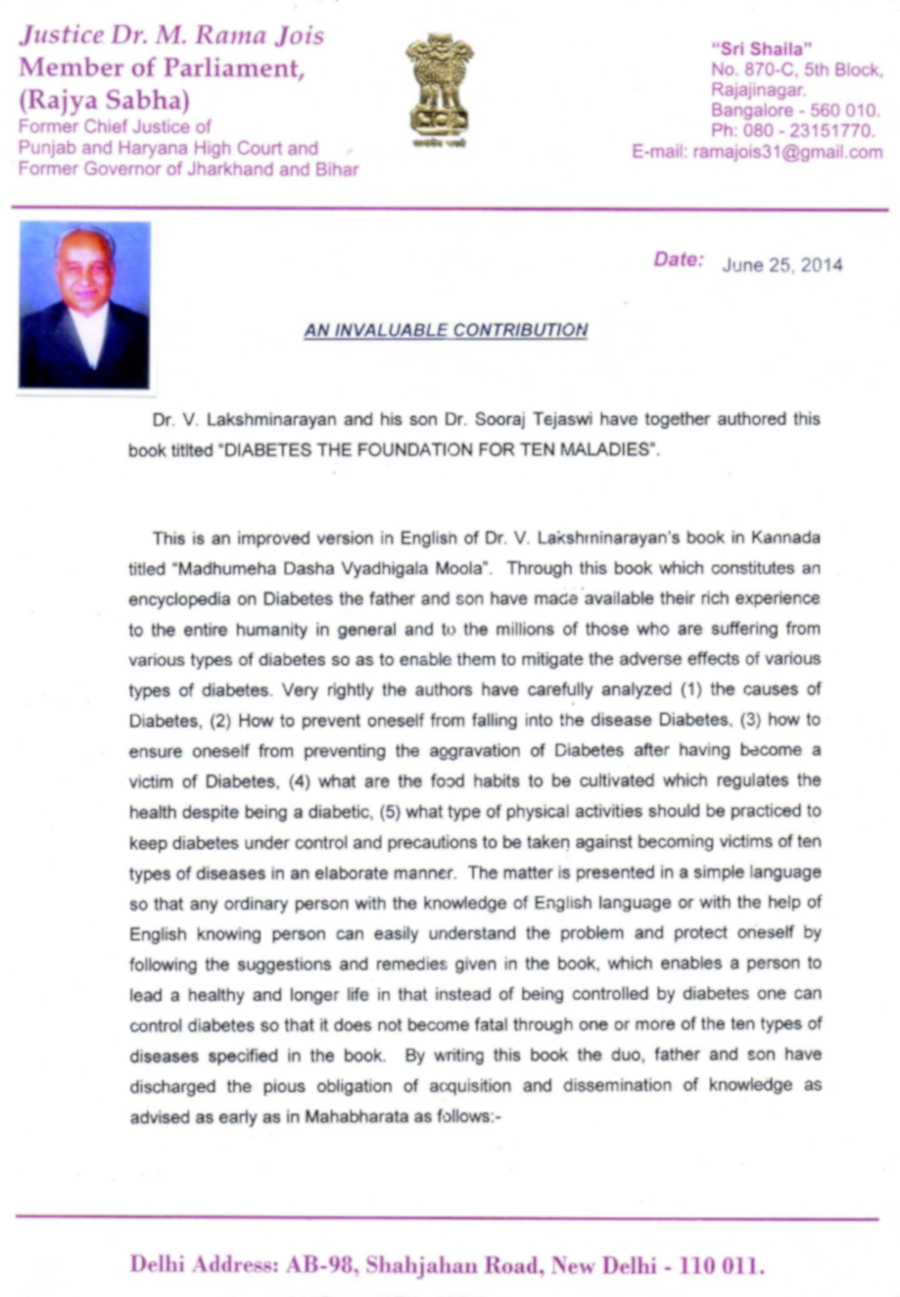
\includegraphics{images/002.jpg}
\caption{\textbf{ಮಾನಸಿಕ ಒತ್ತಡ ಮತ್ತು ಯೋಗ ೧೯ ಸಾಕಷ್ಟು ಆಸಕ್ತಿವಹಿಸಿ ರೋಗಗಳ ಮೂಲವನ್ನು ಕಂಡುಹಿಡಿಯಲಾಗಲಿ ಅಥವಾ ಅದನ್ನು ತಡೆಯಲಿಕ್ಕಾಗಲಿ ಸಾಕಷ್ಟು ಆಸಕ್ತಿ ತೆಗೆದುಕೊಂಡಿಲ್ಲವೆಂಬುದು ಆಶ್ಚರ್ಯಕರ.} }
\end{figure}

ಇಂತಹ ದೊಡ್ಡ ಕಾಯಿಲೆಗಳನ್ನು ತಡೆಗಟ್ಟುವುದಕ್ಕಾಗಿ ತಕ್ಕ ಕಾರ್ಯ ಕ್ರಮಗಳನ್ನು ಶೀಘ್ರ ಕೈಗೊಳ್ಳಲೇಬೇಕಾಗಿದೆ. ಇಲ್ಲವಾದರೆ ಈ ಕಾಯಿಲೆಗಳಿಂದಾಗಿ ಸಾಯುವವರ ಹಾಗೂ ಸಂಪೂರ್ಣ ಅಶಕ್ತರಾಗಿ ಹೋಗುವವರ ಸಂಖ್ಯೆ ಮುಂದೆ ಅದ್ಭುತ ಪ್ರಮಾಣದಲ್ಲಿ ಏರುತ್ತ ಹೋಗುವುದರಲ್ಲಿ ಸಂದೇಹವೇ ಇಲ್ಲ. ಆದ ಕಾರಣ ಈ ಕಾಯಿಲೆಗಳು ಮೂಡಿಬರದಂತೆ ಮಾಡುವುದಕ್ಕಾಗಿ ಎಲ್ಲ ರೀತಿಯ ಕಾರ್ಯಕ್ರಮ ಹಾಕಿಕೊಳ್ಳಬೇಕು; ಮಾತ್ರವಲ್ಲ, ಜನಸಾಮಾನ್ಯರಿಗೆ ಇವು ಹೇಗೆ ಬರುತ್ತವೆ? ಅದನ್ನು ಹೇಗೆ ತಡೆಗಟ್ಟಿ ಬಾಳಿನ ಸಾರ್ಥಕತೆಯನ್ನು ಸಾಧಿಸ ಬಹುದು?—ಮೊದಲಾದ ಅಂಶಗಳನ್ನು ತಿಳಿಯಪಡಿಸುವುದಕ್ಕೂ ತಕ್ಕ ಕಾರ್ಯ ಕ್ರಮ ಅವಶ್ಯ ಹಾಕಿಕೊಳ್ಳಬೇಕಾಗಿದೆ.

\textbf{ಮಾನಸಿಕ ಒತ್ತಡದ ಕಾಯಿಲೆಗಳ ಮೂಲ}

ಮೇಲೆ ಹೇಳಿದ ಅನಾರೋಗ್ಯ ವಿಕಾರಗಳೆಲ್ಲ ಆರಂಭವಾಗುವುದು ಮುಖ್ಯ ವಾಗಿ ಮಾನಸಿಕ ತಳಮಳಗಳ ಮೂಲಕ ಎಂಬುದು ಈಗ ಎಲ್ಲರೂ ಒಪ್ಪಿಕೊಂಡ ವಿಚಾರ. ಅದರ ಪರಿಣಾಮವಾಗಿ ಕ್ರಮೇಣ ದೇಹದ ಒಂದೆರಡು ಇತರ ಪ್ರಮುಖ ಅವಯವಗಳು ಸಹ ತಮ್ಮ ಶಕ್ತಿಯನ್ನು ಕಳೆದುಕೊಳ್ಳುವವು.

ಮೊತ್ತಮೊದಲು ಒತ್ತಡಕ್ಕೆ ಕಾರಣವಾದ ಮಾನಸಿಕ ಉದ್ರೇಕದ ಪ್ರಭಾವ ಇಂದ್ರಿಯಗಳ ಮೂಲಕ ಮಿದುಳಿನ ಬೇರೆಬೇರೆ ನರಕೇಂದ್ರಗಳ ಮೇಲೆ ಬೀಳುತ್ತದೆ. ನಂತರ ಆ ದುಷ್ಪರಿಣಾಮ ಅದರ ಶಕ್ತಿಗನುಗುಣವಾಗಿ ಹರಡುತ್ತ ತಾನಾಗಿಯೇ ಮಿದುಳಿನ ಎಲ್ಲ ನರಕೇಂದ್ರಗಳಿಗೂ ಹಬ್ಬಿಕೊಳ್ಳುತ್ತದೆ. ಆಮೇಲೆ ಮುಖ್ಯವಾಗಿ ಮಿದುಳಿನ ಮೂಲದ ಮತ್ತು ಮೂತ್ರಜನಕಾಂಗದ, ನಿರ್ನಾಳಗ್ರಂಥಿಗಳು \enginline{(Pituitary and Adrenal Glands)} ಕೆಡುತ್ತ ಬಂದು ಕ್ರಮೇಣ ನಿರ್ನಾಳ ಅಂಗಗಳೆಲ್ಲ \enginline{(Endocrine Organs)} ಶಕ್ತಿಹೀನವಾಗುತ್ತವೆ. ಹಾಗೇ ಬರಬರುತ್ತ ಇಡೀ ದೇಹದ ಎಲ್ಲ ಅವಯವಗಳಲ್ಲಿ ಮತ್ತು ಜೀವಕೋಶಗಳಲ್ಲಿ ಜೀವದ್ರವ್ಯಗಳ ಬದಲಾವಣೆಗಳು \enginline{(Metabolic changes)} ಬೆಳೆದುಬರುತ್ತವೆ. ಹೀಗೆ ಉದ್ರೇಕದ ದುಷ್ಟ್ರಭಾವದಿಂದಾಗಿ ದೇಹದ ಎಲ್ಲ ಅಂಗಾಂಗಗಳೂ ಶಕ್ತಿಮೀರಿ ಹೆಚ್ಚಿನ ಕೆಲಸಗೈಯಬೇಕಾಗಿ ಬಂದು ಶಿಥಿಲಗೊಳ್ಳುತ್ತವೆ. ಅದರಲ್ಲಿ ಸಹ ಆನುವಂಶಿಕ ಅಥವಾ ಪರಿಸರದ ಪ್ರಭಾವದಿಂದಾಗಿ ಕೆಲವರಲ್ಲಿ ನಿರ್ದಿಷ್ಟ ಒಂದೆರಡು ಅವಯವಗಳು ವಿಶೇಷವಾಗಿ ನಿಶ್ಯಕ್ತವಾಗುವುದೂ ಉಂಟು. ಇಂತಹ ಸಂದರ್ಭದಲ್ಲಿ ಒಬ್ಬ ವ್ಯಕ್ತಿಯ ನಿರ್ದಿಷ್ಟ ಅವಯವ, ಅತಿಹೆಚ್ಚಿನ ತೊಂದರೆಗೊಳಗಾಗು ವುದು ಹೇಗೆ ಮತ್ತು ಏಕೆ? ಇದು ಒಬ್ಬೊಬ್ಬರಲ್ಲಿ ಒಂದೊಂದು ತರವಾಗುವುದು ಏಕೆ? ಈ ವಿಚಾರದಲ್ಲಿ ಇನ್ನೂ ಆಳವಾದ ಸಂಶೋಧನೆ ನಡೆಯುತ್ತಿದೆ. ಇದಕ್ಕೆ ಆನುವಂಶಿಕವಾದ ನ್ಯೂನತೆ, ಹವಾಮಾನದ ಪ್ರಭಾವ, ಆಹಾರದ ಅಭ್ಯಾಸ, ಸಾಮಾಜಿಕ ಮಾನಸಿಕ ಹಾಗೂ ಪರಿಸರದ ಪ್ರಭಾವ, ಒಬ್ಬೊಬ್ಬರಲ್ಲಿ ಒಂದೊಂದು ತರದ ದುಷ್ಪರಿಣಾಮವನ್ನುಂಟುಮಾಡಲು ಪ್ರಮುಖ ಕಾರಣವಿರಲೂಬಹುದು.

\begin{center}
ಚಿತ್ರ \enginline{3:} ಉತ್ತರಪ್ರದೇಶದ ಪೂರ್ವಭಾಗದ ಕೆಲವು ಆಯ್ದ ಸ್ಥಳಗಳಲ್ಲಿ\\ವ್ಯಾಪಿಸಿರುವ ಹೆಚ್ಚಿದ ರಕ್ತ ಒತ್ತಡ \enginline{\textbf{(Hyper Tension)\\Incidence Of Hypertension in selected areas\\of Eastern U.P.}}
\end{center}


\begin{figure}
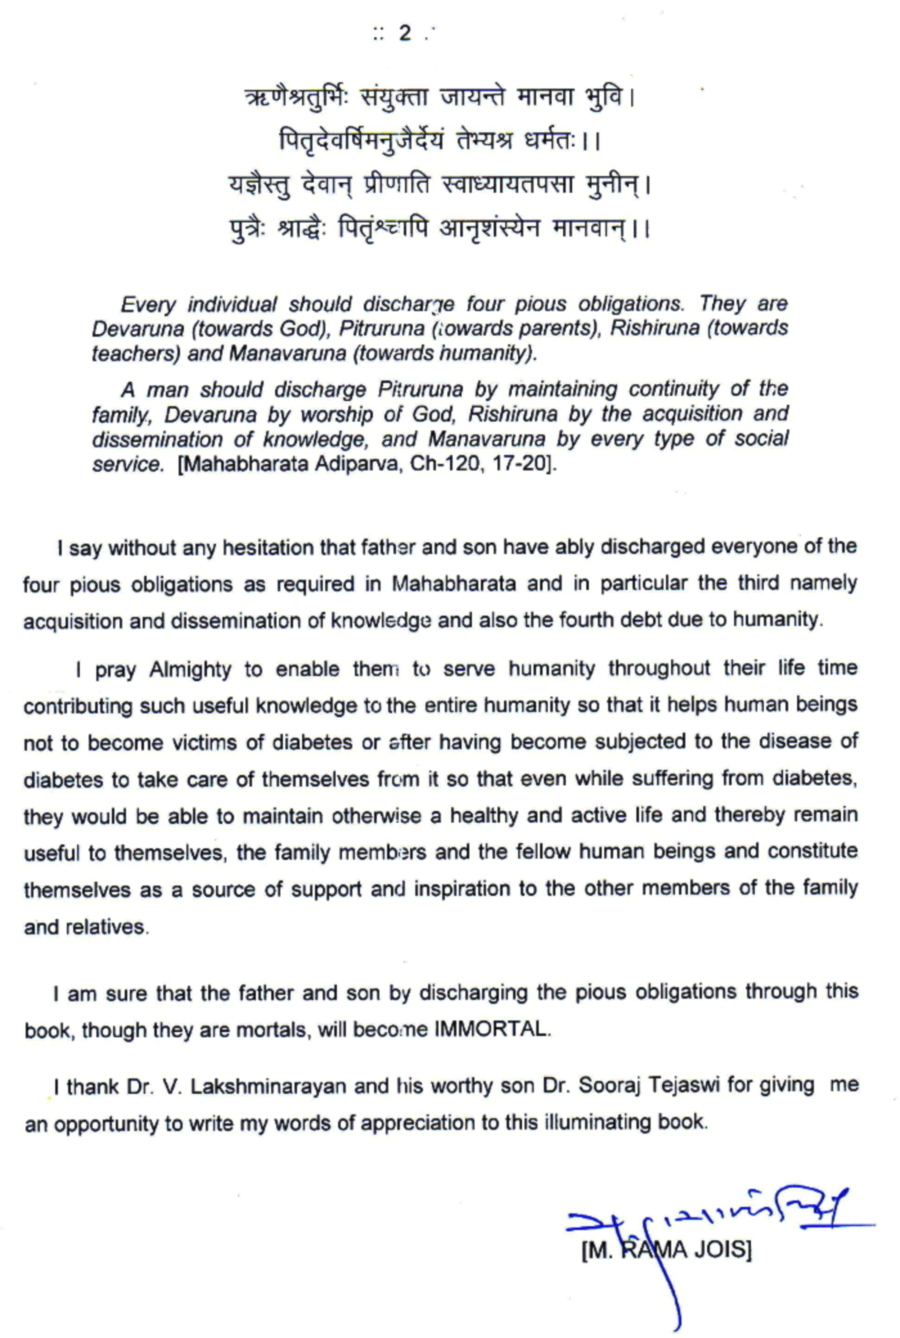
\includegraphics{images/003.jpg}
\caption{ಈ ಹೆಚ್ಚಿದ ರಕ್ತದ ಒತ್ತಡ ಮೂಲ ನಿವಾಸಿ ಜನರಲ್ಲಿ, ಗ್ರಾಮೀಣ ಜನರಲ್ಲಿ ಮತ್ತು ನಗರವಾಸೀ ಜನರಲ್ಲಿ ಬೇರೆಬೇರೆ ಮಟ್ಟದಲ್ಲಿರುವುದನ್ನು ಕಾಣಬಹುದಾಗಿದೆ. ಅದರಲ್ಲೂ ಹೆಂಗಸರಿಗಿಂತ ಗಂಡಸರಲ್ಲೇ ಇದು ಹೆಚ್ಚಿನ ಹಾವಳಿಯನ್ನುಂಟುಮಾಡುತ್ತಿದೆ }
\end{figure}

\begin{center}
ಚಿತ್ರ \enginline{4:} ಉತ್ತರಪ್ರದೇಶದ ಪೂರ್ವಭಾಗದ ಆಯ್ದ ಕೆಲವು ಸ್ಥಳಗಳಲ್ಲಿ ವ್ಯಾಪಿಸಿಕೊಂಡಿರುವ ಉಬ್ಬಸ ಕಾಯಿಲೆ
\end{center}

\begin{center}
\enginline{\textbf{Incidence of Bronchial Asthma in selected areas of Eastern U.P.}}
\end{center}


\begin{figure}
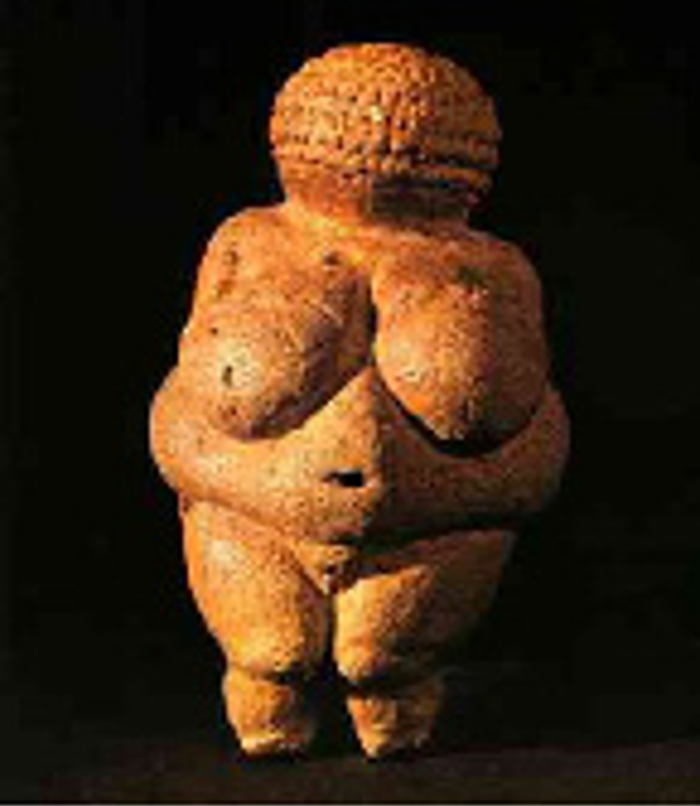
\includegraphics{images/004.jpg}
\caption{ಶ್ವಾಸಕೋಶದ ಉಬ್ಬಸರೋಗ ಒತ್ತಡದಿಂದ ಉಂಟಾಗುವ ಕಾಯಿಲೆಯಾಗಿದೆ. ಇದು ಹಳ್ಳಿಯವರಿಗಿಂತ ಹೆಚ್ಚಾಗಿ ಶಹರಿನಲ್ಲಿರುವವರನ್ನೇ ಕಾಡುತ್ತಿದೆ.}
\end{figure}

ಆದರೆ ಇವೆಲ್ಲ ಮಾನವನ ನಾಗರಿಕಜೀವನದ ಆರಂಭಕಾಲದಿಂದಲೂ ಇದ್ದಿರ ಬಹುದು. ಆದರೂ ಸಹ ಆಧುನಿಕಯುಗದಲ್ಲಿ ಮಿತಿಮೀರಿದ ನಗರೀಕರಣ ದಿಂದಾಗಿ ಮತ್ತು ಮಾನವ–ಮಾನವರೊಳಗಿನ ಸಂಬಂಧ ಸಂಘರ್ಷಗಳಿಂದಾಗಿ ಈ ದುಷ್ಪರಿಣಾಮ ಹೆಚ್ಚುತ್ತ ಬಂದಿರಬಹುದು.

ಹಿಂದೆ ಹೇಳಿದ ಒತ್ತಡ, ಗೊಂದಲಗಳ ಘಟನೆಗಳನ್ನು ಮನಸ್ಸಿನಲ್ಲೇ ಕಲ್ಪಿಸಿ ಕೊಳ್ಳಲೂಬಹುದು. ಸುಖಕರ ಇಲ್ಲವೇ ದುಃಖಕರ ಪ್ರಸಂಗಗಳನ್ನು ಇದ್ದಲ್ಲೇ ಯೋಚಿಸಿಕೊಂಡು ಮೆಲುಕುಹಾಕುತ್ತಲೂ ಇರಬಹುದು. ಇಲ್ಲವೆ, ಮುಂಬರ ಬಹುದಾದ ಭಯಂಕರ ಗಂಡಾಂತರಗಳನ್ನು ಕಲ್ಪಿಸಿಕೊಂಡು ಇದ್ದಲ್ಲೇ ತತ್ತರಿಸಿ ಬೆವತುಕೊಳ್ಳಲೂಬಹುದು. ಮಾನವಜೀವನದಲ್ಲಿ ಮಿತಿಮೀರಿದ ಪ್ರೀತಿ, ದ್ವೇಷ, ಕ್ರೋಧ, ಮಾತ್ಸರ್ಯ, ಮಂತಾದುವುಗಳ ಪರಿಣಾಮವಾಗಿ ಪದೇಪದೇ ಇಂತಹ ಅವಕಾಶಗಳು ಬಂದೇ ಬರುತ್ತವೆ. ಆದಕಾರಣ, ರಾಗ ದ್ವೇಷಗಳ ಮೇಲೆ ಒಂದು ತರದ ಹಿಡಿತ ಇಲ್ಲವಾದರೆ, ಒಂದಲ್ಲ ಒಂದು ತರದ ಒತ್ತಡದಿಂದಾಗುವ ಕಾವು ನೋವುಗಳು ಬರುತ್ತಲೇ ಇರುತ್ತವೆ.

ಇದರಿಂದ ಮತ್ತೊಂದಂಶವೂ ಸ್ಪಷ್ಟವಾಗುತ್ತದೆ. ನಗರವಾಸಿಗಳು ತಮ್ಮ ನಿತ್ಯಜೀವನದಲ್ಲಿ ಗ್ರಾಮವಾಸಿಗಳಿಗಿಂತ ಹೆಚ್ಚಾಗಿ ಸಾಮಾಜಿಕ, ಮಾನಸಿಕ ಉದ್ವೇಗ ಗಳಿಗೊಳಗಾಗಿ ಜೀವನದ ಹೋರಾಟವನ್ನು ನಡೆಸುತ್ತಿದ್ದಾರೆ. ಅದರಿಂದಾಗಿ ಈ ಸಂಕಟಗಳಿಂದ ಹೆಚ್ಚಾಗಿ ನರಳುತ್ತಲೂ ಇದ್ದಾರೆ.

\textbf{ಯೋಗದ ಮೂಲಕ ಒತ್ತಡವನ್ನು ತಡೆಗಟ್ಟುವುದು ಹೇಗೆ?}

ಈಗಿನ ಸಮಾಜದಲ್ಲಿ ಪ್ರತಿಯೊಬ್ಬ ಮಾನವನೂ ಒತ್ತಡದ ಕಾಯಿಲೆಗಳಿಗೆ ಬಲಿ ಯಾಗದಂತೆ ನೋಡಿಕೊಳ್ಳಬೇಕಾಗಿದೆ. ಅದಕ್ಕಾಗಿ ತಕ್ಕ ಪ್ರಯತ್ನ ಕೈಗೊಳ್ಳುವುದೂ ಅತ್ಯಗತ್ಯವಾಗಿದೆ. ಅದಕ್ಕಿರುವ ಒಂದು ದಾರಿಯೆಂದರೆ, ಪ್ರಾಯಶಃ ಈ ನಗರದ ಜಂಜಾಟಗಳಿಂದ ದೂರಹೋಗಿ ಗ್ರಾಮಾಂತರ ಪ್ರದೇಶದ ಪ್ರಶಾಂತ ವಾತಾವರಣ ದಲ್ಲಿ ಹಳೆಯ ಸಾಂಪ್ರದಾಯಿಕ ಜೀವನ ಸಾಗಿಸುವುದಾಗಿದೆ. ಆದರೆ ಇದು ಎಷ್ಟರ ಮಟ್ಟಿಗೆ ಸಾಧ್ಯ? ನಮ್ಮ ಪ್ರಗತಿಯ ಗಡಿಯಾರದ ಮುಳ್ಳನ್ನು ಹಿಂದಕ್ಕೆ ತಿರುಗಿಸುವುದು ಅಷ್ಟು ಸುಲಭವೇ?

ಅದಕ್ಕಿರುವ ಇನ್ನೊಂದು ದಾರಿ, ನಗರದ ಗೊಂದಲಗಳ ಮಧ್ಯದಲ್ಲಿದ್ದು ಮಾನಸಿಕ ಒತ್ತಡ ಮತ್ತು ಯೋಗ ೨೩ ಸಹ ಆ ಗೊಂದಲಗಳ ದುಷ್ಪರಿಣಾಮ ಮಾನವನಿಗೆ ತಾಗದಂತೆ ನೋಡಿಕೊಳ್ಳುವು ದಾಗಿದೆ. ಅದಕ್ಕಾಗಿ, ಆಧುನಿಕ ಜೀವನದಲ್ಲಿ ಬರುವ ಒತ್ತಡದ ಕಾವು ನೋವುಗಳ ವ್ಯಕ್ತಿಯನ್ನು ಕಾಡದಂತೆ ಗೈಯಲು ನಾವು ಉಪಾಯ ಹುಡುಕಬೇಕಾಗಿದೆ.

ಅಪಾಯಕಾರೀ ಸಾಂಕ್ರಾಮಿಕ ರೋಗಗಳ ಹಾವಳಿ ಜನರಿಗೆ ತಾಗದಂತೆ ಉಪಾಯ ನಡೆಸುವುದು ಎಲ್ಲರಿಗೂ ತಿಳಿದಿದೆ. ಮಾನವನಲ್ಲಿ ಸಣ್ಣ ರೂಪದ ಸೋಂಕುರೋಗವನ್ನುಂಟುಮಾಡಿ ಅದರಿಂದ ಪ್ರತಿರೋಧಕಶಕ್ತಿ \enginline{(Immunity)} ಉಂಟಾಗುವಂತೆ ಮಾಡುತ್ತಿರುವುದನ್ನು ನಾವು ತಿಳಿದಿದ್ದೇವೆ. ಅದೇ ತರದಲ್ಲಿ ಮಾನಸಿಕ ಒತ್ತಡದಿಂದ ಬರುವ ಕಾವುನೋವುಗಳನ್ನು ತಡೆಗಟ್ಟುವುದಕ್ಕಾಗಿ ಯೋಗದ ಮೂಲಕ ಸಣ್ಣರೂಪದ ದೈಹಿಕ ಮಾನಸಿಕ ವ್ಯಾಯಾಮಗೈಯಬೇಕು. ಆ ರೀತಿಯ ಪ್ರತಿರೋಧಕಶಕ್ತಿಯನ್ನು ನಾವು ಬೆಳೆಸಿಕೊಂಡು ಹೋಗುವುದು ಪ್ರಯೋಜನಕಾರಿಯಾಗುವುದೆಂದು ಸಂಶೋಧನೆಯಿಂದ ತಿಳಿದುಬಂದಿದೆ.

ಆದರೆ ಈ ಎರಡರಲ್ಲಿ ಒಂದು ವ್ಯತ್ಯಾಸವಿದೆ. ಸಂಕ್ರಾಮಿಕ ರೋಗಗಳ ವಿಷಯದಲ್ಲಿ ಪ್ರತಿರೋಧಕಶಕ್ತಿ ವ್ಯಕ್ತಿಯಲ್ಲಿ ಉಳಿಯಬೇಕಾದರೆ ಆರು ಅಥವಾ ಹನ್ನೆರಡು ತಿಂಗಳಿಗೊಮ್ಮೆ ಪ್ರತಿರೋಧಕ ಚುಚ್ಚುಮದ್ದನ್ನು ತೆಗೆದುಕೊಳ್ಳುತ್ತಿರ ಬೇಕು. ಮಾನಸಿಕ ಒತ್ತಡದ ಕಾಯಿಲೆ ಮಾನವನನ್ನು ಸೋಂಕದಿರಬೇಕಾದರೆ ಪ್ರತಿದಿನ ಯೋಗಾಭ್ಯಾಸದ ಮೂಲಕ ತನ್ನ ದೇಹಮನಸ್ಸುಗಳ ಪ್ರತಿರೋಧಕ ಶಕ್ತಿಯನ್ನು ಬೆಳೆಸಿಕೊಂಡಿರಬೇಕಾಗುತ್ತದೆ. ಮಾನವನಲ್ಲಿ ಮಾನಸಿಕ ಒತ್ತಡದ ಕಾವುನೋವುಗಳು ಬಾರದಂತೆ, ಯೋಗಾಭ್ಯಾಸವು ಹೇಗೆ ಪ್ರತಿರೋಧಕಶಕ್ತಿಯನ್ನು ಬೆಳೆಸುತ್ತದೆ? ಈ ವಿಚಾರವನ್ನೇ ನಾವು ಮುಂದಿನ ಅಧ್ಯಾಯಗಳಲ್ಲಿ ಚರ್ಚಿಸಿ ವಿವರಿಸಲಿದ್ದೇವೆ.

\textbf{ಯೋಗದ ತತ್ವ ಮತ್ತು ಅಭ್ಯಾಸ}

'ಯೋಗ' ಎಂಬ ಪದವನ್ನು ಭಾರತದ ಪ್ರಾಚೀನ ಪುರಾಣಶಾಸ್ತ್ರಗಳಲ್ಲಿ ವಿಭಿನ್ನಾರ್ಥಗಳಲ್ಲಿ ಉಪಯೋಗಿಸಿದ್ದಾರೆ. ಆ ಪದದ ಪ್ರಮುಖ ಅರ್ಥ, 'ಯೋಗ' ಅಂದರೆ ಜೋಡಿಸುವಿಕೆ. ದೇಹ–ಆತ್ಮಗಳ ಭದ್ರವಾದ ಒಂದುಗೂಡುವಿಕೆಯೇ— ಎಂದರ್ಥವಾಗುತ್ತದೆ. ಈ ಗುರಿ ಸಾಧಿಸಲು ಹಲವಾರು ವಿಧಾನಗಳನ್ನು ಹೇಳ ಲಾಗಿದೆ. ಅವುಗಳಲ್ಲಿ, ಪತಂಜಲಿ ಮಹರ್ಷಿಯಿಂದ ಹೇಳಲ್ಪಟ್ಟ ಎಂಟು ವಿಧಾನಗಳುಳ್ಳ ಯೋಗ ಅಥವಾ ಅಷ್ಟಾಂಗ ಯೋಗ ವಿಧಾನ ಅತ್ಯಂತ ಅರ್ಥಯುಕ್ತವಾಗಿದೆ. ಅದು ಬಹಳ ಜನಪ್ರಿಯವಾದ್ದರಿಂದ ಪ್ರಪಂಚದಾದ್ಯಂತ ಜನರು ಅದನ್ನು ಅನುಸರಿ ಸುತ್ತಲೂ ಇದ್ದಾರೆ.

ಇದಲ್ಲದೆ ಶ‍್ರೀಮದ್ಭಗವದ್ಗೀತೆಯಲ್ಲಿ ಭಕ್ತಿಯೋಗ, ಜ್ಞಾನಯೋಗ, ಕರ್ಮ ಯೋಗ ಎಂಬ ಮೂರು ಪಾರಮಾರ್ಥಿಕಯೋಗ ವಿಧಾನಗಳನ್ನೂ ವಿವರಿಸಿ ಹೇಳಿದ್ದಾರೆ. ಅದನ್ನೆಂತು ಜೀವನದಲ್ಲಿ ಅಳವಡಿಸಿಕೊಂಡು ಹೋಗಬೇಕೆಂಬುದನ್ನೂ ತಿಳಿಸಿದ್ದಾರೆ. ಆದರೆ ಇವು ಮುಖ್ಯವಾಗಿ ಪಾರಮಾರ್ಥಿಕಮಾರ್ಗದಲ್ಲಿ ಆದರ್ಶ ಜೀವನವನ್ನು ಸಾಧಿಸಲು ಸೂಚಿತವಾಗಿವೆ. ಇಷ್ಟೇ ಅಲ್ಲದೆ ಜಪಯೋಗ, ಮಂತ್ರ ಯೋಗ, ತಂತ್ರಯೋಗ ಎಂಬವು ಸಹ ಪುರಾಣಗಳಲ್ಲಿ ಹೇಳಲ್ಪಟ್ಟಿವೆ. ಇವು ನಮ್ಮಲ್ಲಿರುವ ನಿಗೂಢಶಕ್ತಿಯನ್ನು ವಿಕಾಸಗೊಳಿಸುವುದಕ್ಕಾಗಿ ಬಳಸಲ್ಪಡಬಹುದಾದವು.

ಎಲ್ಲ ವಿಧದ ಯೋಗವಿಚಾರಗಳನ್ನೂ ನಾವು ಮುಂದಿನ ಪುಟಗಳಲ್ಲಿ ಸಂಕ್ಷೇಪ ವಾಗಿ ಚರ್ಚಿಸಲಿದ್ದೇವೆ. ಆದರೆ ಹೆಚ್ಚಿನ ವಿವರ ಬೇಕೆಂದಿದ್ದರೆ ಮೂಲಗ್ರಂಥಗಳನ್ನೇ ಓದುಗರು ಅಭ್ಯಾಸ ಮಾಡಬೇಕಾಗಬಹುದು.

\textbf{ಕೆಲವು ತಪ್ಪು ತಿಳಿವಳಿಕೆಗಳು}

ಈ ವಿಚಾರದಲ್ಲಿ ಕೆಲವರು ಯೋಗಾಭ್ಯಾಸದಿಂದ ಮಾನವನಲ್ಲಿ ನಿಗೂಢಶಕ್ತಿ ಯೊಂದು ವಿಕಾಸಗೊಳ್ಳುತ್ತದೆ; ಕ್ರಮೇಣ ಅಲೌಕಿಕಸಾಮರ್ಥ್ಯ ಸಹ ಮೂಡಿಬರು ತ್ತದೆ ಎಂದು ಹೇಳುವವರೂ ಇದ್ದಾರೆ. ಆದರೆ ನಾವು ಹಾಗೂ ಇನ್ನು ಕೆಲವಿಜ್ಞಾನಿಗಳು ನಡೆಸಿದ ಅಧ್ಯಯನದ ಪ್ರಕಾರ ಯೋಗವಿಚಾರದಲ್ಲಿ ಅಂತಹ ನಿಗೂಢಶಕ್ತಿ ಯೆಂಬುದು ಇಲ್ಲ. ಆದರೆ ಅಭ್ಯಾಸದಿಂದ ಏನೆಲ್ಲ ಸತ್ಫಲಗಳು ಒದಗಿಬರುತ್ತವೋ, ಅವನ್ನೆಲ್ಲ ವೈಜ್ಞಾನಿಕವಾಗಿ ವಿವರಿಸಬರುತ್ತದೆ. ಯೋಗಾಭ್ಯಾಸದಿಂದ ಹೇಗೆ ಮತ್ತು ಏಕೆ ಉತ್ತಮಮಟ್ಟದ ಪ್ರಯೋಜನ ಪಡೆಯಲಾಗುತ್ತದೆ ಎಂಬುದನ್ನು ಸಕಾರಣ ವಾಗಿ ಸ್ಪಷ್ಟಪಡಿಸಲಾಗುತ್ತದೆ.

ಇದರೊಂದಿಗೆ ನಾವು ಇನ್ನೊಂದಂಶವನ್ನೂ ತಿಳಿದಿರಬೇಕು. ಯೋಗಾಭ್ಯಾಸ ವನ್ನು ಸರಿಯಾಗಿ ತಿಳಿದ ಗುರುವಿನ ಉಪದೇಶ ಪಡೆದು ನಾವು ನಡೆಸಬೇಕು. ದಿಗ್ದರ್ಶನವಿಲ್ಲದ ಸ್ವಯಂಶಿಕ್ಷಣದಿಂದ ತಪ್ಪಾಗಿ ಯೋಗಾಭ್ಯಾಸ ನಡೆಸಿದ್ದಾದರೆ, ಉಪಕಾರಿಯಾಗುವ ಬದಲು ಅದು ಅಪಕಾರಿಯಾಗುವ ಸಂಭವ ಸಹ ಇದೆ. ತಪ್ಪು ವಿಧಾನಗಳಿಂದಾಗಿ ಯೋಗದಿಂದ ಅನಿಷ್ಟಪರಿಣಾಮ ಅನುಭವಿಸಿ ಬೇಸರ ತಳೆದ ವರೂ ಕೆಲವರಿದ್ದಾರೆ.

\textbf{ಅಷ್ಟಾಂಗಯೋಗ}

ಪತಂಜಲಿ ಮಹರ್ಷಿಗಳು ಅಷ್ಟಾಂಗಯೋಗ ಅಥವಾ ಎಂಟು ವಿಧವಾದ ಯೋಗಾ ಭ್ಯಾಸಗಳನ್ನು ಹೇಳಿದ್ದಾರೆ. ಅವುಗಳಲ್ಲಿ ಮೊದಲಿನ ಎರಡು 'ಯಮ' ಅಂದರೆ ಇಂದ್ರಿಯನಿಗ್ರಹ ಮತ್ತು 'ನಿಯಮ' ಅಂದರೆ ವಿವಿಧ ಆಸೆಗಳ ವಿಷಯದಲ್ಲಿ ಸಂಯಮ—ಇವೆರ[ಡು ನೈತಿಕ ಆಧಾರದ ಮೇಲಿವೆ. ಈ ಎರಡು ನೈತಿಕ ಅಭ್ಯಾಸ ಗಳಿಲ್ಲವಾದರೆ ಮುಂದಿನ ಆರು ಯೋಗಾಭ್ಯಾಸಗಳು ಪೂರ್ಣ ಫಲ ಕೊಡಲಾರವು. ಈ ವಿಚಾರದಲ್ಲಿ ಸ್ವಾಮಿ ವಿವೇಕಾನಂದರು ಹೀಗೆ ಹೇಳುತ್ತಾರೆ. 'ಯಮ, ನಿಯಮ ಗಳನ್ನು ಸಾಧಿಸಿದಮೇಲೆಯೇ ಯೋಗಿ ಉಳಿದ ಯೋಗಾಭ್ಯಾಸಗಳನ್ನು ನಡೆಸಬೇಕು; ಆಗಲೇ ಅದರ ಸಂಪೂರ್ಣ ಫಲವನ್ನು ಪಡೆಯಬಲ್ಲವನಾಗುತ್ತಾನೆ. ಇವಿಲ್ಲದೆ ಉಳಿದ ಎಲ್ಲವೂ ವ್ಯರ್ಥ. ಯೋಗಿಯಾದವನು ಕಾಯ, ವಾಕ್, ಮನಸ್ಸುಗಳಿಂದ ಇತರರಿಗೆ ಕೇಡನ್ನು ಬಯಸಬಾರದು. ಮಾನವನ ಮೇಲೆ ಮಾತ್ರ ಕರುಣೆ ತೋರಿದರೆ ಸಾಲದು. ಸಕಲ ಜೀವಜಾತಿಯನ್ನೂ ದಯಾದೃಷ್ಟಿಯಿಂದ ಕಾಣಬೇಕು.' ಅಂತು ಈ ಯಮ ನಿಯಮಗಳು ಮುಂದಿನ ಎಲ್ಲ ಯೋಗಾಭ್ಯಾಸಗಳಿಗೂ ಆಧಾರಸ್ತಂಭ ದಂತಿರುವುದನ್ನು ತಿಳಿದಿರಬೇಕು.

\textbf{ಆಸನ ಅಥವಾ ಅಂಗವಿನ್ಯಾಸ}

ಅಷ್ಟಾಂಗ ಯೋಗಗಳಲ್ಲಿ ಮೂರನೆಯದು 'ಆಸನ' ಅಂದರೆ ಒಂದು ನಿಶ್ಚಿತ ಸ್ಥಿತಿಯ ಅಂಗವಿನ್ಯಾಸ. ಬೇರೆಬೇರೆ ಹಠಯೋಗಗ್ರಂಥಗಳಲ್ಲಿ ಅನೇಕ ವಿಧದ ಅಂಗವಿನ್ಯಾಸ ಕ್ರಮಗಳು ವಿವರಿಸಲ್ಪಟ್ಟಿವೆ. ಇವೆಲ್ಲ ಮುಖ್ಯವಾಗಿ ದೇಹಾರೋಗ್ಯವನ್ನು ಉತ್ತಮಪಡಿಸಲಿರುವ ವ್ಯಾಯಾಮರೂಪದ ಆಸನಗಳಾಗಿವೆ. ಅದರಲ್ಲಿಯೂ ಇವು ನಮ್ಮ ದೇಹದ ಪ್ರಮುಖ ಅಂಗಗಳಾದ—ಮಿದುಳು ಹೃದಯ, ಶ್ವಾಸಕೋಶ, ಯಕೃತ್ತು ಜಠರ ಮತ್ತು ಕರುಳಿನ ಭಾಗಗಳು ಮೂತ್ರಜನಕಾಂಗ—ಮುಂತಾದವುಗಳ ಶಕ್ತಿಯನ್ನು ಸುಧಾರಿಸಲಿರುವ ವ್ಯಾಯಾಮಗಳಾಗಿವೆ. ಇವು ಸ್ನಾಯುಗಳಲ್ಲಿ ರಕ್ತ ಸಂಚಾರವನ್ನು ಹೆಚ್ಚಿಸಿ ಅದರ ಶಕ್ತಿಯನ್ನು ಹೆಚ್ಚಿಸಲಿರುವ ಸಾಂಪ್ರದಾಯಿಕ ದೈಹಿಕ ವ್ಯಾಯಾಮಕ್ಕಿಂತ ಭಿನ್ನವಾಗಿವೆ. ಯೋಗಾಸನಗಳು ಇತರ ಎಲ್ಲ ತರದ ಶಾರೀರಿಕ ವ್ಯಾಯಾಮಗಳಿಂದ ಬೇರೆಯಾದ ರೀತಿಯಲ್ಲಿ ಹೆಚ್ಚಿನ ಪ್ರಭಾವ ಬೀರುತ್ತವೆ. ಅದರಲ್ಲಿಯೂ ವಿಶೇಷವಾಗಿ \enginline{40} ವರ್ಷಕ್ಕೂ ಮೀರಿದ ವಯಸ್ಸಿನವರಿಗೆ ಇದು ಬಹಳ ಉಪಕಾರಿಯಾಗಿದೆ.

ಪ್ರತಿಯೊಬ್ಬನೂ ತಾನು ಮಾಡುವ ಆಸನರೂಪದ ವ್ಯಾಯಾಮವನ್ನು ತನ್ನ ದೇಹಶಕ್ತಿಗನುಗುಣವಾಗಿ ಪ್ರತಿದಿನ ಮಾಡಬೇಕು. ಅಲ್ಲದೆ, ಯಾವುದೇ ಪ್ರಮುಖ ಅಂಗಕ್ಕೆ ಹೆಚ್ಚಿನ ನೋವು ಉಂಟಾಗುವ ತರದಲ್ಲಿ ಪ್ರಯಾಸಪಡಬಾರದು. ಇದರ ಹೆಚ್ಚಿನ ವಿವರಗಳನ್ನು ಮುಂದಿನ ಪುಟಗಳಲ್ಲಿ ವಾಚಕರು ಓದಿಕೊಳ್ಳಬಹುದು. ಆದರೆ ಈಗ ಇಷ್ಟು ಮಾತ್ರ ಹೇಳಬಹುದು. ಈ ಆಸನಗಳ ಸರಿಯಾದ ನಿತ್ಯಾಭ್ಯಾಸ ದಿಂದ ಅದರ ಉತ್ತಮ ಪ್ರಯೋಜನವನ್ನು ಪ್ರತಿಯೊಬ್ಬನೂ ಅರಿತುಕೊಳ್ಳ ಬಹುದು. ಮಾತ್ರವಲ್ಲದೆ, ಅದನ್ನು ವೈಜ್ಞಾನಿಕವಾಗಿ ದೈಹಿಕ ಹಾಗೂ ಜೀವರಾಸಾಯ ನಿಕ ಪ್ರಯೋಗಗಳ ಮೂಲಕ. ಇತರರಿಗೆ ಅರ್ಥವಾಗುವಂತೆ ತೋರಿಸಿಕೊಡಲೂಬಹುದು.

\textbf{ಪ್ರಾಣಾಯಾಮ:} ಪ್ರಾಣ–ಆಯಾಮ ಅಥವಾ ಉಸಿರಾಟದ ವ್ಯಾಯಾಮವು ಯೋಗಾಭ್ಯಾಸದ ಒಂದು ಪ್ರಮುಖ ಅಂಗವಾಗಿದೆ. ನಾವು ಉಸಿರಾಡುವ ಮೂಗಿನ ಎರಡು ರಂಧ್ರಗಳಲ್ಲಿ ಒಂದನ್ನು ಬೆರಳಿಂದ ಮುಚ್ಚಿಕೊಂಡು ಇನ್ನೊಂದರಿಂದ ದೀರ್ಘವಾಗಿ ಶ್ವಾಸವನ್ನು ಒಳಕ್ಕೆ ಸೆಳೆದುಕೊಳ್ಳಬೇಕು. ನಂತರ ಆ ಶ್ವಾಸವನ್ನು ಅಲ್ಲಿಯೇ ಎರಡೂ ರಂಧ್ರಗಳನ್ನು ಮುಚ್ಚಿ ತಡೆಹಿಡಿದುಕೊಳ್ಳಬೇಕು. ಆಮೇಲೆ ಕ್ರಮೇಣ ಇನ್ನೊಂದು ಮೂಗಿನ ರಂಧ್ರದಿಂದ ನಿಧಾನವಾಗಿ ಶ್ವಾಸ ಹೊರಬಿಡ ಬೇಕು.ಆಗ ಬಾಯನ್ನು ಸಂಪೂರ್ಣ ಮುಚ್ಚಿರಬೇಕು. ಇದಾದಮೇಲೆ, ಪುನಃ ಇದೇ ಕ್ರಮವನ್ನು ಬೇರೊಂದು ಮೂಗಿನ ರಂಧ್ರವನ್ನು ಮುಚ್ಚಿ ಉಸಿರಾಟದ ವ್ಯಾಯಾಮ ವನ್ನು ಮುಂದುವರಿಸಬೇಕು. ಒಮ್ಮೆ ಬಲರಂಧ್ರದಿಂದ ಉಸಿರು ತೆಗೆದುಕೊಂಡು ಎಡದಿಂದ ಬಿಡಬೇಕು. ಮತ್ತೊಮ್ಮೆ ಎಡದಿಂದ ಉಸಿರನ್ನು ಮೇಲಕ್ಕೇರಿಸಿ ಬಲ ದಿಂದ ಬಿಡಬೇಕು. ಹೀಗೆ ಸಾಮಾನ್ಯ \enginline{20} ಸಲ ಬೆಳಗ್ಗೆ ಅಥವಾ ಸಂಜೆ ಪ್ರಾಣಾಯಾಮ ಮಾಡುತ್ತಿರಬೇಕು. ಆಗ ಪ್ರತಿಯೊಬ್ಬನೂ ಹೊಸ ಚೈತನ್ಯ ಪಡೆದು ತಾನು ದೇಹ ಮನಸ್ಸುಗಳೆರಡರಲ್ಲೂ ಹಗುರವಾದಂತೆ ಭಾವನೆಗೊಳಗಾಗುತ್ತಾನೆ. ಇದು, ಪ್ರಾಣಾಯಮವನ್ನು ಸರಿಯಾಗಿ ಅಭ್ಯಾಸಮಾಡಿದವರ ಅನುಭವವಾಗಿದೆ.

ಪ್ರಾಣಾಯಾಮದಿಂದ ಪ್ರಾಣಸಂಚಾರ ಸುಧಾರಣೆಯಾಗುತ್ತದೆ. ಹಾಗೆ ಹೆಚ್ಚಿನ ಪ್ರಾಣಶಕ್ತಿ ದೇಹದ ಎಲ್ಲ ನರನಾಡಿಗಳಲ್ಲೂ ತುಂಬಿ ಬರುವ ಕಾರಣ ಆ ರೀತಿಯ ಹೊಸ ಚೈತನ್ಯದ ಅನುಭವ ಒದಗಿಬರುತ್ತದೆ. ಆದಕಾರಣ ಪ್ರತಿದಿನವೂ ನಿಶ್ಚಿತ ಸಮಯದಲ್ಲಿ ಸರಿಯಾಗಿ ಇದನ್ನು ನಡೆಸುತ್ತ ಬಂದರೆ, ಮಾನವ ನವನೂತನ ಚೈತನ್ಯ ಪಡೆದು ನವಜೀವನ ನಡೆಸಲು ಅವಶ್ಯ ಸಮರ್ಥನಾಗುತ್ತಾನೆ.

ಇವನ್ನೆಲ್ಲ ಮಾಡಿ, ನೋಡಿ, ಅನುಭವಿಸಿ ತಿಳಿಯಬೇಕಲ್ಲದೆ ಬರೇ ವಿವರಣೆ ಯಿಂದ ಇದರ ಸಂಪೂರ್ಣ ಅರ್ಥ ಆಗದೆ ಹೋಗಲೂಬಹುದು.

\textbf{ಮಾನಸಿಕ ವ್ಯಾಯಾಮ:} ದೈಹಿಕ ವ್ಯಾಯಾಮರೂಪದ ಯೋಗಾಸನಾ ಭ್ಯಾಸದ ನಂತರ ಅದಕ್ಕೂ ಉಚ್ಚಮಟ್ಟದ ಮಾನಸಿಕ ವ್ಯಾಯಾಮ ರೂಪವಾದ ಯೋಗಾಭ್ಯಾಸವನ್ನು ಕೈಗೊಳ್ಳಬೇಕು. ಅವೇ \enginline{(1)} ಪ್ರತ್ಯಾಹಾರ ಅಂದರೆ ನಮ್ಮ ಬಾಹ್ಯೇಂದ್ರಿಯಗಳನ್ನು ವಿಷಯಸುಖಗಳತ್ತಣಿಂದ ಹಿಂದಕ್ಕೆ ಎಳೆದುಕೊಳ್ಳುವುದು, \enginline{(2)} ಧಾರಣ:ಯಾವುದಾದರೊಂದು ಇಷ್ಟವಸ್ತುವಿನ ಮೇಲೆ ಮನಸ್ಸನ್ನು ಕೇಂದ್ರೀ ಕರಿಸುವುದು, \enginline{(3)} ಧ್ಯಾನ:ನಿರಂತರವಾಗಿ ಆ ಒಂದು ವಸ್ತುವನ್ನೇ ನೆನೆಸಿಕೊಂಡಿರು ವುದು, \enginline{(4)} ಸಮಾಧಿ ಅಂದರೆ, ಕೊನೆಯದಾಗಿ ಆ ಇಷ್ಟವಸ್ತುವಿನಲ್ಲೇ ಲೀನ ಗೊಳ್ಳುವ ದಿವ್ಯಚೈತನ್ಯ ಗಳಿಸುವುದು. ಮಾನಸಿಕ ವ್ಯಾಯಾಮರೂಪವಾದ ಈ ನಾಲ್ಕು ಹಂತಗಳು ಯೋಗಾಭ್ಯಾಸದ ಅಂತಿಮ ಗುರಿಸಾಧನೆಯಲ್ಲಿ ಬಹುಮುಖ್ಯ ವಾದುವು. ಪ್ರತಿದಿನ ಈ ಅಭ್ಯಾಸಗಳನ್ನು ನಿಶ್ಚಿತಸಮಯದಲ್ಲಿ ಶ್ರದ್ಧಾಪೂರ್ವಕವಾಗಿ ನಡೆಸಿಕೊಂಡು ಬಂದರೆ ಮಾತ್ರ ಅದರಿಂದ ಪರಿಪೂರ್ಣಪ್ರಯೋಜನ ಲಭಿಸ ಬಹುದು. ಬದಲಾಗಿ ಅಭಿರುಚಿ ಆಸಕ್ತಿಗಳಿಲ್ಲದೆ ಅರೆಮನಸ್ಸಿನಿಂದ ನಡೆಸಿದ ಯೋಗಾ ಭ್ಯಾಸದಿಂದ ಎಲ್ಲರಿಗೂ ಒಂದೇ ಬಗೆಯ ಉತ್ತಮ ಪ್ರಯೋಜನ ದೊರಕಲಾರದು.

\textbf{ಇತರ ಕಾರ್ಯಕ್ರಮಗಳು:} ಶ್ರದ್ಧಾಪೂರ್ವಕವಾಗಿ ನಿಯತಯೋಗಾಭ್ಯಾಸ ವನ್ನು ನಡೆಸುತ್ತ ಬರುವುದರೊಂದಿಗೆ ಇತರ ಕೆಲವು ಕಾರ್ಯಕ್ರಮಗಳ ಅನು ಸರಣೆಯೂ ಅಗತ್ಯವಾಗಿದೆ. ಮೊತ್ತಮೊದಲಾಗಿ ಮಾನವ ಸೇವಿಸುವ ಆಹಾರ ಪರಿಶುದ್ಧವಾಗಿರಬೇಕು. ಹುಳಿ, ಖಾರ ಮುಂತಾದ ಕಡುಸಾಂಬಾರ ವಿಶೇಷವಾಗಿರದ ಸರಳ ಹಾಗೂ ಮಿತಪ್ರಮಾಣದ ಆಹಾರ ಸೇವಿಸಬೇಕು. ಮಾದಕಪದಾರ್ಥಗಳನ್ನು ಸರ್ವಥಾ ಬಿಡಬೇಕು. ಎಲ್ಲ ವಿಧದ ಬೂಟಾಟಿಕೆಗಳನ್ನು ತೊರೆದು ಸರಳಜೀವನ ನಡೆಸಬೇಕು. ಉದಾತ್ತ ವಿಷಯಗಳ ಮೇಲೆ ಸಮರ್ಥ ಲೇಖಕರು ಬರೆದ ಉತ್ತಮ ಗ್ರಂಥಗಳನ್ನು ಓದುವ ಅಭ್ಯಾಸ ಬೆಳೆಸಿಕೊಳ್ಳಬೇಕು. ಒಂದೇ ಮಾತಿನಲ್ಲಿ ಹೇಳುವು ದಾದರೆ, ಪ್ರಯೋಜನಕ್ಕೆ ಬಾರದ ಆಸಕ್ತಿಗಳನ್ನು ಕಡಿಮೆ ಮಾಡಿಕೊಂಡು, ಈ ಮಾನಸಿಕ ಯೋಗಾಭ್ಯಾಸ ಮುಂದುವರಿಸಿಕೊಂಡು ಹೋಗಬೇಕು.

ಜೀವನಕ್ಕೆ ಸಂಬಂಧಿಸಿದ ಎಲ್ಲ ಹಿತಾಸಕ್ತಿಗಳನ್ನು ಸಂಪೂಣ ತೊರೆದು ಬಿಡ ಬೇಕೆಂದಲ್ಲ. ಕೆಲವೆಲ್ಲ ಉಗ್ರವಾದಿಗಳು ಹೇಳುವಂತೆ, ಕೇವಲ ಯೋಗಾಭ್ಯಾಸ ನಿರತನಾಗಿ ಪರಿಪೂರ್ಣ ಸಂನ್ಯಾಸ ತೆಗೆದುಕೊಳ್ಳಬೇಕೆಂದೂ ಅರ್ಥವಲ್ಲ. ಸಾಮಾನ್ಯ ಮಾನವ ತನ್ನ ಜೀವನಮಾರ್ಗದಲ್ಲಿ ತಕ್ಕ ಆಸಕ್ತಿ ತೋರಲೇಬೇಕು. ತನ್ನ ಉದ್ಯೋಗ ವನ್ನು ಶ್ರದ್ಧೆಯಿಂದ ಎಂದಿನಂತೆ ಸರಿಯಾಗಿ ನಡೆಸಿಕೊಂಡು ಬರಲೇಬೇಕು. ಆದರೆ ತನ್ನ ನಿಯತ ಕೆಲಸಗೈಯುವಾಗ ಉದ್ವೇಗ, ಆವೇಶಗಳಿಗೆ ಒಳಗಾಗಬಾರದು. ಮಾನಸಿಕ ಸಮತೋಲನವನ್ನು ದಿನವಿಡೀ ಕಾಪಾಡಿಕೊಂಡು ಬರಬೇಕು. ಯೋಗತತ್ವ ವನ್ನು ತನ್ನ ಕರ್ಮಮಾರ್ಗದಲ್ಲಿ ಅಳವಡಿಸಿಕೊಂಡು ಬರಲು ತಿಳಿದಿರಬೇಕು. ಇದೀಗ ಯೋಗಭ್ಯಾಸದಿಂದ ಒದಗಿಬರುವ ನಿಜವಾದ ಪ್ರಯೋಜನವಾಗಿದೆ. ಇದರ ಸರಿಯಾದ ಅಭ್ಯಾಸ, ಆಚರಣೆ ಗೈಯುವುದರಿಂದ ಮಾನವ ತನ್ನ ಜೀವನವನ್ನು ಸಫಲಗೊಳಿಸಲು ಅವಶ್ಯ ಸಮರ್ಥನಾಗುತ್ತಾನೆ.

ಜೀವನದಲ್ಲಿ ಒದಗುವ ಒತ್ತಡದ ಕಾವುನೋವುಗಳಿಂದಾಗಿ ಮನುಷ್ಯನಿಗೆ ಎಳೆತನದಲ್ಲೇ ಮುದಿತನದ ಲಕ್ಷಣಗಳು ಮೂಡಿಬರುತ್ತವೆ. ಕ್ರಮಪ್ರಕಾರವಾದ ಯೋಗಾಭ್ಯಾಸದಿಂದ ವೃದ್ಧಾಪ್ಯದ ಆಗಮನ ದೂರವಾಗುವುದು ಮಾತ್ರವೇ ಅಲ್ಲ; ಆಯುಷ್ಯದ ವೃದ್ಧಿಯೂ ಹೆಚ್ಚಿನೆಡೆ ಬಂದೇ ಬರುತ್ತದೆ. ಈ ಸಂದರ್ಭದಲ್ಲಿ \enginline{110} ವರ್ಷ ಬದುಕಿರುವ ಮಿ~। ಆರ್ನಾಲ್ಡ್ ಅವರ ಅನುಭವ ನಿಜವಾಗಿಯೂ ಓದುಗರ ಮೇಲೆ ಹೊಸ ಬೆಳಕು ಬೀರುವುದರಲ್ಲಿ ಸಂದೇಹವಿಲ್ಲ.

ಮಿ~। ಆರ್ನಾಲ್ಡ್ ಅವರು \enginline{110} ವರ್ಷದ ವಯಸ್ಸಿನಲ್ಲಿಯೂ ತನ್ನ ಎಲ್ಲ ಅವಯವಗಳಮೇಲೂ, ಚುರುಕಾದ ಬುದ್ಧಿ ಮನಸ್ಸುಗಳ ಮೇಲೂ ಸಂಪೂರ್ಣ ಹಿಡಿತ ಹೊಂದಿದವರಾಗಿದ್ದರು. \enginline{1952} ರಲ್ಲಿ ಕಾಶಿಯಲ್ಲಿ ಆಕಸ್ಮಿಕವಾಗಿ ದೊರಕಿದ ಯೋಗಗುರು ಚಕ್ರಾನಂದರ ಉಪದೇಶದಿಂದ ಯೋಗಾಭ್ಯಾಸವನ್ನಾರಂಭಿಸಿ ನಿತ್ಯ ನಡೆಸಿಕೊಂಡು ಬರುತ್ತಿದ್ದು ಚುರುಕುಜೀವನ ನಡೆಸುತ್ತಿದ್ದರು. ಅವರ ಅನುಭವ ಅವಶ್ಯ ತಿಳಿಯಬೇಕಾದ್ದಾಗಿದೆ. ಅವರ ಪತ್ರದ ಪೂರ್ಣಪಾಠವನ್ನು ಅನುಬಂಧ \enginline{(Appendix)} ದಲ್ಲಿ ಕೊಡಲಾಗಿದೆ.

\textbf{ಯೋಗ ತತ್ವ:} ವಿಜ್ಞಾನದಲ್ಲಿ ಯಾವುದೇ ಒಂದು ವಿಚಾರದ ಸತ್ಯಾಸತ್ಯತೆ ಯನ್ನು ಸರಿಯಾಗಿ ಪರಿಶೀಲಿಸಿ ವಿಜ್ಞಾನಿ ಅಳೆದು ನೋಡಬಲ್ಲವನಾಗುತ್ತಾನೆ. ಹಿಂದಿನ ಕಾಲದಲ್ಲಿ ಕೇವಲ ವಸ್ತುನಿಷ್ಠವಾದ ಪರಿಶೀಲನೆ ನಡೆಸಿ ವಿವಿಧ ವೈಜ್ಞಾನಿಕ ಸತ್ಯವನ್ನು ಅಳೆದು ನೋಡುವುದಿತ್ತು. ಆದರೆ ಇತ್ತೀಚಿನ ವರ್ಷಗಳಲ್ಲಿ ವ್ಯಕ್ತಿನಿಷ್ಠ ವಾದ ಪರೀಕ್ಷೆಗಳಿಂದಲೂ ಮನೋವೈಜ್ಞಾನಿಕ ಹಾಗೂ ದೈಹಿಕ ವಿಚಾರಗಳನ್ನು ಪರಿಶೀಲಿಸಿ ಅಳೆದು ನೋಡುವುದುಂಟು.

ಯೋಗಾಭ್ಯಾಸದ ಪರಿಣಾಮವನ್ನು ವ್ಯಕ್ತಿನಿಷ್ಠ ಹಾಗೂ ವಸ್ತುನಿಷ್ಠ ವಿಧಾನ ಗಳಿಂದ ಅಳೆದುನೋಡಲು ಸಾಧ್ಯವಾಗುತ್ತಿದೆ. ಆರಂಭದೆಸೆಯಲ್ಲಿ ವ್ಯಕ್ತಿಗತ ಅನು ಭವಗಳೇ ಸಂಶೋಧನೆಗೆ ಮೂಲವಸ್ತುವಾಗುತ್ತದೆ. ಕ್ರಮೇಣ ಯೋಗಾಭ್ಯಾಸದಿಂದ ಉಂಟಾಗುವ ಬದಲಾವಣೆಗಳನ್ನು ವಸ್ತುನಿಷ್ಠ ಪರೀಕ್ಷೆಗಳಿಂದಲೂ ಅಳೆದು ನೋಡ ಲಾಗುತ್ತಿದೆ.

ಕೆಲವೆಲ್ಲ ವಿಶಿಷ್ಟ ಯೋಗಾಭ್ಯಾಸಗಳನ್ನು ಕ್ರಮಬದ್ಧವಾದ ರೀತಿಯಲ್ಲಿ ನಡೆಸಿ ಕೊಂಡು ಬರುತ್ತಿರುವ ನಮ್ಮ ಸ್ವಯಂಸೇವಕರಲ್ಲಿ ನಿಚ್ಚಿತಕಾಲಾನಂತರ ಮೂಡಿ ಬಂದ ಸುಧಾರಣೆಗಳನ್ನು ಪರಿಶೀಲಿಸಲಾಯಿತು. ಆಗ, ಕೆಲವೆಲ್ಲ ದೈಹಿಕಮಾನಸಿಕ ಬದಲಾವಣೆಗಳನ್ನು ಆಧುನಿಕ ಸಂಶೋಧಕದೃಷ್ಟಿಯಿಂದ ಅಳೆದು ನೋಡಿ ತೋರಿಸಲು ಸಾಧ್ಯವಾಯಿತು. ಇದು ನಿಜವಾಗಿಯೂ ಸಂತೃಪ್ತಿಯನ್ನು ಉಂಟು ಮಾಡಿದ ವಿಷಯವಾಗಿದೆ.

ಈ ಸುಧಾರಣೆಗಳು ನಿಗದಿತ ಯೋಗಾಭ್ಯಾಸವನ್ನು ಸರಿಯಾಗಿ ಮಾಡಿಕೊಂಡು ಬಂದ ಎಲ್ಲ ಸ್ವಯಂಸೇವಕರಲ್ಲಿಯೂ ಸಮಾನರೀತಿಯಲ್ಲಿ ತೋರಿಬಂದವು. ಅಷ್ಟೇ ಅಲ್ಲದೆ ಸ್ವಯಂಸೇವಕರ ಶರೀರವೈಜ್ಞಾನಿಕ \enginline{(physiological)} ಮತ್ತು ಜೀವ ರಾಸಾಯನಿಕ ಪರೀಕ್ಷೆಗಳನ್ನು ನಡೆಸಿ, ದೇಹದ ಪ್ರತಿಭಾಗವನ್ನೂ ಪರಿಶೀಲಿಸಿ ನೋಡಿದರೂ ಒಂದೇ ಬಗೆಯ ಸುಧಾರಣೆಗಳು ತೋರಿಬಂದುವು. \enginline{Neuro} \enginline{}\enginline{humoral studies, Electro Encephalographic studies and differednt Harmonal and Metabolic studies} ಗಳನ್ನು ಸಹ ಪರಿಶೀಲಿಸಿ ನೋಡಿದಾಗ ನಿರಂತರವಾಗಿ ಒಂದೇತರದ ಫಲಿತಾಂಶಗಳು ತೋರಿಬಂದುವು. ಅವು ಯಾವುದೇ ವ್ಯಕ್ತಿಯಲ್ಲಿ ಬೇಕಾದಾಗ ಅಂತಹ ಅಭ್ಯಾಸದಿಂದ ಮೂಡಿಸಿ ತರಲು ಸಾಧ್ಯವಾಗುವ ತರದಲ್ಲಿಯೂ ಇದ್ದುವು. ಇದರ ಹೆಚ್ಚಿನ ವಿವರಗಳನ್ನು ಮುಂದಿನ ಅಧ್ಯಾಯಗಳಲ್ಲಿ ತಿಳಿಸಲಿದ್ದೇವೆ.

ಈ ವೈಜ್ಞಾನಿಕ ಸತ್ಯವನ್ನು ಒಪ್ಪಿಕೊಳ್ಳುವ ವಿಚಾರದಲ್ಲಿ ಜಗತ್ತಿನಾದ್ಯಂತ ಯಾವ ಸಂದೇಹವೂ ಉಳಿಯದಂತಾಗಿದೆ.

ವಿಜ್ಞಾನ ಮತ್ತು ಊಹೆಗಳ ಮಧ್ಯವರ್ತಿಗಳೆಂದು ಹೇಳಬಹುದಾದ ಕೆಲವಂಶ ಗಳೂ ಇವೆ. ಎಲ್ಲ ವಿಜ್ಞಾನಿಗಳಿಗೂ ಇಂತಹ ವ್ಯಕ್ತಿನಿಷ್ಠ ಅನುಭವಗಳನ್ನು ವೈಜ್ಞಾನಿಕ ಸತ್ಯವೆಂದು ನಂಬದಿರಬಹುದು. ಅಂತಹ ಅನುಭವಗಳು ಸಮರ್ಥ ಗುರುವಿನ ಅನುಗ್ರಹದಿಂದ ಅಭ್ಯಾಸಗೈದ ಕೆಲವರಿಗೆ ಮಾತ್ರ ಗೋಚರವಾಗಬಹುದು. ಅಂಥ ವರಿಗೆ ಸತ್ಯವೆಂದಾಗಲೂಬಹುದು.

ಆ ರೀತಿಯ ಗುರುವಿನ ಗುಲಾಮನಾಗುವ ಅವಕಾಶ ಜಗತ್ತಿನಲ್ಲಿ ಕೆಲವರಿಗೆ ಮಾತ್ರ ದೊರಕಬಹುದು. ಆದ್ದರಿಂದ ಆತ್ಮಾನುಭವಗಳು ಇತರರಮಟ್ಟಿಗೆ ಕೇವಲ ಊಹೆಯೆಂದೇ ಭಾವಿಸಲ್ಪಡಬಹುದು. ಈ ಸಂದರ್ಭದಲ್ಲಿ ಸ್ವಾಮಿ ವಿವೇಕಾನಂದರ ಈ ಕೆಳಗಿನ ಮಾತುಗಳನ್ನು ನಾವು ಸ್ಮರಿಸಿಕೊಳ್ಳಬಹುದಾಗಿದೆ.

"ರಾಜಯೋಗವೆಂಬ ವೈಜ್ಞಾನಿಕ ಸಾಧನವು ನಮ್ಮ ಅನಂತಶಕ್ತಿಯನ್ನು ಕಂಡು ಕೊಳ್ಳಲು ಸಹಾಯಕವಾಗುತ್ತದೆ. ಈ ಸಾಧನ ಮೂಲತಃ ಮನಸ್ಸೇ ಆಗಿರುತ್ತದೆ. ಅದನ್ನು ಕೇಂದ್ರೀಕರಿಸಿ ಅಂತರಾತ್ಮನನ್ನು ತಿಳಿಯಲು ಪ್ರಯತ್ನಿಸಿದಾಗ, ಆತ್ಮ ಮನಸ್ಸುಗಳೆರಡರ ಮೇಲೂ ಬೆಳಕು ಬಿದ್ದಂತಾಗುತ್ತದೆ. ಆಂತರಿಕ ಮನಸ್ಸಿನ ಶಕ್ತಿ, ಬೆಳಕಿನಂತೆ. ಅದನ್ನು ಹಾಗೆಯೇ ಬಿಟ್ಟರೆ ಬೆಳಕು ಸುತ್ತ ಹಬ್ಬಿಕೊಂಡಿರುತ್ತದೆ. ಅದನ್ನು ಒಂದು ವಿಷಯದತ್ತ ಕೇಂದ್ರೀಕರಿಸಿಕೊಂಡಾಗ ಆ ವಸ್ತುವನ್ನು ಆಳವಾಗಿ ಮತ್ತು ಸಮಗ್ರವಾಗಿ ತಿಳಿದುಕೊಳ್ಳಲು ಸಹಾಯವಾಗುತ್ತದೆ. ಅದೇ ತರದಲ್ಲಿ ನಮ್ಮ ಮನಸ್ಸಿನ ಶಕ್ತಿಯನ್ನು ಎಳೆತನದಿಂದಲೂ ಬಾಹ್ಯವಸ್ತುಗಳನ್ನು ಅರಿತುಕೊಳ್ಳುವುದಕ್ಕೆ ಮಾತ್ರ ಬಳಸಲು ನಾವು ತಿಳಿದಿರುತ್ತೇವೆ. ಬದಲಾಗಿ ಅದನ್ನು ಅಂತದರ್ಶನಕ್ಕೆ ಬಳಸಿ, ಕೇಂದ್ರೀಕರಿಸಿದಾಗ ಆ ಮನಸ್ಸಿನ ಅಪಾರಶಕ್ತಿಯನ್ನು ಅರಿತುಕೊಳ್ಳ ಬಹುದಾಗಿದೆ."

ಈ ದಾರಿಯಲ್ಲಿ ಮುಂದುವರಿದು ಮನಃಶಕ್ತಿಯ ವೈಜ್ಞಾನಿಕ ಅಧ್ಯಯನ ನಡೆಸಲು ನಮಗೆ ಸಾಧ್ಯವಾಗಿದೆ. ವಿವೇಕಾನಂದರು ಇನ್ನೂ ಕೆಲವಿಚಾರ ಹೇಳಿದ್ದಾರೆ. "ಪ್ರಪಂಚದ ಅಪಾರ ವೈಭವದ ಗುಟ್ಟನ್ನು ನಾವು ಅರಿತುಕೊಳ್ಳಬೇಕಾದರೆ ಬಲವಾದ ಕೇಂದ್ರೀಕೃತ ಶಕ್ತಿಯಿಂದ ಬಲವಾಗಿ ಬಡಿದು ನೋಡಬೇಕಾಗಿದೆ. ಆ ಶಕ್ತಿ ಬರುವುದು ಮನಸ್ಸನ್ನು ಕೇಂದ್ರೀಕರಿಸಿ ಬಲಪಡಿಸುವುದರಿಂದ ಮಾತ್ರ ಸಾಧ್ಯ. ಮಾನವಮನಸ್ಸಿನ ಆ ಶಕ್ತಿಗೆ ಮಿತಿಯೇ ಇಲ್ಲ. ನಾವೆಷ್ಟರಮಟ್ಟಿಗೆ ಮನಸ್ಸನ್ನು ಕೇಂದ್ರೀಕರಿಸಿ ಬಲ ಪಡಿಸಿಕೊಳ್ಳುತ್ತೇವೋ ಅಷ್ಟೇ ಹೆಚ್ಚಿನ ಶಕ್ತಿಯನ್ನು ನಾವು ಸಾಧಿಸಿಕೊಳ್ಳಬಹುದು. ನಮ್ಮ ಕೇಂದ್ರೀಕರಣಶಕ್ತಿಗನುಗುಣವಾಗಿ ಮನಶ್ಯಕ್ತಿಯು ಬೆಳೆದುಬರುತ್ತದೆ. ಇದು ಪರಮ ರಹಸ್ಯ ವಿಚಾರವಾಗಿದೆ."

\textbf{ಮನಸ್ಸಿನ ಕೇಂದ್ರೀಕರಣ ಅಥವಾ ಏಕಾಗ್ರತೆ:} ಮೇಲೆ ಹೇಳಿದ ವಿಷಯ ಗಳಿಂದ ಒಂದಂಶ ಸ್ಪಷ್ಟವಾಗುತ್ತದೆ. ನಾವು ಮನಸ್ಸನ್ನು ಏಕಾಗ್ರಭಾವದಿಂದ ಒಂದು ವಿಷಯದಲ್ಲಿ ಕೇಂದ್ರೀಕರಿಸಿಕೊಂಡಿರಲು ಸರಿಯಾದ ಅಭ್ಯಾಸಗೈದು ಕಲಿತುಕೊಂಡಿರ ಬೇಕು. ಆಗ ತೋರಿಬರುವ ಮಾನಸಿಕ ಹಾಗೂ ದೈಹಿಕ ಬದಲಾವಣೆಗಳನ್ನು ಅನುಭವದಿಂದ ಅರಿತುಕೊಳ್ಳಲು ಸಾಧ್ಯವಾಗಬಹುದು. ಅಷ್ಟೇ ಅಲ್ಲದೆ ಕ್ರಮೇಣ ಈ ತರದ ಆಂತರಿಕ ಬದಲಾವಣೆಗಳನ್ನು ಆಧುನಿಕ ವೈಜ್ಞಾನಿಕ ಉಪಕರಣಗಳಿಂದ ಅಳೆದು ತಿಳಿದುಕೊಳ್ಳಲೂ ಸಾಧ್ಯವಾಗಬಹುದು.

ಮನಸ್ಸಿನ ಏಕಾಗ್ರತೆಯನ್ನು ಹೇಗೆ ಮತ್ತು ಎಷ್ಟರಮಟ್ಟಿಗೆ ಸಾಧಿಸಬಹುದೆಂಬು ದನ್ನು ಈಗಿನ ವೈಜ್ಞಾನಿಕ ಉಪಕರಣಗಳಿಂದ ಸರಿಯಾಗಿ ಅಳೆದು ನೋಡುವ ಸಾಧ್ಯತೆ ಸಾಕಷ್ಟಿಲ್ಲ. ಏಕಾಗ್ರತೆಯ ಗಾಢತೆ ವ್ಯಕ್ತಿಯಿಂದ ವ್ಯಕ್ತಿಗೆ ಅವರವರ ದೇಹ ಮನಶ್ಯಕ್ತಿ ಗಳಿಗನುಗುಣವಾಗಿ ಭಿನ್ನಭಿನ್ನವಾಗಿರಲೂಬಹುದು. ಆದಕಾರಣ ಈ ಕೇಂದ್ರೀಕೃತ ಮನಶ್ಯಕ್ತಿಯ ಪ್ರಭಾವವನ್ನು ಸರಿಯಾಗಿ ಅಳೆದು ನೋಡುವ ಉಪಕರಣಗಳ ಆವಿಷ್ಕಾರವಾಗುವತನಕ ನಾವು ಊಹೆ ಮತ್ತು ವೈಜ್ಞಾನಿಕ ಸತ್ಯಗಳ ಸಮೀಪವರ್ತಿ ವಿಚಾರವೆಂದು ಹೇಳಬಹುದಾಗಿದೆ.

\textbf{ಯೋಗತತ್ವಗಳ ಮೂಲ:} ಯೋಗಾಭ್ಯಾಸದಲ್ಲಿ ಅನುಸರಿಸಲಾಗುವ ತತ್ವ ಶಾಸ್ತ್ರದ ಮೂಲ ಹೆಚ್ಚಿನಂಶ ಭಗವದ್ಗೀತೆಯಲ್ಲಿದೆ. ಇದರಲ್ಲಿ ಜೀವನದ ಸಮಸ್ಯೆ ಗಳ ಪರಿಹಾರ ಮಾರ್ಗ ತಿಳಿಯಲು, ವಿವಿಧ ಯೋಗಾಭ್ಯಾಸದ ಮೂಲಕ ಸಾಧ್ಯ ವೆಂದು ವಿವರಿಸಲಾಗಿದೆ. ಪ್ರಪಂಚದಲ್ಲಿ ಸಾತ್ವಿಕ, ರಾಜಸ, ತಾಮಸ ಸ್ವಭಾವಗಳಿಂದ ಕೂಡಿದ ಮೂರು ತರದ ಜನರಿದ್ದಾರೆ. ಸಾತ್ವಿಕ ಅಂದರೆ ಸಾಧುಸ್ವಭಾವದ, ರಾಜಸ ಅಂದರೆ ಕ್ರೂರಸ್ವಭಾವದ, ತಾಮಸ ಅಂದರೆ ಮಾಯಾ (ಅಜ್ಞಾನ) ಸ್ವಭಾವದ ಮಾನವರಿದ್ದಾರೆ. ಈ ತರದ ವ್ಯಕ್ತಿಗುಣಕ್ಕನುಗುಣವಾದ ಯೋಗಾಭ್ಯಾಸ ವನ್ನಾರಂಭಿಸಿ ತಮ್ಮತಮ್ಮ ಯೋಗ್ಯತೆಯನ್ನು ಉತ್ತಮಪಡಿಸಿಕೊಳ್ಳಬೇಕೆಂದು ಗೀತೆಯಲ್ಲಿ ವಿವರಿಸಿದ್ದಾರೆ. ಕರ್ಮಯೋಗ, ಭಕ್ತಿಯೋಗ, ಜ್ಞಾನಯೋಗ ಎಂಬ ಮೂರು ತರದ ಯೋಗಮಾರ್ಗಗಳನ್ನನುಸರಿಸಿ ಮಾನವ ಉತ್ತಮತೆಯನ್ನು ಸಾಧಿಸಬಹುದಾಗಿದೆ ಎಂದೂ ಹೇಳಿದ್ದಾರೆ.

ಸಂಕ್ಷೇಪವಾಗಿ ತ್ರಿವಿಧ ಯೋಗಗಳ ತತ್ವವನ್ನು ಹೇಳುವುದಾದರೆ,

\enginline{1} \textbf{ಕರ್ಮಯೋಗ:} ನಿರಂತರವಾದ ಹಾಗೂ ಫಲಾಪೇಕ್ಷೆಯಿಲ್ಲದ, ಹೃತ್ಪೂರ್ವಕ ಕೆಲಸದ ಮೂಲಕ ದೇವರ ಪ್ರೀತಿ ಅಥವಾ ದಯೆಯನ್ನು ಗಳಿಸುವುದು.

\enginline{2} \textbf{ಭಕ್ತಿಯೋಗ:} ಪರಮಾತ್ಮನ ಮೇಲಿನ ನಿರಂತರ ಪ್ರೀತಿಭಕ್ತಿಗಳಿಂದ ದೇವರನ್ನು ಒಲಿಸಿಕೊಳ್ಳುವುದು.

\enginline{3} \textbf{ಜ್ಞಾನಯೋಗ:} ಆಧ್ಯಾತ್ಮಿಕ ತತ್ವಜ್ಞಾನವನ್ನು ಬೆಳೆಸಿಕೊಂಡು ಪರಮಾತ್ಮ ನನ್ನು ಅರಿತುಕೊಳ್ಳುವುದು.

ಈ ಮೂರು ಯೋಗ ಮಾರ್ಗಗಳಿಂದ ಅವರವರ ಶಕ್ತಿಗನುಗುಣವಾಗಿ ಸಾಧಿಸಿ, ದೇವರನ್ನು ಒಲಿಸಿಕೊಳ್ಳುವ ವಿಚಾರವನ್ನು ಗೀತೆಯಲ್ಲಿ ಹೇಳಿದ್ದಾರೆ. ಪ್ರಪಂಚದ ವಿವಿಧ ಮಟ್ಟದ ವಿವಿಧ ರೀತಿಯ ಜನರು ತಮ್ಮತಮ್ಮ ಶಕ್ತಿ ಯೋಗ್ಯತೆ ಗಳಿಗನುಗುಣವಾದ ಮೂರು ಅಥವಾ ಅವುಗಳಲ್ಲಿ ಒಂದೆರಡಾದರೂ ಯೋಗ ಮಾರ್ಗವನ್ನನುಸರಿಸಿ ಉದಾತ್ತ ಗುಣಗಳನ್ನು ಸಾಧಿಸಬೇಕೆಂದೂ ಹೇಳಿದ್ದಾರೆ.

\textbf{ಕುಂಡಲಿನೀ ಯೋಗ:} ತಂತ್ರಶಾಸ್ತ್ರದ ಪ್ರಕಾರ ನಮ್ಮ ದೇಹದಲ್ಲಿ ಆರು ಚಕ್ರ ಅಥವಾ ನರಕೇಂದ್ರಗಳಿವೆ. ಅವುಗಳಲ್ಲಿ ಅತ್ಯಂತ ಕೆಳಗಿನದು ಮೂಲಾಧಾರ ಚಕ್ರ \enginline{(Perineum)}. ತುತ್ತತುದಿಯದು ಹಣೆಯ ಮೇಲಿನ ಸಹಸ್ರಾರಚಕ್ರ. ಆರು ಕೇಂದ್ರ ಗಳೊಳಗೆ ಸೂಕ್ಷ್ಮನಾಡಿಗಳ ಮೂಲಕ ಒಂದಕ್ಕೆ ಇನ್ನೊಂದರ ಸಂಬಂಧವಿದೆ. ಆ ನಾಡಿಗಳಲ್ಲಿ ಇಡಾ, ಪಿಂಗಳಾ, ಸುಷುಮ್ನಾ ನಾಡಿಗಳು ಮುಖ್ಯವಾದವುಗಳು. ಆಧುನಿಕ ದೇಹಶಾಸ್ತ್ರದ ಪ್ರಕಾರ ಈ ಚಕ್ರಗಳನ್ನು \enginline{Autonomic Ganglia} ಎಂದು ಕರೆಯಲ್ಪಡುವ ವಿಭಿನ್ನ ಸ್ವತಂತ್ರ ನರಕೇಂದ್ರಗಳಿಗೆ ಸಮಾನವಾದವುಗಳೆಂದು ಹೇಳಬಹುದು. ಅನುವೇದನಾ ಮತ್ತು ಸಹಾನುವೇದನಾ ನರವ್ಯೂಹ ಕೇಂದ್ರವಾದ (Sympathetic and Para–Sympathetic Nerve Centre) ಸಹಸ್ರಾರು ಚಕ್ರವನ್ನು ಮಿದುಳಿನ ಕೇಂದ್ರಸ್ಥಾನವೆಂದು \enginline{(Hypothalmic Region)} ಹೇಳ ಬಹುದು. ಇಡಾ ಪಿಂಗಳಾ ನಾಡಿಗಳ ಕೇಂದ್ರವೂ ಇದಾಗಬಹುದು. ಸುಷುಮ್ನಾ ನಾಡಿಯನ್ನು ಎಲ್ಲ ಚಕ್ರಗಳಿಗೂ ನರಸಂಬಂಧವುಳ್ಳ ಬೆನ್ನುಹುರಿಗೆ ಹೋಲಿಸ ಬಹುದು.

ಕುಂಡಲಿನೀಶಕ್ತಿ ಅಥವಾ ಸರ್ಪಶಕ್ತಿಯು ಸಾಮಾನ್ಯವಾಗಿ ನಮ್ಮ ದೇಹದ ಮೂಲಾಧಾರ ಚಕ್ರದಲ್ಲಿ ಸುಪ್ತವಾಗಿರುತ್ತದೆ. ಸುತ್ತುಗಟ್ಟಿ ಹೆಡೆ ಬಾಗಿರುವ ಸರ್ಪ ದಂತೆ ಸುಮ್ಮನಿರುತ್ತದೆ. ಆದರೂ ಅಗತ್ಯಬಿದ್ದಾಗ ನಿರ್ದಿಷ್ಟ ಧ್ಯಾನಾಭ್ಯಾಸದಿಂದ ಅದನ್ನೆಚ್ಚರಿಸಬಹುದು. ಹಾಗೆ ಜಾಗೃತಗೊಂಡ ಕುಂಡಲಿನಿಯಿಂದ ನಾವು ಅದ್ಭುತ ಶಕ್ತಿಯನ್ನು ಪಡೆಯಬಹುದು. ಹಾಗೆ ಮೂಲಾಧಾರ ಚಕ್ರದಿಂದ ಧ್ಯಾನಾಭ್ಯಾಸದ ಮೂಲಕ ಜಾಗೃತಗೊಳಿಸಿದ ಶಕ್ತಿಯನ್ನು ಕ್ರಮೇಣ ಮೇಲೆ ಮೇಲಿನ ಇತರ ಚಕ್ರ ಗಳಿಗೂ ಏರಿಸುತ್ತ ಹೋಗಬಹುದು. ಆಗ ತನ್ನ ಎಲ್ಲ ಅವಯವಗಳ ಮೇಲೂ ಪ್ರಭುತ್ವ ಸಾಧಿಸಬಹುದು. ಮಾತ್ರವೇ ಅಲ್ಲ; ಪವಾಡಸದೃಶ ದೈಹಿಕ ಮಾನಸಿಕ ಶಕ್ತಿಯನ್ನೂ ಕ್ರಮೇಣ ಗಳಿಸಿಕೊಳ್ಳಬಹುದು. ಈ ಕಾರಣದಿಂದಾಗಿ ಇತ್ತೀಚಿಗೆ ಕುಂಡಲಿನೀಯೋಗ ವಿಚಾರದಲ್ಲಿ ಹೆಚ್ಚಿನ ಆಸಕ್ತಿ ತಜ್ಞರಲ್ಲಿ ಮೂಡಿಬರಲಾರಂಭಿಸಿದೆ.

\textbf{ಕುಂಡಲಿನೀಶಕ್ತಿಯನ್ನು ಹೇಗೆ ಜಾಗೃತಗೊಳಿಸಬಹುದು?}

ತಂತ್ರಯೋಗಶಾಸ್ತ್ರದ ಪ್ರಕಾರ ನಮ್ಮ ದೇಹದಲ್ಲಿ ಮೂರು ವಿಧದ ನಾಡಿಗಳಿವೆ. ಸುಷುಮ್ನಾ ನಾಡಿ ಮಧ್ಯದಲ್ಲಿಯೂ, ಇಡಾ ಮತ್ತು ಪಿಂಗಲಾ ನಾಡಿಗಳು ಎರಡು ಪಾರ್ಶ್ವಗಳಲ್ಲೂ ಇವೆ. ಈ ನಾಡಿಗಳು ಬೆನ್ನುಹುರಿಯ ಮೂಲದ ಮೂಳೆಯ \enginline{(Coccyx)} ತುದಿಯಲ್ಲಿ ಮೂಡಿಬಂದು ಮೇಲಕ್ಕೇರಿ ತಲೆಬುರುಡೆ \enginline{(Skull)} ಮೂಲದತನಕವೂ ಹಬ್ಬಿಕೊಂಡುಹೋಗಿವೆ. ಈಗಿನ ಶರೀರಶಾಸ್ತ್ರದ ಪ್ರಕಾರ ಸುಷುಮ್ನಾ ನಾಡಿ ಎಂದರೆ ಬೆನ್ನುಹುರಿ ಅಥವಾ ಮಿದುಳ ಬಳ್ಳಿ (Spinal Cord) ಎಂಬುದಾಗಿ ಹೇಳಬಹುದು. ಇಡಾ ಮತ್ತು ಪಿಂಗಲಾ ನಾಡಿಗಳು ಎಡಬಲದಲ್ಲಿರುವ ಅನುವೇದನಾ ನಾಡಿಗಳೆಂದು \enginline{(Sympathetic Chains)} ಎನ್ನಬಹುದು. ನಮ್ಮ ದೇಹದಲ್ಲಿ ಆರು ನರಕೇಂದ್ರ ಅಥವಾ ಚಕ್ರಗಳು ಬೆನ್ನು ಮೂಳೆಯ ಮೂಲದಲ್ಲಿ ರುವ ತ್ರಿಕಾಸ್ಥಿ ಭಾಗ \enginline{(Sarcal region)} ದಿಂದ ಹಿಡಿದು ಮಿದುಳಿನ ಕೇಂದ್ರಸ್ಥಾನದ \enginline{(Hypothalamus)} ವರೆಗೆ ಸ್ಥಾಪಿತವಾಗಿವೆ. ದೇಹದ ವಿವಿಧ ಅವಯವಗಳ ಚಲನವಲನಗಳು ಈ ನರಕೇಂದ್ರಗಳಿಂದ ನಿಯಂತ್ರಿತವಾಗಿರುತ್ತವೆ. ಅವೆಂದರೆ:

\enginline{1} \textbf{ಮೂಲಾಧಾರ ಚಕ್ರ:} ಇದು ಜನನೇಂದ್ರಿಯಕ್ಕೆ ಸಂಬಂಧಪಟ್ಟ ಅಂಗಾಂಗಗಳ ಕೇಂದ್ರವಾಗಿದೆ.

\enginline{2} \textbf{ಸ್ವಾಧಿಷ್ಟಾನ ಚಕ್ರ:} ಇದು ದೊಡ್ಡಕರುಳು ಗುದ ನಾಳಗಳಿಗೆ ಸಂಬಂಧಿಸಿದ ಅಂಗಾಂಗಗಳ ಕೇಂದ್ರ.

\enginline{3} \textbf{ಮಣಿಪೂರ ಚಕ್ರ:} ಇದು ಜಠರ ಮತ್ತು ಕರುಳುಗಳಿಗೆ ಸಂಬಂಧಿಸಿದ ಅಂಗಾಂಗಗಳ ಕೇಂದ್ರ.

\enginline{4} \textbf{ಅನಾಹತ ಚಕ್ರ:} ಇದು ಹೃದಯಕ್ಕೆ ಸಂಬಂಧಿಸಿದ ಅವಯವಗಳ ಕೇಂದ್ರ.

\enginline{5} \textbf{ವಿಶುದ್ಧಿಚಕ್ರ:} ಇದು ಶ್ವಾಸಕೋಶಕ್ಕೆ ಸಂಬಂಧಿಸಿದ ಅವಯವಗಳ ಕೇಂದ್ರ.

\enginline{6} \textbf{ಆಜ್ಞಾಚಕ್ರ:} ಇದು ನಿರ್ನಾಳಗ್ರಂಥಿ ಮತ್ತು ನರಕೇಂದ್ರಗಳಿಗೆ ಸಂಬಂಧಿಸಿದ ಅವಯವಗಳ ಮೂಲಸ್ಥಾನವಾಗಿದೆ.

ಮೂಲಾಧಾರ ಚಕ್ರ ಬೆನ್ನುಹುರಿಯ ಮೂಲದಲ್ಲಿರುವ ತ್ರಿಕಾಸ್ಥಿಯ ಭಾಗ ದಲ್ಲಿದೆ. ಇಲ್ಲಿಯೇ ಕುಂಡಲಿನೀಶಕ್ತಿಯು ಸುಪ್ತಾವಸ್ಥೆಯಲ್ಲಿದೆ. ಸರಿಯಾದ ಪ್ರಾಣಾಯಾಮ, ಮಂತ್ರ ಮುಂತಾದ ಬೇರೆಬೇರೆ ಯೌಗಿಕ ಪ್ರಯತ್ನಗಳಿಂದ ಸುಪ್ತಾವಸ್ಥೆಯಲ್ಲಿರುವ ಕುಂಡಲಿನೀಶಕ್ತಿಯನ್ನು ನಿಧಾನವಾಗಿ ಜಾಗೃತಗೊಳಿಸಿ ಸುಷುಮ್ನಾ ನಾಡಿಯ ಮೂಲಕ ಮೇಲೇರಿ ಬರುವಂತೆ ಮಾಡಬಹುದಾಗಿದೆ. ತಂತ್ರ ಯೋಗಶಾಸ್ತ್ರಗಳಲ್ಲಿ ಹೇಳಲಾದ ಧ್ಯಾನಮುದ್ರಾದಿಗಳನ್ನು ಬಳಸಿಕೊಂಡು ಸಾಧಿಸಿ ದ್ದಾದರೆ, ಈ ಕುಂಡಲಿನೀಶಕ್ತಿಯನ್ನು ಒಂದು ಚಕ್ರದಿಂದ ಇನ್ನೊಂದು ಚಕ್ರಕ್ಕೆ ಕ್ರಮೇಣ ಮೇಲೇರಿ ಬರುವಂತೆ ಮಾಡಬಹುದು. ಕುಂಡಲಿನೀಶಕ್ತಿಯ ಆರೋಹಣ ಬಹುನಿಧಾನವಾಗಿ ಸಾಗುತ್ತದೆ. ಹಾಗಾದಾಗ ಈ ಚಕ್ರಕೇಂದ್ರಗಳಲ್ಲಿ ಒಂದು ತರದ ಉಷ್ಣತೆ ಹಾಗೂ ಒಂದು ಬಗೆಯ ಆಂತರಿಕ ಆನಂದಾನುಭವ ಮೂಡಿದಂತಾಗು ತ್ತದೆ. ಹಾಗೆ ಒಮ್ಮೆ ಕುಂಡಲಿನೀಶಕ್ತಿಯನ್ನು ಜಾಗೃತಗೊಳಿಸಲು ಅರಿತುದಾದರೆ ಮತ್ತೆ ಅದನ್ನು ಬೇಕಾದಾಗ ಪುನಶ್ಚೇತನಗೊಳಿಸಲು ಹೆಚ್ಚಿನ ಕಷ್ಟವಿಲ್ಲದೆ ಸಾಧ್ಯ ವಾಗುತ್ತದೆ. ಸತತವಾದ ಅಭ್ಯಾಸಬಲದಿಂದ ಈ ಆರೂ ಚಕ್ರಗಳನ್ನೂ ಉದ್ದೀಪನ ಗೊಳಿಸಲು ಅರಿತುಕೊಳ್ಳಬಹುದು. ಕುಂಡಲಿನೀಯೋಗದ ಅಂತಿಮ ಗುರಿ ಜಾಗೃತಶಕ್ತಿ ಕ್ರಮೇಣ ಮೇಲೇರುತ್ತ ಬಂದು ಶಿರಸ್ಸಿನ ಕೇಂದ್ರವಾದ ಸಹಸ್ರಾರದ ವರೆಗೂ ಸೇರುವುದಾಗಿದೆ.

ಸಹಸ್ರಾರವು ನಮ್ಮ ದೇಹದ ಅತ್ಯಂತ ಪ್ರಮುಖ ನರಕೇಂದ್ರವಾಗಿದೆ \enginline{(Hypothalmic centre).} ಇಡೀ ದೇಹದ ಸಕಲ, ಸ್ವತಂತ್ರನಾಡಿಗಳ ಚಾಲಕ ಶಕ್ತಿಯೂ ಇಲ್ಲಿ ಕೇಂದ್ರಿಕೃತವಾಗಿದೆ. ಜಾಗೃತ ಕುಂಡಲಿನೀಶಕ್ತಿಯು ಸಹಸ್ರಾರು ಚಕ್ರವನ್ನು ಸೇರಿದಂತಾದಾಗ ದೇಹದ ಸಕಲ ಪ್ರಮುಖ ಅವಯವಗಳ ಮೇಲೂ ಯೋಗಿಗೆ ಪರಮಾಧಿಕಾರ ಒದಗಿಬರುತ್ತದೆ. ಅದರಿಂದಾಗಿ ದೇಹೇಂದ್ರಿಯಗಳ ಪ್ರಭಾವಕ್ಕೆ ಮೀರಿದ ದಿವ್ಯ ಆತ್ಮಾನಂದದ ಅನುಭವವಾಗುತ್ತದೆ. ಆಗ ಆತನು ಯಾವುದೇ ತರದ ಬಾಹ್ಯಪ್ರಪಂಚದ ಗೊಂದಲಕ್ಕೂ ಒಳಗಾಗುವುದಿಲ್ಲ. ದೈಹಿಕ ಮತ್ತು ಮಾನಸಿಕ ಸಂಪೂರ್ಣ ಶಾಂತಿಯನ್ನು ಅನುಭವಿಸುವ ಸಾಮರ್ಥ್ಯ ಪಡೆಯುತ್ತಾನೆ. ಇಂತಹ ಒಂದು ಪ್ರಶಾಂತ ಸುಖಮಯ ಜೀವನಕ್ಕಾಗಿಯೇ ಎಲ್ಲರೂ ಆಸೆಪಡುತ್ತಿರುತ್ತಾರೆ. ಆ ತರದ ದಿವ್ಯಾನಂದವನ್ನು ಈ ಕುಂಡಲೀನೀ ಯೋಗದ ಪ್ರಭಾವದಿಂದ ಸಾಧಿಸಿಕೊಳ್ಳಲು ಸಾಧ್ಯವಾಗುತ್ತದೆ.

\textbf{ದೇಹ ಶುದ್ಧೀಕರಣದ ಆರು ವಿಧಾನಗಳು}

ಹಠಯೋಗ ತಜ್ಞರು ದೇಹದ ಎಲ್ಲ ರೀತಿಯ ಮಾಲಿನ್ಯವನ್ನು ಹೊರಹಾಕಿ ಶರೀರ ಶುದ್ಧಿಯನ್ನು ಸಾಧಿಸಲು ಕೆಳಗಿನ ಆರು ವಿಧಾನಗಳನ್ನು ಹೇಳಿರುತ್ತಾರೆ: \enginline{(1)} ನೇತಿ, \enginline{(2)} ಧೋತಿ, \enginline{(3)} ಬಸ್ತಿ, \enginline{(4)} ನ್ಯೋಲಿ, \enginline{(5)} ಭಸ್ತ್ರಿಕಾ, \enginline{(6)} ತ್ರಾಟಕ—ಈ ಆರು ವಿಧದ ದೇಹ ಶುದ್ಧೀಕರಣ ಕ್ರಿಯೆಗಳ ವಿವರವನ್ನು ಹಠಯೋಗಕ್ಕೆ ಸಂಬಂಧಿಸಿದ ಪುಸ್ತಕಗಳಲ್ಲಿ ಕೊಡಲಾಗಿದೆ. ಅವನ್ನು ತಿಳಿಯಬಯಸುವವರು ಆ ಗ್ರಂಥಗಳನ್ನು ಅಭ್ಯಾಸ ಮಾಡುವುದು ಉತ್ತಮ. ಮಾತ್ರವಲ್ಲದೆ ಆ ವಿಧಾನಗಳನ್ನು ತಜ್ಞಯೋಗಿ ಗಳ ಸನ್ನಿಧಿಯಲ್ಲೇ ಕಲಿಯಬೇಕು. ತಕ್ಕ ಮಾರ್ಗದರ್ಶನವಿಲ್ಲದೆ ಇವನ್ನೆಲ್ಲ ಆರಂಭಿ ಸಿದ್ದಾದರೆ ಅಪಾಯದ ಸಂಭವ ಬಹಳ ಇದೆ. ಇಲ್ಲೀಗ ಅವುಗಳ ಸೂಕ್ಷ್ಮ ಪರಿಚಯ ವನ್ನು ಮಾತ್ರ ಕೊಟ್ಟಿದೆ.

\textbf{ನೇತಿ:} ಮೂಗಿನ ಒಂದು ರಂಧ್ರದ ಮೂಲಕ ಸಣ್ಣ ನೂಲನ್ನು ತುರುಕಿಸಿ, ಅದನ್ನು ಬಾಯಿಗೆ ಬರುವಂತೆ ಮಾಡಿ, ಆ ನೂಲಿನ ಮೂಲಕ ನಾಸಾರಂಧ್ರ ಮತ್ತು ಗಂಟಲ ಕುಹರ \enginline{(Nasopharynx)} ವನ್ನು ಸಂಪೂರ್ಣ ಶುದ್ಧೀಕರಿಸಿಕೊಳ್ಳುವುದಕ್ಕೆ ನೇತಿ ಎಂದು ಹೇಳುತ್ತಾರೆ. ಹೀಗೆ ಒಂದು ನಾಸಾರಂಧ್ರವನ್ನು ನಿರ್ಮಲಗೊಳಿಸಿದ ಮೇಲೆ ಇನ್ನೊಂದರ ನಿರ್ಮಲೀಕರಣ ಅದೇ ರೀತಿ ನಡೆಸಬೇಕು. ಇನ್ನೂ ಹೆಚ್ಚಿನ ಅಭ್ಯಾಸ ಮಾಡಿಕೊಂಡವರು ಎರಡು ನಾಸಾರಂಧ್ರಗಳ ಮೂಲಕ ಉಪ್ಪುನೀರನ್ನು ಹೀರಿಕೊಂಡು ಬಾಯಿಗೆ ಬರಿಸಿ ಉಗುಳುತ್ತ ನಿರ್ಮಲೀಕರಣ ಕಾರ್ಯ ಮಾಡಿ ಕೊಳ್ಳುತ್ತಾರೆ. ಇದು ನಾಸೇಂದ್ರಿಯವನ್ನು ಶುದ್ಧಗೊಳಿಸುವ ವಿಧಾನವಾಗಿದೆ.

\textbf{ಧೋತಿ:} ಸಾಮಾನ್ಯ ನಾಲ್ಕು ಅಂಗುಲ ಅಗಲದ ಹನ್ನೆರಡು ಅಡಿ ಉದ್ದದ ತೆಳುವಾದ ನಿರ್ಮಲ ಬಟ್ಟೆಯನ್ನು ನಿಧಾನವಾಗಿ ಬಾಯಿಯ ಮೂಲಕ ತುರುಕಿಸಿ ಕೊಂಡು ನಂತರ ಸ್ವಲ್ಪ ಸಮಯದ ಮೇಲೆ ನಿಧಾನವಾಗಿ ಆ ಬಟ್ಟೆಯನ್ನು ಹೊರ ಕ್ಕೆಳೆದುಕೊಳ್ಳುವುದಕ್ಕೆ ಧೋತಿ ಎನ್ನುತ್ತಾರೆ. ಹಾಗೆ ಆ ಬಟ್ಟೆಯನ್ನು ಹೊರಕ್ಕೆಳೆದಾಗ ಉದರ ಹಾಗೂ ಅನ್ನನಾಳದಲ್ಲಿರುವ ಹೆಚ್ಚಿನ ಲೋಳೆಯಂಶ \enginline{(Mucus)} ವನ್ನು ಹೊರತೆಗೆಯಲು ಸಾಧ್ಯವಾಗುತ್ತದೆ. ಇದರಿಂದ ಹೊಟ್ಟೆಯೊಳಗಿನ ಬೇಡದ ಆಹಾರಾಂಶಗಳನ್ನೆಲ್ಲ ಹೊರಹಾಕಿ ನಿರ್ಮಲಗೊಳಿಸಲೂ ಸಾಧ್ಯವಾಗುತ್ತದೆ.

\textbf{ಬಸ್ತಿ:} ಅಭ್ಯಾಸಬಲದಿಂದ ಬಸ್ತಿ ವಿಧಾನವನ್ನು ಅರಿತವನು ತನ್ನ ಗುದ ದ್ವಾರದ ಮೂಲಕ ಸಾಕಷ್ಟು ನೀರನ್ನು ಮೇಲೆಕ್ಕೆಳೆದುಕೊಂಡು ಗುದನಾಳ ಮತ್ತು ದೊಡ್ಡಕರುಳನ್ನು ಆ ನೀರಿನಿಂದ ತೊಳೆದು ಕ್ರಮೇಣ ಹೊರಕ್ಕೆ ಬಿಡುತ್ತಾನೆ. ಇದರಿಂದ ಕರುಳಿನ ಕೆಳಭಾಗ ನಿರ್ಮಲಗೊಂಡು ದೇಹ ಶುದ್ಧಿಯುಂಟಾಗುತ್ತದೆ.

\textbf{ನ್ಯೋಲಿ:} ಈ ಕ್ರಿಯೆಯಲ್ಲಿ ಜಠರದ ಸ್ನಾಯುಗಳನ್ನು ಒಳಕ್ಕೆಳೆದುಕೊಂಡು ಒಂದು ಬದಿಯಿಂದ ಇನ್ನೊಂದು ಬದಿಗೆ ಸರಿಯಾಗಿ ತಿರುಗಿಸಬೇಕು. ಮತ್ತೆ ವೃತ್ತಾ ಕಾರದಲ್ಲಿ ತಿರುಗಿಸುತ್ತ ಸರಿಯಾದ ವ್ಯಾಯಾಮವನ್ನು ಜಠರಕ್ಕೊದಗಿಸಬೇಕು. ಈ ತರದ ನ್ಯೋಲಿ ಕ್ರಿಯೆಯಿಂದ ಜಠರದ ಎಲ್ಲ ಭಾಗಗಳಿಗೆ ಮಾತ್ರವೇ ಅಲ್ಲ; ಸಣ್ಣ ಮತ್ತು ದೊಡ್ಡಕರುಳಿಗೂ ಸರಿಯಾದ ವ್ಯಾಯಾಮ ದೊರಕುತ್ತದೆ. ಇದರಿಂದ ಜಠರ ಹಾಗೂ ಕರುಳುಗಳ ಜೀರ್ಣಶಕ್ತಿ ಹೆಚ್ಚುತ್ತದೆ. ಮಲಬದ್ಧತೆಯೂ ದೂರವಾಗುತ್ತದೆ.

\textbf{ಭಸ್ತ್ರಿಕಾ:} ಈ ವಿಧಾನದಲ್ಲಿ ತನ್ನ ಮೂಗಿನ ಎರಡೂ ರಂಧ್ರಗಳಿಂದ ಬಲವಾಗಿ ಸಂಪೂರ್ಣಶ್ವಾಸವನ್ನು ಹೊರತಳ್ಳಬೇಕು. ಇದರಿಂದ ನಾಸಾರಂಧ್ರ ಗಳೆರಡೂ ಒಂದೇ ಸಲ ನಿರ್ಮಲಗೊಳ್ಳುತ್ತವೆ. ಈ ವಿಧಾನವನ್ನು ಹಿಂದೆ ಹೇಳಿದ 'ನೇತಿ'ಯನಂತರ ಗೈದುದಾದರೆ ಇನ್ನಷ್ಟು ಒಳ್ಳೇದು. ಇದರಿಂದ ನಾಸೇಂದ್ರಿಯದ ಸಂಪೂರ್ಣ ಪರಿಶುದ್ಧಿ ಉಂಟಾಗುತ್ತದೆ.

\textbf{ತ್ರಾಟಕ:} ಈ ವಿಧಾನದಲ್ಲಿ ಎರಡು ಹುಬ್ಬುಗಳ ಮಧ್ಯಭಾಗದ ಮೂಗಿನ ಮೂಲವನ್ನು, ತನ್ನ ದೃಷ್ಟಿಯನ್ನು ಕೇಂದ್ರೀಕರಿಸಿ, ಎವೆ ಇಕ್ಕದೆ ಒಂದೇ ಸಮನೆ ಕಣ್ಣೀರು ಇಳಿದು ಬರುವ ತನಕ ನೋಡುತ್ತಿರಬೇಕು. ಇದು ಕಣ್ಣಿಗಿರುವ ಉತ್ತಮ ವ್ಯಾಯಾಮವಾದ್ದರಿಂದ ಎಲ್ಲ ತರದ ದೃಷ್ಟಿ ದೋಷವನ್ನು ನಿವಾರಿಸುತ್ತದೆ; ದೃಷ್ಟಿಶಕ್ತಿಯನ್ನು ಉತ್ತಮ ಮಟ್ಟದಲ್ಲಿಡುತ್ತದೆ.

\textbf{ಪ್ರಮುಖ ಯೋಗಸಾಹಿತ್ಯ ಪರಿಚಯ}

\textbf{ಭಗವದ್ಗೀತೆ:} ಭಗವದ್ಗೀತೆಯಲ್ಲಿ ಕರ್ಮಯೋಗಕ್ಕೆ ಪ್ರಧಾನ ಸ್ಥಾನ ಕೊಡ ಲಾಗಿದೆ. ತಮ್ಮ ತಮ್ಮ ಕೆಲಸವನ್ನು ಪ್ರತಿಫಲಾಪೇಕ್ಷೆಯಿಲ್ಲದೆ ನಿಷ್ಠೆಯಿಂದ ಮಾಡುವುದೇ ಕರ್ಮಯೋಗ. ಶ‍್ರೀಕೃಷ್ಣನು—'ನಿನ್ನ ಕೆಲಸವನ್ನು ಸರಿಯಾದ ರೀತಿಯಲ್ಲಿ ಮಾಡುವುದು ನಿನ್ನ ಕರ್ತವ್ಯ. ಅದರ ಪ್ರತಿಫಲ ವಿಚಾರದಲ್ಲಿ ಯೋಚನೆ ಮಾಡಬೇಡ' ಎಂದು ಅರ್ಜುನನಿಗೆ ಬೋಧಿಸಿದ್ದಾನೆ. ಶ್ರದ್ಧಾಪೂರ್ವಕವಾದ ಕರ್ತವ್ಯಪ್ರಜ್ಞೆ ಜನರಲ್ಲಿ ಬೆಳೆಯುತ್ತ ಬಂದಂತೆ ಸಮಾಜದ ಕೆಲಸ ಸುಗಮವಾಗಿ ಸಾಗುತ್ತದೆ. ಫಲಾಪೇಕ್ಷೆಯಿಲ್ಲದ ಕೆಲಸವಾದ್ದರಿಂದ, ತನ್ನ ಕೆಲಸ ಸಫಲವಾಗದಿ ದ್ದಾಗ ನಿರಾಸೆ ಬೇಸರಗಳುಂಟಾಗುವ ಪರಿಸ್ಥಿತಿ ಕಡಿಮೆ ಆಗುತ್ತದೆ. ಜೀವನದಲ್ಲಿ ಒಂದು ರೀತಿಯ ವೈರಾಗ್ಯೋದಯವೂ ಆಗುತ್ತದೆ.

ಭಗವದ್ಗೀತೆಯ ಪ್ರಕಾರ ನಾವು ಮಾಡುವ ಕೆಲಸವನ್ನು ನಿಷ್ಠೆಯಿಂದ ಸಮಾಜ ಹಿತಕ್ಕಾಗಿ ಮಾಡಬೇಕಲ್ಲದೆ ತನ್ನ ವೈಯಕ್ತಿಕ ಲಾಭಕ್ಕಾಗಿ ಅಲ್ಲ. ತನ್ನ ಪಾಲಿನ ಕೆಲಸವನ್ನು ತಾನು ಶ್ರದ್ಧೆಯಿಂದ ಮಾಡುವಾಗ, ಒಂದುವೇಳೆ ಸ್ವಲ್ಪ ಕುಂದು ಬಂದರೂ ಬಿಡಬಾರದು. ಬೇರೆಯವರ ಕೆಲಸದಲ್ಲಿ ಮಾತ್ರ ಕೈಹಾಕಬಾರದು. ಬೆಂಕಿ ಯೊಂದಿಗೆ ಹೊಗೆ ಇರುವುದು ಸ್ವಾಭಾವಿಕವೇ. ಹಾಗೆಯೇ ತಾನು ಗೈವ ಕೆಲಸದಲ್ಲಿ ಕೆಲವೆಲ್ಲ ದೋಷಗಳಿರಬಹುದು. ಹಾಗೆ ದೋಷಗಳಿವೆಯೆಂದು ಹೇಳುತ್ತ ತನ್ನ ಪಾಲಿನ ಕೆಲಸ ತೊರೆಯಬಾರದು. ತಾನು ಮಾಡುವ ಕೆಲಸದ ಲಾಭಾಲಾಭಗಳನ್ನು ಯೋಚಿಸದೆ ಕರ್ಮತತ್ಪರನಾದರೆ ಅದರಿಂದಾತನಿಗೆ ಮನಶ್ಯಾಂತಿ ಬಂದೇ ಬರುತ್ತದೆ.

'ಕರ್ಮಫಲದ ಬಂಧನದಿಂದ ವಿಮುಕ್ತನಾದವನು ಆಧ್ಯಾತ್ಮಿಕಾನಂದವನ್ನನು ಭವಿಸಲು ಸಮರ್ಥನಾಗುತ್ತಾನೆ—ಎಂದು ಗೀತಾತ್ಪರ್ಯದಲ್ಲಿ ರಾಜಾಜಿಯವರು ಹೇಳಿದ್ದಾರೆ. ಅವರೇ ಮುಂದುವರಿಯುತ್ತ—'ಜ್ಞಾನಿಯಾಗುವುದೆಂದರೆ ಹೆಚ್ಚು ಹೆಚ್ಚು ಓದಿ ತಿಳಿದುಕೊಳ್ಳುವುದು ಮಾತ್ರ ಎಂದರ್ಥವಲ್ಲ; ಓದಿ ನೈತಿಕ ಮೌಲ್ಯ ಗಳನ್ನು ತಿಳಿದುಕೊಂಡು ಅಧ್ಯಾತ್ಮಾನಂದವನ್ನು ಅನುಭವಿಸಲು ಅರಿತುಕೊಳ್ಳುವುದು ಜ್ಞಾನಿಯ ಲಕ್ಷಣ' ಎಂದಿದ್ದಾರೆ. ಅಂತಹ ಜ್ಞಾನಾನಂದವನ್ನು ಪಡೆಯಲು ದೇಹ ಮನಸ್ಸುಗಳ ಪರಿಶುದ್ಧಿ ಹಾಗೂ ನಿಸ್ವಾರ್ಥ ಮನೋಭಾವ ಅಗತ್ಯ. ಇವಿಲ್ಲದೆ ಜ್ಞಾನಾನಂದ ಒದಗಿಬರಲು ಸಾಧ್ಯವಿಲ್ಲ.

ನಮ್ಮ ಚಂಚಲವಾದ ಪಂಚೇಂದ್ರಿಯಗಳು ಮನಸ್ಸನ್ನು ಬೇಡದ ವಿಚಾರದತ್ತ ಸೆಳೆಯಲಿರುವ ದ್ವಾರಗಳಂತಿವೆ. ಆದರೆ ನಿಜವಾದ ಜ್ಞಾನಿಯಾದವನು ಆ ಪ್ರಾಪಂಚಿಕ ಆಕರ್ಷಣೆಗಳಿಂದ ದೂರವಿರುತ್ತಾನೆ. ತನ್ನ ಮನಸ್ಸನ್ನು ಒಳಕ್ಕೆ ಎಳೆದು ಕೊಂಡು ಅಂತರಾತ್ಮನತ್ತ ಕೇಂದ್ರೀಕರಿಸಲು ಪ್ರಯತ್ನಿಸುತ್ತಾನೆ. ಈ ಸಾಮರ್ಥ್ಯ ವಿಲ್ಲದ ಅಜ್ಞಾನಿಯು ಬಾಹ್ಯಪ್ರಪಂಚದಿಂದಾಕರ್ಷಿತನಾಗಿ ಕೊನೆಗೆ ಕಷ್ಟದುಃಖ ಗಳನ್ನನುಭವಿಸುತ್ತ ಜನನ ಮರಣಗಳ ಬವಣೆಗೆ ಒಳಗಾಗುತ್ತಾನೆ. ಆದರೆ ಸ್ಥಿತ ಪ್ರಜ್ಞನಾದ ಮಾನವನು ಆ ನಶ್ವರ ಸುಖದುಃಖಗಳತ್ತ ಮನಸ್ಸು ಹಾಕದೆ ಮೋಕ್ಷ ಸಾಧನೆಗೆ ಪ್ರಯತ್ನಿಸುತ್ತಾನೆ.

ಗೀತೋಪದೇಶದಂತೆ ಈ ವಿಮೋಚನೆಯ ಆನಂದವನ್ನು ಉದಾತ್ತಜ್ಞಾನದ ಸಾಧನೆಯಿಂದ ಅಥವಾ 'ಜ್ಞಾನಯೋಗ'ದ ಮೂಲಕ ಸಾಧಿಸಬಹುದು. ಅಥವಾ ಭಗವಂತನಲ್ಲಿ ತೋರುವ ಶ್ರದ್ಧಾಭಕ್ತಿರೂಪದ 'ಭಕ್ತಿಯೋಗ'ದಿಂದ ಪಡೆಯ ಬಹುದು. ಇಲ್ಲವೇ, ನಿಷ್ಕಾಮ ಪರಹಿತಕಾರ್ಯರೂಪವಾದ ಕರ್ಮಯೋಗದಿಂದಲೂಗಳಿಸಬಹುದು.

ಗೀತಾಸಾರವಾದ ಈ ವಿಚಾರಗಳನ್ನೆಲ್ಲ ಸ್ವಾಮಿ ವಿವೇಕಾನಂದರು ಹಾಗೂ ಮಹರ್ಷಿ ಅರವಿಂದರು, ಕೆಲ ವರ್ಷಗಳ ಹಿಂದೆ ವಿವರಿಸಿ ಹೇಳಿದ್ದಾರೆ.

\textbf{ಗೀತೆ ಮತ್ತು ಧ್ಯಾನಯೋಗ:} ಮಾನವನು ತನ್ನ ದೇಹ ಮತ್ತು ಮನಸ್ಸುಗಳನ್ನು ಹಿಡಿತದಲ್ಲಿಟ್ಟುಕೊಳ್ಳಲು ಧ್ಯಾನಯೋಗವನ್ನು ಬಳಸಿಕೊಳ್ಳ ಬಹುದು. ಈ ವಿವರಗಳನ್ನೆಲ್ಲ ಗೀತೆ ಉಪದೇಶಗೈಯುತ್ತದೆ. ಧ್ಯಾನಯೋಗವನ್ನು ಅಭ್ಯಾಸಗೈಯ್ಯಬಯಸುವವನು ನಿರ್ಮಲವಾದ ಜಾಗದಲ್ಲಿ ಕುಶಾಸನ, ಕೃಷ್ಣ ಮೃಗಚರ್ಮಾಸನ, ಅದರ ಮೇಲೆ ರೇಶ್ಮೆಯ ವಸ್ತ್ರ ಹಾಸಿದ ಸುಖಾಸನದ ಮೇಲೆ ಕುಳಿತುಕೊಳ್ಳಬೇಕು. ನಂತರ ತನ್ನ ಇಂದ್ರಿಯ ಕಾಮನೆಗಳನ್ನೆಲ್ಲ ಹಿಡಿತಕ್ಕೆ ತರಲು ಪ್ರಯತ್ನಿಸಬೇಕು. ಅಂತರಂಗಶುದ್ಧಿಗಾಗಿ ಮನಸ್ಸಿನ ಏಕಾಗ್ರತೆಯನ್ನು ಸಾಧಿಸ ಬೇಕು. ಯೋಗಿಯಾಗಬಯಸುವವನು ಹಿತಮಿತ ನಿದ್ರೆ, ಆಹಾರಗಳನ್ನು ಸೇವಿಸು ತ್ತಿರಬೇಕು. ಶಾಂತ, ಸಾತ್ವಿಕಜೀವನ ನಡೆಸಿಕೊಂಡು ಬರಬೇಕು. ಧ್ಯಾನಾಸಕ್ತನಾಗುವ ಯೋಗಿಯು ಶಿರಸ್ಸು, ಭುಜ, ದೇಹಗಳನ್ನು ನೆಟ್ಟಗಾಗಿಸಿ ಕುಳಿತುಕೊಳ್ಳಬೇಕು. ಅತ್ತಿತ್ತ ನೋಡದೆ ತನ್ನ ನಾಸಾಗ್ರದ ಮೇಲೆ ದೃಷ್ಟಿಯನ್ನು ಕೇಂದ್ರೀಕರಿಸಿ ಭಗವಂತನ ಧ್ಯಾನಗೈಯಲಾರಂಭಿಸಬೇಕು. ಹಾಗೆಯೇ ಕ್ರಮೇಣ ಗಾಢಧ್ಯಾನದಲ್ಲಿ ಮಗ್ನನಾಗ ಬೇಕು. ಹೀಗೆ ಭಗವದ್ಗೀತೆಯಲ್ಲಿ ಭಕ್ತಿಯೋಗ ವಿಚಾರವು ಹೇಳಲ್ಪಟ್ಟಿದೆ. ಗೀತೆಯಲ್ಲಿ ಹೇಳಿದ ನಿಷ್ಕಾಮಯೋಗಿಜೀವನವು ಪಾತಂಜಲಯೋಗಸೂತ್ರಗಳಲ್ಲಿ ಹೇಳಲಾದ ಕಟ್ಟುನಿಟ್ಟಾದ ಯೋಗಜೀವನಕ್ಕಿಂತ ಸ್ವಲ್ಪ ಸುಲಭ ಹಾಗೂ ಭಿನ್ನವಾದುದಾಗಿದೆ. ಆ ಪಾತಂಜಲಯೋಗವಿಚಾರವನ್ನು ಮುಂದಕ್ಕೆ ವಿವರಿಸಲಾಗುವುದು. ಭಗವದ್ಗೀತೆಯಲ್ಲಿ ಭಕ್ತಿಯೋಗದ ವಿವರಣೆಯನ್ನು ಇನ್ನಷ್ಟು ಕೊಡಲಾಗಿದೆ.

ಧ್ಯಾನ ಮಾಡುವಾಗ ಮೊತ್ತಮೊದಲು ಇಂದ್ರಿಯವಿಷಯಗಳತ್ತಣ ಎಲ್ಲ ಪ್ರಾಪಂಚಿಕ ಯೋಚನೆಗಳನ್ನು ತೊಡೆದುಹಾಕಬೇಕು. ನಂತರ ತನ್ನ ಹೃದಯಾಂತರ್ಗತ ಅಂತರಾತ್ಮನ ಮೇಲೆ ಮನಸ್ಸನ್ನು ಕೇಂದ್ರೀಕರಿಸಬೇಕು. ಇಂತಹ ಧ್ಯಾನಗೈಯುವ ಶಕ್ತಿಯನ್ನು ಎಡೆಬಿಡದ ಶ್ರದ್ಧಾಪೂರ್ವಕವಾದ ಅಭ್ಯಾಸಬಲದಿಂದ ಮಾತ್ರ ಗಳಿಸಿಕೊಳ್ಳಬಹುದು. ಮೊದಮೊದಲು ಉಂಟಾಗುವ ಅಪಜಯಗಳಿಂದ ಕುಗ್ಗಿ ಹೋಗಬಾರದು. ಅಂತರಾತ್ಮನೊಂದಿಗೆ ಒಂದಾಗುವ ಉತ್ತಮ ಧ್ಯಾನಯೋಗ ದಿಂದ ಯೋಗಿಯು—ಪ್ರಶಾಂತ ವಾತಾವರಣದಲ್ಲಿ ಉರಿಯುವ ದೀಪದಂತೆ ಶಾಂತವಾಗಿ, ನಿಶ್ಚಲವಾಗಿ ಆತ್ಮಾನಂದವನ್ನು ಅನುಭವಿಸುತ್ತಾನೆ. ಆಗ ಆತನನ್ನು ಹೊರಗಿನ ಯಾವ ರಾಗದ್ವೇಷಗಳೂ ಕಾಡುವುದಿಲ್ಲ.

ಸ್ವಾಮಿ ಚಿನ್ಮಯಾನಂದರು ತಮ್ಮ 'ಗೀತಾಭಾಷ್ಯ'ದಲ್ಲಿ ಈ ವಿಚಾರ ಬರೆಯುತ್ತ—'ಮನವೇ ಮಾನವ; ಅಥವಾ ಮನಸ್ಸಿನಂತೆಯೇ ಮಾನವ; ಮನಸ್ಸು ಕದಡಿ ಹೋಗಿದ್ದರೆ ಮಾನವ ಕದಡಿದವನಾಗುತ್ತಾನೆ; ಮನಸ್ಸು ಪ್ರಶಾಂತವಾಗಿದ್ದರೆ ಮಾನವನು ಪ್ರಶಾಂತನೂ ಉದಾತ್ತನೂ ಆಗುತ್ತಾನೆ'ಎಂದಿದ್ದಾರೆ. ಅಷ್ಟೇ ಅಲ್ಲದೆ ಅವರು ಈ ವಿಚಾರದಲ್ಲಿ ಕೆಳಗಿನ ಹೆಚ್ಚಿನ ವಿವರಣೆಯನ್ನು ಸಹ ನೀಡಿದ್ದಾರೆ.

\textbf{'ನಮ್ಮ ಮನಸ್ಸಿಗೆ ಎರಡು ಮುಖಗಳಿವೆ:} ಒಂದು ಹೊರಮುಖವಾಗಿದ್ದು ಬಾಹ್ಯ ಪ್ರಪಂಚವನ್ನು ನೋಡುತ್ತದೆ. ಇನ್ನೊಂದು ಒಳಮುಖವಾಗಿದ್ದು ಬಾಹ್ಯ ವಿಚಾರಗಳನ್ನು ತನ್ನಲ್ಲೇ ಸರಿಯಾಗಿ ಗ್ರಹಿಸಿಕೊಳ್ಳುತ್ತದೆ. ಬಹಿರ್ಮುಖವಾದ ಮನಸ್ಸಿಗೆ ವಸ್ತುನಿಷ್ಠ ಮನಸ್ಸೆಂದು ಹೇಳುತ್ತಾರೆ. ಅಂತರ್ಮುಖವಾದ ಮನಸ್ಸಿಗೆ ವ್ಯಕ್ತಿನಿಷ್ಠ ಮನಸ್ಸು ಅಥವಾ ಬುದ್ಧಿ' ಎಂದು ಹೇಳುತ್ತಾರೆ.

ಸ್ವಾಮಿ ಚಿನ್ಮಯಾನಂದರು, ಮುಂದುವರಿಸುತ್ತ ಹೀಗೆ ವಿವರಿಸಿದ್ದಾರೆ. 'ಸರಿಯಾದ ವಿವೇಕಶೀಲಮಾನವನಲ್ಲಿ ಮನಸ್ಸು ಮತ್ತು ಬುದ್ಧಿ ಒಂದಾಗಿ ಕಾರ್ಯ ಪ್ರವೃತ್ತವಾಗುತ್ತವೆ. ಸಂಶಯ ತೋರಿದಾಗ, ಒಡನೆಯೇ ಬುದ್ಧಿಯು ಮನಸ್ಸನ್ನು ತನ್ನ ಪ್ರಭಾವ ಮತ್ತು ಹಿಡಿತಕ್ಕೆ ತಂದುಕೊಳ್ಳುತ್ತದೆ. ಆದರೆ ದುರದೃಷ್ಟವಶಾತ್ ಹೆಚ್ಚಿನವರಲ್ಲಿ ಈ ಮನಸ್ಸು ಬುದ್ಧಿಗಳೊಳಗೆ ಸಮನ್ವಯವಿರುವುದಿಲ್ಲ. ಆಗ ಮಾನಸಿಕ ತುಮುಲಗಳು ತಲೆದೋರುತ್ತಲೇ ಇರುತ್ತವೆ. ಈ ಮನೋಬುದ್ಧಿ ಗಳೊಳಗಿನ ಹೋರಾಟಕ್ಕೆ ಮುಖ್ಯವಾಗಿ ವ್ಯಕ್ತಿಯ ಅಹಂಕಾರ, ಅಭಿಲಾಷೆಗಳ ಪ್ರಭಾವವೇ ಪ್ರಮುಖ ಕಾರಣವಾಗಿದೆ. ಈ ಮನಸ್ಸು–ಬುದ್ಧಿಗಳ ಅಂತರ ಹೆಚ್ಚುತ್ತ ಹೋದಂತೆಲ್ಲ ವ್ಯಕ್ತಿಯ ಮಾನಸಿಕ ತುಮುಲದ ಒತ್ತಡವು ಹೆಚ್ಚುತ್ತ ಹೋಗುತ್ತದೆ. ಇದೇ, ಕೊನೆಗೆ ಮಿತಿಮೀರಿದ ಉದ್ವೇಗ, ಆವೇಶಗಳ ಒತ್ತಡಕ್ಕೂ ಕಾರಣವಾಗುತ್ತದೆ.'

ಅಂತಹ ಮನೋಬುದ್ಧಿಗಳ ಅಂತರ ಉಂಟಾಗಲು ಮುಖ್ಯ ಕಾರಣಗಳೆಂದರೆ ನಾನಾಮುಖವಾದ ಆಸೆಗಳು. ಅವೇ ನಂತರ ಕಾಮ, ಕ್ರೋಧ, ಲೋಭಗಳತ್ತ ಮಾನವನನ್ನೊಯುತ್ತವೆ. ಇವನ್ನು ನರಕದ ಪ್ರಮುಖ ದ್ವಾರಗಳೆಂದೂ ಕರೆಯುತ್ತಾರೆ.

ಭಗವದ್ಗೀತೆಯಲ್ಲಿ ಹೇಳಿದಂತೆ ವಿವಿಧ ರೀತಿಯ ಯೋಗಾಭ್ಯಾಸಮಾರ್ಗ ವನ್ನು ಅನುಸರಿಸುವುದರಿಂದ ಮನೋಬುದ್ಧಿಗಳ ಸಮನ್ವಯ ಸಾಧಿಸಲು ಪ್ರಯತ್ನಿಸಬಹುದು. ಆಗ ಮಾತ್ರ ಹುಚ್ಚಮನಸ್ಸು ಶಿಸ್ತಿಗೆ ಒಳಪಟ್ಟು ಬುದ್ಧಿಯು ಹೇಳಿದಂತೆ ಕೇಳತೊಡಗುತ್ತದೆ. ಇದನ್ನು ಸಾಧಿಸಬೇಕಾದರೆ ವಿಭಾಜಕಶಕ್ತಿಗಳಾದ ಅಹಂಕಾರ ಮೂಲ ಆಸೆ, ಅಭಿಲಾಷೆಗಳನ್ನು ತೊರೆಯುವುದು ಬಹಳ ಅಗತ್ಯ.

ಮಾನವ ನಿಃಸ್ವಾರ್ಥಭಾವದಿಂದ ತನ್ನ ಕೆಲಸ ತಾನು ಮಾಡುತ್ತ ಹೋಗಬೇಕು. ಆಗ ತಾನಾಗಿಯೇ ಮನೋಬುದ್ಧಿಗಳ ಸಮತೋಲ ಒದಗಿಬರುತ್ತದೆ. ಅದರಿಂದ ತನ್ನ ಕೆಲಸವನ್ನು ದಕ್ಷತೆಯಿಂದ ಮಾಡುವ ಶಕ್ತಿಯೂ ಮೂಡಿ ಬರುತ್ತದೆ. ಇದಕ್ಕೆ ಬದಲಾಗಿ ಈ ಮನೋಬುದ್ಧಿಗಳನ್ನು ವಿರುದ್ಧ ದಿಕ್ಕಿನಲ್ಲಿ ಹರಿಯಬಿಟ್ಟರೆ ಆಗ ಮಾನಸಿಕ ತುಮುಲ ಬಂದೇ ಬರುತ್ತದೆ. ಅದರಿಂದ ನಾನಾ ರೀತಿಯ ಮನೋದೈಹಿಕ ಒತ್ತಡದ ಕಾವು ನೋವುಗಳಿಗೆ ಮಾನವ ಬಲಿಯಾಗಬೇಕಾಗುತ್ತದೆ. ಇಂದ್ರಿಯ ನಿಗ್ರಹ, ಆ ಮೂಲಕ ಆಸೆ ಆಸಕ್ತಿಗಳ ಮೇಲಿನ ಹಿಡಿತ, ಅದರಿಂದಾಗಿ ಮಾನಸಿಕ ಶಾಂತಿ ಸಮಾಧಾನ, ಇವೇ ಭಗವದ್ಗೀತೆಯ ಕೇಂದ್ರ ತತ್ವಗಳಾಗಿವೆ. ಅಷ್ಟೇ ಅಲ್ಲದೆ ಮಾನವ, ತನ್ನ ದೈನಂದಿನ ಜೀವನದ ಆಗುಹೋಗುಗಳನ್ನು ತಕ್ಕ ರೀತಿಯಲ್ಲಿ ನಡೆಸಿಕೊಂಡು ಬರುತ್ತಿದ್ದರೆ ತನ್ನ ಮನಃಶಾಂತಿಯನ್ನು ಕಾಪಾಡಿಕೊಂಡು ಬರಬಹುದೆಂಬುದನ್ನೂ ಗೀತೆ ಸಾರುತ್ತದೆ.

ಭಗವದ್ಗೀತೆಯಲ್ಲಿ 'ಯೋಗ' ಪದವನ್ನು ಬೇರೆ ಬೇರೆ ಸಂದರ್ಭಗಳಲ್ಲಿ ಬೇರೆ ಬೇರೆ ಅರ್ಥದಲ್ಲಿ ಉಪಯೋಗಿಸಲಾಗಿದೆ. ಆದರೆ ಎಲ್ಲೆಡೆಯೂ ಅಡಕವಾಗಿರುವ ಮುಖ್ಯ ಅರ್ಥ 'ಯೋಗ' ಅಂದರೆ ಒಂದುಗೂಡುವುದು. ದೇಹ–ಮನಸ್ಸುಗಳ ಸಮನ್ವಯ ಎಂದರ್ಥವಾಗುತ್ತದೆ. ಹಾಗೆಯೇ ಜಯ–ಅಪಜಯ, ಸುಖ ದುಃಖಗಳು ಒದಗಿಬರುವ ಸಂದರ್ಭದಲ್ಲಿಯೂ ಸಮಾನ ದೃಷ್ಟಿಯ ಮೂಲಕ ಶಾಂತಿ ಸಮಾಧಾನ ಪಡೆದಿರುವುದೂ ಯೋಗತತ್ವವಾಗಿದೆ. ಇಂತಹ ಸಮಗ್ರ ಸಮ ತೋಲನವನ್ನು ಸತತ ಅಭ್ಯಾಸದಿಂದ ಸಾಧಿಸಿಕೊಂಡು ಹಾಗೆಯೇ ಅದನ್ನು ಉಳಿಸಿ ಕೊಂಡು ಬರಬೇಕು. ಆಗ ಯೋಗ ಸಫಲವಾಗುತ್ತದೆ.

\textbf{ಪಾತಂಜಲ ಯೋಗಸೂತ್ರ:} ಯೋಗಶಾಸ್ತ್ರದ ಮೇಲೆ ಹಲವಾರು ಗ್ರಂಥ ಗಳು ದೊರಕುತ್ತವೆ. ಅವುಗಳಲ್ಲಿ ಅತ್ಯಂತ ಶ್ರೇಷ್ಠ ಪ್ರಾಚೀನ ಸಿದ್ಧಾಂತ ಗ್ರಂಥ ವೆಂದರೆ ಪತಂಜಲಿ ಮಹರ್ಷಿ ರಚಿತವಾದ 'ಯೋಗಸೂತ್ರ'ವಾಗಿದೆ. ಇದರಲ್ಲಿ \enginline{196} ಸೂತ್ರ ಅಥವಾ ಸಂಕ್ಷಿಪ್ತ ವಾಕ್ಯಗಳು ಬರುತ್ತವೆ. ಯೋಗ ವಿಚಾರದ ಎಲ್ಲ ಪ್ರಮುಖ ತತ್ವ ಹಾಗೂ ವಿಧಾನಗಳನ್ನು ವಿಸ್ಮಯಕರವಾಗಿ ಹಾಗೂ ಅರ್ಥವತ್ತಾಗಿ ಪತಂಜಲಿಯು ಸೂತ್ರಗಳಲ್ಲಿ ಸಂಗ್ರಹಿಸಿ ಹೇಳಿದ್ದಾನೆ. ಪ್ರತಿ ಒಂದು ಸೂತ್ರಕ್ಕೂ ವ್ಯಾಸಮಹರ್ಷಿ ವಿಸ್ತಾರವಾದ ಟಿಪ್ಪಣಿ ಬರೆದಿದ್ದಾನೆ.

ಗ್ರಂಥದ ಮೊದಲ ಅಧ್ಯಾಯದಲ್ಲಿ ಯೋಗದ ಸಾಮಾನ್ಯತತ್ವ ಹಾಗೂ ವಿಧಾನ ಗಳನ್ನು ಪತಂಜಲಿ ಹೇಳಿದ್ದಾನೆ. ಮಾನಸಿಕ ಚಟುವಟಿಕೆಗಳನ್ನು ಹಿಡಿತಕ್ಕೆ ತರಲಿರುವ ಸಾಧನ ಈ ಯೋಗ ಎಂದು ವಿವರಿಸಿದ್ದಾನೆ. 'ಯೋಗ ಸಮಾಧಿ'ಯು ಅಂತಿಮ ಗುರಿಯಾಗಿರುವುದರಿಂದ 'ಸಮಾಧಿಪಾದ' ಎಂಬ ಪ್ರಥಮಾಧ್ಯಾಯದಲ್ಲಿ ಆ ಗುರಿಯ ಸಾಧನೆಗಾಗಿ ಇರುವ ವಿವಿಧ ವಿಧಾನಗಳನ್ನು ವಿವೇಚಿಸಿದ್ದಾನೆ. ಎರಡನೇ ಅಧ್ಯಾಯದ ಪ್ರಥಮ ಭಾಗದಲ್ಲಿ ಕ್ಲೇಶ ಅಥವಾ ಮಾನಸಿಕ ದುಃಖದ ಕಾರಣಗಳನ್ನು ವಿವರಿಸಿದ್ದಾನೆ. ಈ ಕ್ಲೇಶ ನಿವಾರಣೆಗಾಗಿಯೇ ಯೋಗಾಭ್ಯಾಸ ಮಾಡಬೇಕೆಂಬ ಅಂಶವನ್ನೂ ಸ್ಪಷ್ಟಪಡಿಸಿದ್ದಾನೆ. ಮಾನವ ಜೀವನಕ್ಕೆ ಸಂಬಂಧಿಸಿದ ದೈಹಿಕ ಮಾನಸಿಕ ಕ್ಲೇಶಗಳು ಅನಿವಾರ್ಯಗಳಾಗಿವೆ ಎಂದೂ ಹೇಳಿದ್ದಾನೆ. ಅಧ್ಯಾಯದ ಎರಡನೆಯ ಭಾಗದಲ್ಲಿ ಹಿಂದೆ ಹೇಳಿದ್ದ ಅಷ್ಟಾಂಗ ಯೋಗಗಳಲ್ಲಿ ಮೊದಲ ಐದು ಯೋಗಾಭ್ಯಾಸಗಳಾದ ಯಮ, ನಿಯಮ, ಆಸನ, ಪ್ರಾಣಾಯಾಮ ಮತ್ತು ಪ್ರತ್ಯಾ ಹಾರಗಳನ್ನು ವಿವರಿಸಿ ಅವಕ್ಕೆ ಯೋಗದ ಬಾಹ್ಯವಿಧಾನಗಳೆಂದೂ ಹೆಸರಿಸಿದ್ದಾನೆ. ಇವುಗಳ ಹೆಚ್ಚಿನ ವಿವರವನ್ನು ಮುಂದಕ್ಕೆ ಕೊಡಲಾಗುತ್ತದೆ.

ಪಂಚವಿಧ ಬಾಹ್ಯಯೋಗಾಭ್ಯಾಸದಿಂದ ಮಾನವನು ತನ್ನ ದೇಹ ಮತ್ತು ಮನಸ್ಸುಗಳನ್ನು, ಯೋಗದ ಅಂತಿಮ ಗುರಿಯಾದ ಸಮಾಧಿಯೋಗದ ಸಾಧನೆಗೆ ಸಿದ್ಧಗೊಳಿಸಿಕೊಳ್ಳಬೇಕು ಎಂದಿದ್ದಾನೆ. ಸಾಧನಪಾದವೆಂದು ಕರೆಯಲ್ಪಡುವ ಈ ಭಾಗದಲ್ಲಿ ಬಾಹ್ಯಯೋಗಾಭ್ಯಾಸವು ಮುಂದಿನ ಮೇಲ್ಮಟ್ಟದ ಯೋಗಾಭ್ಯಾಸಕ್ಕೆ ಸಾಧಕವಾಗುತ್ತದೆ ಎಂದೂ ಹೇಳಿದ್ದಾನೆ.

ಗ್ರಂಥದ ಮೂರನೆಯ ಭಾಗದಲ್ಲಿ ಉಳಿದ ಮೂರು ಯೋಗವಿಧಾನಗಳಾದ ಧಾರಣ ಧ್ಯಾನ, ಮತ್ತು ಸಮಾಧಿಗಳನ್ನು ವಿವರಿಸಿದ್ದಾನೆ. ಇವು ಅಂತರಂಗ ಶುದ್ಧಿ ಗಿರುವ ಯೋಗಾಭ್ಯಾಸಗಳಾಗಿದ್ದು, ಇವನ್ನು ಹೇಗೆ ಸಾಧಿಸಬೇಕೆಂಬುದನ್ನೂ ಹೇಳಿದ್ದಾನೆ. ನಾಲ್ಕನೆಯ ಭಾಗದಲ್ಲಿ ಯೋಗದ ಅಧ್ಯಯನ ಹಾಗೂ ಅಭ್ಯಾಸದಲ್ಲಿ ಅಡಕವಾಗಿರುವ ಪ್ರಮುಖ ಆಧ್ಯಾತ್ಮಿಕ ತತ್ವಗಳ ವಿಚಾರ ವಿವರಿಸಿದ್ದಾನೆ. ಮನಸ್ಸಿನ ಸ್ವಭಾವ, ಅದರ ವಿಕಾಸ, ಅದರ ವಿಮೋಚನೆ ಮತ್ತು ಇವುಗಳ ಪರಿಣಾಮ ಮುಂತಾ ದುವನ್ನು ಸಕ್ರಮವಾಗಿ ಹಾಗೂ ಸಂಕ್ಷೇಪವಾಗಿ ಹೇಳಿ ಸಮಸ್ಯೆಗಳ ಮೂಲವನ್ನು ವಿಶದಪಡಿಸಿದ್ದಾನೆ. ಒಟ್ಟಿನಲ್ಲಿ ಹೇಳುವುದಾದರೆ ಟಿಪ್ಪಣಿ ಸಹಿತವಾದ ಪಾತಂಜಲ ಯೋಗಸೂತ್ರವು, ಯೋಗಶಾಸ್ತ್ರವನ್ನು ಸರಿಯಾಗಿ ಹಾಗೂ ಆಳವಾಗಿ ಅಭ್ಯಾಸ ಮಾಡಬೇಕೆಂದಿರುವವರಿಗೆ ದೊರಕುವ ಪ್ರಾಮಾಣಿಕ ಉದ್ಗ್ರಂಥವಾಗಿದೆ. ಅಷ್ಟೇ ಅಲ್ಲದೆ, ನಮ್ಮ ಸನಾತನಧರ್ಮ ಮತ್ತುಸಂಸ್ಕೃತಿ ವಿಚಾರದಲ್ಲಿ ನಂಬಿಕೆಯನ್ನು ಕಳೆದುಕೊಂಡ ಕೆಲವು 'ಮಹಾಪುರುಷ'ರ ಮಿಥ್ಯಾಜ್ಞಾನವನ್ನು ದೂರಗೈಯಲಿರುವ ಅದ್ಭುತ ಗ್ರಂಥವೂ ಆಗಿದೆ. ಅಂಥವರು ಸಹ ಇದರ ಅಧ್ಯಯನ ಹಾಗೂ ಅನುಸರಣೆ ಯಿಂದ ತಮ್ಮ ಆಂತರಿಕ ಸಮಸ್ಯೆಗಳನ್ನು ಬಗೆಹರಿಸಿಕೊಂಡು ಹೆಚ್ಚಿನಂಶ ಚೈತನ್ಯ ಶೀಲರಾಗಲು ಸಾಧ್ಯವಿದೆ.

ಯೋಗಾಭ್ಯಾಸದ ಮೂಲಗ್ರಂಥವನ್ನು ಓದಬೇಕೆಂದು ಹೇಳಲು ಇನ್ನೊಂದು ಮಹತ್ವದ ಉದ್ದೇಶವೂ ಇದೆ. ಏಕೆಂದರೆ ಕೆಲವೆಲ್ಲ ಯೋಗ ಗುರುಗಳು ಯೋಗ ವೆಂದರೆ ಕೇವಲ ದೈಹಿಕ ಆಸನ ಮತ್ತು ಪ್ರಾಣಾಯಾಮಗಳೆಂದು ಹೇಳುವವರೂ ಇದ್ದಾರೆ. ಈ ಆಸನ ಪ್ರಾಣಾಯಾಮಗಳು ಸಮರ್ಥವಾದ ದೇಹ ಮನಸ್ಸುಗಳನ್ನು ಬೆಳಸಲು ತುಂಬ ಸಹಾಯಕವಾಗುತ್ತವೆ; ನಿಜ. ಆದರೆ ಇದಕ್ಕೂ ಮಿಕ್ಕಿದ ಬೌದ್ಧಿಕ ಬೆಳವಣಿಗೆಯ ತತ್ವಗಳು ಈ ಯೋಗಾಭ್ಯಾಸದಲ್ಲಿ ಅಡಕವಾಗಿವೆ ಎಂಬುದನ್ನೂ ತಿಳಿದಿರಬೇಕು.

ಸಾಮಾನ್ಯವಾಗಿ ಈ ಗ್ರಂಥವನ್ನು ಮೇಲಿಂದ ಮೇಲೆ ಓದುವಾಗ—ಯೋಗವು ಹಲವು ನಿಗೂಢ ವಿಚಾರಗಳನ್ನೊಳಗೊಂಡಿದೆ; ತಮ್ಮ ದೈನಂದಿನ ಜೀವನಕ್ಕೆ ಇದರಿಂದ ಹೆಚ್ಚಿನ ಪ್ರಯೋಜನ ಒದಗಲಾರದು ಎಂದು ತೋರಲೂಬಹುದು.

ಈ ಸಂದರ್ಭದಲ್ಲಿ ಜೈಮಿನಿ ಮಹರ್ಷಿಯು ಹೀಗೆ ಹೇಳುತ್ತಾನೆ 'ಯೋಗತತ್ವ ವೆಂಬುದು ಯೋಚಿಸಿ ನೋಡಿದರೆ ರಹಸ್ಯವಿಚಾರವಾದ್ದರಿಂದ ಕೆಲ ಮಟ್ಟಿನ ನಿಗೂಢತೆ ಹಾಗೂ ಅವ್ಯಕ್ತತೆ ಇರುವುದು ಸ್ವಾಭಾವಿಕವೇ ಆಗಿದೆ. ಯೋಗ ತತ್ವವು ಜೀವನದ ಹಾಗೂ ವಿಶ್ವದ ಹಲವು ಮೇಲ್ಮಟ್ಟದ ರಹಸ್ಯ ವಿಚಾರಗಳಿಗೆ ಸಂಬಂಧ ಪಟ್ಟಿದೆ. ಆದ್ದರಿಂದ, ಸ್ವಾಭಾವಿಕವಾಗಿಯೇ ಅದು ನಿಗೂಢ ರಹಸ್ಯ ವಾತಾವರಣ ದಲ್ಲಿರಬೇಕಾಗುತ್ತದೆ. ಆದರೆ ಯೋಗಶಾಸ್ತ್ರ ವಿಚಾರದಲ್ಲಿರುವ ಅವ್ಯಕ್ತತೆಗೆ ಮುಖ್ಯ ಕಾರಣ ಅದರ ವಾಸ್ತವಿಕ ನಿಗೂಢತೆಯೊಂದೇ ಅಲ್ಲ. ಸಾಮಾನ್ಯ ಮಾನವನು ತಿಳಿದಿರಬಹುದಾದ ಲೋಕವಿಚಾರಕ್ಕೂ ಗಹನವಾದ ಯೋಗಶಾಸ್ತ್ರ ಬೋಧನೆಗೂ ನಿಕಟ ಸಂಬಂಧವಿಲ್ಲದಿರುವುದೂ ಕಾರಣವಾಗಿದೆ.'

ಯೋಗತತ್ವವನ್ನು ಸಾಂಪ್ರದಾಯಿಕ ಹಾಗೂ ಆಧುನಿಕ ಸಂಶೋಧಕ ದೃಷ್ಟಿ ಯಿಂದ ಪರಿಶೀಲಿಸಿದ್ದಾದರೆ ಇವನ್ನೆಲ್ಲ ಅರ್ಥಮಾಡಿಕೊಳ್ಳುವುದು ಇಂದಿನವರಿಗೆ ಕಷ್ಟವಾಗಲಾರದು. ಆ ಕಾರಣ ಮಾನವನು ಯೋಗಾಭ್ಯಾಸವನ್ನು ದೈಹಿಕ ಆರೋಗ್ಯ ಸಾಧನೆಗಾಗಿ ಮಾತ್ರವೇ ಅಲ್ಲ; ಮಾನಸಿಕ ಹಾಗೂ ಪಾರಮಾರ್ಥಿಕ ಹಿತದೃಷ್ಟಿ ಯಿಂದಲೂ ಕಲಿತು ಉಚ್ಚಮಟ್ಟದ ಬೌದ್ಧಿಕ ಜೀವನವನ್ನು ಸಾಧಿಸಿಕೊಂಡು ಬರಬೇಕು. ಅದಕ್ಕಾಗಿ ಪಾತಂಜಲಯೋಗ ಸೂತ್ರವನ್ನು ಅಧ್ಯಯನ ಮಾಡಿ ಆ ತತ್ವಗಳನ್ನು ನಿತ್ಯಜೀವನದಲ್ಲಿ ಅಳವಡಿಸಿಕೊಂಡು ಒಂದು ಉತ್ತಮ ಗುರಿಯನ್ನು ನಾವು ಸಾಧಿಸಲು ಪ್ರಯತ್ನಿಸಬೇಕು. ಮುಂದಿನ ಅಧ್ಯಾಯಗಳಲ್ಲಿ ಯೋಗಾಭ್ಯಾಸದ ಮಾನಸಿಕ ಪರಿಣಾಮಗಳ ವಿಷಯವಾಗಿ ಚರ್ಚಿಸುವ ಸಂದರ್ಭದಲ್ಲಿ ಹೆಚ್ಚಿನ ವಿವರಣೆಯನ್ನು ಕೊಡಲಿದ್ದೇವೆ.

\textbf{ಬೌದ್ಧಧರ್ಮ ಮತ್ತು ಯೋಗ:} ಬುದ್ಧನು ಕ್ರಿಸ್ತಪೂರ್ವ ಆರನೇ ಶತಮಾನದ ಮಧ್ಯಭಾಗದಲ್ಲಿ ಜನಿಸಿದ್ದನು. ಅವನ ಮೂಲ ಹೆಸರು ಸಿದ್ಧಾರ್ಥ ನೆಂದಾಗಿತ್ತು. ಆತ ಪ್ರಾಚೀನ ಗೌತಮವಂಶಕ್ಕೆ ಸೇರಿದವನಾಗಿದ್ದನು. ಬುದ್ಧ— ಅಂದರೆ ಎಚ್ಚರಗೊಂಡವನು ಎಂದರ್ಥ. ಈ ಹೆಸರು ಅಥವಾ ಬಿರುದು ಆತ ಜ್ಞಾನಿ, ತಿಳಿದವ ಎಂಬುದರ ದ್ಯೋತಕವಾಗಿ ನಂತರ ಕೊಡಲ್ಪಟ್ಟಿತು. ಆತ ಹಿಮಾಲಯದ ಕೆಳತಪ್ಪಲಿನಲ್ಲಿರುವ ಕಪಿಲವಸ್ತು ಎಂಬ ನಗರದ ರಾಜವಂಶದಲ್ಲಿ ಜನಿಸಿದ್ದನು.

ಸಿದ್ಧಾರ್ಥ ಮೂವತ್ತು ವರ್ಷ ವಯಸ್ಸಿನ ಯುವಕನಾಗಿದ್ದಾಗ, ಅರಮನೆ ಬಿಟ್ಟು ಪ್ರಾಪಂಚಿಕ ಸುಖಗಳನ್ನೆಲ್ಲ ತೊರೆದು ಸತ್ಯಶೋಧನೆಗಾಗಿ ಕಾಡಿಗೆ ಹೋದನು. ಆತ ಮಾನವಸಮಾಜಕ್ಕೇ ನಾನಾತರದಲ್ಲಿ ಒದಗಿಬರುತ್ತಿರುವ ವಿವಿಧ ದುಃಖಗಳನ್ನು ಕಂಡು ತುಂಬಾ ಮರುಗಿದ್ದನು. ಅದೇ ಆತ ವೈರಾಗ್ಯ ತಾಳಿ ಮನೆ ಬಿಟ್ಟು ಹೊರಡಲು ಪ್ರಮುಖ ಕಾರಣವಾಯಿತು. ಹಲವಾರು ವರ್ಷಗಳತನಕ ಆತ ನಡೆಸಿದ ಧ್ಯಾನ, ತಪಸ್ಸುಗಳ ಪರಿಣಾಮವಾಗಿ—ಮಾನವನಿಗೆ ಒದಗುವ ದುಃಖ ಹಾಗೂ ಅದರ ಪರಿಹಾರ ಮಾರ್ಗದ ಅರಿವು ಆತನಿಗೆ ಗೋಚರವಾಯಿತು.

ಆತ ಮಾನವಸಮಾಜದ ಮೇಲ್ಮಟ್ಟದ ಹಿತಚಿಂತಕನಾಗಿದ್ದ ಕಾರಣ, ಆಮೇಲೆ ಉಳಿದ ತನ್ನ ಜೀವನವನ್ನು ಕಾಡಿನಲ್ಲಿ ಕಳೆಯಲಿಲ್ಲ. ಬದಲಾಗಿ, ನಾಡಿಗೆ ಬಂದು ತನಗುಂಟಾದ ಸತ್ಯಜ್ಞಾನೋದಯದ ಫಲಿತಾಂಶವನ್ನು ಜನಸಾಮಾನ್ಯರೊಡನೆ ಹಂಚಿಕೊಳ್ಳಹೊರಟನು. ಈ ಧ್ಯೇಯಸಾಧನೆಯಲ್ಲಿ ಆತ, ಅದ್ಭುತ ವಿಜಯವನ್ನೂಗಳಿಸಿದನು.

ಆತನ ಉಪದೇಶಗಳೆಲ್ಲ ಬಹುಬೇಗನೆ ಪ್ರಸಾರಗೊಂಡವು. ಕಾಲಕ್ರಮೇಣ ಬೌದ್ಧಮತವು ವಿಶಾಲ ಜಗತ್ತಿನ ಒಂದು ಪ್ರಸಿದ್ಧ ಮತವಾಗಿ ಹರಡಿತು. ಬುದ್ಧನು ಯಾವುದೇ ಗ್ರಂಥವನ್ನು ಬರೆದಿಲ್ಲ. ಆದರೆ ಆತನ ಉಪದೇಶಗಳನ್ನು ಅವನ ಶಿಷ್ಯರು ಸಂಗ್ರಹಿಸಿ ಪ್ರಸಾರಗೈದರು.

ಬುದ್ಧನನ್ನು ದೊಡ್ಡ ಗುರುವೆಂದೂ ಹಲವರು ಹೇಳುತ್ತಾರೆ. ಆತನು ಜೀವನದ ನಾನಾ ಬಗೆಯ ಕ್ಲೇಶ ಸಂಕಷ್ಟಗಳನ್ನು—ಒಬ್ಬ ಸಮರ್ಥ ವೈದ್ಯ ವಿವಿಧ ರೋಗಗಳ ಮೂಲ ಕಂಡುಹಿಡಿದು ನಂತರ ಚಿಕಿತ್ಸೆ ಕೊಡುವ ತರದಲ್ಲಿ ನೋಡ ತೊಡಗಿದನು. ಈ ವಿಚಾರದಲ್ಲಿ ಬುದ್ಧ ಹೀಗೆ ಹೇಳುತ್ತಾನೆ:

'ಎಲ್ಲ ರೀತಿಯ ದುಃಖ ನೋವುಗಳಿಗೆ ಮೂಲ—ಅಜ್ಞಾನ. ಅಜ್ಞಾನದಿಂದಾಗಿ ಆಸೆಗಳು ಮೂಡಿ ಬರುತ್ತವೆ. ಒಂದು ಆಸೆಯನ್ನು ತೃಪ್ತಿಪಡಿಸಹೋದಾಗ ಹಲವಾರು ಹೊಸ ಆಸೆಗಳು ತಲೆದೋರುತ್ತವೆ. ಇದರಿಂದಾಗಿ ಮಾನವ ನೋವಿನ ವಿಷಚಕ್ರದಲ್ಲಿ ಸಿಲುಕಿಕೊಳ್ಳುತ್ತಾನೆ. ಈ ಸಂದರ್ಭದಲ್ಲಿ ಉತ್ತಮಜ್ಞಾನ ಅಥವಾ ಸಮ್ಯಗ್​ಜ್ಞಾನದ ಮೂಲಕ ಅಜ್ಞಾನವನ್ನು ತೊಡೆದುಹಾಕಿ ದುಃಖಸಂಕಷ್ಟಗಳಿಂದ ವಿಮುಕ್ತನಾಗಬಹುದು. ನಂತರ ಶಾಂತಿ ಅಥವಾ ನಿರ್ವಾಣವನ್ನು ಪಡೆಯಲು ಸಾಧ್ಯವಾಗಬಹುದು.'

ದುಃಖ ನಿವಾರಣೆಗಿರುವ ಆತ್ಮಸಂಯಮವನ್ನು ಸಾಧಿಸುವುದಕ್ಕೆ ಈ ಕೆಳಗಿನ ಎಂಟು ಸೋಪಾನಗಳನ್ನೇರಬೇಕಾಗುತ್ತದೆ: \enginline{(1)} ಸತ್​ಶ್ರದ್ಧೆ \enginline{(2)} ಸತ್​ನಿರ್ಣಯ \enginline{(3)} ಸದ್ವಚನ \enginline{(4)} ಸತ್​ಕ್ರಿಯೆ \enginline{(5)} ಸತ್​ಜೀವನ \enginline{(6)} ಸತ್​ಪ್ರಯತ್ನ \enginline{(7)} ಸತ್​ಜ್ಞಾನ \enginline{(8)} ಸತ್​ಧ್ಯಾನ. ಇಲ್ಲಿ ಬರುವ ಸದ್​ಜ್ಞಾನವೆಂದರೆ ಸಾಮಾನ್ಯ ಬೌದ್ಧಿಕ ಜ್ಞಾನಕ್ಕಿಂತಲೂ ಮೀರಿದ ಉಚ್ಚತಮ ಪ್ರಜ್ಞೆ ಎಂದು ತಿಳಿದಿರಬೇಕು. ಆ ಪ್ರಜ್ಞೆ ಜೀವನಾನುಭವದೊಂದಿಗೆ ಸೇರಿರಬೇಕು. ನಮ್ಮ ಮನಸ್ಸಿಗೆ ಸಂಪೂರ್ಣ ಸರಿಯೆಂದು ತಿಳಿದ ಮೇಲೆಯೇ ನಾವದನ್ನು ಒಪ್ಪಿಕೊಳ್ಳಬೇಕು—ಇವೇ ಮೊದಲಾದ ವಿಚಾರ ಅವನ್ನು ಬುದ್ಧನು ವಿವರಿಸಿದ್ದಾನೆ.

ಬುದ್ಧನು ಹೇಳುವಂತೆ ಅವನವನ ವಿಮೋಚನೆಯನ್ನು ಅವನವನೇ ಸಾಧಿಸಿ ಕೊಳ್ಳಬೇಕು. ಮೋಕ್ಷ ಸ್ವಸಾಮರ್ಥ್ಯದಿಂದಲೇ ಬರಬೇಕಲ್ಲದೆ ದೇವರ ದಯದಿಂದ ಅಥವಾ ಇನ್ನಾರದಾದರೂ ಅನುಗ್ರಹದಿಂದಲ್ಲ. ಗುರು ಸಹ ಕೇವಲ ಮಾರ್ಗದರ್ಶನ ಮಾಡಬಲ್ಲನು. ಮಾನವ ಆತ್ಮಸಂಯಮ ಮತ್ತು ಧ್ಯಾನದಿಂದ ಮಾತ್ರ ಪ್ರಜ್ಞಾವಂತ ನಾಗಲು ಸಾಧ್ಯ. ತನ್ನ ಯೋಚನೆ ಮತ್ತು ಕ್ರಿಯೆಗಳಲ್ಲಿ ಸಂಯಮವಿಲ್ಲದಾತ ಸತ್ಯ ಜ್ಞಾನವನ್ನು ಸಾಧಿಸಲಾರನು. ಧ್ಯಾನಾಭ್ಯಾಸವು ಮಾನಸಿಕ ಶಾಂತಿಯನ್ನು ಹಾಗೂ ಸತ್ಯಜ್ಞಾನವನ್ನು ಗಳಿಸಲು ಸಾಧಕವಾಗುತ್ತದೆ. ಈ ಜ್ಞಾನಧ್ಯಾನಗಳ ನಿರಂತರ ಅಭ್ಯಾಸದಿಂದ ಅಂತಿಮ ಗುರಿಯಾದ 'ನಿರ್ವಾಣ'—ಅಂದರೆ ಪ್ರಶಾಂತ ಪರಿಶುದ್ಧ ಜೀವನ ಸಾಧ್ಯವಾಗುತ್ತದೆ. ಈ ಜನ್ಮದಲ್ಲಿಯೇ ಪ್ರಶಾಂತ ಜೀವನ ಸಾಧನೆಯನ್ನು ತಿಳಿಯಪಡಿಸುವುದೇ ಬುದ್ಧನ ಉಪದೇಶದ ಗುರಿಯಾಗಿದೆ. ಹೀಗೆ ಆತ್ಮ ಸಂಯಮದ ಮೂಲಕ ಆ ಪರಮಗುರಿಯನ್ನು ಸಾಧಿಸುವುದೇ ಅವನ ಉಪದೇಶದ ಸಾರ.

\textbf{ಬುದ್ಧ ತತ್ವಗಳು:} ಒಬ್ಬ ಸಮರ್ಥ ವೈದ್ಯನು ರೋಗಿಯ ದೇಹದ ರೋಗಕ್ಕೆ ಚಿಕಿತ್ಸೆ ಆರಂಭಿಸುವ ಮೊದಲು—ರೋಗಿಯನ್ನು ಪ್ರಶ್ನಿಸಿ, ಅವನ ರೋಗದ ಪರಿಸ್ಥಿತಿ, ಅದರ ಮೂಲ, ಅದರ ಪರಿಣಾಮದ ಮುನ್ನರಿವು—ಇವನ್ನೆಲ್ಲ ಸರಿಯಾಗಿ ತಿಳಿದುಕೊಂಡೇ ಚಿಕಿತ್ಸೆಗೈಯುತ್ತಾನೆ. ಅದೇ ತರದಲ್ಲಿ ಬುದ್ಧನು ಸಹ ಮಾನವನ ಆತ್ಮ ಮನಸ್ಸುಗಳ ರೋಗಗಳನ್ನು ಬಹು ದೀರ್ಘಕಾಲದ ತಪಸ್ಸಿನಿಂದ ಅರ್ಥಮಾಡಿಕೊಂಡನು. ತನ್ನ ನಾಲ್ಕು ಉದಾತ್ತ ಸತ್ಯಗಳನ್ನು ತನ್ನ ಐದು ಆಪ್ತ ಶಿಷ್ಯರಿಗೆ ಕಾಶಿಯ ಸಮೀಪದ ಸಾರಾನಾಥದ ಮೃಗೋದ್ಯಾನದಲ್ಲಿ ಉಪದೇಶ ಗೈದನು. ಹೀಗೆ ಆತ ಮಾನವ ಜನಾಂಗದ ಆಧ್ಯಾತ್ಮಿಕ ವೈದ್ಯನಾದನು.

(ಅ) ಮೊದಲನೆಯದಾಗಿ ರೋಗ, ವಾರ್ಧಕ್ಯ ಮತ್ತು ಮರಣಗಳ ದುಃಖ ತುಂಬಿರುವ ಕಾರಣ ಜೀವನವೇ ಅನಂತ ದುಃಖಮಯವಾಗಿದೆ ಎಂದು ಬುದ್ಧ ಭಾವಿಸುತ್ತಾನೆ. ಹಾಗೆಯೇ, ಅಪ್ರಿಯವಸ್ತು ಅಥವಾ ವ್ಯಕ್ತಿಯೊಡನೆ ಸೇರುವುದೂ, ಪ್ರಿಯ ವಿಷಯದಿಂದ ಅಗಲುವುದೂ ದುಃಖಮಯವಾಗಿದೆ. ಒಂದೇ ಮಾತಿನಿಂದ ಹೇಳುವುದಾದರೆ—ತನ್ನ ಆಸೆ ನೆರವೇರದಿದ್ದರೆ ಅದೇ ದೊಡ್ಡ ದುಃಖವೆಂದಾಗುತ್ತದೆ.

(ಆ) ದುಃಖಕ್ಕೆ ಕಾರಣವಾದ ವಿಚಾರ ಯಾವುದು? ಸುಖದ ಆಸೆಯೇ ದುಃಖದ ಮೂಲ ಕಾರಣ. ಎಲ್ಲೆಡೆಯೂ ಸುಖವನ್ನರಿಸಿಕೊಂಡು ಇಂದ್ರಿಯಸುಖದ ಬೆನ್ನು ಹಿಡಿಯುವುದೇ ದುಃಖಕ್ಕೆ ಪ್ರಮುಖ ಕಾರಣ. ಹಾಗಾಗಿ, ಆಸೆಯೇ ದುಃಖದ ಮೂಲ; ಅಲ್ಲದೆ ಪಾಪ ಅಥವಾ ಅಪರಾಧವಲ್ಲ.

(ಇ) ಅನಂತ ದುಃಖವನ್ನು ತಡೆಹಿಡಿಯಲು ಸಾಧ್ಯವೆ? 'ಅವಶ್ಯ–ಸಾಧ್ಯ' ಎಂಬುದಾಗಿ ಬುದ್ಧನೆನ್ನುತ್ತಾನೆ. ಆಸೆಯನ್ನು ತೊರೆದರೆ ಆಸೆಯಿಂದ ಮೂಡಿಬರುವ ದುಃಖವೂ ದೂರವಾಗುತ್ತದೆ. ಅದನ್ನು ಸಂಪೂರ್ಣ ತೊಡೆದುಹಾಕಿದರೆ ದುಃಖವೂ ಲೇಶವೂ ತಾಗುವುದಿಲ್ಲ. ಆದ್ದರಿಂದ ಸಂಪೂರ್ಣ ವೈರಾಗ್ಯವನ್ನು ತಾಳಿದಾಗ ತಾನಾಗಿ ಶಾಂತಿಯು ಮಾನವನಿಗೆ ಬಂದೇ ಬರುತ್ತದೆ.

(ಈ) ಸುಖ ಶಾಂತಿಯ ಗುರಿಯನ್ನು ಸಾಧಿಸಬೇಕಾದರೆ ಈ ಹಿಂದೆ ಹೇಳಲಾದ ಅಷ್ಟಾಂಗ ಮಾರ್ಗವನ್ನು ಅನುಸರಿಸಬೇಕು.

ಈ ತರದಲ್ಲಿ ಬುದ್ಧ ಉದಾತ್ತ ಮಟ್ಟದ ಜ್ಞಾನವೈರಾಗ್ಯಗಳ ಉಪದೇಶಗೈದು ತನ್ನ ಅನುಯಾಯಿಗಳಲ್ಲಿ ಸುಖಶಾಂತಿಯನ್ನು ಒಡಮೂಡಿಸುವಲ್ಲಿ ಸಫಲನಾದನು. ಅದೊಂದು ದೊಡ್ಡ ಸಾಧನೆಯೆಂದೇ ಹೇಳಬೇಕು.

\textbf{ಇತ್ತೀಚಿನ ಯೋಗಸಾಹಿತ್ಯ:} ಯೋಗಶಾಸ್ತ್ರಕ್ಕೆ ಸಂಬಂಧಿಸಿದ ಹಲವಾರು ಲೇಖನಗಳನ್ನು ಹಾಗೂ ಉದ್ಗ್ರಂಥಗಳನ್ನು ಓದಿ ಅಭ್ಯಾಸಗೈದು ಅದರ ಸಮಗ್ರ ಜ್ಞಾನವನ್ನು ಪಡೆಯಲು ಈ ಲೇಖಕ ಪ್ರಯತ್ನಿಸಿದ್ದಾನೆ. ಅವುಗಳಲ್ಲಿ ಸ್ವಾಮಿ ವಿವೇಕಾನಂದರ ಹಾಗೂ ಮಹರ್ಷಿ ಅರವಿಂದರ ಉದ್ಗ್ರಂಥಗಳು ಪ್ರಮುಖವಾದವುಗಳು.

ಸ್ವಾಮಿ ವಿವೇಕಾನಂದರು ಭಗವದ್ಗೀತೆಯಲ್ಲಿ ಹೇಳಲಾದ ಕರ್ಮಯೋಗ, ಭಕ್ತಿಯೋಗ ಮತ್ತು ಜ್ಞಾನಯೋಗಗಳನ್ನು ಮುಖ್ಯವಾಗಿ ವಿವರಿಸಿ ಜನಪ್ರಿಯ ಗೊಳಿಸಿದ್ದಾರೆ. ಇದಲ್ಲದೆ ನಾಲ್ಕನೆಯ ಮಾರ್ಗವಾದ ರಾಜಯೋಗವನ್ನು ಸಹ ಉಪದೇಶಗೈದಿದ್ದಾರೆ. ರಾಜಯೋಗತತ್ವವನ್ನು ಮುಖ್ಯವಾಗಿ ಪತಂಜಲಿ ಮಹರ್ಷಿಯ ಯೋಗಸೂತ್ರಗಳಲ್ಲಿ ಬರುವ ಧ್ಯಾನಯೋಗವನ್ನು ಆಧಾರವಾಗಿಟ್ಟು ಕೊಂಡು ವಿವರಿಸಿದ್ದಾರೆ. ವಿವೇಕಾನಂದರು ಸಮರ್ಥ ವಾಗ್ಮಿಗಳೂ ಉದ್ಧಾಮ ಲೇಖಕರೂ ಆಗಿದ್ದ ಕಾರಣ ಅವರ ಲೇಖನ ಭಾಷಣಗಳು ಗ್ರಂಥರೂಪದಲ್ಲಿ ಪ್ರಕಟವಾಗಿವೆ. ಹಾಗಾಗಿ ಆಳವಾಗಿ ಅವನ್ನು ತಿಳಿಯಬೇಕೆಂದಿರುವವರು ಆ ಮೂಲ ಗ್ರಂಥಗಳನ್ನು ಓದಬಹುದಾಗಿದೆ.

ಅದೇ ತರದಲ್ಲಿ ಮಹರ್ಷಿ ಅರವಿಂದರು ಸಹ ಈ ಯೋಗಶಾಸ್ತ್ರ ವಿಚಾರದಲ್ಲಿ ತನ್ನ ಅಪಾರ ಕೊಡುಗೆಯನ್ನಿತ್ತಿದ್ದಾರೆ. ಅವರ ಪ್ರಮುಖ ವಿಚಾರವೆಂದರೆ—ಜಾಗೃತ ಜ್ಞಾನ ಹಾಗೂ ಅದಕ್ಕೂ ಮಿಕ್ಕಿದ ಅತೀಂದ್ರಿಯಜ್ಞಾನ. ಅವರು ಹೇಳುವಂತೆ— ಪ್ರತಿಯೊಬ್ಬ ಮಾನವನೂ ಪತಂಜಲಿ ಮಹರ್ಷಿ ವಿವರಿಸಿದ ತರದಲ್ಲಿ ಸತತವಾದ ಯೋಗಧ್ಯಾನದ ಅಭ್ಯಾಸದಿಂದ ನವಚೈತನ್ಯ ಪಡೆದು ಅತೀಂದ್ರಿಯ ಜ್ಞಾನವನ್ನು ಸಾಧಿಸಿಕೊಳ್ಳಬಹುದು. ಅಂತಹ ಅತೀಂದ್ರಿಯಜ್ಞಾನ ಮಾನವಜೀವನದಲ್ಲಿ ಅದ್ಭುತ ಪ್ರಭಾವವನ್ನು ಬೀರಬಲ್ಲದು. ಆತನ ಜ್ಞಾನಜೀವನಗಳನ್ನೆಲ್ಲ ಸಂಪೂರ್ಣ ಬದಲಾಯಿಸಬಹುದು.

ವಿವೇಕಾನಂದರ ಹಾಗೂ ಅರವಿಂದರ ಈ ವಿಚಾರಗಳನ್ನೆಲ್ಲ ಸ್ವಲ್ಪ ವಿವರವಾಗಿ ಇಲ್ಲಿ ಚರ್ಚಿಸಲಾಗುತ್ತದೆ.

\textbf{ಮಹರ್ಷಿ ಅರವಿಂದರ ಯೋಗಸಮನ್ವಯ:} ಶ‍್ರೀ ಮಹರ್ಷಿ ಅರವಿಂದರು ಹೇಳುವಂತೆ—ಯೋಗ ಮಾನವನ ಪರಿಪೂರ್ಣತೆಯ ಸಾಧನೆಗಿರುವ ಮಾರ್ಗ ವಾಗಿದೆ. ಮಾನವ ತನ್ನಲ್ಲಿ ಅಡಗಿರುವ ದೇವತ್ವವನ್ನರಿತುಕೊಂಡು ಅದರೊಡನೆ ಒಂದಾಗಲು ಈ ಯೋಗಾಭ್ಯಾಸವನ್ನು ಬಳಸಬಹುದಾಗಿದೆ. ರಾಜಯೋಗದ ಕೆಲವು ವಿಧಾನಗಳನ್ನು ತಕ್ಕ ರೀತಿಯಲ್ಲಿ ಬಳಸಿಕೊಂಡುದಾದರೆ ದೈವಾನುಸಂಧಾನವನ್ನು ಹೆಚ್ಚಿನ ಪ್ರಯಾಸವಿಲ್ಲದೆ ಸಾಧಿಸಬಹುದಾಗಿದೆ.

ಯಾವುದಾದರೊದು ರಾಸಾಯನಿಕ ದ್ರವ್ಯವನ್ನು ಸಂಯೋಜಿಸಿ ಅಥವಾ ವಿಭಜಿಸಿ ಅದರ ಮೂಲಶಕ್ತಿಯನ್ನು ಅರಿತುಕೊಳ್ಳುತ್ತಾರೆ. ಹಾಗೆಯೇ ಯೌಗಿಕ ಜ್ಞಾನ ಮತ್ತು ಅನುಭವಗಳನ್ನು ಸಂಯೋಜಿಸಿ ಹೊಸ ಶಕ್ತಿಯನ್ನು ಸಾಧಿಸಿ ಕೊಳ್ಳಬಹುದಾಗಿದೆ. ನಮ್ಮಲ್ಲಿ ಗುಪ್ತವಾಗಿರುವ ಶಕ್ತಿಯನ್ನು ಮನೋವೈಜ್ಞಾನಿಕ ರೀತಿಯಲ್ಲಿ ಬೆಳಸಿ ಸತ್ಯವನ್ನು ಸಾಧಿಸಿಕೊಳ್ಳುವುದೇ ಯೋಗವೆಂದು ಶ‍್ರೀ ಅರವಿಂದರು ಹೇಳುತ್ತಾರೆ.

ಆದರೆ ನಮ್ಮಲ್ಲಿ ಅಡಕವಾಗಿರುವ ಹೊಸ ಚೈತನ್ಯವನ್ನು ಬೆಳೆಸಿಕೊಳ್ಳ ಹೊರಟರೂ, ನಮ್ಮ ನಮ್ಮ ದೈನಂದಿನ ವ್ಯವಹಾರಗಳನ್ನು ಸಂಪೂರ್ಣ ತೊರೆದು ಬಿಡಬೇಕಾಗಿಲ್ಲ. ಬಾಹ್ಯಪ್ರಪಂಚವ್ಯಾಪಾರ ಹಾಗೂ ಆಧ್ಯಾತ್ಮಿಕ ಸತ್ಯಸಾಧನೆ ಇವುಗಳೆರಡರ ಸಮನ್ವಯವೂ ಯೋಗವೆಂದು ಹೇಳಲ್ಪಡುತ್ತದೆ. ದೇಹ ಮನಸ್ಸುಗಳ ಬಾಹ್ಯವ್ಯವಹಾರ ಶಕ್ತಿಯನ್ನು ಶುದ್ಧೀಕರಿಸಿಕೊಂಡು ಪಾವನಗೊಳಿಸಿಕೊಳ್ಳಬೇಕು. ಕ್ರಮೇಣ ಅದನ್ನು ಉದಾತ್ತಮಾರ್ಗದತ್ತ ಹರಿಯಗೊಳಿಸಿ ಆಧ್ಯಾತ್ಮಿಕ ಶಕ್ತಿಯ ಬೆಳವಣಿಗೆಗಾಗಿ ಉಪಯೋಗಿಸಬೇಕು. ದೈಹಿಕ, ಮಾನಸಿಕ, ಆಧ್ಯಾತ್ಮಿಕಶಕ್ತಿಗಳನ್ನು ದೈವೀಶಕ್ತಿಯತ್ತ ಹರಿಸಿಕೊಂಡು ಹೋಗಿ ನಮ್ಮಲ್ಲಿ ಅಡಕವಾಗಿರುವ ಅಪಾರ ಅದ್ಭುತ ಸಾಮರ್ಥ್ಯ ಸಾಧಿಸಿಕೊಳ್ಳಬೇಕು. ಈ ವಿಧದಲ್ಲಿ—ಯೋಗಶಕ್ತಿಯನ್ನು ಮಾನವನು ದೇವನಾಗುವುದಕ್ಕೆ ಸಾಧಕವಾಗಿ ಬಳಸಬೇಕೆಂದು ಶ‍್ರೀ ಅರವಿಂದರು ಹೇಳಿದ್ದಾರೆ.

ಮಾನವ ತನ್ನ ಪ್ರಯತ್ನದಿಂದ ಸಾಮಾನ್ಯ ಪ್ರಾಪಂಚಿಕ ಸುಖ ಸಾಧಿಸಿ ತೃಪ್ತಿ ಪಡಬಹುದು. ಮಾನಸಿಕ ಚಟವಟಿಕೆಗಳನ್ನು ಬಲಪಡಿಸಿಕೊಂಡು ಮುಂದೆ ಬರ ಬಹುದು. ಮಾತ್ರವಲ್ಲದೆ ಆಧ್ಯಾತ್ಮಿಕಶಕ್ತಿಯ ಬೆಳವಣಿಗೆಯಿಂದ ಆತ್ಮಾ ನಂದನವನ್ನೂ ಗಳಿಸಿಕೊಳ್ಳಬಹುದು. ಆದರೆ ಶಾಂತ ನಿರಂತರ ಸಾಧನೆಯಿಂದ ದೇಹ, ಮನಸ್ಸು, ಆತ್ಮಗಳೆಂಬ ತ್ರಿಮುಖಗಳೊಳಗಿನ ಅಂತರವನ್ನು ಕಡಿಮೆಮಾಡಿ ಕೊಂಡು ಪರಿಪೂರ್ಣ ಸಮನ್ವಯ ಸುಖವನ್ನು ಸಾಧಿಸಿಕೊಂಡು ಬರಬೇಕು ಎಂದು ಅರವಿಂದರು ಸ್ಪಷ್ಟಪಡಿಸಿದ್ದಾರೆ.

ಇವುಗಳ ಪೈಕಿ ದೇಹವು ತನ್ನನ್ನು ಸಾಧ್ಯವಾದಷ್ಟು ಉಳಿಸಿಕೊಂಡು ಅಥವಾ ಪುನರ್ಜನ್ಮರೂಪದಲ್ಲಿ ಬಂದು ತನ್ನತನವನ್ನು ಉಳಿಸಿಕೊಳ್ಳಲು ಪ್ರಯತ್ನಿಸುತ್ತದೆ. ಮನಸ್ಸು ತನ್ನ ಸುಧಾರಣೆಯನ್ನು ಸಾಧಿಸಿಕೊಂಡು ಹೊಸ ಹೊಸ ರೂಪ ತಾಳಲು ಬಯಸುತ್ತದೆ. ಆದರೆ ಆತ್ಮವು ನಿತ್ಯರೂಪದಲ್ಲಿದ್ದು ಪರಿಪೂರ್ಣತೆಯನ್ನು ಸಾಧಿಸಬಯಸುತ್ತದೆ– ಮೊದಲಾದುವು ಮಹರ್ಷಿ ಅರವಿಂದರ ತತ್ವವಾಗಿದೆ.

\textbf{ವಿವಿಧ ಯೋಗಗಳು:} ಮಾನವನ ದೇಹ, ಮನಸ್ಸು ಮತ್ತು ಆತ್ಮ ಸರಿಯಾಗಿ ಒಂದನ್ನೊಂದು ಹೊಂದಿಕೊಂಡು, ಏಕರೂಪದಿಂದ ಕಾರ್ಯ ಪ್ರವೃತ್ತವಾಗುವಂತೆ ಮಾಡುವುದೇ ಯೋಗದ ಪ್ರಧಾನ ಉದ್ದೇಶ. ಇಂತಹ ಯೋಗಾಭ್ಯಾಸ ವಿವಿಧ ವಿಧಾನಗಳನ್ನೊಳಗೊಂಡಿದೆ. ಆಸನ ಮತ್ತು ಪ್ರಾಣಾಯಾಮ ರೂಪದ 'ಹಠಯೋಗ' ಮುಖ್ಯವಾಗಿ ದೇಹವನ್ನು ಪರಿಶುದ್ಧಗೊಳಿಸಿ ಸುಸ್ಥಿತಿಯಲ್ಲಿರುವಂತೆ ಮಾಡುತ್ತದೆ. ಧಾರಣ ಮತ್ತು ಧ್ಯಾನರೂಪದ 'ರಾಜಯೋಗ' ಮನಸ್ಸಿಗೆ ವ್ಯಾಯಾಮವನ್ನೊದಗಿಸುತ್ತದೆ. ನಿಷ್ಕಾಮಕರ್ಮ ರೂಪದ 'ಕರ್ಮಯೋಗ' ಸಹ ಮನಸ್ಸಿನ ಶಕ್ತಿಯನ್ನು ಹೆಚ್ಚಿಸುತ್ತದೆ. ಪರಮಾತ್ಮನ ಜ್ಞಾನ ಹಾಗೂ ಆತನ ಮೇಲಿನ ಪ್ರೇಮರೂಪವಾದ ಜ್ಞಾನಯೋಗ ಮತ್ತು ಭಕ್ತಿಯೋಗ ಆತ್ಮಶಕ್ತಿಯನ್ನು ಬೆಳೆಸುತ್ತವೆ.

ವಿವಿಧ ಆಸನಗಳನ್ನು ಗೈದಾಗ ಶ್ವಾಸೋಚ್ಛ್ವಾಸ ನಿಂಯತ್ರಣದ ಮೂಲಕ ದೇಹದ ಕಶ್ಮಲಗಳೆಲ್ಲ ದೂರವಾಗಿ ಒಳ್ಳೆಯ ದೇಹಾರೋಗ್ಯ ಮೂಡಿಬರುತ್ತದೆ. ಆದರೆ ಕೇವಲ ಹಠಯೋಗದಿಂದ ಶರೀರ ಮಾತ್ರ ಸುಸ್ಥಿತಿಯಲ್ಲಿರುವಂತಾಗುತ್ತದೆ. ಅದರಿಂದ ಮನಸ್ಸು ಮತ್ತು ಆತ್ಮದ ಮೇಲೆ ಹೆಚ್ಚಿನ ಪರಿಣಾಮ ಬೀಳದಿರಬಹುದು. ಮಾತ್ರವಲ್ಲದೆ, ಹಠಯೋಗ ಶ್ರಮಸಾಧ್ಯವಾದುದು. ಸಮಯದ ವ್ಯಯವೂ ಬೇಕಾಗುವುದು. ಇದು ಕೆಲವರಿಗೆ ದೈನಂದಿನ ಜೀವನಹೋರಾಟ ಮಧ್ಯದಲ್ಲಿ ಕಷ್ಟ ಸಾಧ್ಯವಾಗಲೂಬಹುದು. ಆದರೆ ರಾಜಯೋಗವು ಇದಕಿಂತ ಶ್ರೇಷ್ಠವಾದುದು. ಇದರಿಂದ ದೇಹಕ್ಕಿಂತ ಹೆಚ್ಚಿನದಾದ ಮಾನಸಿಕ ಬಲ ವೃದ್ಧಿಯಾಗುತ್ತದೆ. ಜ್ಞಾನ, ವಿವೇಕ, ಚೈತನ್ಯ ಶಕ್ತಿಗಳು ಉದಾತ್ತಗೊಳ್ಳುತ್ತವೆ. ಜ್ಞಾನಯೋಗ ಬೌದ್ಧಿಕ ವ್ಯಾಪಾರದ ಮೂಲಕ ಮಾನವನಲ್ಲಿ ಸಚ್ಚಿದಾನಂದ ಜ್ಞಾನೋದಯವಾಗುವಂತೆ ಮಾಡುತ್ತದೆ. ಹಾಗೆಯೇ ಭಕ್ತಿಯೋಗ ಪರಮಾತ್ಮನ ದಿವ್ಯ ಜ್ಞಾನಾನಂದಾನುಭವ ಉಂಟಾಗುವಂತೆ ಮಾಡುತ್ತದೆ. ಪರಮಾತ್ಮನ ಧ್ಯಾನ ಪೂಜೆಗಳು ಆ ಪರಮ ಭಕ್ತಿಯ ಉನ್ನತಿ ಸಾಧನೆಗೆ ಸಹಕಾರಿಯಾಗುತ್ತವೆ. ಕರ್ಮಯೋಗ ಪ್ರತಿಫಲಾಪೇಕ್ಷೆ ಇಲ್ಲದ ನಿಷ್ಕಾಮ ಕರ್ಮದ ಮೂಲಕ ಇಡೀ ವಿಶ್ವವೇ ವಿಶ್ವಾತ್ಮಮಯವೆಂಬ ಜ್ಞಾನವನ್ನುಂಟುಮಾಡುತ್ತದೆ. ಅಂತು ಸಮಗ್ರ ದೃಷ್ಟಿಯಿಂದ ನೋಡಿದರೆ ಎಲ್ಲ ಮಾರ್ಗಗಳೂ ಕೊನೆಗೆ ಒಂದೇ ಗುರಿಯಾದ ದೇಹ, ಮನ ಆತ್ಮಗಳ ಉದಾತ್ತತೆಯನ್ನು ಸಾಧಿಸುವಲ್ಲಿ ಸಫಲಗೊಳ್ಳುತ್ತವೆ, ಎಂದು ಮೊದಲಾಗಿಯೂ ಮಹರ್ಷಿ ಅರವಿಂದರು ಹೇಳಿದ್ದಾರೆ.

\textbf{ಯೋಗ ವಿಚಾರದಲ್ಲಿ ಸ್ವಾಮಿ ವಿವೇಕಾನಂದರ ಅಭಿಪ್ರಾಯ}

\textbf{'ಯೋಗ ಅಂದರೆ ಒಂದುಗೂಡುವಿಕೆ:} ಮಾನವ ದೇವನೊಡನೆ ಒಂದಾಗುವುದೆಂದು ಅಭಿಪ್ರಾಯ. ಯೋಗವಿಜ್ಞಾನವನ್ನು ನಾಲ್ಕು ವಿಧವಾಗಿ ವಿಂಗಡಿಸಬಹುದೆಂದು ವಿವೇಕಾನಂದರು ಹೇಳಿದ್ದಾರೆ. ಅವೆಂದರೆ:

\enginline{1} ಕರ್ಮಯೋಗ: ತನ್ನ ನಿಃಸ್ವಾರ್ಥಕಾರ್ಯಗಳಿಂದಾಗಿ ಮಾನವ ಬಾಹ್ಯ ಪ್ರಪಂಚದೊಡನೆ ಒಂದಾಗುವುದಕ್ಕೆ ಕರ್ಮಯೋಗವೆಂದು ಹೇಳುತ್ತಾರೆ.

\enginline{2} ರಾಜಯೋಗ: ಧ್ಯಾನಸಮಾಧಿಗಳ ಮೂಲಕ ದೇವನೊಡನೆ ಮಾನವ ಒಂದಾಗುವುದಕ್ಕೆ ರಾಜಯೋಗ ಎನ್ನುತ್ತಾರೆ.

\enginline{3} ಭಕ್ತಿಯೋಗ: ಮಾನವ ದೇವರ ಮೇಲಿನ ನಿರಂತರ ಭಕ್ತಿಯಿಂದ ದೇವನೊಡನೆ ಒಂದಾಗುವುದಕ್ಕೆ ಭಕ್ತಿಯೋಗ ಎನ್ನುತ್ತಾರೆ.

\enginline{4} ಜ್ಞಾನಯೋಗ: ದೇವರ ಪಾರಮಾರ್ಥಿಕ ಜ್ಞಾನವನ್ನು ಬೆಳೆಸಿಕೊಂಡು ಆ ದೇವರೊಡನೆ ಮಾನವ ಒಂದಾಗುವುದಕ್ಕೆ ಜ್ಞಾನಯೋಗ ಎಂದು ಹೇಳುತ್ತಾರೆ.

ಈ ಚತುರ್ವಿಧ ಯೋಗ ವಿಜ್ಞಾನದ ಕುರಿತು ಸ್ವಾಮಿ ವಿವೇಕಾನಂದರು ವಿಸ್ತಾರವಾಗಿ ಬರೆದಿದ್ದಾರೆ. ಹಾಗಾಗಿ ಈ ವಿಚಾರದಲ್ಲಿ ಹೆಚ್ಚಿನ ವಿವರಣೆ ಬೇಕಿದ್ದರೆ ಆ ಮೂಲಗ್ರಂಥಗಳ ಅಧ್ಯಯನ ಮಾಡಬಹುದಾಗಿದೆ. ಆದರೆ ಅವರ ವಿಚಾರಧಾರೆಯ ಸಂಕ್ಷಿಪ್ತ ಪರಿಚಯವನ್ನು ಇಲ್ಲಿ ಕೊಡಲಾಗಿದೆ.

\textbf{ಕರ್ಮಯೋಗ:} ತನ್ನ ಕಾಯಕದ ಮೂಲಕ ದೇವನನ್ನೊಲಿಸಲು ಪ್ರಯತ್ನಿಸುವುದೇ ಕರ್ಮಯೋಗ, 'ಕಾಯಕವೇ ಕೈಲಾಸ'. ಸಮಾಜದಲ್ಲಿ ಪ್ರತಿಭಾಶಾಲಿಗಳೂ ಸ್ಥಿರಚಿತ್ತರೂ ಅಲ್ಲದ ಕೆಲ ಜನರು ಇದ್ದಾರೆ. ಆದರೆ ಅವರು ತಮ್ಮ ಕೆಲಸವನ್ನು ಮಾತ್ರ ನಿಷ್ಠೆಯಿಂದ ನಡೆಸಿಕೊಂಡು ಬರುತ್ತಾರೆ. ಇನ್ನು ಕೆಲವರು ಕಾರ್ಯನಿಷ್ಠರಾಗಿದ್ದರೂ ತಕ್ಕ ರೀತಿಯಲ್ಲಿ ಕೆಲಸ ಮಾಡುವ ವಿಧಾನ ಗೊತ್ತಿಲ್ಲದೆ ತಮ್ಮ ಶ್ರಮದವ್ಯಯ ಮಾಡಿಕೊಂಡಿರುತ್ತಾರೆ. ಈ ಕರ್ಮಯೋಗವು ಅಂತಹರಿಗೆ ಯಾವ ತರದಲ್ಲಿ ತನಗೂ ಇತರರಿಗೂ ಪ್ರಯೋಜನವಾಗುವಂತೆ ತನ್ನ ಕೆಲಸ ಮಾಡಿಕೊಂಡು ಹೋಗಬಹುದು ಎಂಬುದನ್ನು ಕಲಿಸುತ್ತದೆ.

ಯಾವಾಗಲೂ ತಾನು ಮಾಡುವ ಕೆಲಸವನ್ನು ಶ್ರದ್ಧೆವಹಿಸಿ ನಿರ್ವಹಿಸಬೇಕು. ಅದು ಸಫಲವಾದಾಗ ಸಂತಸಪಡಬೇಕು. ಆದರೆ ಆ ಕೆಲಸದಲ್ಲಿ ಮಿತಿ ಮೀರಿ ಅಂಟಿಕೊಂಡಿರಬಾರದು. ಕೆಲವೇಳೆ ಅಂತಹ ಬಂಧನದಿಂದ ನೋವು ದುಃಖಗಳುಂಟಾಗಬಹುದು. ಬಹಳವಾಗಿ ಅಂಟಿಕೊಂಡಿರುವುದೇ ಎಲ್ಲ ದುಃಖಗಳ ಮೂಲ. ಮಾನವ ಫಲಾಪೇಕ್ಷೆ ಇಟ್ಟುಕೊಂಡು, ಮಿತಿಮೀರಿದ ಆಸಕ್ತಿಯಿಂದ ಕೆಲಸ ಮಾಡಹೊರಟರೆ ಅದು ಸಫಲವಾದಾಗ ಪಶ್ಚಾತ್ತಾಪಕ್ಕೆ ಕಾರಣವಾಗಬಹುದು. ಈ ವಿಚಾರದಲ್ಲಿ ಸ್ವಾಮಿ ವಿವೇಕಾನಂದರು ಹೀಗೆ ಹೇಳುತ್ತಾರೆ. 'ಇತರರಿಗಾಗಿ ಕೆಲಸ ಮಾಡಬೇಕೆಂಬ ಆಸೆ ನನಗಿದೆ. ಜನಸಾಮಾನ್ಯರ ಹಿತವನ್ನು ಸಾಧಿಸಬೇಕೆಂಬ ಬಯಕೆಯೂ ಇದೆ. ಹಾಗೆ ನಾನು ಪರೋಪಕಾರ ಮಾಡಿದಾಗ ಅದರ ಪ್ರಯೋಜನ ಪಡೆದವರಲ್ಲಿ ನೂರಕ್ಕೊಬ್ಬನಾದರೂ ಕೃತಘ್ನನಾಗಿ ನನಗಿದಿರುಬಿದ್ದರೆ ದುಃಖವಾಗಬಹುದು. ಮಾಡಿದ ಉಪಕಾರವನ್ನು ಮರೆತು ಕೆಲವರಾದರೂ ಬೈಯತೊಡಗಿದಾಗ ಹೆಚ್ಚಿನವರು ಬೇಸರಗೊಂಡು ಪರಹಿತಕಾರ್ಯವನ್ನೇ ತೊರೆದು ಬಿಡಬಹುದು. ಅದರಿಂದಾಗಿ ಪರೋಪಕಾರವೆಂಬುದೇ ಇಲ್ಲವೆಂದಾಗಲೂಬಹುದು. ಇಂತಹ ಸಂದರ್ಭದಲ್ಲಿ ಕರ್ಮಯೋಗ ನಮಗೆ ಸರಿಯಾದ ಮಾರ್ಗದರ್ಶನ ಮಾಡುತ್ತದೆ. ನಾವು ಕಾರ್ಯಪ್ರವೃತ್ತರಾಗುವಾಗ ಯಾವುದೇ ಪ್ರತಿಫಲವನ್ನು ಬಯಸದೆ ಅಥವಾ ಯಾರಿಗದರಿಂದ ಪ್ರಯೋಜನವಾಗುತ್ತದೆಂದು ಮೊದಲಾದುವನ್ನು ಯೋಚಿಸದೆ ಕೆಲಸಕ್ಕಾಗಿ ಕೆಲಸ ಎಂದು ತೊಡಗಬೇಕು. ಆಗ ನಾವು ಕೊಡುವವರಾಗುತ್ತೇವಲ್ಲದೆ ಪಡೆದವರಾಗುವುದಿಲ್ಲ. ಆದಕಾರಣ ಸೋತರೂ ಯಾವುದೇ ದುಃಖ ಪಶ್ಚಾತ್ತಾಪಗಳಿಗೆ ಆಸ್ಪದ ಇರುವುದಿಲ್ಲ. ದುಃಖದ ಬಲೆಗೆ ಬೀಳುವುದು ಫಲಾಪೇಕ್ಷೆಯಿಂದ ಕೆಲಸಕ್ಕೆ ಅಂಟಿಕೊಂಡಾಗ ಮಾತ್ರ. ಹಾಗಾದ ಕಾರಣ 'ಕರ್ಮಯೋಗ' ಎಂಬುದು ದೇವರನ್ನೊಲಿಸಲಿರುವ ಉದಾತ್ತ ಯೋಗ ಮಾರ್ಗವಾಗಿದೆ.

\textbf{2. ರಾಜಯೋಗ:} ಇದು ಮನಸ್ಸನ್ನು ಹಿಡಿತಕ್ಕೆ ತರಲಿರುವ ಒಂದು ಸಾಧನ. ಸಾಮಾನ್ಯವಾಗಿ ಮಾನವನಲ್ಲಿ ಜ್ಞಾನದ ಮೂರು ರೂಪಗಳಿರುತ್ತವೆ: ಒಂದು ಹುಟ್ಟರಿವು ಅಥವಾ ಸಹಜಪ್ರವೃತ್ತಿ \enginline{(Instinct)}; ಎರಡನೆಯದು ವಿವೇಚನಾಶಕ್ತಿ \enginline{(Reasoning);} ಮತ್ತು ಮೂರನೆಯದು ಸ್ಫೂರ್ತಿರೂಪವಾದುದು (Inspiration). ಈ ಮೂರು ರೂಪಗಳು ಸುಪ್ತರೂಪದಲ್ಲಿ ಎಲ್ಲರಲ್ಲೂ ಇರುತ್ತವೆ. ಅದರಲ್ಲೂ ಸಹಜಪ್ರವೃತ್ತಿ ಪ್ರಾಣಿಗಳಲ್ಲಿ ಚೆನ್ನಾಗಿ ಬೆಳೆದು ಬಂದಿರುತ್ತದೆ. ವಿವೇಚನಾಶಕ್ತಿ ಮಾನವನಲ್ಲಿ ಬೆಳೆದುಬಂದಿರುತ್ತದೆ. ಆದರೆ ಸ್ಫೂರ್ತಿಶಕ್ತಿ ಮಹರ್ಷಿಗಳಲ್ಲಿ ಅಥವಾ ಆಧ್ಯಾತ್ಮಿಕ ಗುರುಗಳಲ್ಲಿ ತೋರಿಬರುತ್ತದೆ. ಈ ಮೂರು ರೂಪಗಳು ಒಂದಕ್ಕೊಂದು ಪೂರಕವಾಗಿವೆಯಲ್ಲದೆ ಒಂದು ಇನ್ನೊಂದನ್ನು ಕುಗ್ಗಿಸುವುದಿಲ್ಲ. ಮಾನವ ಏಕಾಗ್ರತೆಯ ಶಕ್ತಿಯನ್ನು ಬೆಳೆಸಿಕೊಂಡು ಬಂದರೆ ತನ್ನ ಮನಸ್ಸನ್ನು ಹಿಡಿತಕ್ಕೆ ತಂದುಕೊಳ್ಳಲು ಸಾಧ್ಯವಾಗುತ್ತದೆ. ಮಾತ್ರವಲ್ಲದೆ ಜ್ಞಾನ ಶಕ್ತಿಯನ್ನು ಹೆಚ್ಚಿಸಿಕೊಳ್ಳಲು ಸಾಧ್ಯವಾಗುತ್ತದೆ. ಆಗ ತಾನು ಮಾಡುವ ಕೆಲಸದ ಮಟ್ಟವೂ ಉತ್ತಮಗೊಳ್ಳುತ್ತ ಹೋಗುತ್ತದೆ.

ಮಾಡುವ ಕೆಲಸ ಒಂದರಲ್ಲೇ ಸರ್ವಶಕ್ತಿಯನ್ನೂ ಸಂಪೂರ್ಣ ಕೇಂದ್ರೀಕರಿಸಿ, ಉಳಿದ ವಿಷಯಗಳತ್ತ ತನ್ನ ಮಾನಸಿಕಶಕ್ತಿ ಹರಿದು ವ್ಯಯಗೊಳ್ಳದಂತೆ ನೋಡಿಕೊಳ್ಳುವುದೇ ರಾಜಯೋಗವೆಂದು ಹೇಳಲಾಗಿದೆ. ಈ ವಿಚಾರದಲ್ಲಿ ಸ್ವಾಮಿ ವಿವೇಕಾನಂದರು ಹೀಗೆ ಹೇಳುತ್ತಾರೆ: 'ನಾನು ನನ್ನ ಯೋಚನೆಗಳನ್ನೆಲ್ಲ ಶಾಂತಗೊಳಿಸಿ ನನ್ನ ಇಷ್ಟದೇವತೆಯ ಮೇಲೆ ಮನಸ್ಸನ್ನು ಕೇಂದ್ರೀಕರಿಸಲು ತೊಡಗುತ್ತೇನೆ. ಒಡನೆಯೇ ಹಲವಾರು ಯೋಚನೆಗಳು ಮಿದುಳನ್ನಾಕ್ರಮಿಸುತ್ತವೆ. ಹತ್ತಾರು ಭಾವನೆಗಳು ಹೃದಯದಲ್ಲಿ ಮೂಡಿಬರುತ್ತವೆ. ಮನಸ್ಸೆಲ್ಲಾ ಕದಡಿಹೋಗುತ್ತದೆ. ಇದನ್ನು ಹೇಗೆ ತಡೆಯುವುದು? ಮತ್ತು ಮನಸ್ಸನ್ನು ಎಂತು ಹಿಡಿತಕ್ಕೆ ತರುವುದು? ಇದೇ ರಾಜಯೋಗದಲ್ಲಿ ತಿಳಿಯಲಿರುವ ವಿಚಾರ. ಸರ್ವಥಾ ಸಮರ್ಥ ಏಕಾಗ್ರತಾ ಶಕ್ತಿಯೇ ಮನೋಬುದ್ಧಿಗಳ ಸಾಮರ್ಥ್ಯವನ್ನು ಹೆಚ್ಚಿಸಲಿರುವ ಸಾಧನ. ಆ ಸಾಮರ್ಥ್ಯ ಹೆಚ್ಚುತ್ತ ಬಂದಂತೆಲ್ಲ ಬೇಡವಾದ ಭಾವನೆಗಳು ಮನಸ್ಸನ್ನು ಕದಡದಂತಾಗುತ್ತದೆ. ಇದು, ಇವನ್ನು ಸಾಧಿಸಿದವರ ಅನುಭವವಾಗಿದೆ.'

\textbf{3. ಭಕ್ತಿಯೋಗ:} ಉತ್ತಮ ಮಟ್ಟದ ಭಾವವೇಶಕ್ಕೊಳಗಾಗುವ ಮಾನವನ ದೇವರಮೇಲೆ ಅಪಾರ ಪ್ರೀತಿ ಆಸಕ್ತಿಗಳನ್ನು ತೋರಿಸಲು ಅಭ್ಯಾಸಗೈಯುತ್ತಾನೆ. ಹಾಗೆ ದೇವರ ಮೇಲಿನ ಭಕ್ತಿಯೊಂದಿಗೆ ಆತನ ಸೃಷ್ಟಿಯಾದ ಅಖಿಲ ಜೀವಜಾತಿಯನ್ನೂ ಪ್ರೀತಿಸುತ್ತಾನೆ. ಅದಕ್ಕೆ ಭಕ್ತಿಯೋಗವೆಂದು ಹೇಳುತ್ತಾರೆ. ಅಂತಹ ಭಕ್ತಿಯೋಗಿಯು ದೇವರನ್ನು ಪೂಜೆ, ಪ್ರಾರ್ಥನೆ, ಭಜನೆ, ಪತ್ರಪುಷ್ಪ ಪ್ರದಾನ– ಮುಂತಾದವುಗಳ ಮೂಲಕ ಪೂಜಿಸುತ್ತಾನೆ. ಭಕ್ತಿಯೊಡನೆ ಶಕ್ತಿಯೂ ಇದ್ದರೆ ದೇವಮಂದಿರವನ್ನೇ ಕಟ್ಟಿಸುತ್ತಾನೆ. ಈತನು ದೇವರ ಮೇಲಿನ ಭಕ್ತಿಪೂರ್ವಕವಾದ ಸಮರ್ಪಣಾಭಾವದಿಂದಾಗಿ ವಿನೀತನೂ ನಮ್ರನೂ ಆಗಿರುತ್ತಾನೆ. ದೇವರ ಅಪಾರ ಅನಂತಶಕ್ತಿಯನ್ನು ತಿಳಿದುಕೊಂಡು ಪ್ರತಿದಿನ ದೇವರನ್ನು ಪೂಜಾಪ್ರಾರ್ಥನೆಗಳಿಂದ ಭಜಿಸಿಕೊಂಡಿರುತ್ತಾನೆ. ಈ ವಿಚಾರದಲ್ಲಿ ಸ್ವಾಮಿ ವಿವೇಕಾನಂದರು ಹೀಗೆ ಹೇಳುತ್ತಾರೆ:

'ಭಕ್ತಿಯೋಗವು ಪ್ರತಿಫಲಾಪೇಕ್ಷೆ ಇಲ್ಲದ ದೇವರ ಮೇಲಿನ ಪ್ರೀತಿಯನ್ನು ಬೋಧಿಸುತ್ತದೆ. ದೇವರನ್ನೊಲಿಸುವುದು ಅದೊಂದು ಉದಾತ್ತಕಾರ್ಯವೆಂದಲ್ಲದೆ ಸ್ವರ್ಗಕ್ಕೆ ಹೋಗಬೇಕೆಂಬ ಇಚ್ಛೆಯಿಂದಲ್ಲ. ಧನ, ಕನಕ, ಸತಿ ಸಂತನಾದಿಗಳು ದೊರಕಬೇಕೆಂಬ ಆಸೆಯಿಂದಲೂ ಅಲ್ಲ. ದೇವನು ಸರ್ವಶಕ್ತ, ಸರ್ವಾಂತರ್ಯಾಮಿ; ಆತನೇ–ತಂದೆ, ತಾಯಿ, ಬಂಧು, ಸಂರಕ್ಷಕ ಎಂದು ಮೊದಲಾದ ಭಾವನೆಯಿಂದ ಯೋಗಿ ಆತನಲ್ಲಿ ತನ್ಮಯನಾಗುತ್ತಾನೆ. ದೇವನು ವರ್ಣನಾತೀತ, ಭಾವಾತೀತ, ದಯಾಸಾಗರ'–ಹೀಗೆ ಮಾನವನು ಭಕ್ತಿಯೋಗದ ಮೂಲಕ ದೇವನನ್ನೂ ಆತನ ಸೃಷ್ಟಿಯಾದ ಈ ಜಗತ್ತನ್ನೂ ಪ್ರೇಮ, ಆಸಕ್ತಿಗಳಿಂದ ಕಂಡು ಸಂತೃಪ್ತಿ ಸಂತಸ ಪಡೆಯುತ್ತಾನೆ.

\textbf{4.ಜ್ಞಾನಯೋಗ:} ದೇವರನ್ನು ತನ್ನ ಆಲೋಚನೆ ಹಾಗೂ ವಿವೇಚನೆಗಳ ಮೂಲಕ ತಿಳಿಯುವ ಪ್ರಯತ್ನವೇ ಜ್ಞಾನಯೋಗ. ಜ್ಞಾನಯೋಗಿಯು ಬಾಹ್ಯ ದೃಷ್ಟಿಯ ಮೂಲಕ ಪಡೆವ ಪ್ರಾಪಂಚಿಕ ಜ್ಞಾನಮಾತ್ರದಿಂದ ತೃಪ್ತನಾಗುವುದಿಲ್ಲ. ಅದಕ್ಕೂ ಮೀರಿದ ಆಳವಾದ ಜ್ಞಾನದಿಂದ ಪ್ರಪಂಚದ ಜೀವರಾಶಿಯ ವಿಚಾರ ತಿಳಿಯಬಯುಸುತ್ತಾನೆ. ಅವುಗಳ ಸೃಷ್ಟಿ, ಸ್ಥಿತಿ, ಲಯಗಳ ವಿಷಯವನ್ನು ಅರಿಯ ಬಯಸುತ್ತಾನೆ. ಕ್ರಮೇಣ ಆತನು– ತಾನು ಸಾಮಾನ್ಯದೃಷ್ಟಿಯಿಂದ ತಿಳಿದುದಕ್ಕೂ ಮೀರಿದ ನಿಗೂಢಶಕ್ತಿಯೊಂದು ಈ ಪ್ರಪಂಚದ ಆಗುಹೋಗುಗಳನ್ನು ನಿಯಂತ್ರಿ ಸುತ್ತಿದೆ. ಅದೇ ನಮ್ಮ ದೇಹ ಮನ ಬುದ್ಧಿಗಳನ್ನು ಚಲಾಯಿಸುತ್ತದೆ. ಆ ಶಕ್ತಿಯೇ 'ಪರಮಾತ್ಮ'. ಆತ ಸರ್ವವ್ಯಾಪ್ತಿ, ಸರ್ವಶಕ್ತ– ಎಂದು ಮೊದಲಾಗಿ ಜ್ಞಾನಿಯು ತಿಳಿದುಕೊಳ್ಳುತ್ತಾನೆ.

ಈ ವಿಚಾರದಲ್ಲಿ ಸ್ವಾಮೀ ವಿವೇಕಾನಂದರು ಹೀಗೆನ್ನುತ್ತಾರೆ: "ಜ್ಞಾನಯೋಗಿಯು ಈ ಜಗತ್ತೆಲ್ಲ ಮಿಥ್ಯೆ, ಮಾಯೆ ಎಂದೊಮ್ಮೆ ಭಾವಿಸುತ್ತಾನೆ. ಆದರೆ ಮರುಗಳಿಗೆಯಲ್ಲಿ ಅವನ ಇಂದ್ರಿಯಗಳು ಆತನನ್ನೆಳೆದುಕೊಂಡು ಪ್ರಾಪಂಚಿಕ ಸುಖ–ದುಃಖಗಳಲ್ಲಿ ಮಗ್ನನನ್ನಾಗಿಸುತ್ತವೆ. ಹೀಗಿರುವಾಗ ಒಮ್ಮೆ ದೊಡ್ಡ ಏಟು ಆತನ ಮೇಲೆ ಬೀಳುತ್ತದೆ. ಆಗ ಆತನಿಗೆ ಜ್ಞಾನೋದಯವಾಗುತ್ತದೆ. ದೈವೀಜ್ಯೋತಿಯೊಂದು ದೂರದಲ್ಲಿ ಮಿನುಗಿದಂತಾಗುತ್ತದೆ. ಕ್ರಮೇಣ ದೇವರತ್ತ ಆತ ಸಾಗುತ್ತಾನೆ. ಹಾಗೆ ದೇವನನ್ನು ಸಮೀಪಿಸುತ್ತ ಹೋದಂತೆ ಆತ ತನ್ನನ್ನೇ ತಾನು ಮರೆತು ದೇವನಲ್ಲಿ ವಿಲೀನವಾಗುವುದನ್ನು ಕಾಣುತ್ತಾನೆ. ವಸ್ತುತಃ ಮಾನವ–ದೇವ ಎಲ್ಲ ಒಂದೇ ಎಂಬ ಭಾವ ಮೂಡಿಬರುವಂತಾಗುತ್ತದೆ. ಪ್ರತಿಯೊಬ್ಬ ಮಾನವನೂ ದೇವಾಂಶ; ಸಣ್ಣ ಕ್ರಿಮಿಯಿಂದ ಹಿಡಿದು ದೊಡ್ಡ ಮಾನವ ಸಹ ಪರಮಾತ್ಮನ ವಿವಿಧ ರೂಪಗಳು ಎಂಬ ಜ್ಞಾನೋದಯವಾಗುತ್ತದೆ. ಮಹಾ ಬ್ರಹ್ಮಾಂಡದಲ್ಲಿ ತನ್ನ ಪಾತ್ರ ಅದೆಷ್ಟು ಕಿರಿದಾದುದು ಎಂಬುದನ್ನು ಅರಿತುಕೊಳ್ಳುತ್ತಾನೆ. ಇದೇ 'ಜ್ಞಾನಯೋಗ.'

ಈ ನಾಲ್ಕು ತರದ ಯೋಗಾಭ್ಯಾಸಗಳನ್ನು ನಾವು ಜೀವನದಲ್ಲಿ ಅಳವಡಿಸಿಕೊಳ್ಳುವುದು ಬಹುಮುಖ್ಯವಾದುದು. ಇವುಗಳ ಶಾಸ್ತ್ರಜ್ಞಾನ ಮಾತ್ರ ಪಡೆದುಕೊಂಡಿದ್ದರೆ ಸಾಲದು. ಮೊದಲು ಈ ಯೋಗವಿಚಾರವನ್ನು ಕೇಳಿಕೊಳ್ಳಬೇಕು. ನಂತರರ ಆ ವಿಷಯ ಯೋಚಿಸಿ, ವಿವೇಚಿಸಿ ನೋಡಬೇಕು. ಅದು ಮನಸ್ಸಿನಲ್ಲಿ ದೃಢವಾಗಿ ನಾಟಿಕೊಳ್ಳುವಂತೆ ಗೈಯಬೇಕು. ಧ್ಯಾನ ಅಭ್ಯಾಸಗಳಿಂದ ಅವನನ್ನು ಸಂಪೂರ್ಣ ತಮ್ಮದನ್ನಾಗಿಸಬೇಕು."

ಈ ಮೊದಲಾದ ವಿಚಾರಗಳನ್ನು ಸ್ವಾಮೀ ವಿವೇಕಾನಂದರು ತನ್ನ ಜೀವಮಾನ ವಿಡೀ ಹೇಳುತ್ತಿದ್ದರು.

\textbf{ಹಠಯೋಗ:} ಅಂಗಸಾಧನೆಯ ರೂಪದಲ್ಲಿ ನಡೆಸುವ ಯೋಗಾಭ್ಯಾಸಕ್ಕೆ ಹಠಯೋಗ ಎನ್ನುತ್ತಾರೆ. ಈ ವಿಚಾರದಲ್ಲಿ ಅನೇಕ ಪುಸ್ತಕಗಳು ದೊರಕುತ್ತವೆ. ಅವುಗಳ ಪೈಕಿ 'ಹಠಯೋಗ ಪ್ರದೀಪಿಕಾ' ಮತ್ತು 'ಘೇರಂಡ ಸಂಹಿತಾ' ಎಂಬೆರಡು ಸಂಸ್ಕೃತ ಪುಸ್ತಕಗಳು ಬಹಳ ಹಿಂದಿನ ಕಾಲದವು. ಈ ಎರಡು ಗ್ರಂಥಗಳಲ್ಲೂ ಬೇರೆಬೇರೆ ಆಸನ ವಿಧಾನ ಅಥವಾ ಅಂಗವಿನ್ಯಾಸಗಳ ವಿಚಾರ ದೊರಕುತ್ತದೆ. ಪ್ರಾಣಾಯಾಮ ಮತ್ತು ವಿವಿಧ ದೇಹನಿರ್ಮಲೀಕರಣವಿಧಾನಗಳು ಸಹ ವಿವರವಾಗಿ ಹೇಳಲ್ಪಟ್ಟಿವೆ.

ಈ ಪ್ರಾಚೀನ ಸಂಸ್ಕೃತ ಗ್ರಂಥಗಳನ್ನಾಧರಿಸಿಯೇ ನಂತರದ ಅನೇಕ ಗ್ರಂಥಗಳೂ ಲೇಖನಗಳೂ ರಚಿತವಾಗಿವೆ. ಯೋಗಸಾಹಿತ್ಯ ಬೇರೆಬೇರೆ ಭಾಷೆಗಳಲ್ಲಿ ಸಿದ್ಧವಾಗಿದ್ದು ಈ ಯೌಗಿಕ ಅಂಗಸಾಧನೆಗಳ ವಿಧಾನಗಳನ್ನೂ ಅದರ ಅಭ್ಯಾಸದಿಂದಾಗುವ ಬಹುವಿಧ ಪ್ರಯೋಜನವನ್ನೂ ತಿಳಿಸಿವೆ.

ಯೋಗಾಸನಗಳ ಅಭ್ಯಾಸದ ಪ್ರಭಾವ ದೇಹ ಮನಸ್ಸುಗಳ ಮೇಲೆ ಬಹು ಬೇಗನೆ ಮೂಡಿಬರುತ್ತದೆ. ತಾನು ಬಹುಮಟ್ಟಿಗೆ ಸುಧಾರಿಸುತ್ತಿದ್ದೇನೆ– ಎಂಬ ಸಂತೃಪ್ತಿಯೂ ತೋರಿಬರುತ್ತದೆ. ಇದು ಬಹುಮಂದಿಯ ಅನುಭವವಾಗಿದೆ. ಅದರಲ್ಲಿಯೂ ವಿಶೇಷವಾಗಿ ಮಧ್ಯವಯಸ್ಕರ ಮತ್ತು ಹಿರಿಯರ ಮೇಲೆ ಇದರ ಅಸಾಧಾರಣ ಪರಿಣಾಮ ಬಂದೇ ಬರುತ್ತದೆ. ಹೀಗೆ ದೇಹ ಮನಸ್ಸುಗಳ ಆರೋಗ್ಯ ಪರಿಪಾಲನೆಗೆ, ರೋಗನಿರೋಧಕ ಶಕ್ತಿಯನ್ನು ಬೆಳೆಸಿಕೊಳ್ಳುವುದಕ್ಕೆ ಮತ್ತು ಮುಪ್ಪನ್ನು ಮುಂದೂಡುವುದಕ್ಕೆ ಯೋಗಾಭ್ಯಾಸ ಸುರಕ್ಷಿತ ಹಾಗೂ ಪರಿಣಾಮಕಾರಿ ಸಾಧನವಾಗಿದೆ.

\textbf{ಯೋಗಾಭ್ಯಾಸದ ವೈಜ್ಞಾನಿಕ ಅಧ್ಯಯನ:} ಇತ್ತೀಚೆ ಯೋಗಾಭ್ಯಾಸ ಪ್ರಭಾವದಿಂದ ಅನೇಕ ವೈದ್ಯವಿಜ್ಞಾನಿಗಳು ಆಕರ್ಷಿತರಾಗಿದ್ದಾರೆ. ಯೋಗ ಅಂತಹ ಉತ್ತಮ ಸಾಮರ್ಥ್ಯವನ್ನು ಹೇಗೆ ಸಾಧಿಸುತ್ತದೆ ಎಂಬುದನ್ನು ತಜ್ಞರು ವೈಜ್ಞಾನಿಕವಾಗಿ ಪರಿಶೀಲಿಸಿ ಸಹ ನೋಡಿದ್ದಾರೆ. ಆ ಅಧ್ಯಯನ ವಿಚಾರದಲ್ಲಿ ಒಂದೆರಡು ಮಾತುಗಳನ್ನು ಹೇಳಿದರೆ ಅದು ಅಪ್ರಕೃತವಾಗಲಾರದು.

ಸಮರ್ಥ ಯೋಗಿಯ ದೈಹಿಕ ಮತ್ತು ಮಾನಸಿಕ ಚಟುವಟಿಕೆಗಳ ವಿವಿಧ ಮಟ್ಟವನ್ನು ವೈಜ್ಞಾನಿಕವಾಗಿ ಪರೀಕ್ಷಿಸಿ ನೋಡಿದವರಲ್ಲಿ ಡಾ~॥ ಆನಂದ ಮತ್ತು ಡಾ. ಚಿನಾ ಮೊದಲಿಗರಾಗಿದ್ದಾರೆ. ಅವರ ಅಧ್ಯಯನದ ಪ್ರಕಾರ ಸಮರ್ಥ ಯೋಗಿಗಳು ನಿರಂತರ ಯೋಗಾಭ್ಯಾಸ ಬಲದಿಂದ ತಮ್ಮ ದೇಹದ ಸ್ವತಂತ್ರ ನರವ್ಯೂಹಗಳ \enginline{(Autonomic Nervous System)} ಮೇಲೆ ಸಂಪೂರ್ಣ ಹತೋಟಿ ಪಡೆದವರಾಗಿದ್ದಾರೆ. ಅದರಿಂದಾಗಿ ಅವರು ತಮ್ಮ ಹೃದಯಕ್ಕೆ ಸಂಬಂಧಿಸಿದ ಶ್ವಾಸೋಚ್ಛ್ವಾಸ ಪ್ರಕ್ರಿಯೆಗಳ ಮೇಲೂ ಪ್ರಭುತ್ವ ಪಡೆದವರಾಗಿದ್ದಾರೆ. ಅಷ್ಟೇ ಅಲ್ಲದೆ ಉಸಿರಾಟ ಮತ್ತು ಜೀವದ್ರವ್ಯ ಪರಿಣಾಮ \enginline{(Metabolic System)} ಗಳನ್ನು ಸಹ ತಮ್ಮ ಇಷ್ಟದಂತೆ ನಡೆಸಿಕೊಳ್ಳಬಲ್ಲವರಾಗಿದ್ದಾರೆ. ಈ ಕಾರಣದಿಂದಾಗಿ ಆ ಯೋಗಿಗಳು ತಮ್ಮ ಹೃದಯದ ಬಡಿತವನ್ನು ಮಿನಿಟಿಗೆ \enginline{3–4} ರ ಕನಿಷ್ಟಮಿತಿಗೆ ಬೇಕಾದಾಗ ಇಳಿಸಿಕೊಳ್ಳುತ್ತಾರೆ. ಇದು ಹೃಚ್ಚಲನಮಾಪಕ \enginline{(E.C.G.)} ದಿಂದಲೂ ದೃಢೀಕರಿಸಲ್ಪಟ್ಟಿದೆ. ಹಾಗೇ ಅವರು ನಾಡೀ ಮಿಡಿತವನ್ನು ಹತೋಟಿಗೆ ತಂದಿಟ್ಟುಕೊಂಡಾಗ, \enginline{E.C.G.,} ಪ್ರಕಾರ ಅಲ್ಫಾ ತರಂಗ, ಕೆಲವೇಳೆ ಬೀಟಾ ತರಂಗ ಸಹ ಹಿಮ್ಮುಖವಾದುದನ್ನು ಕಂಡುಕೊಂಡಿದ್ದಾರೆ. ಶ್ವಾಸೋಚ್ಛ್ವಾಸವನ್ನು ಮಿನಿಟಿಗೆ \enginline{5–6} ಸಲಕ್ಕೆ ಇಳಿಸಲು ಸಮರ್ಥರಾಗಿದ್ದು ಸ್ವತಂತ್ರ ನರವ್ಯೂಹದ ಪ್ರಭುತ್ವ ಸಾಧಿಸಿಕೊಂಡಿದ್ದಾರೆ. ಈ ಮುಂತಾದ ವಿಚಾರಗಳನ್ನು ಡಾ~॥ ಆನಂದ ಮತ್ತು ಅವರ ಸಂಗಡಿಗರು ಕಂಡುಕೊಂಡಿದ್ದಾರೆ.

ಈ ತತ್ವ ಮತ್ತು ಅಭ್ಯಾಸವನ್ನು ಮತ್ತೂ ಮುಂದುವರಿಸಿದ ಕೆಲ ಪ್ರಬುದ್ಧ ಯೋಗಿಗಳು ಭೂಮಿಯಡಿಯಲ್ಲಿ ಸಮಾಧಿಸ್ಥರಾಗಿದ್ದುಕೊಂಡು ಹಲವಾರು ದಿನಗಳನ್ನು ಕ್ಷೇಮವಾಗಿ ಕಳೆದಿದ್ದಾರೆ. ಇದರ ಅಧ್ಯಯನ ನಡೆಸಿದ್ದ ಡಾ~॥ ಕೊಠಾರಿ ಮತ್ತವರ ಸಂಗಡಿಗರು ಇತ್ತೀಚೆ ಹೀಗೆ ಪ್ರಕಟಿಸಿದ್ದಾರೆ:

'ಇಡೀ ದೇಹದ ಎಲ್ಲ ಚಟುವಟಿಕೆಗಳೂ ಸಂಪೂರ್ಣ ಸ್ತಬ್ಧತೆಗೆ ಬಂದುದನ್ನು ಈ ಸಂದರ್ಭದಲ್ಲಿ ಕಂಡುಕೊಳ್ಳಲಾಗಿದೆ. 48 ಘಂಟೆಗಳನಂತರ ಆ ಯೋಗಿ ಎಚ್ಚರಗೊಂಡು ನೆಲದಡಿಯಿಂದ ಹೊರಬಂದಾಗ ಆತನ ದೇಹದ ಪ್ರಕ್ರಿಯೆಗಳೆಲ್ಲ ಯಾವ ಬದಲಾವಣೆಯೂ ಇಲ್ಲದೆ ಮೊದಲಿನಂತೆಯೇ ಆದುವು. ಇಂತಹ ರಹಸ್ಯಗರ್ಭಿತ ವಿಚಾರಗಳನ್ನೆಲ್ಲ ಯೋಚಿಸಿ ನೋಡಿದಾಗ ಒಂದಂಶ ಸ್ಪಷ್ಟವಾಗುತ್ತದೆ. ಯೋಗಾಭ್ಯಾಸ ಮತ್ತು ಪ್ರಾಣಾಯಾಮಗಳನ್ನು ಸತತವಾಗಿ ಮತ್ತು ಸರಿಯಾಗಿ ನಡೆಸುತ್ತ ಬಂದರೆ ದೇಹದ ಸ್ವತಂತ್ರ ನರವ್ಯೂಹಗಳ ಮೇಲೆ ಸಹ ನಮಗೆ ಬೇಕಾದಾಗ ಹಿಡಿತವನ್ನು ಸಾಧಿಸಿಕೊಳ್ಳಬಹುದು. ಹಾಗೆಯೇ ಮುಂದುವರಿದು ನಮ್ಮ ಮಾನಸಿಕ ವ್ಯಾಪಾರ ಹೃದಯ, ಶ್ವಾಸಕೋಶ, ಪಿತ್ತಕೋಶ, ಮೂತ್ರಜನಕಾಂಗ–ಇವೇ ಮೊದಲಾದ ಪ್ರಮುಖ ಅಂಗಾಂಗಳ ಮೇಲೆ ಸಹ ನಮ್ಮ ಹಿಡಿತವನ್ನು ಸಾಧಿಸಿಕೊಳ್ಳಲು ಸಾಧ್ಯವಾಗಬಹುದು– ಎಂದು ಮೊದಲಾಗಿ ಡಾ~। ಕೊಠಾರಿ ಅಭಿಪ್ರಾಯ ಪಟ್ಟಿದ್ದಾರೆ.

ಇತ್ತೀಚೆ, ಭಾವಾತೀತಧ್ಯಾನದ \enginline{(Transcendental Meditation)} ವೈಜ್ಞಾನಿಕ ಪರಿಶೀಲನೆಯ ವರದಿಗಳು ಪ್ರಪಂಚದ ವಿವಿಧೆಡೆಗಳಿಂದ ಬಂದಿವೆ. ಇವು ಸಹ ಮೇಲೆ ಹೇಳಿದ ಅಂಶವನ್ನೇ ದೃಢೀಕರಿಸುತ್ತವೆ. ಡಾ~॥ ವಾಲ್ಲೇಸ್ ಮತ್ತವರ ಸಹೋದ್ಯೋಗಿಗಳು ಈ ಕ್ಷೇತ್ರದಲ್ಲಿ ನಡೆಸಿದ ವಿಸ್ತಾರವಾದ ಶಾರೀರಕ ಪರಿಶೀಲನೆಯ ವರದಿಗಳು ಬಹಳ ಸ್ಪಷ್ಟವಾಗಿವೆ. ಭಾವಾತೀತಧ್ಯಾನವನ್ನು ಅಭ್ಯಾಸ ಗೈಯುವವರಲ್ಲಿ ಜೀವರಾಸಾಯನಿಕ ಹಾಗೂ ಜೀವದ್ರವ್ಯ ಪರಿಣಾಮಗಳು ಸ್ಪಷ್ಟ ವಾದ ರೀತಿಯಲ್ಲಿ ಬದಲಾಗುತ್ತ ಬರುತ್ತವೆ. ಈ ಬದಲಾವಣೆಗಳು ಧ್ಯಾನಾಭ್ಯಾಸದ ನಂತರ ಮಾತ್ರವೇ ಅಲ್ಲ; ಧ್ಯಾನಕಾಲದಲ್ಲಿಯೂ ತೋರಿಬಂದಿವೆ– ಈ ಮೊದಲಾದ ಅಂಶಗಳನ್ನು ವಿಜ್ಞಾನಿಗಳು ಕಂಡುಕೊಂಡಿದ್ದಾರೆ.

\textbf{ಪಾಂತಜಲ ಯೋಗ:} ಈಗಾಗಲೇ ಹೇಳಿರುವಂತೆ ಯೋಗಾಭ್ಯಾಸದ ಮೂಲಕ, ಮಾನವನು ತನ್ನ ಜೀವನದ ಕೊನೆತನಕವೂ ದೇಹ, ಮನಸ್ಸು ಬುದ್ಧಿಗಳ ಯೋಗ ಅಥವಾ ಸಮನ್ವಯವನ್ನು ಕಾಪಾಡಿಕೊಂಡು ಬರಬಹುದು. ಆ ಯೋಗಾಭ್ಯಾಸದಲ್ಲಿ ಹಲವು ವಿಧಾನಗಳಿವೆ. ಅವುಗಳಲ್ಲಿ ಕೆಲವು ದೇಹಾರೋಗ್ಯವನ್ನು ಕಾಪಾಡಿಕೊಳ್ಳಲು ಸಹಾಯಕವಾಗುತ್ತವೆ. ಇನ್ನು ಕೆಲವು ಮಾನಸಿಕ ಹಾಗೂ ಆಧ್ಯಾತ್ಮಿಕ ಆರೋಗ್ಯ ಅಥವಾ ಸುಸ್ಥಿತಿಯನ್ನು ಬೆಳೆಸಿಕೊಳ್ಳಲು ಸಾಧಕವಾಗುತ್ತವೆ. ನಮ್ಮ ಸಮಗ್ರ ಸುಧಾರಣೆಗಾಗಿ ಎರಡೂ ತರದ ಯೋಗಾಭ್ಯಾಸಗಳನ್ನು ನಡೆಸಿಕೊಂಡು ಬರುವುದು ಉತ್ತಮ. ಶ‍್ರೀ ಪತಂಜಲಿ ಮಹರ್ಷಿಯು ಎಂಟು ಹಂತಗಳಿರುವ ಈ ಅಷ್ಟಾಂಗ ಯೋಗವನ್ನು ಮಾನವಕಲ್ಯಾಣಕ್ಕಾಗಿ ಸಂಗ್ರಹಿಸಿ ಹೇಳಿದ್ದಾನೆ. ಅವೆಂದರೆ:

\enginline{(1)} ಯಮ; \enginline{(2)} ನಿಯಮ; \enginline{(3)} ಆಸನ; \enginline{(4)} ಪ್ರಾಣಾಯಾಮ; \enginline{(5)} ಪ್ರತ್ಯಾಹಾರ; \enginline{(6)} ಧಾರಣ; \enginline{(7)} ಧ್ಯಾನ; \enginline{(8)} ಸಮಾಧಿ.

ಮೇಲಿನ ಎಂಟು ಅಂಗಗಳಿರುವ ಯೋಗಾಭ್ಯಾಸದಲ್ಲಿ ಮೊದಲ ಎರಡು ಮಾನವ ಹೊಸ ಸಮಾಜದೊಡನೆ ಹೇಗೆ ವರ್ತಿಸಬೇಕು? ಯಾವ ತರದ ರೀತಿನೀತಿಗಳನ್ನು ಪಾಲಿಸಿಕೊಂಡು ಬರಬೇಕು? ಎಂಬ ಅಂಶವನ್ನು ವಿವರಿಸುತ್ತದೆ. ನಂತರದ ಮೂರು ಯೋಗಾಂಗಗಳು ದೇಹದ ಮತ್ತು ಇಂದ್ರಿಯಗಳ ಚಟುವಟಿಕೆಗಳನ್ನು ಹಿಡಿತದಲ್ಲಿಟ್ಟುಕೊಳ್ಳುವ ಸಾಧನಗಳಾಗಿವೆ. ಕೊನೆಯ ಮೂರು ಮನೋಬುದ್ಧಿಗಳ ಉದಾತ್ತತೆಯನ್ನು ಸಾಧಿಸಲಿರುವ ವಿಧಾನಗಳಾಗಿವೆ.

\textbf{ \general{\enginline{(1)}} ಯಮ:} ಪತಂಜಲಿಯು ಅಹಿಂಸಾ, ಸತ್ಯ, ಅಸ್ತೇಯ, ಬ್ರಹ್ಮಚರ್ಯ, ಅಪರಿಗ್ರಹಗಳೆಂಬ ಐದು ಗುಣಗಳನ್ನು ಅನುಸರಿಸುವುದರಿಂದ 'ಯಮ'ವನ್ನು ಪಾಲಿಸಿದಂತಾಗುತ್ತದೆ ಎಂದು ಹೇಳಿದ್ದಾನೆ.

\textbf{(ಅ)} ಅಹಿಂಸೆ: ನಮ್ಮ ಮಾತು ಅಥವಾ ಕೃತಿಯಿಂದ ಇತರರ ದೇಹ ಅಥವಾ ಮನಸ್ಸಿಗೆ ಯಾವುದೇ ತರದ ನೋವನ್ನುಂಟುಮಾಡದಿರುವುದೇ ಅಹಿಂಸೆ. ಎಲ್ಲ ಜೀವರಾಶಿಗಳೂ ನಮ್ಮಂತೆಯೇ ಎಂದು ಭಾವಿಸಿಬೇಕು. ಇತರರು ನಮಗೆ ಯಾವುದೇ ತರದ ನೋವುದುಃಖಗಳನ್ನು ಉಂಟುಮಾಡಬಾರದೆಂದು ಭಾವಿಸುವಂತೆಯೇ ನಾವೂ ಇತರರಿಗೆ ನೋವನ್ನುಂಟುಮಾಡಬಾರದು. ಆದಷ್ಟು ಮಟ್ಟಿಗೆ ನಾವು ಇತರರಿಗೆ ಒಳಿತನ್ನು ಮಾಡಲು ಸಹ ಪ್ರಯತ್ನಿಸಬೇಕು. ಮಾತ್ರವಲ್ಲದೆ ಸತ್ಸಂಗ ಅಂದರೆ ಒಳ್ಳೆಯವರೊಡನೆ ಕಲೆತುಕೊಳ್ಳಲೂ ಪ್ರಯತ್ನಿಸಬೇಕು. ಅದರಿಂದ ಆ ಸತ್ಪುರುಷರ ಸದ್ಗುಣ ನಮ್ಮಲ್ಲೂ ಬೆಳೆದುಬರಬಹುದು.

ಮಾನವನ ಮನಸ್ಸಿನಲ್ಲಿ ಕೀಳ್ಮಟ್ಟದ ಸ್ವಾರ್ಥಪರ ಯೋಚನೆಗಳು ತುಂಬಿದ್ದರೆ ಮೇಲ್ಮಟ್ಟದ ಆಧ್ಯಾತ್ಮಿಕ ಜ್ಞಾನವನ್ನು ಸಾಧಿಸಿಕೊಳ್ಳಲಿಕ್ಕೆ ಹೇಗೆ ಸಾಧ್ಯ? ಆದಕಾರಣ ಇತರರಿಗೆ ದೈಹಿಕ ಮಾನಸಿಕ ನೋವನ್ನುಂಟುಮಾಡುವ ಲೋಭ, ಕ್ರೋಧ, ಮತ್ಸರ, ದ್ವೇಷ ಮುಂತಾದ ದುರ್ಭಾವನೆಗಳನ್ನು ದೂರಗೈಯಲು ಸಾಧ್ಯವೇ ಆಗಲಾರದು.

\textbf{(ಆ) ಸತ್ಯ:} ನಾವು ನಿತ್ಯಜೀವನದಲ್ಲಿ ಸತ್ಯಶೀಲರಾಗಿರಬೇಕು. ಅಂದರೆ ನಮ್ಮ ಕಾಯ, ವಾಕ್, ಮನಸ್ಸುಗಳಲ್ಲಿ ಏಕರೂಪತೆ ಇರುವ ಸತ್ಯವನ್ನು ಅನುಸರಿಸಬೇಕು. ಮನಸ್ಸಿನಲ್ಲಿದ್ದುದನ್ನು ನುಡಿಯಬೇಕು. ನುಡಿದುದನ್ನು ಮಾಡಬೇಕು. ಇದೇ ಸತ್ಯ. ನಾವು ನಮ್ಮ ಮಟ್ಟಿಗೆ ಮಾತ್ರ ಸತ್ಯವಂತರಾಗಿದ್ದರೆ ಸಾಲದು. ಇತರರ ವಿಚಾರದಲ್ಲಿಯೂ ಸತ್ಯಶೀಲರಾಗಿರಬೇಕು. ಅಷ್ಟೇ ಅಲ್ಲದೆ ಸತ್ಯವನ್ನು ಇತರರಿಗೆ ಪ್ರಿಯವಾಗುವ ತರದಲ್ಲಿ ನುಡಿಯಬೇಕು. ಒಂದುವೇಳೆ ಸತ್ಯವಾಗಿದ್ದರೂ ಸಹ ಆದಷ್ಟು ಮಟ್ಟಿಗೆ ಅಪ್ರಿಯವಾಗಿ ನುಡಿಯಬಾರದು. ಒಬ್ಬನನ್ನು ಮೆಚ್ಚಿಸುವುದಕ್ಕಾಗಿ ಬಳಸಿಕೊಂಡು ಸಹ ಅಸತ್ಯ ನುಡಿಯುವುದು ಸರಿಯಲ್ಲ. ಸತ್ಯವಾದ ಮಾತು ಮತ್ತು ನಡತೆ ಇತರರ ಸ್ನೇಹವಿಶ್ವಾಸ ಗಳಿಸಲು ತುಂಬಾ ಸಹಾಯಕವಾಗುತ್ತದೆ.

ನಮಗೆ ನಾವೇ ಮೋಸ ಮಾಡಿಕೊಳ್ಳುವಂತಾಗಬಾರದು. ಯಾವುದೇ ವಿಷಯದಲ್ಲಾಗಲಿ ವಾಸ್ತವಿಕತೆಯನ್ನರಿತುಕೊಂಡು ಕಾರ್ಯಪ್ರವೃತ್ತರಾಗಬೇಕು. ನಮ್ಮ ಶಕ್ತಿಗೆ ಮೀರಿದ ವಸ್ತು ದೊರಕಲಿಲ್ಲವೆಂದು ವೃಥಾಲಾಪ ಮಾಡುತ್ತಿರಬಾರದು. ಎಲ್ಲ ತರದಲ್ಲೂ ಸತ್ಯವಾದಿ ಹಾಗೂ ವಾಸ್ತವವಾದಿಗಳಾಗಿದ್ದುಕೊಂಡು ಇದ್ದುದರಲ್ಲಿ ತೃಪ್ತಿಪಡಲು ಅರಿತಿರಬೇಕು. ಈ ತತ್ವಗಳನ್ನನುಸರಿಸುವುದರಿಂದ ಮಾನವ ಪ್ರಶಾಂತಜೀವನ ನಡೆಸಿಕೊಂಡು ಬರಲು ಸಾಧ್ಯವಾಗುತ್ತದೆ.

\textbf{(ಇ) ಅಸ್ತೇಯ ಅಥವಾ ಕಳ್ಳತನ ಮಾಡದಿರುವುದು:} ನಮ್ಮದಲ್ಲದ ವಸ್ತುವಿನ ವಿಚಾರದಲ್ಲಿ ಯಾವುದೇ ತರದ ಆಸೆ ಅಭಿಲಾಷೆಗಳನ್ನಿಟ್ಟುಕೊಳ್ಳಬಾರದು. ಅಂತಹ ಅಭಿಲಾಷೆ ಬೆಳೆದುಬಂದುದಾದರೆ ಅದಕ್ಕಾಗಿ ನಾವು ವಾಮಮಾರ್ಗವನ್ನು ಅನುಸರಿಸಲೂಬಹುದು. ಕೊನೆಗೆ ಕಳ್ಳತನ ನಡೆಸಲೂಬಹುದು. ಕ್ರಮೇಣ, ಇತರರ ವಸ್ತುವಿನ ದುರುಪಯೋಗ, ವಿಶ್ವಾಸಘಾತ, ದುರಾಡಳಿತ, ದುರ್ವ್ಯಯ– ಮುಂತಾದುವೆಲ್ಲ ರೂಢಿಯಾಗಿ ಹೋಗಲೂಬಹುದು.

ಈ ಯೋಗತತ್ವಗಳನ್ನು ಅನುಸರಿಸಬಯಸುವವನು ಸಾಧಾರಣವಾಗಿ ತನ್ನ 'ಬೇಕು'ಗಳನ್ನು ಒಂದು ಮಿತಿಯಲ್ಲಿಟ್ಟುಕೊಳ್ಳಬೇಕು. ಜೀವನದ ಮೂಲಭೂತ ಅವಶ್ಯಕತೆಗಳು ದೊರಕಿದಾಗ ತೃಪ್ತಿಪಟ್ಟುಕೊಂಡಿರಬೇಕು. ಹೆಚ್ಚಿನ ಹಣ ಅಧಿಕಾರ, ವೈಭವ, ವೈಭೋಗಗಳಿಗೆ ಆಸೆಪಡಬಾರದು. ಅಂತಹ ದುರಾಸೆಗಳಿಂದ ದೂರವಿರುವಾತ ದೈಹಿಕ ಮಾನಸಿಕ ಶಾಂತಿಯನ್ನು ಸಾಧಿಸಿಕೊಳ್ಳುತ್ತಾನೆ.

ಹಾಗೆಯೇ ವೈಚಾರಿಕ ಕಳ್ಳತನ ಸಹ ನಡೆಸಬಾರದು. ಇತರರ ಕಥೆ, ಕವನಗಳನ್ನು ಯಥಾವತ್ತಾಗಿ ತನ್ನದೆಂದು ಪ್ರಕಟಿಸುವುದು ಕೃತಿಚೌರ್ಯವೆಂದು ಹೇಳಲ್ಪಡುತ್ತದೆ. ಮಹಾಪುರುಷರ ಲೇಖನ, ಭಾಷಣ, ಕಥೆ, ಕಾದಂಬರಿಗಳನ್ನು ಓದಿ, ಅವನ್ನು ಅರಗಿಸಿಕೊಂಡು ಉಪಯೋಗಿಸಬಹುದು. ಅಥವಾ ಹಿರಿಯರ ವಿಚಾರಧಾರೆಯನ್ನು ಬಳಸಿಕೊಳ್ಳುವ ಸಂದರ್ಭ ಬಂದರೆ ಆ ಮೂಲಪುರುಷರಿಗೆ ಕೃತಜ್ಞತೆಯನ್ನರ್ಪಿಸಲು ಮರೆಯಬಾರದು. ಅಂತು ವೈಚಾರಿಕಮಟ್ಟದ ಚೌರ್ಯ ಸಹ ನಡೆಯದಂತೆ ನೋಡಿ ಕೊಳ್ಳಬೇಕು.

\textbf{(ಈ) ಬ್ರಹ್ಮಚರ್ಯ:} ಯೋಗಸಾಹಿತ್ಯದ ಪ್ರಕಾರ ಬ್ರಹ್ಮಚರ್ಯ ಎಂದರೆ ಕಾಮ ಸುಖಕ್ಕೆ ಸಂಬಂಧಿಸಿದ ಎಲ್ಲ ಚಟುವಟಿಕೆಗಳನ್ನೂ ಬಿಟ್ಟಿರುವುದೆಂದರ್ಥ. ಕಾಮಸುಖವೆಂದರೆ ಕೇವಲ ದೈಹಿಕ ಸುಖಮಾತ್ರವೇ ಅಲ್ಲ. ಭಾವನಾತ್ಮಕ ಹಾಗೂ ಮಾನಸಿಕ ಸುಖಾಲೋಚನೆಯಿಂದಲೂ ಯೋಗಿಯು ದೂರವಿರಬೇಕು. ಅದರಿಂದಾಗಿ ಉಳಿಸಿಕೊಂಡ ದೈಹಿಕ ಹಾಗೂ ಮಾನಸಿಕ ಸಾಮರ್ಥ್ಯವು ಆತ್ಮಶಕ್ತಿಯನ್ನು ಹೆಚ್ಚಿಸಿಕೊಳ್ಳಲು ಸಹಾಯಕವಾಗುತ್ತದೆ. ಅಷ್ಟೇ ಅಲ್ಲ; ಬ್ರಹ್ಮಚರ್ಯವು ದೈಹಿಕ ಮಾನಸಿಕ ಶಕ್ತಿ ವ್ಯಯವನ್ನು ತಡೆದು ಬುದ್ಧಿ ಚೈತನ್ಯಗಳನ್ನೂ ಉತ್ತಮಪಡಿಸುತ್ತದೆ.

ಈ ಸಂದರ್ಭದಲ್ಲಿ ಇನ್ನೊಂದಂಶವನ್ನು ತಿಳಿದಿರಬೇಕು. ಬ್ರಹ್ಮಚರ್ಯವೆಂದರೆ ಮಾನವ ಸಕಾಲದಲ್ಲಿ ಮದುವೆಯಾಗಲೇಬಾರದು; ಸರ್ವಸಾಮಾನ್ಯವಾದ ವೈವಾಹಿಕಸುಖವನ್ನು ಅನುಭವಿಸಬಾರದು– ಎಂದರ್ಥವಲ್ಲ. 'ಧರ್ಮಾವಿರುದ್ಧೋ ಕಾಮೋಸ್ಮಿ'– ಎಂದು ಭಗವದ್ಗೀತೆಯಲ್ಲಿ ಹೇಳಿದಂತೆ ವಿವಾಹವಾಗಿ ಹಿತಮಿತವಾದ ಸುಖವನ್ನನುಭವಿಸಬೇಕು. ಅದು ಧರ್ಮಕ್ಕೆ ವಿರೋಧ ತಾರದ ಸುಖವಾಗಿರಬೇಕು. ಉಳಿದ ಶಕ್ತಿಯನ್ನೆಲ್ಲ ಬೇರೆ ರಚನಾತ್ಮಕ ಕಾರ್ಯಗಳಿಗೆ ವಿನಿಯೋಗಿಸಬೇಕು. \enginline{'Light of Yoga'} ಎಂಬ ಗ್ರಂಥದಲ್ಲಿ ಡಾ~॥ ಅಯ್ಯಂಗಾರ್ ಅವರು ಹೀಗೆ ಹೇಳಿದ್ದಾರೆ–ಉತ್ತಮಮಟ್ಟದ ಬ್ರಹ್ಮಚರ್ಯಶಕ್ತಿ ಒದಗಿಬಂದಾಗ ದೇಹವು ಮೇಲ್ಮಟ್ಟದ ಶಕ್ತಿಯನ್ನೊಳಗೊಂಡಿರುತ್ತದೆ. ಮನಸ್ಸು ಧೈರ್ಯಯುತವಾಗಿರುತ್ತದೆ. ಬುದ್ಧಿಶಕ್ತಿಯು ತೀಕ್ಷ್ಣವಾಗುತ್ತದೆ. ಎಂತಹ ಪ್ರತಿಕೂಲಶಕ್ತಿಯನ್ನೂ ಇದಿರಿಸುವ ಸಾಮರ್ಥ್ಯ ಒದಗಿಬರುತ್ತದೆ. ಹೀಗೆ ಬ್ರಹ್ಮಚರ್ಯವು ಜ್ಞಾನದ ಬೆಳಕಿನ ಕಿರಣಗಳನ್ನು ಝಗ್ಗನೆ ಬೆಳಗಿಸಲಿರುವ ಟಾರ್ಚ್ ಲೈಟಿನಂತಾಗುತ್ತದೆ.

ಅಂತು ಹಿತಮಿತ ಕಾಮಸುಖಸಹಿತ ಬ್ರಹ್ಮಚರ್ಯವು ಯೋಗಕ್ಕೆ ಸಾಧಕವಾಗಿ ಒದಗುತ್ತದೆ. ಯೋಗಾಭ್ಯಾಸದಿಂದ ಮತ್ತಷ್ಟು ಹಿರಿಮೆಯನ್ನು ಸಾಧಿಸಲು ಸಾಧ್ಯವೂ ಆಗುತ್ತದೆ.

\textbf{(ಉ) ಅಪರಿಗ್ರಹ:} ಬೇಡವಾದ ಆಸೆಗಳನ್ನು ತೊರೆದು ಅನಾವಶ್ಯಕ ಸಂಗ್ರಹ ಮಾಡದಿರುವುದಕ್ಕೆ ಅಪರಿಗ್ರಹ ಎನ್ನುತ್ತಾರೆ. ಈ ಅಪರಿಗ್ರಹದ ವಿಧಾನಗಳನ್ನು ಅನುಸರಿಸುವುದರಿಂದ ಮಾನವ ತನ್ನ ಜೀವನವನ್ನು ಸರಳಗೊಳಿಸುತ್ತಾನೆ. ದೈಹಿಕ ಮತ್ತು ಮಾನಸಿಕ ಅವಶ್ಯಕತೆಗಳನ್ನು ಬಹಳ ಕಡಿಮೆ ಮಟ್ಟದಲ್ಲಿಟ್ಟುಕೊಳ್ಳಲು ಸಮರ್ಥನಾಗುತ್ತಾನೆ. ಇದ್ದುದರಲ್ಲಿ ತೃಪ್ತಿಪಟ್ಟುಕೊಂಡು ಮಾನಸಿಕ ಶಾಂತಿ ಸಮಾಧಾನಗಳ ಸುಖವನ್ನನುಭವಿಸುತ್ತಾನೆ.

ಆ ಕಾರಣವೇ ಆತನು ತನ್ನ ನಿತ್ಯದ ಅವಶ್ಯಕತೆಗಳಿಗಿಂತ ಹೆಚ್ಚಿನ ಯಾವ ವಸ್ತುವನ್ನೂ ಸಂಗ್ರಹಗೈದು ಬಚ್ಚಿಟ್ಟುಕೊಳ್ಳುವುದಿಲ್ಲ. ಆತ ಶ್ರಮ ವಹಿಸಿ ದುಡಿದು ಪ್ರತಿಫಲ ಪಡೆಯಬಯಸುವನಲ್ಲದೆ ಧರ್ಮಾರ್ಥವಾಗಿ ಯಾವ ವಸ್ತುವನ್ನೂ ಸ್ವೀಕರಿಸಬಯಸುವುದಿಲ್ಲ. ಅಷ್ಟೇ ಅಲ್ಲದೆ ತನ್ನ ಯೋಗ್ಯತೆ ಅಥವಾ ದುಡಿಮೆಗೆ ಮೀರಿದ ಯಾವ ಪ್ರತಿಫಲವನ್ನೂ ಇತರರಿಂದ ಆತ ಬಯಸುವುದಿಲ್ಲ. ಅರ್ಹತೆ ಇಲ್ಲದ ತನಗೆ ಕೊಡಲ್ಪಟ್ಟ ಸಹಾಯದಿಂದ ಬೇಸರ ಸಹ ಪಡುತ್ತಾನೆ.

ಹೀಗೆ ನಿಜವಾದ ಯೋಗಿಯು ಸರಳಜೀವನ, ಉದಾತ್ತ ಯೋಚನೆ \textbf{(Simple Living and High Thinking)} ವಿಚಾರದಲ್ಲಿ ಇತರರಿಗೆ ಮಾರ್ಗದರ್ಶಕನಾಗುತ್ತಾನೆ. ಕ್ರಮೇಣ ಆತನು ತನ್ನ ಸಂತೃಪ್ತಭಾವನೆಗಳನ್ನು ಇನ್ನಷ್ಟು ಉದಾತ್ತ ಗೊಳಿಸಿಕೊಂಡು ತನಗಾಗಿ ಏನನ್ನೂ ಇಟ್ಟುಕೊಳ್ಳದೆ ದೊರಕಿದ್ದನ್ನೆಲ್ಲ ಸಮಾಜದ ಒಳಿತಿಗಾಗಿ ವಿನಿಯೋಗಿಸಲು ಸಮರ್ಥನಾಗುತ್ತಾನೆ.

\textbf{ \general{\enginline{(2)}} ನಿಯಮ:} ಪತಂಜಲಿ ಮಹರ್ಷಿ ಹೇಳುವಂತೆ ಐದು ತರದ ನಿಯಮಗಳನ್ನು ಯೋಗಿಯಾದವನು ಪಾಲಿಸಿಕೊಂಡು ಬರಬೇಕು. ಅವೆಂದರೆ: ಶೌಚ, ಸಂತೋಷ, ತಪಸ್ಸು, ಸ್ವಾಧ್ಯಾಯ, ಈಶ್ವರಪ್ರಣಿಧಾನ.

\textbf{(ಅ) ಶೌಚ:} ಅಂದರೆ ದೇಹಮನಸ್ಸುಗಳ ಶುದ್ಧಿ, ಮಾನವನು ಎಲ್ಲ ಸಂದರ್ಭಗಳಲ್ಲೂ ತನ್ನ ದೇಹಮನಸ್ಸುಗಳ ಪರಿಶುದ್ಧಿ ವಿಚಾರದಲ್ಲಿ ಆಸಕ್ತಿ ವಹಿಸಬೇಕು. ದೇಹದ ಬಾಹ್ಯಶುದ್ಧಿಗಾಗಿ ನಿತ್ಯ ಸ್ನಾನಮಾಡಿಕೊಳ್ಳುತ್ತ ಚರ್ಮ ರಂಧ್ರಗಳನ್ನು ಸ್ವಚ್ಛವಾಗಿಟ್ಟುಕೊಳ್ಳಬೇಕು. ನಿರ್ಮಲವಾದ ಬಟ್ಟೆ ಬರೆಗಳನ್ನು ಧರಸಿಕೊಂಡು ಸರಳಜೀವನ ನಡೆಸಿಕೊಂಡು ಬರಬೇಕು. ಅಂತಃಶುದ್ಧಿಗಾಗಿ ತಕ್ಕ ರೀತಿಯಲ್ಲಿ ಜೀರ್ಣಗೊಂಡು ಸರಿಯಾದ ಮಲವಿಸರ್ಜನೆಯಾಗುವುದಕ್ಕೆ ಅನುಕೂಲವಾದ ಆಹಾರ ಸೇವಿಸಬೇಕು. ಅದು ನಿರ್ಮಲ ಹಾಗೂ ಸತ್ವಯುತ ಸಾತ್ವಿಕಾಹಾರವಾಗಿರಬೇಕು. ಅದು ತಾಜಾ ಆಹಾರ ಸಾಮಗ್ರಿಗಳಿಂದ ಆಗತಾನೇ ತಯಾರಿಸ್ಪಟ್ಟುದೂ ಆಗಿರಬೇಕು. ಹುಳಿ, ಖಾರ, ಎಣ್ಣೆ ಮುಂತಾದ ಮಸಾಲೆ ಸಾಮಗ್ರಿಗಳ ಮಿತವಾದ ಮಿಶ್ರಣವಿರುವ ರುಚಿಕರ ಸಮತೂಕದ ಸರಳ ಆಹಾರವಾಗಿರಬೇಕು. 'ಆಹಾರಾನುಗುಣಾಬುದ್ಧಿಃ' ಎಂದು ಭಗವದ್ಗೀತೆಯಲ್ಲಿ ಹೇಳಲಾಗಿದೆ. ಅಂದರೆ ನಮ್ಮ ಮನಸ್ಸು ಬುದ್ಧಿಗಳು ನಾವು ಸೇವಿಸುವ ಆಹಾರಕ್ಕನುಗುಣವಾಗಿರುತ್ತವೆ. ಆದಕಾರಣ ನಮ್ಮ ಜೀವನದೃಷ್ಟಿ ರಾಗದ್ವೇಷಮಯವಾಗಿರದಂತೆ ನಾವು ಸೇವಿಸುವ ಆಹಾರ– ಸಾತ್ವಿಕ, ಅದರಲ್ಲೂ ಸಸ್ಯಾಹಾರವಾಗಿದ್ದರೆ ಉತ್ತಮ. ಅದು ಸಹ, ಹಿತಮಿತವಾಗಿರಬೇಕು. ಅತಿಭೋಜನ ಅಥವಾ ಅಲ್ಪಭೋಜನ ದೇಹ ಮನಸ್ಸುಗಳೆರಡರ ಸುಸ್ಥಿತಿಗೂ ಒಳ್ಳೆಯದಲ್ಲ.

ಇದಲ್ಲದೆ, ನಮ್ಮ ಮನಸ್ಸನ್ನೂ ಪರಿಶುದ್ಧವಾಗಿಟ್ಟುಕೊಳ್ಳಬೇಕು. ಕಾಮ, ಕ್ರೋಧ, ಲೋಭ, ಮೋಹ, ಮದ, ಮಾತ್ಸರ್ಯಗಳೆಂಬ ಷಡ್ವೈರಿಗಳು ನಮ್ಮ ಮನಸ್ಸನ್ನು ಸುಲಭವಾಗಿ ಕದಡಿ ಕೆಡಿಸುತ್ತವೆ. ಇಂತಹ ಅಂತಃಶತ್ರುಗಳ ಕಾಟವನ್ನು ನಾವು ಆದಷ್ಟುಮಟ್ಟಿಗೆ ತಡೆಹಿಡಿಯಬೇಕು. ಎಡೆಬಿಡದೆ ಅಭ್ಯಾಸಬಲದಿಂದ ಈ ಭಾವನಾತ್ಮಕ ತೊಂದರೆಗಳನ್ನು ನಾವು ತಡೆಹಿಡಿಯ ಕಲಿತರೆ ನಮ್ಮ ಮನಃಶಾಂತಿಯನ್ನು ಸಾಧಿಸಿಕೊಳ್ಳುವುದು ಸಾಧ್ಯವಾಗುತ್ತದೆ. ಇದಕ್ಕಿಂತಲೂ ಮುಖ್ಯವಾದುದು ನಮ್ಮ ಬುದ್ಧಿಶಕ್ತಿಯನ್ನು ಪರಿಶುದ್ಧ ಹಾಗೂ ಸತ್ವಯುತವಾಗಿಟ್ಟುಕೊಳ್ಳುವುದು. ಅದಕ್ಕಾಗಿ ಯೋಗಗ್ರಂಥಗಳ ಪಠನ ಹಾಗೂ ಮನನಮಾಡಿಕೊಳ್ಳುವುದರಿಂದ ಉತ್ತಮ ಜ್ಞಾನಶಕ್ತಿಯನ್ನು ಗಳಿಸಿಕೊಳ್ಳಲು ಸಾಧ್ಯವಾಗುತ್ತದೆ.

ಮೇಲೆ ಹೇಳಿದಂತೆ ನಮ್ಮ ದೇಹ ಮನ ಬುದ್ಧಿಗಳನ್ನು ನಿರ್ಮಲ ಹಾಗೂ ಸತ್ವಯುತವಾಗಿಟ್ಟುಕೊಂಡರೆ, ನಮ್ಮೆಲ್ಲ ಶಕ್ತಿಯನ್ನೂ ಏಕಾಗ್ರತೆ ಹಾಗೂ ಧ್ಯಾನದತ್ತ ಕೇಂದ್ರೀಕರಿಸಬಹುದು.

\textbf{(ಆ)} ಸಂತೋಷ ಅಥವಾ ಸಂತೃಪ್ತಿ: ಎಂತಹ ಸಂದರ್ಭದಲ್ಲಿಯೂ ಮನಸ್ಸನ್ನು ಶಾಂತವಾಗಿಟ್ಟುಕೊಳ್ಳುವುದಕ್ಕೆ ಸಂತೋಷವೆಂದು ಹೇಳುತ್ತಾರೆ. ಇಂತಹ ಸಂತೃಪ್ತಿ ಮಾನವನು ತನಗೆ ಒದಗಿದ ಅವಕಾಶದಲ್ಲಿ, ದೊರಕಿದ ವಸ್ತುಗಳನ್ನು ಸಂಪೂರ್ಣ ಸದ್ವಿನಿಯೋಗ ಮಾಡಲಿಕ್ಕೆ ಪ್ರಯತ್ನಿಸುತ್ತ ಜಯಶಾಲಿಯಾಗುತ್ತಾನೆ. ಮಾತ್ರವಲ್ಲದೆ ಒದಗಿಬಂದ ಕುಂದುಕೊರತೆಗಳ ವಿಷಯದಲ್ಲಿ ಸ್ವಲ್ಪವೂ ಗೊಣಗಾಡಿಕೊಳ್ಳುವುದಿಲ್ಲ. ಹಾಗೂ ಬೇಸರ ತೋರುವುದಿಲ್ಲ. ನಾವೆಲ್ಲ, ಸಾಧ್ಯವಾದ ಮಟ್ಟಿಗೆ ಕಾಲಕ್ಕೆ ಸರಿಯಾಗಿ ಹೊಂದಿಕೊಂಡಿದ್ದು ಸಿಕ್ಕಿದ ವಸ್ತುಗಳನ್ನು ಅಥವಾ ಸಿಗುವ ವ್ಯಕ್ತಿಗಳನ್ನು ಸಂತೋಷದಿಂದ ಸ್ವಾಗತಿಸಬೇಕು. ಅಲ್ಲದೆ ಇದು ಹೀಗಿರಬೇಕಿತ್ತು; ಅವನು ಹಾಗಿರಬೇಕಾಗಿತ್ತು ಎಂದು ಮೊದಲಾಗಿ ಗೊಣಗುತ್ತ ಅಸಂತೃಪ್ತಿ ತೋರಿಸಬಾರದು. ಹಾಗಿದ್ದರೆ ಮಾತ್ರ ನಾವು ನಮ್ಮ ಸುತ್ತಣ ಸಮಾಜದಲ್ಲಿ ನೆಮ್ಮದಿಯಿಂದ ಬಾಳಬಹುದು. ಎಲ್ಲ ಕಾಲದಲ್ಲೂ ಆದಷ್ಟು ಹೆಚ್ಚಿನ ಸಂತೋಷ ಪಡೆಯುತ್ತಿರ ಬಹುದು.

ಇಂತಹ ಸಂತುಷ್ಟಜೀವನ ನಡೆಸಲು ನಾವು ಕಲಿತು, ಅದನ್ನು ಅಭ್ಯಾಸಗೈಯಬೇಕು. ಮನಸ್ಸಿಗೆ ಸಂತೃಪ್ತಿ ಇಲ್ಲವೆಂದಾದರೆ ಏಕಾಗ್ರತೆಯನ್ನಾಗಲೀ ಧ್ಯಾನವನ್ನಾಗಲಿ ಮಾಡಲು ಸಾಧ್ಯವಾಗದು. ಅಸಂತೃಪ್ತಿ ಎಂಬುದು ಎಲ್ಲ ತರದ ದುಃಖಗಳಿಗೂ ಮೂಲವಾಗಿರುತ್ತದೆ. ಮಾತ್ರವಲ್ಲದೆ, ಅದು ತಿಳಿದೋ ತಿಳಿಯದೆಯೋ ನಮ್ಮ ಮನಸ್ಸಿನ ಅಲ್ಲೋಲಕಲ್ಲೋಲಗಳಿಗೂ ಕಾರಣವಾಗುತ್ತದೆ. ಆದಕಾರಣ ನಿಜವಾದ ಆತ್ಮಸುಖವನ್ನು ಬಯಸುವ ಅಸಂತೋಷವನ್ನು ಮೊದಲು ದೂರಗೈಯಬೇಕು.

\textbf{(ಇ) ತಪಸ್ಸು ಹಾಗೂ ವೈರಾಗ್ಯ:} ಮಾನವ ತನ್ನ ನಿತ್ಯಜೀವನದಲ್ಲಿ ತಕ್ಕ ಶಿಸ್ತು ಹಾಗೂ ವಿರಕ್ತಭಾವವನ್ನು ಅನುಸರಿಸಬೇಕು. ಅದರಿಂದ ಜೀವನ ಧ್ಯೇಯಗಳನ್ನು ಸಾಧಿಸಲು ಸುಲಭವಾಗುತ್ತವೆ. ಆಹಾರ, ವಿಹಾರ, ವ್ಯಾಯಾಮ, ವಿಶ್ರಾಂತಿ, ವಿನೋದ–ಮುಂತಾದ ವಿಚಾರಗಳಲ್ಲಿ ಶಿಸ್ತು ಮತ್ತು ಸಂಯಮ ಬಹಳ ಅಗತ್ಯವಾಗಿದೆ. ವೈರಾಗ್ಯಸಹಿತವಾದ ಶಿಸ್ತುಬದ್ಧ ಸರಳಜೀವನ ನಡೆಸಿಕೊಂಡು ಬರುವುದು ರಕ್ತಗತ ಅಭ್ಯಾಸವಾಗಬೇಕು. ಅದರಿಂದ ಧೈರ್ಯ ಮತ್ತು ಉತ್ತಮ ಜ್ಞಾನ ಬೆಳೆದುಬಂದು ಆತ ಪ್ರಾಮಾಣಿಕನೂ ಸಮರ್ಥನೂ ಆಗುತ್ತಾನೆ. ಮಾತ್ರವಲ್ಲದೆ ಸುಖಿಯೂ, ಆರೋಗ್ಯವಂತನೂ, ಬುದ್ಧಿವಂತನೂ ಆಗುವುದರಲ್ಲಿ ಸಂಶಯವಿಲ್ಲ.

ಗೀತಾ ತಾತ್ಪರ್ಯವನ್ನು ವಿವರಿಸುತ್ತಾ ಸ್ವಾಮಿ ಚಿನ್ಮಯಾನಂದರು ಈ ವಿಚಾರದಲ್ಲಿ ಹೀಗೆ ಹೇಳುತ್ತಾರೆ: "ಮಾನವ ಭೋಗಜೀವನವನ್ನು ತೊರೆದು ತನ್ನ ಅವಶ್ಯಕತೆಗಳನ್ನು ಕಡಿಮೆಮಾಡಿಕೊಂಡು ಬರಬೇಕು; ತನ್ನ ಶಕ್ತಿಯನ್ನೆಲ್ಲ ಆಧ್ಯಾತ್ಮಿಕ ಜ್ಞಾನಾಭಿವೃದ್ಧಿಗಾಗಿ ಬಳಸಿಕೊಳ್ಳಬೇಕು. ಇದಕ್ಕೆ ತಪಸ್ಸೆಂದು ಹೇಳುತ್ತಾರೆ. ಇಂತಹ ತಪಸ್ಸಿನಲ್ಲಿ ಮೂರು ಹಂತಗಳಿವೆ: ಮೊದಲನೆಯದಾಗಿ– ಮಾನವ ತನ್ನ ಎಲ್ಲ ಶಕ್ತಿಯನ್ನು ಭೋಗಜೀವನ ಗೈದು ವ್ಯಯಮಾಡಬಾರದು. ಇದ್ದ ಶಕ್ತಿಯನ್ನು ಮಿತ ವ್ಯಯ ಗೈದು ಉಳಿಸಿಕೊಳ್ಳಬೇಕು. ಎರಡನೆಯದಾಗಿ ಹಾಗೆ ಉಳಿತಾಯ ಗೈದ ಶಕ್ತಿಯನ್ನು ತಕ್ಕ ರೀತಿಯಲ್ಲಿ ಬೆಳೆಸಿಕೊಂಡು ಬರಬೇಕು. ಮೂರನೆಯದಾಗಿ ಅಂತಹ ಶಕ್ತಿಯನ್ನು ಉದಾತ್ತರೀತಿಯಲ್ಲಿ ಆತ್ಮವಿಕಾಸದತ್ತ ಕೇಂದ್ರೀಕರಿಸಿ ವಿನಿಯೋಗಿಸಬೇಕು. ಇದಕ್ಕೆ ಬದಲಾಗಿ, ಸಂಯಮ ಸಾಧಿಸದೆ ದೇಹ ಮನಸ್ಸುಗಳ ಮೇಲೆ ಹಿಡಿತವಿಲ್ಲದೆ ಬೇಡದ ಮಾರ್ಗದಲ್ಲಿ ತನ್ನ ಶಕ್ತಿಯನ್ನೆಲ್ಲ ವ್ಯಯಗೈಯುವ ಮಾನವ ದೇಹ, ಮನಸ್ಸು, ಬುದ್ಧಿ ವಿಚಾರದಲ್ಲಿ ಶಕ್ತಿಹೀನನಾದ ಷಂಡನಂತಾಗುತ್ತಾನೆ. ಇಂತಹವರಿಗೆ ಯೋಗಾಭ್ಯಾಸವು ಎಷ್ಟಕ್ಕೂ ಹಿಡಿಸಲಾರದು.'

ಈ ಮೇಲಿನ ಗಿತಾಸಾರವನ್ನು ತಿಳಿದುಕೊಂಡಾಗ, ಸಂಯಮಶೀಲ ತಪಸ್ವಿ ಜೀವನವು ಉತ್ತಮ ಧ್ಯೇಯಸಾಧನೆಯಲ್ಲಿ ಎಷ್ಟು ಮುಖ್ಯವಾದುದು, ಹಾಗೂ ಪ್ರಯೋಜನಕಾರಿಯಾದುದು ಎಂಬುದು ವಿಶದವಾಗುತ್ತದೆ.

\textbf{(ಈ) ಸ್ವಾಧ್ಯಾಯ:} ನಮಗೆ ಹಿತ ಹಾಗೂ ಪ್ರಿಯವಾದ ಪುಸ್ತಕಗಳನ್ನು ಓದುವ ಅಭ್ಯಾಸ ಬೆಳೆಸಿಕೊಳ್ಳಬೇಕು. ಆ ವಿಚಾರಗಳನ್ನು ಬರೆಯಲೂ ಪ್ರಯತ್ನಿಸಬೇಕು. ಅದರಿಂದ ನಮ್ಮ ಸುಪ್ತಪ್ರತಿಭೆಯು ವಿಕಾಸಗೊಳ್ಳುತ್ತದೆ. ಪ್ರಖ್ಯಾತ ಮಹಾ ಪುರುಷರ ಅದ್ಭುತ ವಿಚಾರಧಾರೆಗಳೆಲ್ಲ ಅವರ ಬರವಣಿಗೆಯಲ್ಲಿ ಅಡಕವಾಗಿ ಇರುತ್ತವೆ. ಅವನ್ನು ಅಧ್ಯಯನ ಮಾಡುವುದರಿಂದ ಬಾಹ್ಯ ಪ್ರಪಂಚದ ಹಾಗೂ ನಮ್ಮ ಅಂತರಾತ್ಮನ ಅಮೂಲ್ಯವಿಚಾರ ತಿಳಿದುಕೊಳ್ಳುವುದು ಸಾಧ್ಯವಾಗುತ್ತದೆ. ಆದಕಾರಣ ನಮ್ಮ ಜೀವನವನ್ನು ಸುಖಶಾಂತಿಮಯವಾಗಿ ಮಾಡಿಕೊಳ್ಳುವುದಕ್ಕೋಸ್ಕರ ಅಂತಹ ಉತ್ತಮ ಗ್ರಂಥಗಳನ್ನು ನಾವು ತಕ್ಕ ರೀತಿಯಲ್ಲಿ ಅಧ್ಯಯನ ಮಾಡಬೇಕು. ಇದರಿಂದ ಜೀವನದಲ್ಲಿ ಕಠಿನತರ ಸಮಸ್ಯೆಗಳು ಮುಂದೆ ಒದಗಿ ಬಂದರೂ ಅವನ್ನು ಇದಿರಿಸಿ ಬಗೆಹರಿಸಿಕೊಳ್ಳಲು ಸಾಧ್ಯವಾಗುತ್ತದೆ. ಅಷ್ಟೇ ಅಲ್ಲದೆ ಹೊಸ ಹೊಸ ವಿಷಯಗಳನ್ನು ಅರಿತುಕೊಳ್ಳುವುದಕ್ಕೂ ಸಾಧ್ಯವಾಗುತ್ತದೆ. ಹೊಸ ವಿಚಾರಗಳನ್ನರಿತುಕೊಂಡು ಹೊಸ ಚಟುವಟಿಕೆಗಳನ್ನಾರಂಭಿಸುವುದರಿಂದಲೇ ಜೀವನದಲ್ಲಿ ಉತ್ತಮ ಭವಿಷ್ಯವನ್ನು ಸಾಧಿಸಿಕೊಳ್ಳಲು ನಮಗೆ ಸಾಧ್ಯವಾಗುತ್ತದೆ. ಆದಕಾರಣ ಪ್ರಸಿದ್ಧ ಮಹಾಪುರುಷರ ಪವಿತ್ರ ಗ್ರಂಥಗಳನ್ನು ಸ್ವತಃ ಓದಿಕೊಂಡು ತನ್ನನ್ನು ತಾನು ಮುಂದು ತಂದುಕೊಳ್ಳಬೇಕು.

\textbf{(ಉ) ಈಶ್ವರ ಪ್ರಣಿಧಾನ:} ಅಂದರೆ ತನ್ನನ್ನು ತಾನು ದೇವರಿಗೆ ಅರ್ಪಿಸಿಕೊಳ್ಳುವುದು. ನಾವು ಮಾಡುವ ಎಲ್ಲ ಕೆಲಸಗಳನ್ನೂ ಅವುಗಳ ಪ್ರತಿಫಲವನ್ನೂ ದಿನನಿತ್ಯ ದೇವರಿಗೆ ಅರ್ಪಿಸಿಬಿಡಬೇಕು. ಅದೇ ರೀತಿ, ನಮಗೊದಗಿದ ಸೌಕರ್ಯಕ್ಕಾಗಿ ದೇವರಿಗೆ ನಾವು ಕೃತಜ್ಞತೆಯನ್ನರ್ಪಿಸುತ್ತಿರಬೇಕು. ಅಂತಹ ದೈನ್ಯವನ್ನು ಮನಸ್ಸಿನಲ್ಲಿ ಮೂಡಿಸಿಕೊಂಡು ದೇವರ ಮೇಲೆ ಭಕ್ತಿ ಬೆಳೆಸಬೇಕು. ಅಥವಾ ಆ ತರದ ಆರಾಧನೆ ನಡೆಸಬೇಕು. ಹಾಗೆ ಮಾಡುತ್ತ ಬಂದರೆ 'ನಾನು', 'ನನ್ನದು' ಎಂಬ ಅಹಂಕಾರ ಮಮಕಾರಗಳನ್ನು ಮರೆತಂತಾಗುತ್ತದೆ. ಅದರಿಂದ ಸಮಸ್ತ ಸಮಾಜದ ಹಿತಸಾಧನೆಗಾಗಿ ನಾವು ಭಗವಂತನನ್ನು ಪ್ರಾರ್ಥಿಸಿದಂತಾಗುತ್ತದೆ. ಸ್ವಾರ್ಥ, ಮನಸ್ಸಿ ನಿಂದ ದೂರವಾಗಿ ಸಮಾಜದ ಹಿತಸಾಧನೆ ಗುರಿಯಾದಾಗ, ನಾವು ನಮ್ಮ ಕೆಲಸದ ಮೂಲಕ ದೇವರನ್ನೇ ಪೂಜಿಸಿದಂತಾಗುತ್ತದೆ. ದೇಶಸೇವೆಯೇ ಈಶಸೇವೆಯಾಗುತ್ತದೆ. ಈ ವಿಚಾರದಲ್ಲಿ ಶ‍್ರೀಯುತ ಅಯ್ಯಂಗಾರ್ ಅವರು ಹೀಗೆ ಹೇಳುತ್ತಾರೆ– 'ಮಾನವನ ಕೃತಿಗಳು ಆತನ ಮಾತಿಗಿಂತ ಚೆನ್ನಾಗಿ ವ್ಯಕ್ತಿತ್ವವನ್ನು ಪ್ರತಿಬಿಂಬಿಸುತ್ತವೆ. ಯೋಗಿಯಾದವನು ತಾನು ಮಾಡುವ ಕೆಲಸಗಳನ್ನೆಲ್ಲ ದೇವರಿಗೆ ಅರ್ಪಿಸುವ ಕಲೆಯನ್ನು ಅರಿತಿರುತ್ತಾನೆ. ಆ ಮೂಲಕ ಆತನಲ್ಲಿ ದೈವೀಶಕ್ತಿ ಸಹ ಕ್ರಮೇಣ ಬೆಳೆದುಬರುತ್ತದೆ.

ಸ್ವಾಮಿ ಚಿನ್ಮಯಾನಂದರು ತಮ್ಮ ಗೀತಾತಾತ್ಪರ್ಯದಲ್ಲಿ ಹೀಗೆ ಹೇಳುತ್ತಾರೆ: 'ಪ್ರತಿಯೊಬ್ಬ ಜೀವಿಯ ಹೃದಯದಲ್ಲಿಯೂ ಪರಮಾತ್ಮನಿರುವನೆಂಬುದನ್ನು ನಾವು ಮೊದಲರಿತಿರಬೇಕು. ಆ ಕಾರಣ ನಾವು ಇತರರ ವಿಷಯದಲ್ಲಿ ಪ್ರೀತಿ, ದಯೆ, ಸಹನೆ, ಕ್ಷಮೆ, ಔದಾರ್ಯ, ಮುಂತಾದ ಸದ್ಗುಣಗಳನ್ನು ತೋರಬೇಕು. ಆ ಮೂಲಕ ಭಗವಂತನ ಪೂಜೆ ನಡೆಸಬೇಕು. ಭಗವಂತನೇ ಎಲ್ಲರಿಗೂ ಚೈತನ್ಯ, ಶಕ್ತಿ, ಜ್ಞಾನ ಮುಂತಾದುವನ್ನು ಕರುಣಿಸುವವನು. ಸರ್ವವೂ ಆ ಪರಮಾತ್ಮನ ದಯೆಯಿಂದಲೇ ನಡೆಯುತ್ತದೆ. ಈ ತತ್ವವನ್ನು ಅರಿತು ನಾವು ಭಗವಂತನಲ್ಲಿ ಸರ್ವಸಮರ್ಪಣಾಭಾವವನ್ನು ತೋರಬೇಕು. ಇಂತಹ ಮನೋಭಾವವನ್ನು ತಾಳಿದಾಗ ಮಾತ್ರ ನಾವು ನಮ್ಮ ಉದಾತ್ತ ಜೀವನಧ್ಯೇಯವನ್ನು ಸಾಧಿಸಬಹುದು.

ಇವೆಲ್ಲ ಯಮ, ನಿಯಮ–ಎಂಬ ಮೊದಲ ಎರಡು ಯೋಗಸಾಧನೆಯ ಹಂತಗಳಾಗಿವೆ. ಇವನ್ನು ಏರಿ ಜೀವನದಲ್ಲಿ ಈ ತತ್ವಗಳನ್ನು ಅಳವಡಿಸಿಕೊಂಡ ನಂತರವೇ ಉಳಿದ ಯೋಗ ವಿಧಾನಗಳನ್ನು ಸಾಧಿಸಲು ಸಾಧ್ಯವಾಗುತ್ತದೆ.

\textbf{(3) ಆಸನಗಳು ಅಥವಾ ಅಂಗವಿನ್ಯಾಸ:} ಅನೇಕ ವಿಧದ, ಬೇರೆ ಬೇರೆ ತರದ ಅಂಗವಿನ್ಯಾಸಗಳಿಗೆ ಆಸನಗಳೆಂದು ಹೇಳುತ್ತಾರೆ. ಅಂತಹ ಯೋಗಾಸನಗಳನ್ನು ಪ್ರತಿ ದಿನ ಸರಿಯಾದ ರೀತಿಯಲ್ಲಿ ನಡೆಸುವ ಅಭ್ಯಾಸವನ್ನು ಬೆಳೆಸಿಕೊಂಡು ಬಂದರೆ ಸುದೃಢ ದೇಹಸ್ಥಿತಿಯನ್ನು ಗಳಿಸಿಕೊಳ್ಳುವುದು ಮಾತ್ರವೇ ಅಲ್ಲ, ಮಾನಸಿಕ ಶಾಂತಿಯನ್ನು ಸಾಧಿಸಿಕೊಳ್ಳಬಹುದು. ಹಾಗೂ ವೃದ್ಧಾಪ್ಯ ಲಕ್ಷಣಗಳು ದೇಹದಲ್ಲಿ ಮೂಡಿಬರುವುದನ್ನು ಮುಂದೂಡುವುದಕ್ಕೂ ಸಾಧ್ಯವಾಗಬಹುದು.

ಈ ಸಂದರ್ಭದಲ್ಲಿ ಒಂದಂಶವನ್ನು ತಿಳಿದಿರಬೇಕು. ವಯಸ್ಸೇರುತ್ತ ಬರುವುದು ಅದೊಂದು ಪ್ರಾಕೃತಿಕ ನಿಯಮ. ಎಲ್ಲರೂ ಅದಕ್ಕೊಳಗಾಗಲೇಬೇಕು. ಬಾಲ್ಯದ ನಂತರ ಯೌವನ; ಯೌವನದ ನಂತರದ ವೃದ್ಧಾಪ್ಯ –ಇವೆಲ್ಲ ವಯಸ್ಸೇರಿದಂತೆ ಬಂದೇಬರುವವುಗಳು. ಆದರೆ ಯೋಗಾಭ್ಯಾಸದಿಂದ ಒದಗುವ ಲಾಭವೆಂದರೆ ವಯಸ್ಸಿಗನುಗುಣವಾದ ವೃದ್ಧಾಪ್ಯ ಲಕ್ಷಣಗಳು ತೋರಿಬರದಂತಾಗುತ್ತದೆ. ಅರ್ವತ್ತು ತುಂಬಿದರೂ ನಲ್ವತ್ತರ ಹುರುಪು ಉಳಿದಿರುತ್ತದೆ.

ಯೋಗಾಭ್ಯಾಸದಿಂದ ದೇಹದ ಅಂಗಾಂಗಳ ಅತಿಸೂಕ್ಷ್ಮ ನರಗಳಲ್ಲಿ ರಕ್ತ ಸಂಚಾರಾದಿಗಳು ಚುರುಕಾಗಿ ಸಾಗುತ್ತಿರುತ್ತವೆ. ಅದರಿಂದ ಎಲ್ಲ ಅವಯವಗಳೂ ಉತ್ತಮ ಮಟ್ಟದಲ್ಲಿ ತಮ್ಮ ಕೆಲಸಗಳನ್ನು ನಡೆಸಿಕೊಂಡು ಬರುವಂತಾಗುತ್ತದೆ. ಅದಕ್ಕೂ ಮೀರಿದ ಪ್ರಮುಖ ಘಟನೆಯೆಂದರೆ ನಮ್ಮ ದೇಹದೊಳಗಿನ ಕೋಮಲ ಮರ್ಮಾಂಗಗಳಾದ ಮಿದುಳು, ಶ್ವಾಸಕೋಶ, ಹೃದಯ, ಪಿತ್ತಕೋಶ, ಮೂತ್ರ ಜನಕಾಂಗ ಮತ್ತು ಇತರ ನಿರ್ನಾಳಗ್ರಂಥಿ ಹಾಗೂ ಅಂಗಾಂಶ, ಮುಂತಾದ ಅವಯವಗಳಲ್ಲಿ ರಕ್ತಸಂಚಾರ ಸಾಮರ್ಥ್ಯ ಹೆಚ್ಚುತ್ತ ಬರುತ್ತದೆ. ಇದರಿಂದಾಗಿ ಸ್ವಾಭಾವಿಕ ವಾಗಿಯೇ ನಾವು ಸೇವಿಸುವ ಆಮ್ಲಜನಕಾಂಶವು ಹೆಚ್ಚಾಗುತ್ತದೆ; ದೇಹದೊಳಗೆ ಜೀವದ್ರವ್ಯ ಪರಿಣಾಮದ ಹಾಗೂ ಸ್ರಾವಕಕ್ರಿಯೆಯ ವೇಗ ಅಧಿಕಗೊಳ್ಳುತ್ತದೆ. ಅದರ ಪರಿಣಾಮವಾಗಿ ದೇಹದ ಎಲ್ಲ ಅವಯವಗಳ ಸಾಮರ್ಥ್ಯ ಚೈತನ್ಯಗಳು ಉತ್ತಮಗೊಳ್ಳುತ್ತವೆ. ರಕ್ತನಾಳಗಳು ಬೇಕಾದಂತೆ ಬಗ್ಗಿಸಲಾಗುವ ಉಲ್ಲಾಸ ಶೀಲವಾಗಿರುತ್ತದೆ. ಅತ್ಯಂತ ಮಾರ್ಮಿಕ ಅಂಗಗಳಾದ ಹೃದಯ ಮತ್ತು ಮಿದುಳಿನ ನರಮಂಡಲಗಳಿಗೆ ರಕ್ತಸಂಚಾರವು ಸುಗಮವಾಗಿ ಸಾಗುತ್ತದೆ. ಹೀಗೆ, ವೃದ್ಧಾಪ್ಯದ ಲಕ್ಷಣ, ಹಾಗೂ ತೊಂದರೆಗಳು ತೋರದಂತಾಗುತ್ತದೆ. ಮಾತ್ರವಲ್ಲದೆ, ಇಂದಿನ ವಾತಾವರಣದ ಒತ್ತಡಗಳಿಂದಾಗಿ ಉಂಟಾಗುವ ಕಾವು ನೋವುಗಳ ಪರಿಣಾಮವನ್ನು ದೂರವಿಡಲೂ ಸಾಧ್ಯವಾಗುತ್ತದೆ.

ಮಾಮೂಲೀ ದೈಹಿಕ ವ್ಯಾಯಾಮಕ್ಕೂ ಈ ಯೋಗಾಭ್ಯಾಸಕ್ಕೂ ಇನ್ನೊಂದು ಉತ್ತಮ ವ್ಯತ್ಯಾಸವಿದೆ. ದೈಹಿಕ ವ್ಯಾಯಾಮ ಅಥವಾ ಆಟೋಟ ನಡೆಸುವುದಕ್ಕೆ ಬೇಕಾಗಿರುವಂತೆ ಮೈದಾನ ಅಥವಾ ಉಪಕರಣಗಳ ಅವಶ್ಯಕತೆ ಇಲ್ಲಿಲ್ಲ. ಅದಕ್ಕೆ ಬೇಕಾಗಿರುವುದು ಯೋಗಾಸನಾಭ್ಯಾಸಕ್ಕೆ ಸಾಕಾಗುವಷ್ಟು ಶುದ್ಧ ಗಾಳಿ ಬೆಳಕು ಬರುವ ಒಂದು ಕೋಣೆ ಅಥವಾ ಜಾಗ; ಮತ್ತು ಪ್ರತಿನಿತ್ಯವೂ ತಪ್ಪದೆ ನಡೆಸಿಕೊಂಡು ಬರುವ ದೃಢನಿರ್ಧಾರ.

ಎಲ್ಲೇ ಇರಲಿ, ಹೇಗೇ ಇರಲಿ, ನಿತ್ಯದ ಯೋಗಾಭ್ಯಾಸವನ್ನು ಮಾತ್ರ ತಪ್ಪಿಸಬಾರದು. ಅಂತಹ ನಿಯಮಬದ್ಧತೆಯಿಂದಾಗಿಯೇ ಯೋಗಾಭ್ಯಾಸದ ಪರಿಪೂರ್ಣ ಪ್ರತಿಫಲವಾದ ದೇಹಮನಸ್ಸುಗಳ ಚೈತನ್ಯ ಮತ್ತು ಸಹನಾಶಕ್ತಿಗಳು ಜೀವಮಾನವಿಡೀ ಒದಗಿಬರುತ್ತವೆ.

ಯೋಗಾಸನಗಳ ಅಭ್ಯಾಸವನ್ನು ಪ್ರಾತಃಕಾಲ ಮಲಮೂತ್ರವಿಸರ್ಜನೆಯ ನಂತರ, ಉಪಹಾರ ಸೇವಿಸುವ ಮೊದಲು ನಡೆಸಬೇಕು. ಇದೇ ತರದ ಪರಿಸ್ಥಿತಿಯನ್ನುಂಟುಮಾಡಿಕೊಂಡು ಸಾಯಂಕಾಲ ಸಹ ನಡೆಸಬಹುದು. ಆಗ ಆದಷ್ಟು ಕಡಿಮೆ ಬಟ್ಟೆ ತೊಟ್ಟುಕೊಂಡು, ದೊಡ್ಡ ಬಟ್ಟೆಗಳಿಂದ ತೊಂದರೆಯಾಗದಂತೆ ನೋಡಿಕೊಳ್ಳಬೇಕು.

ಈ ಕೆಳಗೆ ಕೆಲವು ಪ್ರಮುಖ ಆಸನಗಳ ವಿವರಣೆಯನ್ನು ಕೊಡಲಾಗಿದೆ. ಇವನ್ನೆಲ್ಲರೂ ನಡೆಸಿಕೊಂಡು ಬರಬಹುದು. ಅದಕ್ಕಾಗಿ ಅವುಗಳ ರೇಖಾಚಿತ್ರ ಸಹಿತ ವಿವರಣೆಗಳನ್ನೂ ಕೊಡಲಾಗಿದೆ. ಆದರೆ ಈ ಯೋಗಾಸನಗಳನ್ನು ಸರಿಯಾಗಿ ತಿಳಿದ ಗುರುವಿನ ಮೂಲಕ ಕಲಿಯುವುದು ಒಳ್ಳೆಯದು. ಸಾಮಾನ್ಯ ಮಾನವ ಹೆಚ್ಚಿನ ಪ್ರಯಾಸವಿಲ್ಲದೆ ಕಲಿತುಕೊಳ್ಳಲು ಸಾಧ್ಯವಾಗುವಂತೆ ಇಲ್ಲಿ ವಿವರಿಸ ಲಾಗಿದೆ.

ಈ ವಿಚಾರದಲ್ಲಿ ಆಳವಾದ ಜ್ಞಾನ ಬೇಕೆಂದಿರವವರು ಬೇಕಿದ್ದ ಉದ್ಗ್ರಂಥಗಳನ್ನು ಓದಬೇಕಾಗಬಹುದು. ಅಥವಾ ಗುರೂಪದೇಶವನ್ನೂ ಪಡೆಯಬೇಕಾಗಬಹುದು.

\begin{figure}
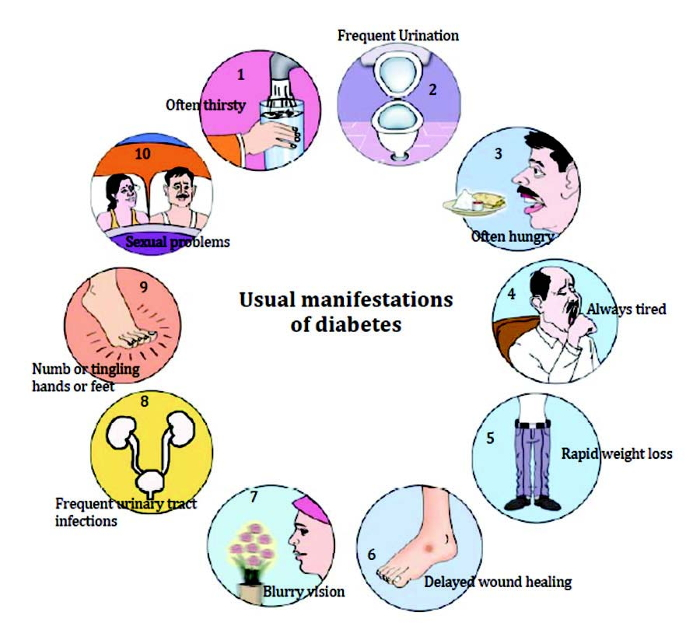
\includegraphics{images/023.jpg}
\caption{ಸರ್ವಾಂಗಾಸನ }
\end{figure}

\textbf{ \general{\enginline{1,}} ಸರ್ವಾಂಗಾಸನ:} ಈ ಆಸನವನ್ನು ಆರಂಭಿಸುವ ಮೊದಲು ನೆಲದ ಮೇಲೆ ಒಂದು ಜಮಖಾನೆಯನ್ನು ಹಾಕಿ ಅದರ ಮೇಲೆ ಅಂಗಾತ ಮಲಗಬೇಕು. ನಂತರ ನಿಧಾನವಾಗಿ, ಕಾಲುಗಳನ್ನೆತ್ತುತ್ತ ಬೆನ್ನನ್ನು ಸಹ ಎತ್ತಿ ನೆಟ್ಟಗೆ ಹೆಗಲುಗಳ ಮೇಲೆ ಭಾರಹಾಕಿ ತಲೆಕೆಳಗಾಗಿ, ಕಾಲು ಮೇಲಾಗಿ ನಿಲ್ಲಬೇಕು. ಈ ಸ್ಥಿತಿಯಲ್ಲಿ ದೇಹ ಭಾರವು ಸರಿಯಾಗಿ ನಿಲ್ಲುವಂತೆ ಎರಡೂ ಮುಂಗೈಗಳಿಂದ ಬೆನ್ನಬದಿಗಳನ್ನು ಹಿಡಿದುಕೊಳ್ಳಬೇಕು. ಭುಜಗಳು ನೆಲದ ಮೇಲಿದ್ದು ದೇಹ ನೆಟ್ಟಗಾಗಿರಲು ಸಹಾಯಕವಾಗಬೇಕು. ಗಡ್ಡದ ತುದಿಯು ಎದೆಗೆ ತಾಗಿಕೊಂಡಿರಬೇಕು. ಕಾಲುಗಳು ನೆಟ್ಟಗೆ ಮೇಲಕ್ಕಿರಬೇಕು. ಈ ತರದ ಸರ್ವಾಂಗಾಸನವನ್ನು ಆರಂಭಿಸಿದಾಗ, ಸಾಮಾನ್ಯ ಒಂದು ನಿಮಿಷ ಕಾಲ ಹಾಗೆಯೇ ನಿಲ್ಲಬೇಕು. ಬರಬರುತ್ತ ಅಭ್ಯಾಸವಾದ ಮೇಲೆ, ದೇಹದ ಶಕ್ತಿ ಮತ್ತು ಅವಶ್ಯಕತೆಗಳಿಗೆ ಅನುಗುಣವಾಗಿ ಒಂದರಿಂದ ಹತ್ತು ನಿಮಿಷಗಳವರೆಗೆ ಈ ಆಸನದಲ್ಲಿರಬೇಕು. ಸರ್ವಾಂಗಾಸನವು ಬಹುಮುಖ್ಯವಾದ ಆಸನವಾಗಿದೆ. ಇದು ದೇಹದ ಎಲ್ಲ ಅವಯವಗಳಲ್ಲೂ ಚುರುಕುತನವನ್ನುಂಟುಮಾಡಿ, ಮಾನವನಲ್ಲಿ ಆರೋಗ್ಯ ಮತ್ತು ಸಮತೋಲನವನ್ನುಂಟುಮಾಡಬಲ್ಲುದಾಗಿದೆ. ಇದು ನಿರ್ನಾಳ ಗ್ರಂಥಿಗಳ, ಅದರಲ್ಲೂ ಮುಖ್ಯವಾಗಿ ಥೈರಾಯ್ಡ್ ಮತ್ತು ಉಪಥೈರಾಯ್ಡ್ ಗ್ರಂಥಿಗಳ ಶಕ್ತಿಯನ್ನು ಹೆಚ್ಚಿಸಿ ಕಂಠ ಭಾಗದ ರಕ್ತಸಂಚಲನೆಯನ್ನು ತೀವ್ರಗೊಳಿಸುತ್ತದೆ. ಸರ್ವಾಂಗಾಸನವನ್ನು ನಿತ್ಯ ಮಾಡಿಕೊಂಡು ಬರುತ್ತಿರುವ ಸ್ವಯಂಸೇವಕರ ಜೀವ ರಾಸಾಯನಿಕ ಪರಿಶೀಲನೆ ಗೈದಾಗ, ಮೇಲೆ ಹೇಳಿದಂಶ ಸಂಪೂರ್ಣ ಸರಿಯೆಂದು ಕಂಡುಬಂದಿದೆ.

ಆರು ತಿಂಗಳ ಕಾಲ, ಸರಿಯಾದ ಸರ್ವಾಂಗಾಸನ ಹಾಗೂ ಇತರ ಆಸನಗಳನ್ನು ನಡೆಸಿಕೊಂಡು ಬಂದ ನಮ್ಮ ಸ್ವಯಂಸೇವಕರ ಪರೀಕ್ಷೆ ನಡೆಸಲಾಯಿತು. ಅವರ ಥೈರಾಯ್ಡ್ ನಾಳದ ಶಕ್ತಿಸೂಚಕವಾದ \enginline{PBI} ದ್ರವ \enginline{4.5 Meg} ಇದ್ದುದು \enginline{6.2 Meg} ಗೆ ಏರಿಬಂದುದನ್ನು ನಾವು ಕಂಡುಕೊಂಡಿದ್ದೇವೆ. ಸಾಮಾನ್ಯವಾಗಿ ಥೈರಾಯ್ಡ್ ಮತ್ತಿತರ ಗ್ರಂಥಿಗಳು ಸರಿಯಾಗಿ ಕೆಲಸ ಮಾಡದಿದ್ದಲ್ಲಿ ಜೀವದ್ರವ್ಯ ಪರಿಣಾಮ ದಲ್ಲಿ ಕುಂದುಂಟಾಗುತ್ತದೆ. ಹಾಗೆಯೇ ಕ್ರಮೇಣ ದೇಹದ ಎಲ್ಲ ಅವಯವಗಳ ಶಕ್ತಿ ಕುಂದುತ್ತ ಬಂದು ವೃದ್ದಾಪ್ಯ ಲಕ್ಷಣ ತೋರಿಬರುತ್ತದೆ. ಅದಲ್ಲದೆ ಈ ಆಸನಸ್ಥಿತಿಯಲ್ಲಿರುವಾಗ ದೇಹದ ಕೆಳಭಾಗದ ರಕ್ತನಾಳಗಳಲ್ಲಿ ಹಾಗೂ ಜಠರ ಮತ್ತು ಕರುಳಲ್ಲಿ ರಕ್ತಸಂಚಾರ ಹೆಚ್ಚಾಗಿ ಹೃದಯದವರೆಗಿನ ಎಲ್ಲ ಅವಯವಗಳ ಶಕ್ತಿಯೂ ಹೆಚ್ಚುವಂತಾಗುತ್ತದೆ.

ಇಷ್ಟೇ ಅಲ್ಲದೆ ಜೀವನಾಧಾರವಾದ ಜಠರದ ಶಕ್ತಿಯೂ ಹೆಚ್ಚಿ, ಒಳ್ಳೆಯ ಹಸಿವು, ಸರಿಯಾದ ಮಲಶೋಧನೆ ಒದಗಿಬರುತ್ತವೆ. ಈ ಸರ್ವಾಂಗಾಸನದ ಸ್ಥಿತಿಯಿಂದಾಗಿ ಹೃದಯ, ಶ್ವಾಸಕೋಶ ಮತ್ತು ಮಿದುಳುಗಳಲ್ಲಿ ಗುರುತ್ವಾಕರ್ಷಣ ಶಕ್ತಿಯಿಂದ ರಕ್ತಸಂಚಾರವು ಹೆಚ್ಚಾಗುತ್ತದೆ. ಇದರಿಂದ ಈ ಮರ್ಮಾಂಗಗಳ ಶಕ್ತಿ ಹೆಚ್ಚಿ ಅವು ಚುರುಕಾಗುತ್ತವೆ. ಇವನ್ನೆಲ್ಲ ಆರು ತಿಂಗಳಕಾಲ ಪ್ರತಿದಿನ ಸರ್ವಾಂಗಾಸನ ನಡೆಸಿಕೊಂಡು ಬಂದ ಸ್ವಯಂಸೇವಕರಲ್ಲಿ ನಾವು ಪರೀಕ್ಷಿಸಿಕೊಂಡಿದ್ದೇವೆ. ಹಾಗಾಗಿ ಇದು ಬಹುಮುಖ್ಯವಾದ ಆಸನವಾದ ಕಾರಣ, ಆರೋಗ್ಯಾಭಿಲಾಷಿಗಳಾದ ಎಲ್ಲರೂ ಮಾಡಲು ಕಲಿಯಬೇಕು, ಹಾಗೂ ನಿತ್ಯ ಅನುಸರಿಸಿಕೊಂಡು ಬರಬೇಕು.

\textbf{ \general{\enginline{2.}} ಮತ್ಸ್ಯಾಸನ:} ಈ ಆಸನದಲ್ಲಿ ಮೊದಲು ಪದ್ಮಾಸನ ಹಾಕಿ ಕುಳಿತುಕೊಂಡು ನಂತರ ನಿಧಾನವಾಗಿ ಮಲಗುವ ಸ್ಥಿತಿಗೆ ಬರಬೇಕು. ಹಾಗೆ ಮಲಗುವಾಗ ತಲೆ ಮತ್ತು ಸೊಂಟ ಮಾತ್ರ ನೆಲಕ್ಕೆ ಮುಟ್ಟಿಕೊಂಡಿರಬೇಕು. ಬೆನ್ನು ಕಮಾನಿನಂತೆ

\begin{figure}
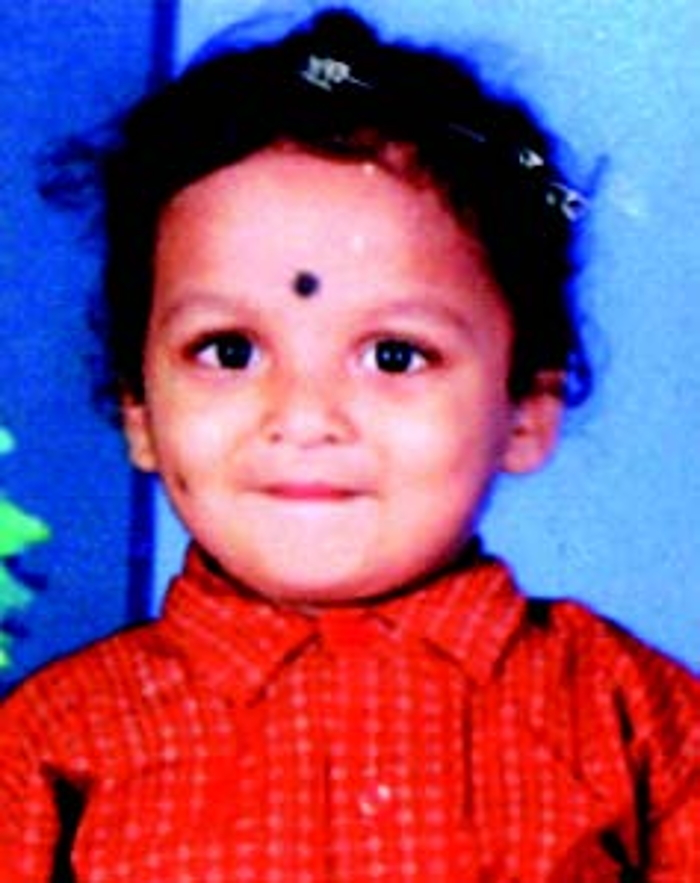
\includegraphics{images/024.jpg}
\caption{\textbf{ಮತ್ಸ್ಯಾಸನ} }
\end{figure}

ಬಾಗಿಕೊಂಡಿರಬೇಕು. ಕೈಬೆರಳುಗಳು ಕಾಲ್ಬೆರಳುಗಳನ್ನು ಹಿಡಿದಿರಬೇಕು. ದೀರ್ಘಶ್ವಾಸವನ್ನು ಒಳಕ್ಕೆ ತೆಗೆದುಕೊಂಡು ಅಲ್ಲೇ ಧಾರಣಗೈದು ನಂತರ ನಿಧಾನವಾಗಿ ಹೊರಬಿಡಬೇಕು. ಈ ತರದ ಮತ್ಸ್ಯಾಸನವನ್ನು ಒಂದರಿಂದ ಮೂರು ನಿಮಿಷಗಳ ತನಕ ಗೈಯಬೇಕು. ಈ ಆಸನಾಭ್ಯಾಸದಿಂದ ಜಠರ ಸಂಬಂಧವಾದ ಎಲ್ಲ ಅವಯವಗಳೂ ಚುರುಕುಗೊಳ್ಳುತ್ತವೆ. ಶ್ವಾಸೋಚ್ಛ್ವಾಸ ವಿಧಾನವೂ ಬಲಗೊಳ್ಳುತ್ತದೆ. ಥೈರಾಯ್ಡ್ ಗ್ರಂಥಿಯ ಶಕ್ತಿ ಸಹ ಹೆಚ್ಚಿನ ರಕ್ತಸಂಚಾರದಿಂದಾಗಿ ಚುರುಕುಗೊಂಡು ಅದು ಪುನರ್ನವೀಕೃತವಾಗುತ್ತದೆ. ಸರ್ವಾಂಗಾಸನದ ನಂತರ ಈ ಆಸನವನ್ನು ನಡೆಸುವುದು ಉತ್ತಮ.

\textbf{ \general{\enginline{3.}} ಪಶ್ಚಿಮೋತ್ಥಾನಾಸನ:} ಈ ಆಸನದಲ್ಲಿ ನಾವು ಮೊದಲು ನೆಲದ ಮೇಲೆ ಅಂಗಾತ ಮಲಗಿಕೊಳ್ಳಬೇಕು. ನಂತರ ನಿಧಾನವಾಗಿ ದೇಹದ ಊರ್ಧ್ವಭಾಗವನ್ನು

\begin{figure}
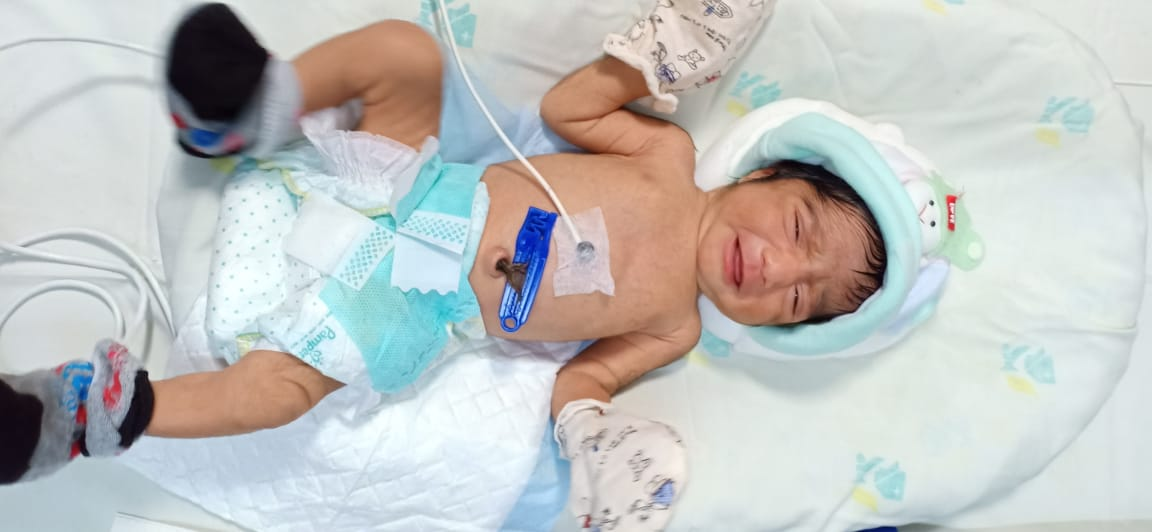
\includegraphics{images/025.jpg}
\caption{\textbf{ಪಶ್ಚಿಮೋತ್ಥಾನಾಸನ} }
\end{figure}

ಎತ್ತುತ್ತ ಬರಬೇಕು. ಹಾಗೆಯೇ ಮುಂದುವರಿದು ಚಾಚಿದ ನೆಟ್ಟಗಿರುವ ಕಾಲುಗಳಿಗೆ ತಲೆಯನ್ನು ಮುಟ್ಟಿಸಬೇಕು. ಮೊಣಕಾಲ ಗಂಟು ಬಾಗಬಾರದು. ಮುಖವು ಎರಡು ಮೊಣಗಂಟುಗಳ ಮಧ್ಯದಲ್ಲಿರಬೇಕು. ಈ ಸ್ಥಿತಿಯಲ್ಲಿ ಒಂದರಿಂದ ಮೂರು ನಿಮಿಷಗಳವರೆಗಿರಬೇಕು. ಇದರಿಂದ ಜಠರದ ಎಲ್ಲ ಸ್ನಾಯುಗಳಿಗೂ ಬಲ ಒದಗಿಬರುತ್ತದೆ. ಹಾಗೆಯೇ ಜಠರದ ಕೆಳಭಾಗದಲ್ಲಿರಬಹುದಾದ ಎಲ್ಲ ತರದ ವಾಯುವೂ \enginline{(Gas)} ಹೊರದೂಡಲ್ಪಡುತ್ತದೆ. ಅಷ್ಟೇ ಅಲ್ಲದೆ ಬೆನ್ನುಮೂಳೆಯ ಸ್ನಾಯು ಹಾಗೂ ಅಸ್ಥಿರಜ್ಜು \enginline{(Ligaments)} ವಿನ ಶಕ್ತಿ ವೃದ್ಧಿಯಾಗುತ್ತದೆ. ರಕ್ತಸಂಚಾರ ಹೆಚ್ಚಿ ಬೆನ್ನು ಹುರಿಯ ಸಾಮರ್ಥ್ಯ ಚುರುಕಾಗುತ್ತದೆ.

\textbf{ \general{\enginline{4.}} ಹಲಾಸನ:} ಹಲ ಎಂದರೆ ನೇಗಿಲು, ದೇಹವನ್ನು ನೇಗಿಲಾಕಾರದಲ್ಲಿ ಬಗ್ಗಿಸುವುದೇ ಹಲಾಸನ. ಈ ಆಸನದಲ್ಲಿ ನಾವು ಮೊದಲು ನೆಲದ ಮೇಲೆ ಅಂಗಾತ (ಬೆನ್ನು ಕೆಳಗಾಗಿ) ಮಲಗಬೇಕು. ನಂತರ ಕ್ರಮೇಣ ಕಾಲು ಮತ್ತು ಬೆನ್ನನ್ನು ಎತ್ತಿ ಹಿಂದಕ್ಕೆ ಬಾಗಿಸಬೇಕು. ಆಮೇಲೆ ನಿಧಾನವಾಗಿ ಕಾಲ ಹೆಬ್ಬೆರಳು, ತಲೆ ದಾಟಿ ಹೋಗಿ ನೆಲ ಮುಟ್ಟಬೇಕು. ಎರಡು ಭುಜಗಳನ್ನು ನೆಟ್ಟಗೆ ನೆಲದ ಮೇಲೆ ಚಾಚಬೇಕು. ಈ ಆಸನಗೈಯುವಾಗ ಕಾಲು ಮತ್ತು ಕಾಲಗಂಟು ಗಟ್ಟಿಯಾಗಿದ್ದು ಬಾಗದೆ ನೆಟ್ಟಗಾಗಿರಬೇಕು. ಈ ಆಸನವನ್ನು ನಿಧಾನವಾಗಿ ಮಾಡಬೇಕು. ವಯಸ್ಸಾ ದವರು ಈ ಆಸನಗೈಯುವಾಗ ಬೆನ್ನು ಮತ್ತು ಕುತ್ತಿಗೆಯ ಸ್ನಾಯುಗಳಿಗೆ ನೋವುಂಟಾಗದಂತೆ ಸಾವಕಾಶವಾಗಿರಬೇಕು. ಈ ಸ್ಥಿತಿಯಲ್ಲಿ ಸಾಮಾನ್ಯ ಒಂದರಿಂದ ಐದು ನಿಮಿಷಗಳವರೆಗಿರಬೇಕು ಈ ಆಸನದಿಂದ ಬೆನ್ನೆಲುಬಿಗೆ ಉತ್ತಮ ವ್ಯಾಯಾಮ ದೊರಕುತ್ತದೆ. ಜಠರದಲ್ಲಿರುವ ಕರುಳಿನ ನಾಳದ ಚಟುವಟಿಕೆ ಚುರುಕಾಗುತ್ತದೆ. ವಾಯು ತುಂಬಿದ ದೊಡ್ಡ ಕರುಳಿನ ನಿರ್ಮಲೀಕರಣವಾಗಿ ದೇಹ ಮನಸ್ಸುಗಳಿಗೆ ನೆಮ್ಮದಿ ದೊರಕುತ್ತದೆ.

\begin{figure}

\includegraphics{images/026.jpg}
\caption{\textbf{ಹಲಾಸನ} }
\end{figure}

\textbf{ \general{\enginline{5.}} ಭುಜಂಗಾಸನ:} ಭುಜಂಗ ಅಂದರೆ ಸರ್ಪ. ಸರ್ಪದ ಹೆಡೆ ಎತ್ತಿರುವಂತೆ ನಡೆಸುವ ಆಸನವೇ ಭುಜಂಗಾಸನ. ಈ ಆಸನದಲ್ಲಿ ನಾವು ನೆಲದ ಮೇಲೆ ಮುಖ ಕೆಳಗಾಗಿ ಮೊದಲು ಮಲಗಬೇಕು. ಆಮೇಲೆ ನಾಭಿಯಿಂದ ಮೇಲಿನ ದೇಹ ಭಾಗವನ್ನು ನಿಧಾನವಾಗಿ ಮೇಲಕ್ಕೆತ್ತಿ ಹಿಂದೆ ಬಾಗಿಸಬೇಕು. ದೇಹದ ಭಾರವೆಲ್ಲ ಕೈ ಮತ್ತು ಭುಜಗಳ ಮೇಲೆ ಬೀಳುವಂತಾಗಬೇಕು. ನಂತರ ತಲೆ, ಕುತ್ತಿಗೆ, ಎದೆ– ಎಲ್ಲವನ್ನೂ ಸಾಧ್ಯವಾದ ಮಟ್ಟಿಗೆ ಹಿಂದಕ್ಕೆ ಬಗ್ಗಿಸಬೇಕು. ನೋಡುವಾಗ ಹೆಡೆ ಎತ್ತಿ ಕೆರಳಿ ನಿಂತ ಭುಜಂಗದಂತೆ ತೋರಬೇಕು. ಈ ಸ್ಥಿತಿಯಲ್ಲಿ ಒಂದೆರಡು ನಿಮಿಷ ಇರಬೇಕು. ಇದರಿಂದ ಬೆನ್ನ ಮೂಳೆಯ ಎಲ್ಲ ತರದ ನೋವು ದೂರವಾಗಿ ದೇಹಶಕ್ತಿ ಹೆಚ್ಚಿಬರಲು ಅನುಕೂಲವಾಗುತ್ತದೆ. ಎದೆ ಅಗಲವಾಗಿ ದೇಹಸೌಷ್ಟವು ಹೆಚ್ಚಲು ಕಾರಣವಾಗುತ್ತದೆ.

\begin{figure}
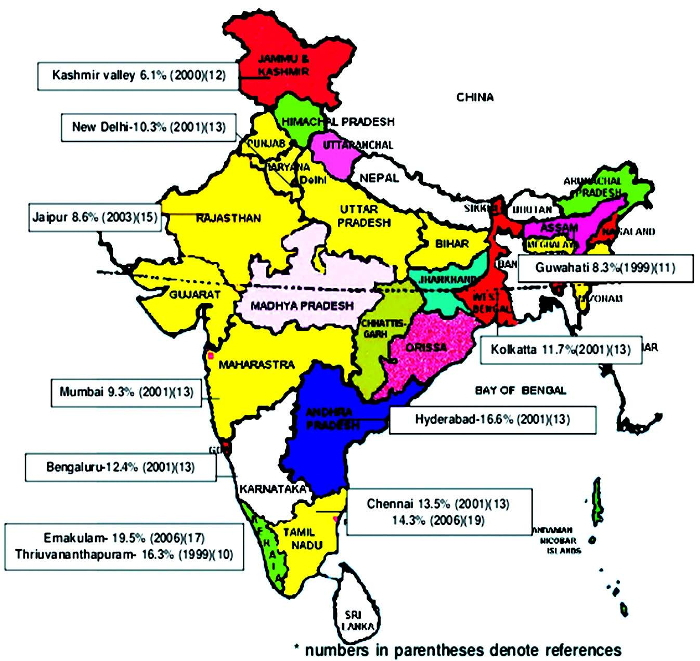
\includegraphics{images/027.jpg}
\caption{\textbf{ಭುಜಂಗಾಸನ} }
\end{figure}

\textbf{ \general{\enginline{6.}} ಶಲಭಾಸನ:} ಈ ಆಸನ ಮಾಡುವಾಗ ಮೊದಲು ಮುಖ ಕೆಳಗಾಗಿ ಮಲಗಬೇಕು. ನಂತರ ನಿಧಾನವಾಗಿ ಕಾಲುಗಳನ್ನು ಮೇಲಕ್ಕೆತ್ತಬೇಕು. ಕಾಲ ಗಂಟು ಸ್ವಲ್ಪವೂ ಬಾಗಬಾರದು. ಆಗ ದೇಹದ ಊರ್ಧ್ವಭಾಗವನ್ನು ಗಡ್ಡ ಸಹಿತ ನೆಲದಮೇಲೆಯೇ ಇಟ್ಟಿರಬೇಕು. ಎರಡೂ ಬಾಹುಗಳನ್ನು ದೇಹಕ್ಕೊತ್ತಾಗಿ ನೆಲದ ಮೇಲಿಟ್ಟು ದೇಹದ ಭಾರ ತಡೆದುಕೊಳ್ಳುವುದಕ್ಕೆ ಆಧಾರವಾಗಿಡಬೇಕು. ಅನಂತರ ನಿಧಾನವಾಗಿ ದೇಹದ ಊರ್ಧ್ವಭಾಗವನ್ನೂ ಎತ್ತಿ ಹಿಂದಕ್ಕೆ ಸಾಧ್ಯವಾದಷ್ಟು ಕುತ್ತಿಗೆ ಸಹಿತ ಬಾಗಿಸಬೇಕು. ಮೊದಮೊದಲು ಈ ಆಸನ ಸಾಧನೆ ಕಷ್ಟವಾಗಿ ಕಾಣಬಹುದು.ಆದರೆ ಅಭ್ಯಾಸ ಮಾಡುತ್ತಾ, ಅದರಲ್ಲೂ ಮೊದಲು ಒಂದೊಂದೇ ಕಾಲನ್ನೆತ್ತಿ ಬಾಗಿಸುತ್ತ ರೂಢಿಗೊಳಿಸಿಕೊಂಡರೆ ಸರಿಹೋಗುತ್ತದೆ. ಬೆನ್ನೆಲುಬು, ಬೆನ್ನುಹುರಿಯ ಸ್ನಾಯುಗಳಿಗೆ ಬಲ ಬರುವುದಕ್ಕೆ ಅನುಕೂಲವಾಗುವ ಈ ಆಸನವನ್ನು ಸಾಮಾನ್ಯ ಒಂದು ನಿಮಿಷದವರೆಗೆ, ಒಮ್ಮೆಗೆ ಸಾಧಿಸಿಕೊಂಡು ಬರಬಹುದು. ಹೊಟ್ಟೆಯ ಸ್ನಾಯುವಿಗೆ ಸಹ ಒಳ್ಳೆಯ ಶಕ್ತಿಯನ್ನುಂಟುಮಾಡುವ ಈ ಆಸನ ಮಧ್ಯ ವಯಸ್ಸಿನ ಪುರುಷರಿಗೂ ಸ್ತ್ರೀಯರಿಗೂ ತುಂಬ ಉಪಕಾರಿಯಾಗುತ್ತದೆ.

\begin{figure}
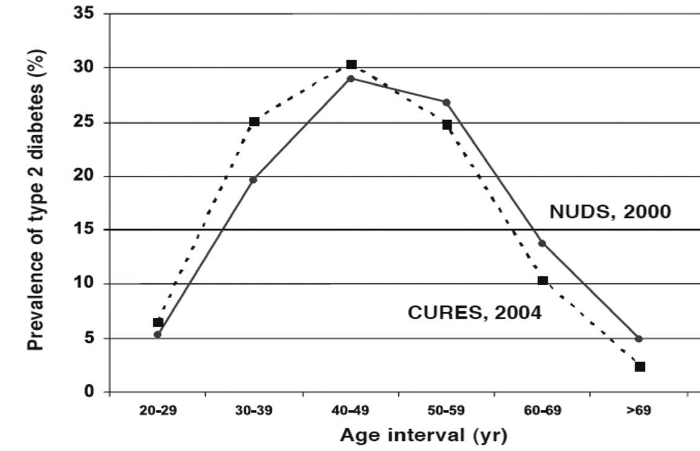
\includegraphics{images/028.jpg}
\caption{\textbf{ಶಲಭಾಸನ} }
\end{figure}

\textbf{ \general{\enginline{7.}} ಅರ್ಧಮತ್ಸೇಂದ್ರಾಸನ:} ಈ ಆಸವನ್ನಾರಂಭಿಸುವಾಗ ನೆಲದ ಮೇಲೆ ದೃಢವಾಗಿ ಕುಳಿತು ಎಡಗಾಲ ಹಿಮ್ಮಡಿಯನ್ನ ಗುದಭಾಗದ ಕೆಳಗಿಟ್ಟುಕೊಳ್ಳಬೇಕು. ಬಲಪಾದವನ್ನು ಎಡಗಾಲ ಗಂಟಿನ ಹತ್ತಿರ, ಮೇಲಿಂದ ತಂದು ಬಲಕಾಲ ಮೊಣ ಗಂಟನ್ನು ಮೇಲಕ್ಕೆತ್ತಿ ನೆಲದ ಮೇಲಿಡಬೇಕು. ಹಾಗೆ ಎತ್ತಿದ ಬಲಕಾಲ ಮೊಣ ಗಂಟನ್ನು ಎಡಕಂಕುಳ ಅಡಿಯಲ್ಲಿರಿಸಬೇಕು. ನಂತರ ಬೆನ್ನನ್ನು ಬಲಕ್ಕೆ ತಿರುಗಿಸಿ ಮುಖ ಮತ್ತು ಭುಜ ಒಂದೇ ಸಮರೇಖೆಯಲ್ಲಿರುವಂತೆ ಮಾಡಬೇಕು. ಬಲತೋಳು ಬೆನ್ನ ಹಿಂದಿನಿಂದ ಸುತ್ತಿಕೊಂಡುಹೋಗಿ ಎಡತೊಡೆಯನ್ನು ಹಿಡಿದುಕೊಳ್ಳಬೇಕು. ಈ ತರದ ಆಸನವನ್ನು ಎಡಗಾಲಿಂದ ಆರಂಭಿಸಿದ ಹಾಗೆಯೇ ಬಲಗಾಲಿಂದಾರಂಭಿಸಿ ನಡೆಸಬೇಕು. ಇದರಿಂದ ಎರಡೂ ಪಾರ್ಶ್ವಗಳಿಗೆ ಈ ಆಸನದ ಪ್ರಯೋಜನ ದೊರಕುತ್ತದೆ. ಈ ಆಸನವನ್ನು ನಿತ್ಯ ನಡೆಸುವುದರಿಂದ ಮಲಶುದ್ಧಿ ಉಂಟಾಗಿ ಮೂತ್ರಕೋಶದ ಸ್ನಾಯುಗಳಿಗೆ ಶಕ್ತಿ ಬರುವಂತಾಗುತ್ತದೆ. ಗುದದ್ವಾರ ಮೂತ್ರ ನಾಳಗಳೂ ಶುದ್ಧವಾಗುತ್ತವೆ.

\begin{figure}
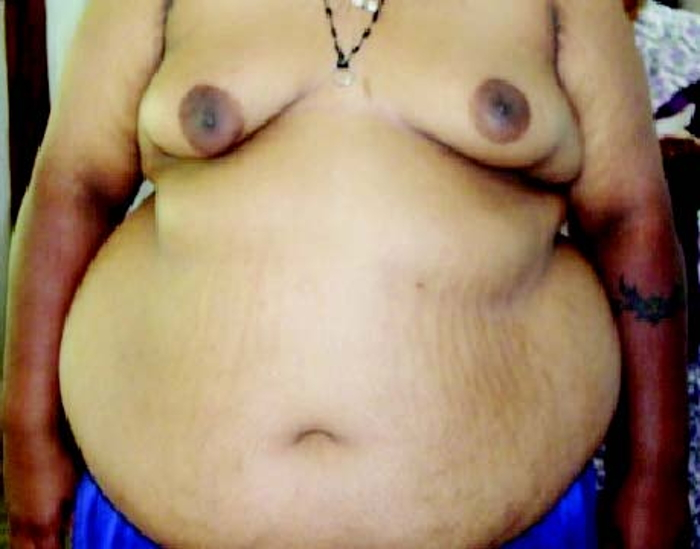
\includegraphics{images/029.jpg}
\caption{\textbf{ಅರ್ಧಮತ್ಸೇಂದ್ರಾಸನ} }
\end{figure}

\textbf{ \general{\enginline{8.}} ಮಯೂರಾಸನ:} ಈ ಆಸನ ಮಾಡುವಾಗ ಮೊದಲು ಮುಖ ಕೆಳಗಾಗಿ ಮಲಗಬೇಕು. ನಂತರ ಸೊಂಟದಿಂದ ಮೇಲಿನ ದೇಹವನ್ನೆತ್ತಿಕೊಂಡು ಮೊಣಕಾಲ ಗಂಟಿನ ಮೇಲೆ ಕುಳಿತುಕೊಳ್ಳಬೇಕು. ಆಮೇಲೆ ಮುಂದಕ್ಕೆ ಬಾಗಿ ತನ್ನ ಎರಡೂ ಅಂಗೈಗಳನ್ನು ಪಾದಾಭಿಮುಖವಾಗಿ ನೆಲದ ಮೇಲಿಡಬೇಕು. ನಂತರ ಮುಂಗೈಯನ್ನು ಬಾಗಿಸಿ ಒಟ್ಟಾಗಿಸಿ ಆ ಎರಡು ಮುಂಗೈಗಳ ಮೇಲೆ ದೇಹಭಾರ ಬೀಳುವಂತೆ ಎರಡೂ ಕಾಲುಗಳನ್ನೆತ್ತಿ, ನೆಟ್ಟಗೆ ಮೇಲಕ್ಕೆ ಎತ್ತಿಕೊಳ್ಳಬೇಕು. ಭೂಮಿಗೆ ಸಮಾನಾಂತರ ರೇಖೆಯಲ್ಲಿ ಮುಂದೆ ನೋಡಿಕೊಂಡು ದೇಹಭಾರ ಸಮತೂಕದಲ್ಲಿರುವಂತೆ ನೋಡಿಕೊಳ್ಳಬೇಕು. ಈ ಸ್ಥಿತಿಯನ್ನು ಕೆಲವು ಸೆಕೆಂಡುಗಳಿಂದ ಆರಂಭಿಸಿ ಕ್ರಮೇಣ ಎರಡು ನಿಮಿಷಗಳವರೆಗೆ ಧರಿಸಿಕೊಂಡಿರಬಹುದು. ಇದರಿಂದ ಜಠರದ ಸ್ನಾಯುಗಳಿಗೆ ಶಕ್ತಿ ಬರುವುದು ಮಾತ್ರವೇ ಅಲ್ಲ; ಜಠರ ಮತ್ತು ಕರುಳಿನ ಅತಿಸೂಕ್ಷ್ಮ ಸ್ನಾಯುಗಳು ಸಹ ಚುರುಕುಗೊಂಡು ಹಸಿವು ಹೆಚ್ಚಾಗಿ ಜೀರ್ಣಶಕ್ತಿ ಬಲಗೊಳ್ಳುತ್ತದೆ. ಮಧುಮೇಹದಿಂದ ಬಳಲಿಕೊಂಡಿರುವವರು ಈ ಆಸನಾಭ್ಯಾಸ ಮಾಡುವುದರಿಂದ ರಕ್ತದ ಶರ್ಕರಾಂಶವನ್ನು ಕುಗ್ಗಿಸಲು ಸಮರ್ಥರಾಗಬಹುದು. ಅಷ್ಟೇ ಅಲ್ಲದೆ ಭುಜ, ಮುಂಗೈ ಮಣಿಗಂಟುಗಳ ಸ್ನಾಯುಗಳೂ ಬಲಗೊಳ್ಳುತ್ತವೆ.

\begin{figure}
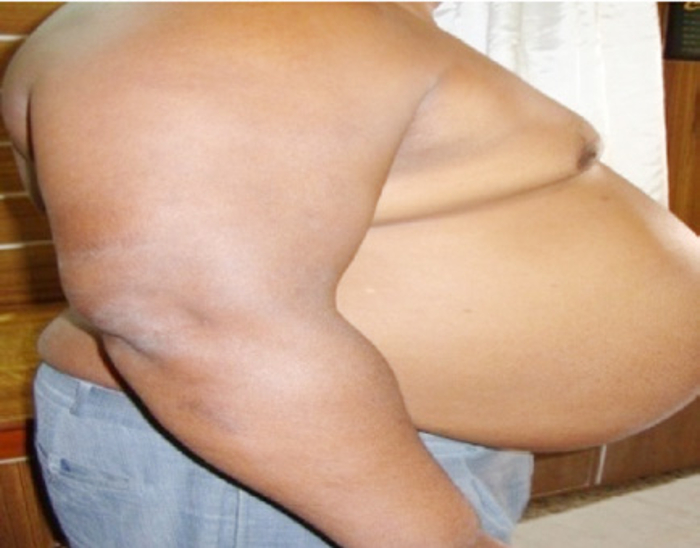
\includegraphics{images/030.jpg}
\caption{\textbf{ಮಯೂರಾಸನ} }
\end{figure}

\textbf{ \general{\enginline{9.}} ಧನುರಾಸನ:} ಈ ಆಸನಗೈಯುವಾಗ ಮೊದಲು ನಾವು ಮುಖ ಕೆಳಮಾಡಿ ಉದ್ದಕ್ಕೆ ಮಲಗಬೇಕು. ಕಾಲು ಮತ್ತು ಪಾದಗಳನ್ನು ಒತ್ತಾಗಿ ಜೋಡಿಸಿಡಬೇಕು. ನಂತರ ನಿಧಾನವಾಗಿ ಕಾಲನ್ನು ನೆಟ್ಟಗೆ ಮೇಲೆತ್ತಬೇಕು. ಇನ್ನೊಂದೆಡೆಯಿಂದ ತಲೆ, ಮುಖ, ಎದೆಗಳನ್ನು ಎತ್ತಿಕೊಳ್ಳುತ್ತ ದೇಹಭಾರವೆಲ್ಲ ಹೊಟ್ಟೆಯ ಮೇಲೆ ಬೀಳುವಂತೆ ಮಾಡಬೇಕು. ಹಾಗೆ ಎರಡೂ ಕಡೆಯಿಂದ ಎತ್ತಿದ ದೇಹ ಭಾಗಗಳನ್ನು, ಕೈಯನ್ನು ಹಿಂದಕ್ಕೆ ಸರಿಸಿ ಪಾದದ ಗಂಟನ್ನು ಹಿಡಿದುಕೊಂಡು ಧನುಸ್ಸಿನಾಕಾರಕ್ಕೆ ತರಬೇಕು. ಈ ಸ್ಥಿತಿಯಲ್ಲಿ ಸ್ವಲ್ಪ ಸಮಯ ಮಾತ್ರ ಇರಲು ಸಾಧ್ಯವಾಗಬಹುದು. ಇದರಿಂದ ಬೆನ್ನಹುರಿಯನ್ನು ಇಷ್ಟಬಂದಂತೆ ಬಾಗಿಸುವ ಸಾಮರ್ಥ್ಯವನ್ನು ಗಳಿಸಿಕೊಳ್ಳಬಹುದು. ಹಾಗೆಯೇ ಜಠರದ ಸ್ನಾಯುಗಳಿಗೆ ಶಕ್ತಿಯನ್ನೂ ಒದಗಿಸಬಹುದು.

\begin{figure}
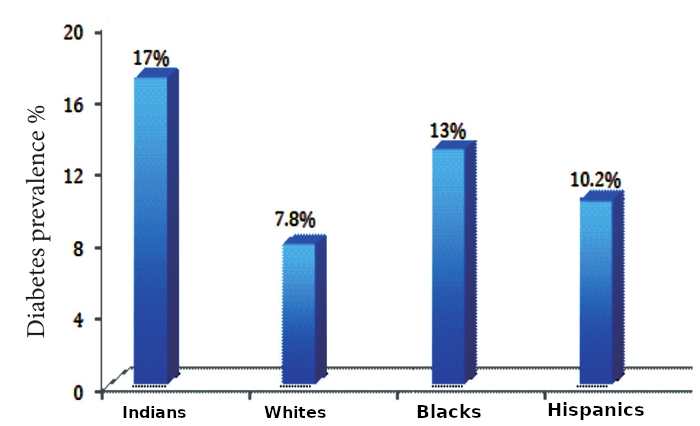
\includegraphics{images/031.jpg}
\caption{\textbf{ಧನುರಾಸನ} }
\end{figure}

\textbf{ \general{\enginline{10.}} ಶೀರ್ಷಾಸನ:} ತಲೆ ಕೆಳಗಾಗಿ ನಿಲ್ಲುವ ಈ ಆಸನವು ಅತಿ ಮುಖ್ಯವಾದ ಆಸನಗಳಲ್ಲೊಂದಾಗಿದೆ. ಈ ಆಸನದಲ್ಲಿ ಇಡೀ ದೇಹದ ಭಾರ ತಲೆಯ ಮೇಲೆ ಬೀಳುವುದರಿಂದ ಬರಿ ತಲೆಯನ್ನು ನೆಲದ ಮೇಲಿಟ್ಟಾಗ ನೋವಾಗುವುದು ಸಹಜ. ಅದಕ್ಕಾಗಿ ತಲೆಯಡಿಯಲ್ಲಿ ಒಂದು ದಿಂಬು ಅಥವಾ ನಾಲ್ಕಾರು ಪದರು ಮಡಚಿದ ಬಟ್ಟೆಯನ್ನಿಟ್ಟುಕೊಳ್ಳುವುದು ಅಗತ್ಯ. ಅಥವಾ ಎರಡೂ ಕೈಗಳ ಬೆರಳುಗಳನ್ನು ಹೆಣೆದುಕೊಂಡು ಅದರ ಮೇಲೆ ತಲೆ ಇಟ್ಟುಕೊಳ್ಳಲೂ ಬಹುದು.

\begin{figure}
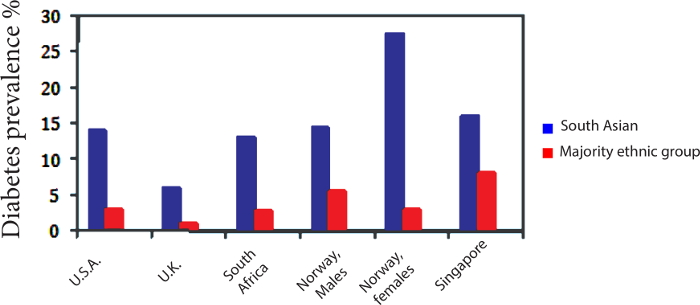
\includegraphics{images/032.jpg}
\caption{\textbf{ಶೀರ್ಷಾಸನ} }
\end{figure}

ಈ ಆಸನ ಆರಂಭಿಸುವಾಗ, ಮೊತ್ತ ಮೊದಲು ನೆಲದ ಮೇಲೆ ಮೊಣಕಾಲು ಊರಿ ಕುಳಿತುಕೊಳ್ಳಬೇಕು. ನಂತರ ಮುಂದಕ್ಕೆ ಬಾಗಿ ಮುಂಗೈ ಮತ್ತು ತಲೆಯನ್ನು ನೆಲದ ಮೇಲಿಡಬೇಕು. ಆಮೇಲೆ ಕಾಲು ಮತ್ತು ಸೊಂಟವನ್ನು ಮೇಲಕ್ಕೆತ್ತಿ ನಿಧಾನವಾಗಿ ತಲೆಕೆಳಗಾಗಿ ನಿಲ್ಲಬೇಕು. ಮೊದಮೊದಲು ಅಭ್ಯಾಸವಾಗುವವರೆಗೆ ಇನ್ನೊಬ್ಬರ ಸಹಾಯ ಅಥವಾ ಗೋಡೆಯ ಮೂಲೆಯ ಸಹಾಯ ಪಡೆದುಕೊಳ್ಳಬಹುದು. ಅಭ್ಯಾಸವಾದ ಮೇಲೆ ಯಾವ ಸಹಾಯವೂ ಇಲ್ಲದೆ ಈ ಆಸನವನ್ನು ಸಾಧಿಸಿಕೊಳ್ಳಲಾಗುತ್ತದೆ. ಸಾಧಾರಣವಾಗಿ ಈ ಸ್ಥಿತಿಯಲ್ಲಿ ಐದು ನಿಮಿಷಗಳವರೆಗೆ ಇರುವುದು ಹಿತಕರ. ಆದರೆ ಕೆಲವರು ಅದಕ್ಕಿಂತಲೂ ಹೆಚ್ಚಿನ ಸಮಯ ತಲೆಕೆಳಗಾಗಿರುವವರು ಇದ್ದಾರೆ. ಆದರೆ ಹೆಚ್ಚಿನ ಸಮಯದ ವ್ಯಯದಿಂದ ಹೆಚ್ಚಿನ ಪ್ರಯೋಜನ ಆದಂತಿಲ್ಲ. ಆದರೆ ಶೀರ್ಷಾಸನ ಮಾಡಿದ ನಂತರ ತುಂಬಾ ಹೊಸತನ ತೋರಿಬರುತ್ತದೆಂದು ವೈಯಕ್ತಿಕಾನುಭವವನ್ನು ಹೆಚ್ಚಿನವರು ಹೇಳುತ್ತಾರೆ ಇದು ಮಿದುಳಿಗೆ ಹೆಚ್ಚಾದ ರಕ್ತಸಂಚಾರ ಹಾಗೂ ಗುರುತ್ವಾಕರ್ಷಣದ ಬದಲಾವಣೆಯಿಂದಾಗಿ ತೋರಿ ಬಂದಿರಬೇಕು.

ಇದು ಮಿದುಳಿನ ನರನಾಡಿಗಳ ಸವೆತ ಕಡಿಮೆಯಾಗುವುದಕ್ಕೆ ಸಹಕಾರಿಯಾಗಿ ಮಿದುಳಿನ ಸಾಮರ್ಥ್ಯವನ್ನು ಹೆಚ್ಚಿಸುತ್ತದೆ. ಹಾಗಾಗಿ ಕ್ರಮಪ್ರಕಾರ ಪ್ರತಿದಿನ ಮಾಡುವ ಶೀರ್ಷಾಸನವು ಮಿದುಳ ಮೂಲದ ಪಿಟ್ಯುವಿಟರಿ ಮತ್ತು ಪೈನಿಯಲ್ ನಿರ್ನಾಳ ಗ್ರಂಥಿಗಳ ಶಕ್ತಿಯನ್ನು ಹೆಚ್ಚಿಸಿ ಜ್ಞಾಪಕಶಕ್ತಿ ಮತ್ತು ಮನಸ್ಸಿನ ಏಕಾಗ್ರತಾ ಶಕ್ತಿಯನ್ನು ಉತ್ತಮಪಡಿಸುತ್ತದೆ. ಆದಕಾರಣ ಜ್ಞಾಪಕಶಕ್ತಿ ಹಾಗೂ ಉತ್ಸಾಹ ಕುಂದಿ ಕುಗ್ಗಿ ಹೋದವರಿಗೆ ಈ ಆಸನ ತುಂಬ ಉಪಕಾರಿಯಾಗಬಹುದು. ಮಿದುಳಿಗೆ ಸಂಬಂಧಪಟ್ಟ ಕಾಯಿಲೆಗಳಿಂದ ನರಳುತ್ತಿರುವರು ಸಹ ಸುಧಾರಣೆ ಪಡೆದು ಚುರುಕಾಗುವ ಸಂಭವ ಬಹಳ ಇದೆ.

ಈ ವಿಷಯದಲ್ಲಿ ಯೋಗತಜ್ಞ ಶ‍್ರೀ ಅಯ್ಯಂಗಾರ್ ಅವರು 'ಶೀರ್ಷಾಸನವನ್ನು ಕ್ರಮಪ್ರಕಾರ ಮಾಡುತ್ತ ಬಂದರೆ ದೇಹ ಬೆಳೆಯುತ್ತದೆ; ಮನಸ್ಸು ಬುದ್ಧಿ ಶಿಸ್ತುಬದ್ಧವಾಗುತ್ತವೆ. ಮತ್ತು ಆತ್ಮಶಕ್ತಿ ವಿಕಾಸಗೊಳ್ಳುತ್ತದೆ. ಸುಖ–ದುಃಖ, ಲಾಭ–ನಷ್ಟ, ಮಾನ–ಅಪಮಾನ, ಜಯ–ಅಪಜಯಗಳು ಒದಗಿದಾಗ ಮಾನವನು ಸ್ಥಿತ ಪ್ರಜ್ಞನಾಗಿ ಶಾಂತನಾಗಿರಲು ಸಮರ್ಥನಾಗುತ್ತಾನೆ' ಎಂದಿದ್ದಾರೆ. ಆದರೂ ಸಹ, ರಕ್ತದ ಒತ್ತಡದ ಕಾಯಿಲೆಯವರು ಮತ್ತು ವಯಸ್ಸಾದವರು ಈ ಆಸನವನ್ನು ಮಾಡದಿರುವುದು ಒಳ್ಳೆಯದು.

\begin{figure}
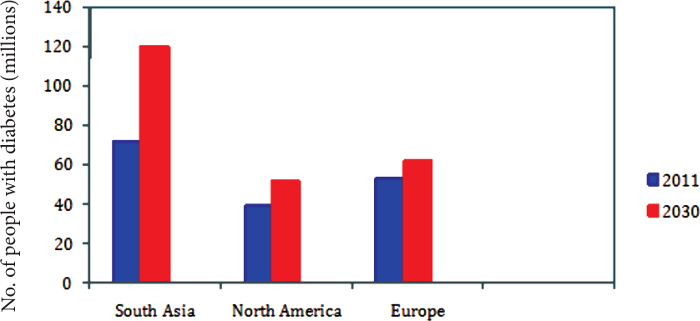
\includegraphics{images/033.jpg}
\caption{\textbf{ಶವಾಸನ} }
\end{figure}

\textbf{ \general{\enginline{11.}} ಶವಾಸನ:} ಈ ಆಸನವನ್ನು ನಡೆಸುವ ಮುಖ್ಯ ಉದ್ದೇಶ ದೇಹ ಮತ್ತು ಮನಸ್ಸನ್ನು ಸ್ತಬ್ದ ಹಾಗೂ ಶಾಂತವಾಗಿಟ್ಟುಕೊಂಡು ಅವಕ್ಕೆ ಸಂಪೂರ್ಣ ವಿಶ್ರಾಂತಿಯನ್ನೊದಗಿಸುವುದಾಗಿದೆ. ಇದು ಮೇಲ್ನೋಟಕ್ಕೆ ಸುಲಭವಾಗಿ ತೋರಿದರೂ ಇದರ ವಿಧಾನ, ಸರಿಯಾದ ಆಚರಣೆ, ತಿಳಿದುಕೊಳ್ಳುವುದು ಕಷ್ಟಕರವಾಗಿಯೇ ಇದೆ. ಒಂದು ಯೋಗಾಸನ ಮುಗಿಸಿ, ಇನ್ನೊಂದನ್ನಾರಂಭಿಸುವ ಮೊದಲು ಈ ಶವಾಸನ ಮಾಡಿದರೆ ಒಳ್ಳೆಯದು. ಅದರಿಂದ ದೇಹ ಮನಸ್ಸುಗಳಿಗೆ ಆಯಾಸವಾಗುವುದು ತೋರಿಬರುವುದಿಲ್ಲ. ಮಾತ್ರವಲ್ಲದೆ, ಒಂದು ತರದ ಶಾಂತಿ ಸಮಾಧಾನವೂ ಒದಗುತ್ತದೆ.

ಈ ಆಸನದಲ್ಲಿ ಮೊತ್ತಮೊದಲು ನಾವು ನೆಲದ ಮೇಲೆ ಅಂಗಾತ ಮಲಗಿಕೊಂಡು ಸಂಪೂರ್ಣ ವಿಶ್ರಾಂತಿಯನ್ನು ಅನುಭವಿಸಲಾರಂಭಿಸಬೇಕು. ನಿಧಾನವಾಗಿ ಕಾಲಬೆರಳಿಂದಾರಂಭಿಸಿ ತಲೆಕೂದಲವರೆಗೆ ಒಂದೊಂದೇ ಅವಯವಗಳಲ್ಲಿ ಸಂಪೂರ್ಣ ವಿಶ್ರಾಂತಿಯನ್ನು ಭಾವಿಸುತ್ತ ಬರಬೇಕು. ಕೆಳಗಿಂದ ಮೇಲಿನವರೆಗಿನ ಒಂದೊಂದೇ ಅಂಗಗಳನ್ನು 'ಶವ'ದಂತೆ ಸ್ತಬ್ಧ–ನಿಶ್ಚೇಷ್ಟ, ನಿರ್ಜಿವ ಎಂದು ಭಾವಿಸಿಕೊಂಡು ಬರಬೇಕು. ದೇಹ, ಮನಸ್ಸು, ಬುದ್ಧಿಗಳಿಗೆ ಪರಿಪೂರ್ಣ ಶಾಂತಿಯನ್ನು ಭಾವಿಸಬೇಕು. ಬೇರಾವ ವಿಚಾರದತ್ತವೂ ಮನಸ್ಸನ್ನು ಹರಿಯಬಿಡ. ಬಾರದು.

ಈ ಸ್ಥಿತಿಯಲ್ಲಿ ಐದರಿಂದ ಹದಿನೈದು ನಿಮಿಷಗಳವರೆಗೆ ಶಾಂತಚಿತ್ತರಾಗಿ ಮಲಗಿಕೊಂಡಿರಬೇಕು.

ಹೀಗೆ ಮಾಡುವುದರಿಂದ ದೇಹ ಮನಸ್ಸುಗಳೆರಡಕ್ಕೂ ಎಲ್ಲ ತರದ ಆರಾಮ ದೊರಕುತ್ತದೆ. ನಂತರ ಎಂತಹ ಕೆಲಸ ನಡೆಸುವುದಕ್ಕೂ ಹೊಸ ಹುರುಪು ಒದಗಿ ಬರುತ್ತದೆ. ಇತ್ತೀಚೆ, ಈ ವಿಚಾರದಲ್ಲಿ ತುಂಬ ಸಂಶೋಧನೆಗಳು ನಡೆದಿವೆ. ಹೆಚ್ಚಿದ ರಕ್ತದ ಒತ್ತಡ, ಎದೆ ಸೆಳೆವು ಮುಂತಾದ ಬೇರೆ ಬೇರೆ ತರದ ಹೃದಯ ರೋಗಗಳಿಗೆ ಇದು ಉತ್ತಮ ಶಾಮಕ ಉಪಚಾರವೆಂದು ಕಂಡುಕೊಂಡಿದ್ದಾರೆ. ಹೆಚ್ಚಿನ ಶ್ರಮವನ್ನುಂಟುಮಾಡುವ ಇತರ ಯೋಗಾಭ್ಯಾಸಗಳು ಇಂಥವರಿಗೆ ಸರಿ ಹೋಗುವುದಿಲ್ಲ. ಆದ್ದರಿಂದ ಇವರಿಗೆ ಸರಿಯಾದ ರೀತಿಯ ಶವಾಸನ ಸುಲಭವೂ ಪರಿಣಾಮಕಾರಿ ಔಷಧಿಯೂ ಆಗಿದೆ.

\textbf{ \general{\enginline{12.}} ಸೂರ್ಯ ನಮಸ್ಕಾರ:} ಕ್ರಮವಾದ ಯೋಗಾಭ್ಯಾಸಗಳಲ್ಲೊಂದಾಗಿ ಸೂರ್ಯ ನಮಸ್ಕಾರವನ್ನು ಹೇಳಲಾಗಿಲ್ಲ. ಹಾಗಿದ್ದರೂ ಸಹ, ಹಲವು ಯೋಗಾಭ್ಯಾಸಗಳ ಮೂಲತತ್ವಗಳನ್ನೊಳಗೊಂಡಿರುವ ಕಾರಣ ಇದನ್ನು ಸಕಲ ಯೋಗಸಾರವೆಂದು ಹೇಳಲಾಗಿದೆ. ಮಾತ್ರವಲ್ಲದೆ ಅಪಾರ ತೇಜಸ್ಸಿನ ಮೂಲಧಾರನಾದ ಸೂರ್ಯನ ವಂದನೆಯೂ ಸೇರಿರುವ ಕಾರಣ ಇದು ಆಧ್ಯಾತ್ಮಿಕತೆಯನ್ನೂ ಒಳಗೊಂಡಿದೆ. ಸ್ವಾಮಿ ಸತ್ಯಾನಂದರು ಈ ವಿಚಾರದಲ್ಲಿ ಹೀಗೆ ಹೇಳುತ್ತಾರೆ.'ಸೂರ್ಯ ನಮಸ್ಕಾರವು ಬಹಳ ಶಕ್ತಿಯುತವಾದ ವ್ಯಾಯಾಮವಾಗಿದೆ. ಇದೊಂದು ಆಸನವಲ್ಲ. ಅಥವಾ ಸಾಂಪ್ರದಾಯಿಕ ಯೋಗದ ಒಂದು ಭಾಗವೂ ಅಲ್ಲ. ಆದರೆ ಈ ಸೂರ್ಯನಮಸ್ಕಾರವನ್ನು ಯೋಗಾಭ್ಯಾಸದ ಪ್ರಮುಖ ಅಂಗವಾಗಿ ನಿತ್ಯ ನಡೆಸಿಕೊಂಡು ಬರುವುದು ಬಹಳ ಒಳ್ಳೇದು. ಇದು ಇಡೀ ದೇಹವನ್ನೇ ಪುನರುಜ್ಜೀವನಗೊಳಿಸುತ್ತದೆ. ಎಲ್ಲ ತರದ ಆಲಸ್ಯವನ್ನು ಹೋಗಲಾಡಿಸುತ್ತದೆ. ಮಾತ್ರವಲ್ಲದೆ ಮುಂದೆ ನಡೆಸಲಿರುವ ಆಸನ, ಪ್ರಾಣಾಯಾಮ, ಧ್ಯಾನ– ಮುಂತಾದವುಗಳಿಗೆ ನಮ್ಮ ದೇಹ ಮನಸ್ಸುಗಳನ್ನು ಸಂಪೂರ್ಣ ಸಿದ್ಧಗೊಳಿಸುತ್ತದೆ. ಇವುಗಳಿಂದ ಅತಿ ಹೆಚ್ಚಿನ ಪ್ರಯೋಜನ ಸಿಗುವಂತೆಯೂ ಆಗುತ್ತದೆ.

\begin{figure}
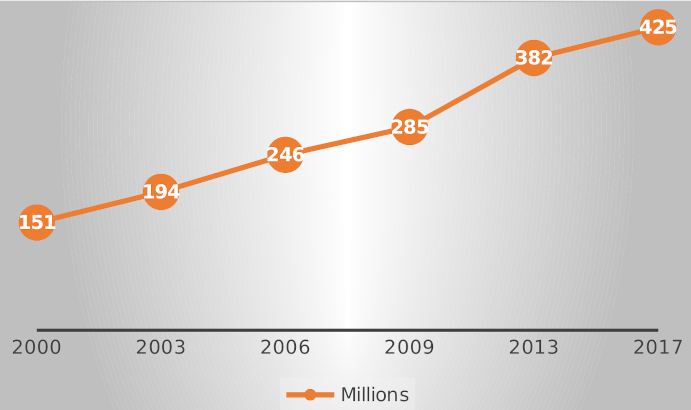
\includegraphics{images/034.jpg}
\end{figure}

\textbf{ವಿಧಾನ:} ಇದರಲ್ಲಿ ಹನ್ನೆರಡು ತರದ ದೈಹಿಕ ಅಂಗವಿನ್ಯಾಸಗಳಿವೆ. ಅವನ್ನು ಕ್ರಮವಾಗಿ ಒಂದರ ನಂತರ ಒಂದರಂತೆ ನಡೆಸಿಕೊಂಡು ಹೋಗಬೇಕು. ಅದರೊಂದಿಗೆ ಶ್ವಾಸೋಚ್ಛ್ವಾಸ ವಿಧಾನ ಮತ್ತು ಸೂರ್ಯದೇವನ ವಂದನೆಗಳನ್ನು ಸೇರಿಸಿಕೊಂಡರೆ, ಈ ಸೂರ್ಯನಮಸ್ಕಾರದಿಂದ ಇನ್ನೂ ಹೆಚ್ಚಿನ ಉಪಯೋಗ ದೊರಕುತ್ತದೆ.

ಅಂಗವಿನ್ಯಾಸ– \enginline{1.} ಇದು ಪ್ರಾರ್ಥನಾ ಭಂಗಿ. ನೆಟ್ಟಗೆ ನಿಂತುಕೊಂಡು ಎರಡೂ ಪಾದಗಳನ್ನು ಜೋಡಿಸಿಕೊಳ್ಳಬೇಕು. ಮುಂದಕ್ಕೆ ತಂದ ಎದೆಯ ಮೇಲೆ ಕೈಜೋಡಿಸಿ ನಮಸ್ಕರಿಸುತ್ತ ಸೂರ್ಯದೇವನ ಧ್ಯಾನಗೈಯ್ಯಬೇಕು.

\enginline{2.} ನಂತರ ಎರಡು ಭುಜಗಳನ್ನು ತಲೆಯ ಮೇಲೆತ್ತಿಕೊಂಡು ಬಾಹು, ಬೆನ್ನು ತಲೆಗಳನ್ನು ಆದಷ್ಟು ಹಿಂದಕ್ಕೆ ಬಾಗಿಸಬೇಕು. ಆಗ ಶ್ವಾಸವನ್ನು ನಿಧಾನವಾಗಿ ಮತ್ತು ಆಳವಾಗಿ ಒಳಕ್ಕೆಳೆದುಕೊಳ್ಳಬೇಕು.

\enginline{3.} ಆಮೇಲೆ ಮುಂದಕ್ಕೆ ಬಾಗಿ ಎರಡೂ ಅಂಗೈಗಳನ್ನು ನೆಲದ ಮೇಲಿಡಬೇಕು. ಆಗ ಮೊಣಕಾಲುಗಳನ್ನು ಬಗ್ಗಿಸಬಾರದು, ಮೂಗನ್ನು ಮೊಣಗಂಟಿಗೆ ತಾಗಿಸಿ ನಿಧಾನವಾಗಿ ಶ್ವಾಸ ಹೊರಬಿಡಬೇಕು.

\enginline{4.} ಆ ನಂತರ ಎಡಗಾಲನ್ನು ಸಾಧ್ಯವಾದಷ್ಟು ಹಿಂದಕ್ಕೆ ಚಾಚಬೇಕು. ಬಲಗಾಲನ್ನು ಮೊಣಗಂಟಿನಲ್ಲಿ ಬಾಗಿಸಿಟ್ಟುಕೊಳ್ಳಬೇಕು. ಕೈಗಳು ನೆಲದ ಮೇಲೆಯೇ ನೆಟ್ಟಗಿರಬೇಕು. ತಲೆ, ಬೆನ್ನು, ಕುತ್ತಿಗೆಗಳನ್ನು ಸಾಧ್ಯವಿದ್ದಷ್ಟು ಹಿಂದಕ್ಕೆ ಬಾಗಿಸಬೇಕು. ಆಗ ಶ್ವಾಸವನ್ನು ಪುನಃ ಆಳವಾಗಿ ಒಳಕ್ಕೆಳೆದುಕೊಳ್ಳಬೇಕು.

\enginline{5.} ಈಗ ಎಡಗಾಲನ್ನು ಹಿಂದಕ್ಕೆ ಚಾಚಿ ಬಲಗಾಲಿನೊಂದಿಗೆ ಜೋಡಿಸಿಟ್ಟು ಕೊಳ್ಳಬೇಕು. ಸೊಂಟವನ್ನು ಆದಷ್ಟು ಮೇಲಕ್ಕೆತ್ತಿ ತಲೆಯನ್ನು ಕೆಳಕ್ಕೆ ಬಾಗಿಸಿ ಬಾಹುಗಳ ಮಧ್ಯದಲ್ಲಿಟ್ಟುಕೊಳ್ಳಬೇಕು. ಈಗ ಶ್ವಾಸವನ್ನು ಧರಿಸಿಕೊಂಡೇ ಇರಬೇಕು.

\enginline{6.} ನಂತರ ಬಾಹುಗಳನ್ನು ಬಗ್ಗಿಸಿ ತಲೆ ಮತ್ತು ಎದೆಯನ್ನು ನೆಲದತ್ತ ತರಬೇಕು. ಆದರೆ ಹೊಟ್ಟೆ ಮತ್ತು ಸೊಂಟ, ನೆಲದಿಂದ ಮೇಲಕ್ಕೇ ಇರಬೇಕು. ಕಾಲಗಂಟು ನೆಲಕ್ಕೆ ತಾಗಿರಬೇಕು. ಈಗ ಧಾರಣೆ ಮಾಡಿಕೊಂಡಿದ್ದ ಶ್ವಾಸವನ್ನು ಬಿಡಬೇಕು.

\enginline{7.} ಈಗ ಸೊಂಟವನ್ನು ನೆಲಕ್ಕೆ ಮುಟ್ಟಿಸಿ ಎದೆ, ಕುತ್ತಿಗೆ ಮತ್ತು ತಲೆಯನ್ನು ಎತ್ತಿ ಹಿಂದಕ್ಕೆ ಬಾಗಿಸಬೇಕು. ಆಗ ಭುಜಗಳನ್ನು ನೆಟ್ಟಗಾಗಿಸಿ ಹಿಂದೆ ಹೇಳಿದ್ದ ಭುಜಂಗಾಸನದ ಸ್ಥಿತಿಗೆ ಬರಬೇಕು. ಈಗ ಪುನಃ ಆಳವಾಗಿ ಶ್ವಾಸವನ್ನೊಳಕ್ಕೆಳೆದುಕೊಳ್ಳಬೇಕು.

\enginline{8.} ಈಗ ಐದನೆಯ ಹಂತದ ಅಂಗವಿನ್ಯಾಸವನ್ನು ಪುನರಾವರ್ತಿಸಬೇಕು ಮತ್ತು ಶ್ವಾಸವನ್ನು ಹೊರಬಿಡಬೇಕು.

\enginline{9.} ಈಗ ನಾಲ್ಕನೆಯ ಅಂಗವಿನ್ಯಾಸವನ್ನು ಪುನರಾವೃತ್ತಿ ಮಾಡಬೇಕು. ಆದರೆ ಈಗ ಎಡಗಾಲ ಬದಲಾಗಿ ಬಲಗಾಲನ್ನು ಬಾಗಿಸಬೇಕು. ಎಡಗಾಲು ನೆಟ್ಟಗಾಗಿರಬೇಕು. ಪುನಃ ಆಳವಾಗಿ ಶ್ವಾಸವನ್ನೆಳೆದುಕೊಳ್ಳಬೇಕು..

\enginline{10.} ಇದೀಗ ಮೂರನೆಯ ಹಂತದ ಅಂಗವಿನ್ಯಾಸದ ಪುನರಾವೃತ್ತಿಯಾಗಿದೆ. ಅಂದರೆ ತಲೆಯನ್ನು ಕೆಳಕ್ಕೆ ಬಾಗಿಸಿ ಶ್ವಾಸ ಹೊರಬಿಡಬೇಕು.

\enginline{11.} ಇದು ಎರಡನೆಯ ಹಂತದಲ್ಲಿ ಹೇಳಿದಂತೆ ತಲೆ, ಎದೆ, ಬಾಹುಗಳನ್ನು ಹಿಂದಕ್ಕೆ ಬಾಗಿಸಿ ದೀರ್ಘಶ್ವಾಸವನ್ನು ಒಳಕ್ಕೆಳೆದುಕೊಳ್ಳಬೇಕು.

\enginline{12.} ಇದು ಒಂದನೆಯ ಅಂಗವಿನ್ಯಾಸದಲ್ಲಿ ಹೇಳಿದ ಅಂತಿಮ ಹಂತವಾಗಿದೆ. ಈಗ ಸಂಪೂರ್ಣ ಶ್ವಾಸ ಹೊರಬಿಟ್ಟು ಒಮ್ಮೆಗೆ ಪರಿಪೂರ್ಣ ವಿಶ್ರಾಂತಿ ಹೊಂದಿಕೊಳ್ಳಬೇಕು.

ಹೀಗೆ \enginline{12} ತರದ ಅಂಗವಿನ್ಯಾಸವುಳ್ಳ ಒಂದು ಆವೃತ್ತಿಗೆ ಒಂದು ಸೂರ್ಯ ನಮಸ್ಕಾರವೆಂದು ಹೇಳುತ್ತಾರೆ. ಮೇಲೆ ಹೇಳಿದ ವಿವರಣೆಯನ್ನು ಚಿತ್ರ ನೋಡಿ ಮಂದಟ್ಟು ಮಾಡಿಕೊಳ್ಳಬೇಕು.

ಸಾಧಾರಣವಾಗಿ ಇಂತಹ ಸೂರ್ಯ ನಮಸ್ಕಾರವನ್ನು ಹತ್ತು ಸಲ ನಡೆಸಬೇಕು.ಆದರೆ ಇದು ವೈಯಕ್ತಿಕ ದೇಹಶಕ್ತಿಯನ್ನವಲಂಬಿಸಿದೆ. ಈ ಸೂರ್ಯ ನಮಸ್ಕಾರವನ್ನು ಹೆಚ್ಚಿನ ದೇಹಾಯಾಸವನ್ನುಂಟುಮಾಡಿಕೊಳ್ಳದೆ ಸುಖವಾಗಿ ನಡೆಸಿಕೊಂಡು ಹೋಗಬೇಕಲ್ಲದೆ, ಗುರಿ ಮುಟ್ಟುವುದಕ್ಕೋಸ್ಕರ ಮಿತಿಮೀರಿದ ದೇಹಶ್ರಮ ಮಾಡಿಕೊಳ್ಳಬಾರದು. ಒಂದು ತರದ ತಾಳಕ್ಕನುಗುಣವಾಗಿ, ಮೇಲೆ ಹೇಳಿದಂತೆ ಶ್ವಾಸೋಚ್ಛ್ವಾಸಗಳನ್ನು ನಿಯಂತ್ರಿಸಿಕೊಂಡು ಇದನ್ನು ಕ್ರಮವಾಗಿ ನಡೆಸಿಕೊಂಡು ಬರಬೇಕು. ಇದಕ್ಕೆ ಬೇಕಾಗುವ ಸಮಯವನ್ನು ಸಹ, ಅವರವರ ಶಕ್ತಿಗನುಗುಣವಾಗಿ ಅಳವಡಿಸಿಕೊಳ್ಳಬೇಕು. ಸಾಧಾರಣವಾಗಿ ಹತ್ತು ಸೂರ್ಯನಮಸ್ಕಾರಗಳನ್ನು ಐದು ನಿಮಿಷಗಳಲ್ಲಿ ಮಾಡಿ ಮುಗಿಸುತ್ತಾರೆ. ಆದರೆ ಬೇಕಾಗುವ ಸಮಯ ಮತ್ತು ಸೂರ್ಯನಮಸ್ಕಾರಗಳ ಸಂಖ್ಯೆಯನ್ನು ವ್ಯಕ್ತಿಯ ಶಕ್ತಿಗನುಗುಣವಾಗಿಟ್ಟುಕೊಳ್ಳುವುದುತ್ತಮ.

ಇದನ್ನು ನಡೆಸುವುದಕ್ಕೆ ಅತ್ಯಂತ ಯೋಗ್ಯ ಸಮಯವೆಂದರೆ ಪ್ರಾತಃಕಾಲ. ಉದಯಿಸುತ್ತಿರುವ ಸೂರ್ಯದೇವನಿಗಿದಿರಾಗಿ ನಮಸ್ಕಾರಗೈದರೆ ಪುಣ್ಯ ಪುರುಷಾರ್ಥಗಳೆರಡೂ ಒದಗಿದಂತಾಗುತ್ತದೆ. ಆದರೆ ಕೆಲಸಂದರ್ಭದಲ್ಲಿ ಇದು ಆಗದಿರಲೂಬಹುದು. ಆಗ ಒಳ್ಳೆಯ ಗಾಳಿ ಬೆಳಕು ಬರುವ ಕೋಣೆಯಲ್ಲಿ ಮುಂಜಾನೆ ಬರಿಹೊಟ್ಟೆಯಲ್ಲಿ ಈ ನಮಸ್ಕಾರ ಕಾರ್ಯ ನಡೆಸಬೇಕು. ಇದು ಮುಂದೆ ನಡೆಸಲಿರುವ ಇತರ ಯೋಗಾಭ್ಯಾಸಗಳ ಪೂರ್ವಭಾವಿ ಕ್ರಿಯೆಯೂ ಆಗುತ್ತದೆ. ಅತಿ ಕಡಿಮೆ ವಸ್ತ್ರ ಧರಿಸಿಕೊಂಡು, ಬಾಗುವಾಗ ಅಥವಾ ಏಳುವಾಗ ಬಿಗಿವಸ್ತ್ರದ ಹಿಡಿತದಿಂದ ತೊಂದರೆಯಾಗದಂತೆ ನೋಡಿಕೊಳ್ಳಬೇಕು. ಇದನ್ನು ಪುರುಷರೂ ಸ್ತ್ರೀಯರೂ ವಯೋಮಾನದ ಭೇದವಿಲ್ಲದೆ ನಡೆಸಿಕೊಂಡು ಬರಬಹುದು. ಆದರೆ ಮಹಿಳೆ ಗರ್ಭಿಣಿಯಾಗಿರುವಾಗ ಅಥವಾ ಬಹಿಷ್ಠೆಯಾಗಿರುವಾಗ ನಡೆಸಬಾರದು. ಈ ವಿಚಾರದಲ್ಲಿ ಸ್ವಾಮಿ ಸತ್ಯಾನಂದರು ತಮ್ಮ ಕ್ರಿಯಾ ಯೋಗದಲ್ಲಿ ಹೀಗೆ ಹೇಳಿದ್ದಾರೆ– `ಇಂದಿನ ನಗರ ಜೀವನದ ಜಂಝಾಟಕ್ಕೊಳಗಾಗಿದ್ದು ಸಾಕಷ್ಟು ವ್ಯಾಯಾಮಗೈಯಲು ಸಮಯ, ಜಾಗವಿಲ್ಲದ ಜನರಿಗೆ ಸೂರ್ಯ ನಮಸ್ಕಾರವು ಒಂದು ದೊಡ್ಡ ವರಪ್ರದಾನವಾಗಿದೆ.'

ಪ್ರಸ್ತುತ, ನಗರನಿವಾಸಿಗಳೇ ಹೆಚ್ಚಿನ ಒತ್ತಡದ ಕಾವುನೋವುಗಳಿಂದ ತೊಳಲಾ ಡುತ್ತಿರುವವರು. ದೇಹಕ್ಕೆ ವ್ಯಾಯಮವಿಲ್ಲದ, ಮನಸ್ಸಿಗೆ ಶಾಂತಿ ಇಲ್ಲದ, ಜೀವನ ವಿಧಾನವೇ ಅದಕ್ಕೆ ಪ್ರಧಾನ ಕಾರಣ. ಸರಿಯಾದ ಸೂರ್ಯ ನಮಸ್ಕಾರವೇ ಇದಕ್ಕೆ ತಕ್ಕ ಪರಿಹಾರಮಾರ್ಗ. ಇದನ್ನು ಯೋಗಾಭ್ಯಾಸದೊಂದಿಗೆ ನಡೆಸಿದರೆ ಇನ್ನೂ ಉತ್ತಮ. ಅದು ಸಾಧ್ಯವಿಲ್ಲವಾದರೆ ಬರೇ ಸೂರ್ಯ ನಮಸ್ಕಾರವನ್ನಾದರೂ ನಿತ್ಯ ಮಾಡುತ್ತ ಬಂದರೆ ಎಷ್ಟೋ ಸಮಸ್ಯೆಗಳು ಪರಿಹಾರವಾಗಬಲ್ಲವು. ಸುಖ ಜೀವನ ಸಾಗಿಸಲು ಸಾಧ್ಯವೂ ಆಗಬಹುದು.

\textbf{ಪ್ರಾಣಾಯಾಮ:} ಪ್ರಾಣ ಅಂದರೆ ಉಸಿರು. ಉಸಿರಾಟದ ವ್ಯಾಯಾಮಕ್ಕೆ ಪ್ರಾಣಾಯಾಮವೆಂದು ಹೆಸರು. ನಿಧಾನವಾಗಿ ಉಸಿರನ್ನು ಒಳಕ್ಕೆ ಎಳೆದುಕೊಂಡು, ಆದಷ್ಟು ಹೆಚ್ಚು ಸಮಯ ಅದನ್ನು ಒಳಗೆ ಕಟ್ಟಿಕೊಂಡು, ಆಮೇಲೆ ನಿಧಾನವಾಗಿ ಹೊರಬಿಡುವುದೇ ಪ್ರಾಣಾಯಾಮವಾಗಿದೆ. ಪ್ರತಿದಿನ ಇಂತಹ ಪ್ರಾಣಾಯಾಮ ಮಾಡುವುದರಿಂದ ಹೃದಯ, ಶ್ವಾಸೋಚ್ಛ್ವಾಸಗಳ ಪ್ರಕ್ರಿಯೆ ಸುಧಾರಣೆಗೊಳ್ಳುತ್ತದೆ. ಮಾತ್ರವಲ್ಲದೆ ಕಾಲಕ್ರಮೇಣ ಹೊಸ ಉಸಿರಾಟದ ಕ್ರಮವನ್ನೇ ಅರಿತು ಕೊಳ್ಳುವುದಕ್ಕೆ ಸಾಧ್ಯವಾಗುತ್ತದೆ. ಇದಲ್ಲದೆ ಮಿದುಳಿನ ಅತಿಸೂಕ್ಷ್ಮ ನರಕೋಶಗಳಿಗೆ ಹೆಚ್ಚಿನ ಆಮ್ಲಜನಕ ದೊರಕಿ ಮನಃಶಾಂತಿಯು ಒದಗಿಬರುತ್ತದೆ. ಅಂತಹ ಮನಃಶಾಂತಿಯಿಂದಾಗಿ ಕ್ರಮೇಣ ಏಕಾಗ್ರತೆ ಹಾಗೂ ಧ್ಯಾನ ನಡೆಸಲು ಸಾಧ್ಯವಾಗುತ್ತದೆ. ಯೋಗಾಭ್ಯಾಸದ ಅಂತಿಮ ಗುರಿಯಾದ ಸಮಾಧಿ ಸಾಧನೆಗೂ ಇದು ಸಹಾಯಕವಾಗುತ್ತದೆ.

\begin{center}
\enginline{\textbf{Techinique of Pranayama}}
\end{center}


\begin{figure}
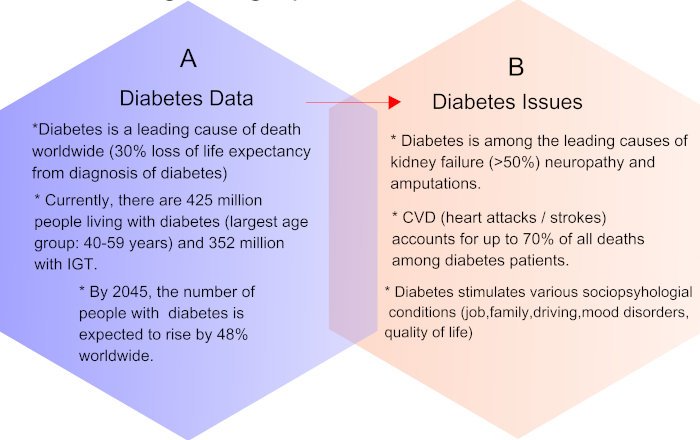
\includegraphics{images/035.jpg}
\caption{\textbf{ಪ್ರಾಣಾಯಾಮ ನಿಧಾನ} }
\end{figure}

ಪ್ರಾಣಾಯಾಮವನ್ನು ಯೋಗಾಭ್ಯಾಸದ ನಂತರ, ಧ್ಯಾನವನ್ನು ಆರಂಭಿಸುವ ಮೊದಲು ನಡೆಸಬೇಕು. ಇದರಲ್ಲಿ ಮೂರು ಹಂತಗಳಿರುತ್ತವೆ. ಮೊದಲು ಪೂರಕ ಅಂದರೆ ಶ್ವಾಸವನ್ನೊಳಕ್ಕೆ ತೆಗೆದುಕೊಳ್ಳುವುದು. ನಂತರ ಕುಂಭಕ ಅಂದರೆ ಉಸಿರನ್ನು ಬರಕ್ಕೆ ತಡೆಹಿಡಿದುಕೊಳ್ಳುವುದು ಮತ್ತು ಕೊನೆಯದಾದ ರೇಚಕ ಅಂದರೆ ಉಸಿರನ್ನು ಹೊರಬಿಡುವುದು. ಕೆಲವು ತಜ್ಞರ ಪ್ರಕಾರ ಈ ಪ್ರತಿ ಒಂದು ಹಂತದಲ್ಲಿಯೂ ಒಂದು ತರದ ಸಮಯದ ನಿಯತಿ ಇರಬೇಕು. ಪೂರಕಕ್ಕೆ ಎರಡು ಸೆಕೆಂಡುಗಳು ಬೇಕಾದರೆ ಕುಂಭಕಕ್ಕೆ ಎಂಟು ಸೆಕೆಂಡುಗಳು, ನಂತರ ರೇಚಕಕ್ಕೆ ನಾಲ್ಕು ಸೆಕೆಂಡುಗಳು. ಹೀಗೆ \enginline{1: 4: 2} ರ ಪ್ರಮಾಣದಲ್ಲಿ ಇರಬೇಕು.

ಇಂತಹ ಕ್ರಮಬದ್ಧವಾದ ಕಾಲನಿಯಮಿತ ಪ್ರಾಣಾಯಾಮದ ಅಭ್ಯಾಸವು ಕಷ್ಟಕರವಾದ ಮನಸ್ಸಿನ ಏಕಾಗ್ರತೆಯ ಸಾಧನೆ ಹಾಗೂ ಧ್ಯಾನ ಸಾಧನೆಗೆ ತುಂಬಾ ಸಹಾಯಕವಾಗುತ್ತದೆ. ಆದರೆ ಸರಿಯಾದ ರೀತಿಯಲ್ಲಿ ಈ ಪ್ರಾಣಾಯಾಮ ಮಾಡದಿದ್ದರೆ ಅದರಿಂದ ಪ್ರತಿಕೂಲ ಪರಿಣಾಮ ಉಂಟಾಗಲೂಬಹುದು. ವಾಸ್ತವಿಕವಾಗಿ ಇದನ್ನು ಬಹಳ ಎಚ್ಚರಿಕೆಯಿಂದ, ನಿಧಾನವಾಗಿ ಯಾವುದೇ ತರದ ಭಾವೋದ್ವೇಗಗಳಿಲ್ಲದೆ, ಶಾಂತಚಿತ್ತದಿಂದ ಆರಂಭಿಸಬೇಕು. ಈ ತರದ ಮುಂಜಾಗ್ರತೆ ತೆಗೆದುಕೊಳ್ಳದಿದ್ದರೆ ಕಟ್ಟುಸಿರು, ಕೆಮ್ಮು, ತಲೆನೋವು ಮುಂತಾದ ಹೂಸ ಖಾಯಿಲೆಗಳು ತಲೆದೋರಲೂಬಹುದು. ಆದ್ದರಿಂದ ಈ ವಿಚಾರವನ್ನರಿತ ಸಮರ್ಥಗುರುವಿನ ಬಳಿ ಉಪದೇಶ ಪಡೆದುಕೊಂಡು ಈ ಪ್ರಾಣಾಯಾಮವನ್ನು ಆರಂಭಿಸುವುದೊಳ್ಳೇದು. ಪ್ರತಿನಿತ್ಯ ಸರಿಯಾದ ರೀತಿಯಲ್ಲಿ ಇದನ್ನು ಮಾಡಿಕೊಂಡು ಬಂದರೆ ಜೀವನದ ಎಂತಹ ಸಮಸ್ಯೆಗಳನ್ನೆದುರಿಸಲೂ ಬೇಕಾದ ಶಕ್ತಿ, ಉತ್ಸಾಹ ಒದಗಿ ಬರುತ್ತದೆ.

\textbf{ವಿಧಾನ:} ಸಾಮಾನ್ಯವಾಗಿ ಬೆಳಗ್ಗೆದ್ದು ಮಲಮೂತ್ರ ವಿಸರ್ಜನೆಗೈದ ಬಳಿಕ ಪ್ರಾಣಾಯಮವನ್ನಾರಂಭಿಸಬೇಕು. ಇದಕ್ಕಿರುವ ನೆಲದ ಮೇಲೆ ಒಂದು ಜಾಗ ಒಳ್ಳೆಯ ಗಾಳಿ ಬೆಳಕುಗಳಿಂದ ಕೂಡಿರಬೇಕು. ನೆಲದ ಮೇಲೆ ಒಂದು ಹುಲ್ಲು ಚಾಪೆ ಅಥವಾ ಸಣ್ಣ ತೆಳುಹಾಸು ಹಾಕಿ ಅದರ ಮೇಲೆ ಪದ್ಮಾಸನದಲ್ಲಿ ಸುಖವಾಗಿ ಕುಳಿತುಕೊಳ್ಳಬೇಕು. ಹಾಗೆ ಕುಳಿತುಕೊಂಡಾಗ ದೇಹದ ಯಾವ ಭಾಗಕ್ಕೂ ನೋವು ತಡೆಗಳಿರಬಾರದು. ಕುತ್ತಿಗೆ ನೆಟ್ಟಗಿರಬೇಕು. ಕಣ್ಣು ಮುಚ್ಚಿಕೊಂಡು ಇಷ್ಟದೇವರ ಧ್ಯಾನ ಮಾಡಿಕೊಂಡಿದ್ದರೆ ಒಳ್ಳೇದು. ಬಲ ನಾಸಾರಂಧ್ರವನ್ನು ಹೆಬ್ಬೆರಳಿನಿಂದಲೂ, ಎಡ ನಾಸಾರಂಧ್ರವನ್ನು ನಡುಬೆರಳಿಂದಲೂ ಬೇಕಾದಾಗ ಒತ್ತಿಕೊಂಡು ಶ್ವಾಸ ನಿಯಂತ್ರಣ ಮಾಡಿಕೊಳ್ಳುತ್ತಿರಬೇಕು. ತೋರ್ಬೆರಳನ್ನು ಮೂಗಿನ ಮೇಲೆ ಇಟ್ಟುಕೊಂಡಿರಬೇಕು.

ಮೊತ್ತಮೊದಲು ಎಡ ನಾಸಾರಂಧ್ರದಿಂದ ದೀರ್ಘಶ್ವಾಸವನ್ನು ನಿಧಾನವಾಗಿ ಸಾಮಾನ್ಯ ಎರಡು ಸೆಕೆಂಡುಗಳಷ್ಟು ಕಾಲ ಮೇಲಕ್ಕೆಳೆದುಕೊಳ್ಳಬೇಕು. ಆಗ ಹೆಬ್ಬೆರಳಿಂದ ಬಲನಾಸಾರಂಧ್ರವನ್ನು ಒತ್ತಿಹಿಡಿದುಕೊಳ್ಳಬೇಕು. ಧ್ವನಿ ತಂತುಗಳನ್ನು ಮುಚ್ಚಿ ಕೊಳ್ಳುವ ಮೂಲಕ, ಶ್ವಾಸವು ನಿಯತವಾದ ಒತ್ತಡದೊಂದಿಗೆ ಶ್ವಾಸಕೋಶವನ್ನು ನಿಧಾನವಾಗಿ ಪ್ರವೇಶಿಸುವಂತಾಗಬೇಕು. ಹಾಗೆ ತುಂಬಿದ ಶ್ವಾಸವನ್ನು ಸಾಮಾನ್ಯ ಎಂಟು ಸೆಕೆಂಡುಗಳವರೆಗೆ ತಡೆದಿಟ್ಟುಕೊಂಡಿರಬೇಕು. ನಂತರ ನಿಧಾನವಾಗಿ ಬಲ ನಾಸಾರಂಧ್ರದಿಂದ ಹೊರಬಿಡಬೇಕು. ಆಗ ಎಡ ನಾಸಾರಂಧ್ರವನ್ನು ಬೆರಳಿನಿಂದ ಮುಚ್ಚಿಕೊಂಡಿರಬೇಕು. ಹಾಗೆ ಶ್ವಾಸ ಹೊರಬರಲು ಸಾಮಾನ್ಯ ನಾಲ್ಕು ಸೆಕೆಂಡು ಸಮಯ ಬಳಸಬೇಕು. ಆಮೇಲೆ ಒಂದು ಸಾದಾ ಶ್ವಾಸೋಚ್ಛ್ವಾಸದ ವಿರಾಮ ಒದಗಿಸಬೇಕು. ನಂತರ ಹಿಂದೆ ಹೇಳಿದ ರೀತಿಯಲ್ಲೇ ಎರಡು ಸೆಕೆಂಡ್ ಬಲ ನಾಸಾರಂಧ್ರದಿಂದ ಶ್ವಾಸವನ್ನು ಒಳಕ್ಕೆಳೆದುಕೊಂಡು ಎಂಟು ಸೆಕೆಂಡು ಶ್ವಾಸವನ್ನು ತಡೆದಿಟ್ಟುಕೊಳ್ಳಬೇಕು. ಬಳಿಕ ನಿಧಾನವಾಗಿ ಎಡ ರಂಧ್ರದಿಂದ ನಾಲ್ಕು ಸೆಕೆಂಡುಗಳ ಕಾಲ ಹೊರಬಿಡಬೇಕು.

ಹೀಗೆ ದಿನಕ್ಕೆ \enginline{20} ಸಲ ಈ ತರದ ಪ್ರಾಣಾಯಾಮದ ಅಭ್ಯಾಸಗೈಯುತ್ತ ಬಂದರೆ ದೇಹ ಮನಸ್ಸುಗಳೆರಡರಲ್ಲೂ ಹೊಸ ಚೈತನ್ಯ ಶೀಘ್ರ ಮೂಡಿ ಬರುವಂತಾಗುತ್ತದೆ. ಮುಖದಲ್ಲಿ ಹೊಸ ಕಳೆ, ಹೊಸ ಹುರುಪು ಮೂಡಿ ಬರುತ್ತದೆ. ತನ್ನ ಪಾಲಿಗೆ ಬಂದ ಎಂತಹ ಕೆಲಸವನ್ನು ಸಹ ಧೈರ್ಯದಿಂದ ಮಾಡಿ ಮುಗಿಸಲು ಸಾಮರ್ಥ್ಯ ಒದಗಿಬರುತ್ತದೆ.

ಇದೀಗ ಪ್ರಮುಖವಾದ ಸರಳ ಪ್ರಾಣಾಯಾಮದ ವಿಧಾನವಾಗಿದೆ. ಆದರೆ ಇದಕ್ಕೂ ಮೀರಿದ ಹಲವಾರು ವಿಧಾನಗಳಿವೆ. ಅವನೆಲ್ಲ ಸಮರ್ಥ ಗುರುಗಳ ಸಹಾಯದಿಂದ ಕಲಿತುಕೊಳ್ಳಬೇಕು. ಬೇಕಿದ್ದರೆ ಅದಕ್ಕೆ ಸಂಬಂಧಪಟ್ಟ ಉದ್ಗ್ರಂಥಗಳಲ್ಲೂ ನೋಡಿಕೊಳ್ಳಬಹುದು.

\textbf{ಪ್ರತ್ಯಾಹಾರ ಅಥವಾ ಇಂದ್ರಿಯ ನಿಗ್ರಹ}

ದೇಹಕ್ಕೆ ಸಂಬಂಧಿಸಿದ ವ್ಯಾಯಾಮಗಳ ವಿಚಾರ ವಿವರಿಸಿಯಾದಮೇಲೆ ಈಗ ನಾವು ಮನಸ್ಸಿಗೆ ಸಂಬಂಧಿಸಿದ ವ್ಯಾಯಾಮ ವಿಚಾರ ತೆಗೆದುಕೊಳ್ಳುತ್ತಿದ್ದೇವೆ. ದೇಹದ ಮೇಲೆ ಮನಸ್ಸಿನ ಪ್ರಭಾವ ಧಾರಳವಾಗಿ ಒದಗಿಬರುತ್ತದೆ ಎಂಬುದು ಎಲ್ಲರೂ ತಿಳಿದಿರುವ ವಿಚಾರ. ಮನಸ್ಸು ಕದಡಿ ಹೋದಾಗ ದೇಹವೂ ಶಕ್ತಿಯನ್ನು ಕಳೆದುಕೊಳ್ಳುವುದಕ್ಕೆ ಆದಕಾರಣ ಮನಸ್ಸನ್ನು ಒಳ್ಳೆಯ ತರದಲ್ಲಿ ಹತೋಟಿಯಲ್ಲಿಟ್ಟುಕೊಳ್ಳುವುದಕ್ಕೆ ಪ್ರಯತ್ನಿಸಬೇಕು. ಆ ಮೂಲಕ ಮನಸ್ಸು ಕದಡದಂತೆ ಅಥವಾ ಕಳಂಕಿತವಾದರೂ ದೇಹದ ಮೇಲೆ ಅದರ ಹೆಚ್ಚಿನ ದುಷ್ಪರಿಣಾಮ ಬೀಳದಂಗೆ ನೋಡಿಕೊಳ್ಳಬೇಕು.

ಇದಕ್ಕಾಗಿ, ನಮ್ಮ ಕಣ್ಣು, ಕಿವಿ, ಮೂಗು, ನಾಲಗೆ, ಚರ್ಮ–ಎಂಬೀ ಪಂಚೇಂದ್ರಿಯಗಳ ಚಟುವಟಿಕೆಗಳ ಮೇಲೆ ಹಿಡಿತವನ್ನು ಸಾಧಿಸಬೇಕು. ಈ ಇಂದ್ರಿಯಗಳು ಮನಸ್ಸಿನ ಹಾಗೂ ದೇಹದ ಬಹಿರ್ದ್ವಾರಗಳಂತಿವೆ. ಈ ಇಂದ್ರಿಯಗಳನ್ನು ಉದ್ರೇಕಗೊಳಿಸುವ ವಿಷಯಗಳನ್ನು ಹೊರಬಾಗಲಲ್ಲೆ ತಡೆದಿಟ್ಟುಕೊಳ್ಳಬೇಕು. ಆಗ ಮನಸ್ಸಿನಲ್ಲಿ ಅನಂತರ ಮೂಡಿಬರಬಹುದಾದ ಹುಚ್ಚು ಹೋರಾಟಗಳನ್ನು ಕಡಿಮೆಗೈಯಬೇಕು. ಅದರಿಂದ ದೇಹವನ್ನೂ ಸುಸ್ಥಿತಿಯಲ್ಲಿಟ್ಟುಕೊಳ್ಳ ಬಹುದು.

ಈ ಕೆಲಸವನ್ನು ಎರಡು ರೀತಿಯಲ್ಲಿ ಸಾಧಿಸಬಹುದು. ಮೊದಲನೆಯದಾಗಿ ದೂರದ ಹಿಮಾಲಯ ಪರ್ವತದ ತಪ್ಪಲಿಗೆ ಹೋಗಿ ಅಲ್ಲಿ ಎಲ್ಲವನ್ನೂ ಮರೆತು ಪ್ರಶಾಂತ ವಿರಕ್ತ ಜೀವನವನ್ನು ನಡೆಸುವುದು; ಎರಡನೆಯದು ಮುಂಬಾಯಿ, ಲಂಡನ್, ನೂಯಾರ್ಕಿನಂತಹ ಜನನಿಬಿಡ ನಗರಮಧ್ಯದಲ್ಲಿದ್ದು ಸಹ, ಅತ್ಯಾವಶ್ಯಕವಾದ ಕೆಲ ವಿಷಯಗಳನ್ನು ಬಿಟ್ಟು ಉಳಿದ ಉದ್ರೇಕಕಾರಿ ವಿಚಾರಗಳನ್ನೆಲ್ಲ ಇಂದ್ರಿಯಗಳೆಂಬ ಬಹಿರ್ದ್ವಾರದಲ್ಲೇ ತಡೆ ಹಿಡಿಯುವುದು. ಆಗ ಮನಸ್ಸು ಕದಡಿ ಕಲುಷಿತವಾದಂತಾಗುತ್ತದೆ. ಆದರೆ, ಅದಕ್ಕಾಗಿ ನಮ್ಮ ಮನಸ್ಸು ಮತ್ತು ಇಂದ್ರಿಯಗಳಿಗೆ ತಕ್ಕ ತರಬೇತಿಯನ್ನು ಕೊಡಬೇಕಾಗುತ್ತದೆ.

ಆದರೆ ಪ್ರಶಾಂತ ಅರಣ್ಯಧಾಮಗಳಿಗೆ ಹೋಗಿ ಅಲ್ಲಿ ವಾಸವಾಗಿರುವುದು ಹೆಚ್ಚಿನವರಿಗೆ, ಅದು ಸಹ ರಜಾ ಕಾಲದಲ್ಲಿ ಅಲ್ಲದೆ, ಸಾಧ್ಯವಾಗಲಾರದು. ಆದರೆ ಪ್ರಯತ್ನಪೂರ್ವಕ ಅಭ್ಯಾಸ ನಡೆಸಿದರೆ, ನಗರ ಮಧ್ಯದ ಕಛೇರಿ ಅಥವಾ ಮನೆಯಲ್ಲಿದ್ದರೂ ಸಹ, ಹೊರಗಿನ ಗೊಂದಲಗಳೆಲ್ಲ ಮನಸ್ಸಿಗೆ ತಟ್ಟದಂತೆ ನೋಡಿಕೊಳ್ಳಬಹುದು. ಶಾಂತಮನಸ್ಸನ್ನು ಕಾಪಾಡಿಕೊಳ್ಳಲು ಸಾಧ್ಯವಾಗಬಹುದು.

ತಮ್ಮ ಇಂದ್ರಿಯಗಳ ಮೇಲೆ ಹತೋಟಿ ಇಲ್ಲದವರಿಗೆ ಎಂತಹ ಪ್ರಾಪಂಚಿಕ ಸುಖವೈಭವಗಳ ಅನುಕೂಲತೆಗಳಿದ್ದರೂ ಸಹ ಶಾಂತಿ ಸಂತೃಪ್ತಿಗಳಿರುವುದಿಲ್ಲ. ಸಕಲ ಸಂಪತ್ಸಮೃದ್ಧ ದೇಶಗಳ ಹೆಚ್ಚಿನ ಶ‍್ರೀಮಂತ ಸಂಸಾರಗಳಲ್ಲಿ ಇಂತಹ ಪರಿಸ್ಥಿತಿಯನ್ನು ನಾವು ಕಾಣಬಹುದು. ಇದ್ದುದರಲ್ಲಿ ಸಂತಸ ಸಂತೃಪ್ತಿ ಇಲ್ಲವಾದರೆ ಅಂತಹರು, ಆಸೆ ಅಸಹನೆಗಳಿಂದ ತೊಳಲಾಡುತ್ತಲೇ ಇರುತ್ತಾರೆ. ಇನ್ನೂ ಹೆಚ್ಚಿನ ವೈಭವ ಪಡೆದು ಮತ್ತೂ ಹೆಚ್ಚಿನ ಸುಖಸವಲತ್ತುಗಳನ್ನು ಅನುಭವಿಸಲು ಹಾತೊರೆಯುತ್ತಿರುತ್ತಾರೆ. ಅವೆಲ್ಲ ದೊರಕಿದರೂ ಸಹ ಇಂದ್ರಿಯಗಳನ್ನು ಹಿಡಿತದಲ್ಲಿಟ್ಟುಕೊಳ್ಳುವ ಪ್ರತ್ಯಾಹಾರ ಗುಣವನ್ನು ಬೆಳೆಸಿಕೊಂಡು ಬಾರದಿದ್ದರೆ, ಅವರ ಆಸೆ ಅಸಹನೆಗಳು ಮಿತಿ ಇಲ್ಲದೆ ಬೆಳೆಯುತ್ತಲೇ ಇರುತ್ತವೆ.

ಇದಕ್ಕೆ ವಿರುದ್ಧವಾಗಿ ಕಾಶಿಯ ಗಂಗಾನದೀ ತೀರದಲ್ಲಿ ಅಥವಾ ಇತರ ಪುಣ್ಯಕ್ಷೇತ್ರಗಳಲ್ಲಿರುವ ಸಾಧು ಸಂನ್ಯಾಸಿಗಳ ಜೀವನವನ್ನು ಪರಿಶೀಲಿಸಬಹುದು. ಇವರಲ್ಲಿ ಹೆಚ್ಚಿನವರು ತಮ್ಮ ಪ್ರಾಪಂಚಿಕ ಸುಖಭೋಗಗಳನ್ನು ತೊರೆದು, ಜೀವನಾವಶ್ಯಕ ವಸ್ತುಗಳನ್ನು ಮಾತ್ರ ಹೊಂದಿಕೊಂಡಿದ್ದು ಸಂತೃಪ್ತಿಯ ಜೀವನ ನಡೆಸಿಕೊಂಡಿದ್ದಾರೆ.

ಆದರೆ ನಮ್ಮಂತಹ ಜನಸಾಮಾನ್ಯರ ಜೀವನ, ಈ ಎರಡು ವಿರುದ್ಧ ಗುರಿಗಳ \enginline{(Extremes)} ಮಧ್ಯದಲ್ಲಿದ್ದರೆ ಒಳ್ಳೇದು. ಸಾಧ್ಯವಾದಮಟ್ಟಿಗೆ ನಮ್ಮ ಇಂದ್ರಿಯಗಳನ್ನು ಹಿಡಿತದಲ್ಲಿಟ್ಟುಕೊಂಡು ನಮಗೊದಗಿದ ಪರಿಸರಕ್ಕೊಪ್ಪುವ ಶಾಂತ ಸರಳ ಜೀವನ ನಡೆಸಿಕೊಂಡುಬರಲು ಪ್ರಯತ್ನಿಸಬೇಕು. ಇಂತಹ ಮಾನವರು ಕಷ್ಟ ಕಾರ್ಪಣ್ಯಗಳು ಬಂದೊದಗಿದರೂ ಸಹ ಅವನ್ನಿದಿರಿಸಿಕೊಂಡು ಸಂತೃಪ್ತ ಜೀವನ ನಡೆಸಿಕೊಂಡು ಹೋಗಲು ಸಮರ್ಥರಾಗುತ್ತಾರೆ. ಇದಕ್ಕೆ ಬದಲಾಗಿ 'ಪ್ರತ್ಯಾಹಾರ' ಅಥವಾ ಇಂದ್ರಿಯನಿಗ್ರಹ ಮಾಡಿಕೊಳ್ಳಲಾಗದಿದ್ದರೆ ಅತಿ ದೊಡ್ಡ ಶ‍್ರೀಮಂತಿಗೆ ಇದ್ದರೂ ಮಾನವ, ದುಃಖ ಬೇಸರಗಳಿಂದ ಬಳಲಿಕೊಂಡಿರುತ್ತಾನೆ. ಹಾಗಾಗಿ ಸುಖಶಾಂತಿಯ ಬಾಳನ್ನು ನಡೆಸಿಕೊಂಡು ಹೋಗಬೇಕೆಂದಿದ್ದರೆ ತನ್ನ ದೈನಂದಿನ ಜೀವನ ದಲ್ಲಿ ಎಂತಹ ದುರ್ಘಟನೆಗಳು ಬಂದೊದಗಿದರೂ ಈ ಪ್ರತ್ಯಾಹಾರ ಗುಣವನ್ನು ಬೆಳೆಸಿಕೊಂಡು ಬರಬೇಕು. ಗಾಢವಾಗಿ ಯೋಚನೆಗೈದರೆ, ಶಾಂತಿ ಸಂತೋಷಗಳು ಕೇವಲ ಮಾನಸಿಕ ಸಂತೃಪ್ತಿಗಳಾಗಿವೆ. ಹಾಗಾಗಿ ನಮ್ಮ ಮನಸ್ಸನ್ನು ನಮ್ಮ ಅಧೀನದಲ್ಲಿಟ್ಟುಕೊಂಡು, ನಾವು ಹೇಳಿದಂತೆ ಕೇಳುವ ದಾಸನನ್ನಾಗಿ ಮಾಡಿಕೊಳ್ಳಲು ಕಲಿಯುವುದು ಬಹು ಮುಖ್ಯ.

ಹಾಗೆ ಮನಸ್ಸನ್ನು ಹಿಡಿತದಲ್ಲಿಟ್ಟುಕೊಳ್ಳುವುದು ನಿಜವಾಗಿಯೂ ಬಹು ಕಷ್ಟದ ಕೆಲಸ. ಆದರೂ, ನಿಶ್ಚಿತ ಧ್ಯೇಯವನ್ನು ಮುಂದಿಟ್ಟುಕೊಂಡು ಪ್ರತಿದಿನ ಸಾಧಿಸುತ್ತಾ ಹೋದರೆ ಮನಸ್ಸು ಹಾಗೂ ಇಂದ್ರಿಯಗಳನ್ನು ಬಹುಮಟ್ಟಿಗೆ ಹತೋಟಿಗೆ ತಂದಿಟ್ಟುಕೊಳ್ಳುವುದು ಸಾಧ್ಯವಾಗುತ್ತದೆ. ಈ ವಿಚಾರದಲ್ಲಿ ಸ್ವಾಮಿ ವಿವೇಕಾನಂದರು ಹೀಗೆ ಹೇಳುತ್ತಾರೆ– 'ಮಾನವನ ಮನಸ್ಸು ಕಪಿಯ ಹಾಗೆ ಸ್ವಭಾವತಃ ಚಂಚಲ. ಅದಕ್ಕೆ ಆಸೆಯೆಂಬ ಮದ್ಯಪಾನವನ್ನು ಮಾಡಿಸಿದರೆ ಇನ್ನಷ್ಟು ಹುಚ್ಚುಗಟ್ಟತೊಡಗುತ್ತದೆ. ಅಂತಹ ಮದ ತಲೆಗೇರಿದಮೇಲೆ ಮತ್ಸರವೆಂಬ ಚೇಳನ್ನು ಕಚ್ಚಿಸಿ, ಅಹಂಕಾರವನ್ನು ತುಂಬಿಸಿಬಿಟ್ಟರೆ, ಆ ಕಪಿ–ಮನಸ್ಸನ್ನು ಹತೋಟಿಗೆ ತರುವುದೆಂದರೆ ಎಷ್ಟು ಕಷ್ಟವಾಗಬಹುದು!

ವಿವೇಕಾನಂದರು ಮುಂದುವರಿದು ಪುನಃ ಹೀಗೆ ವಿವರಿಸಿದ್ದಾರೆ– 'ಈ ಮನೋ ನಿಗ್ರಹಕ್ಕಾಗಿ ಮೊದಲು ಸುಮ್ಮನೆ ಶಾಂತ ವಾತಾವರಣದಲ್ಲಿ ಕುಳಿತುಕೊಳ್ಳಬೇಕು. ಆ ನಂತರ ಆ ಹುಚ್ಚು ಮನಸ್ಸನ್ನು ಇಷ್ಟಬಂದತೆ ವಿಹರಿಸಬಿಡಬೇಕು. ಎಷ್ಟೋ ಹೊಸ ಹೊಸ ಆಸೆ ಯೋಚನೆಗಳತ್ತ ಅದು ಸಾಗಬಹುದು. ಆದರೆ ಸಡಿಲಬಿಟ್ಟ ಕಡಿವಾಣ ಮಾತ್ರ ಕೈಯಲ್ಲಿ ಭದ್ರವಾಗಿರಲಿ. ಹೀಗೆ ಸ್ವೇಚ್ಛಾವಿಹಾರಗೈಯುತ್ತಿರುವ ಮನಸ್ಸು ತನ್ನ ಕ್ರೂರತೆಯನ್ನು ಕ್ರಮೇಣ ಕಳೆದುಕೊಂಡು ದಿನದಿಂದ ದಿನಕ್ಕೆ ಸಾಧುವಾಗುತ್ತ ಬರುವುದನ್ನು ನೀವು ಕಾಣುವಿರಿ. ಮೊದಲ ಕೆಲವು ದಿನಗಳಲ್ಲಿ ಹಲವಾರು ಹುಚ್ಚು ಯೋಚನೆಗಳು ಮನಸ್ಸಿಗೆ ಗೋಚರವಾಗುತ್ತ ಹೋಗಬಹುದು. ಬರಬರುತ್ತ ಆ ಯೋಚನೆಗಳ ಸಂಖ್ಯೆ ಕುಗ್ಗುತ್ತ ಹೋಗುತ್ತದೆ. ಇನ್ನೂ ಕೆಲಕಾಲ ಹೋದ ಮೇಲೆ ಮತ್ತಷ್ಟು ಮನಸ್ಸು ಹಗುರವಾಗಿ ಕೊನೆಗೆ ನಮ್ಮ ಹತೋಟಿಗೆ ಅದು ಬಂದೇಬರುತ್ತದೆ. ಆದರೆ ಇದಕ್ಕೆ ನಿತ್ಯದ ಅಭ್ಯಾಸ ಬಹುಮುಖ್ಯ. ಒಂದೆರಡು ದಿನಗಳಲ್ಲಿ ಇದಾಗುವ ಕೆಲಸವಲ್ಲ. ಕೆಲವೇಳೆ ವರ್ಷಗಟ್ಲೆಯ ಅಭ್ಯಾಸ ತಪಸ್ಸು ಬಳಿಕವೇ ಇದನ್ನು ಸಾಧಿಸಲಾಗುತ್ತದೆ.'

ಇದನ್ನೋದಿದಾಗ ಹೇಗೆ ಸತತ ಸಾಧನೆಯಿಂದ ಬಾಹ್ಯೇಂದ್ರಿಯಗಳ ಹಾಗೂ ಮನಸ್ಸಿನ ಹತೋಟಿಯನ್ನು ಸಾಧಿಸಿಕೊಳ್ಳಬಹುದು ಎಂಬುದು ಸ್ಪಷ್ಟವಾಗುತ್ತದೆ. ಹೀಗೆ ಇಂದ್ರಿಯನಿಗ್ರಹದ ಸಾಧನೆಯಾದಮೇಲೆ ಇನ್ನುಳಿದ ಪ್ರಮುಖ ಯೋಗಾಭ್ಯಾಸಗಳನ್ನು ನಾವು ನಡೆಸಬಹುದಾಗಿದೆ.

\textbf{ಧಾರಣ ಅಥವಾ ಏಕಾಗ್ರತೆ}

ನಾವು ಪ್ರತ್ಯಾಹಾರವನ್ನು ಅಭ್ಯಾಸಗೈದು ಜಯಶೀಲರಾದಮೇಲೆ ಧಾರಣ ಅಂದರೆ ಏಕಾಗ್ರತೆಯ ಶಕ್ತಿಯನ್ನು ಸಾಧಿಸಲು ಪ್ರಯತ್ನಿಸಬೇಕು. ಒಂದೇ ವಿಷಯದ ಮೇಲೆ ನಮ್ಮ ಮನಸ್ಸು ಕೇಂದ್ರೀಕೃತವಾಗುವಂತೆ ಮಾಡಬೇಕು.

ಉದಾಹರಣೆಗಾಗಿ, ನಮ್ಮ ಹಣೆಯ ಮಧ್ಯದಲ್ಲಿ ಮನಸ್ಸನ್ನು ಸ್ಥಿರೀಕರಿಸಬಹುದು. ಅಥವಾ ಇಷ್ಟವಾದ ಹೂ, ಅಥವಾ ದೇವರು, ಇಲ್ಲವೇ ಇಷ್ಟವಸ್ತುವಿನಲ್ಲಿ ಮನಸ್ಸನ್ನು ಬಲವಾಗಿ ನೆಡಬಹುದು. ಆ ನಂತರ ಸಮಯ ದೊರಕಿ ಏಕಾಂತ ಒದಗಿದಾಗ ಆ ಇಷ್ಟವಸ್ತುವನ್ನೇ ನೆನಸಿಕೊಂಡು ಏಕಾಗ್ರತೆಯ ಅಭ್ಯಾಸಗೈಯಬೇಕು. ಈ ಅಭ್ಯಾಸ ಗಾಢವಾಗುತ್ತ ಹೋಗಬೇಕು. ಮಾತ್ರವಲ್ಲದೆ ಬೇರೆಡೆಗೆ ಮನಸ್ಸು ಚಲಿಸದಂತೆ ಬೇರೆಯವರೊಡನೆ ಆದಷ್ಟು ಮಟ್ಟಿಗೆ ಮಾತಾಡಬಾರದು. ಹೀಗೆ ಧಾರಣಾಶಕ್ತಿಯನ್ನು ಬೆಳೆಸಿಕೊಂಡು ಬಂದರೆ ಮನಸ್ಸಿಗೆ ಶಾಂತಿ ಸಮಾಧಾನಗಳು ದೊರಕುತ್ತವೆ. ಸುಲಭವಾಗಿ ಮನಸ್ಸು ಉದ್ರೇಕಗೊಂಡು ತಳಮಳಕ್ಕೊಳಗಾಗುವುದಿಲ್ಲ. ಸ್ವಾಮಿ ವಿವೇಕಾನಂದರು ಧಾರಣಾಶಕ್ತಿಯನ್ನು ಬೆಳೆಸಿಕೊಳ್ಳುವ ವಿಧಾನವನ್ನು ವಿವರಿಸಿ ಹೇಳಿದ್ದಾರೆ. ಅವರ ಮಾತು ತುಂಬಾ ಅರ್ಥಗರ್ಭಿತವಾದ್ದರಿಂದ ಹಾಗೆಯೇ ಅದನ್ನಿಲ್ಲಿ ಕೊಡಲಾಗಿದೆ.

'ಮೊತ್ತಮೊದಲ ಒಂದು ವಿಷಯವನ್ನು ಮನಃಪೂರ್ವಕ ಕೇಳು; ನಂತರ ಅರ್ಥ ಮಾಡಿಕೋ. ಆಮೇಲೆ ಬೇರೆ ಎಲ್ಲ ಆಕರ್ಷಣೆಗಳನ್ನು ಸಂಪೂರ್ಣ ತೊರೆದು ಇತರ ಎಲ್ಲ ವಿಚಾರಗಳತ್ತ ಕಣ್ಣು ಮುಚ್ಚಿಕೊಂಡಿರು. ನಿನ್ನ ಅಂತರಾತ್ಮನಲ್ಲಿರುವ ಆ ಸತ್ಯವನ್ನು ಬೆಳೆಸುವುದಕ್ಕೆ ಸರ್ವಶಕ್ತಿಯನ್ನೂ ವಿನಿಯೋಗಿಸು. ಒಮ್ಮೆಗೆ ಒಂದೇ ವಿಷಯವನ್ನು ತೆಗೆದುಕೋ. ಅಂತಿಮ ಗುರಿಸಾಧನೆಯ ತನಕ ಎಷ್ಟಕ್ಕೂ ಅದನ್ನು ಬಿಡಬೇಡ. ಬೇರಾವುದನ್ನೂ ಯೋಚಿಸಬೇಡ. ಆ ಒಂದು ಗುರಿಸಾಧನೆಯ ವಿಷಯದಲ್ಲಿ ಹಗಲಿರುಳೂ ಹುಚ್ಚನಂತಾಗಿ ಬೆನ್ನಟ್ಟಿಹೋಗದಿದ್ದರೆ ಜಯ ಸಾಧಿಸಲು ಆಗಲಿಕ್ಕಿಲ್ಲ. ಆರಂಭಿಸಿದ ಯಾವುದೇ ಒಂದು ವಿಚಾರದಲ್ಲೇ ನೀನು ಒಂದಾಗು. ಅದನ್ನೇ ಧ್ಯಾನಿಸು, ಅದನ್ನೇ ಕನಸಿನಲ್ಲೂ ನೋಡು, ನಿನ್ನ ಬುದ್ಧಿ, ಮನಸ್ಸು ಮತ್ತು ದೇಹದ ಎಲ್ಲ ನರನಾಡಿಗಳಲ್ಲಿ ಸಹ ಆ ಒಂದು ವಿಷಯವಲ್ಲದೆ ಬೇರಾವುದನ್ನೂ ಕಾಣಬೇಡ. ಈ ತರದ ಏಕಾಗ್ರತೆಯೇ ವಿಜಯದ ದಾರಿ. ದೊಡ್ಡ ದೊಡ್ಡ ಆಧ್ಯಾತ್ಮಿಕ ಗುರುಗಳು ಸಹ ಈ ತರದಲ್ಲೇ ತಯಾರಾಗಿದ್ದಾರೆ. ಹಿಡಿದ ಕೆಲಸದಲ್ಲಿ ಜಯ ದೊರಕಬೇಕಾದರೆ ಅದ್ಭುತವಾದ ಛಲ ಹಾಗೂ ಗಾಢವಾದ ಶ್ರದ್ಧೆ ಬೇಕೇಬೇಕು. 'ನಾನು ಸಾಗರವನ್ನೇ ಕುಡಿದು ಬರಿದಾಗಿಸುವೆ. ನನ್ನ ಛಲದಿಂದ ಬೆಟ್ಟವನ್ನೂ ನಡುಗಿ ಕುಸಿಯುವಂತೆ ಮಾಡುವೆ.'– ಎಂಬೀ ತರದ ಶ್ರದ್ಧಾ ಶಕ್ತಿಗಳನ್ನು ಬೆಳೆಸಿಕೊಂಡು ಉದ್ಯುಕ್ತನಾಗು. ಆಗ ವಿಜಯ ಬಂದೇ ಬರುತ್ತದೆ.'

ಸ್ವಾಮಿ ವಿವೇಕಾನಂದರ ಈ ಉಪದೇಶವಾಕ್ಯಗಳು 'ಧಾರಣಾ' ಯೋಗ ಶಕ್ತಿಯನ್ನು ವಿವರಿಸುವ ಸಂದರ್ಭದಲ್ಲಿ ಸಂಪೂರ್ಣ ಸಮಯೋಚಿತವಾಗಿವೆ; ಹಾಗೂ ಸಂಸ್ಮರಣೀಯವಾಗಿವೆ. ಯೋಗಾಭ್ಯಾಸ ಮಾಡಬಯಸುವವರು ಆದಷ್ಟು ಮಟ್ಟಿಗೆ ಅನಾವಶ್ಯಕ ವಿಚಾರಗಳಲ್ಲಿ ತಮ್ಮ ಶಕ್ತಿಸಮಯಗಳನ್ನು ವೆಚ್ಚಗೈಯಬಾರದು. ಅಗತ್ಯದ ಕೆಲಸವಿಲ್ಲವಾದರೆ ಆದಷ್ಟು ಮಟ್ಟಿಗೆ ಜನರೊಡನೆ ಬೆರೆಯಬಾರದು. ಪ್ರತಿದಿನ ಹೆಚ್ಚಿನ ಸಮಯವನ್ನು ಏಕಾಂತ ಪರಿಸರದಲ್ಲಿ ಧಾರಣಾ ಯೋಗಕ್ಕಾಗಿ ವಿನಿಯೋಗಿಸಬೇಕು. ಇಷ್ಟದೇವರ ಅಥವಾ ವ್ಯಕ್ತಿವಿಷಯದ ಏಕಾಗ್ರತಾಸಾಧನೆಗಾಗಿ ಮೀಸಲಿಡಬೇಕು. ಹಾಗೆ ಒಂದು ವ್ಯಕ್ತಿವಿಷಯದಲ್ಲಿ ಏಕಾಗ್ರತೆಯನ್ನು ಸಾಧಿಸಿಕಲಿತವನು ಮುಂದೆ ಎಷ್ಟು ದೊಡ್ಡ ಅಥವಾ ಗಹನ ವಿಷಯವನ್ನೂ ತಿಳಿದುಕೊಳ್ಳಲು ಸಮರ್ಥನಾಗುತ್ತಾನೆ. ಕ್ರಮೇಣ ಆತನೊಬ್ಬ ಮಹಾಜ್ಞಾನಿಯಾಗುವುದರಲ್ಲಿ ಸಂಶಯವಿಲ್ಲ. ದೊಡ್ಡ ಮನುಷ್ಯರ ಅದ್ಭುತ ಶಕ್ತಿಯ ರಹಸ್ಯವಿರುವುದೇ ಇದರಲ್ಲಿ. ಮೊದಮೊದಲು ಸಣ್ಣ ವಿಷಯದ ಏಕಾಗ್ರತಾ ಶಕ್ತಿಯನ್ನು ಸಾಧಿಸಿಕೊಳ್ಳಬೇಕು. ಕೊನೆಗೆ ಘನ ವಿಚಾರವನ್ನು ಸಹ ತಮ್ಮ ಏಕಾಗ್ರಶಕ್ತಿಯಿಂದ ಸಾಧಿಸಿಕೊಳ್ಳಲು ಅಂಥವರು ಸಮರ್ಥರಾಗುತ್ತಾರೆ. ಮತ್ತೆ ಆ ಶಕ್ತಿಯನ್ನು ಜೀವನವಿಡೀ ಬಳಸಿಕೊಳ್ಳುತ್ತಲೇ ಹೋಗುತ್ತಾರೆ.

\textbf{ಧ್ಯಾನ ಮತ್ತು ಸಮಾಧಿ}

ಯೋಗಾಭ್ಯಾಸದ ಅಂತಿಮ ಹಂತಗಳಾದ ಧ್ಯಾನ ಮತ್ತು ಸಮಾಧಿಯ ವಿಷಯದಲ್ಲಿ ಈ ಲೇಖಕನಿಗೆ ಸಾಕಷ್ಟು ಅನುಭವವಿಲ್ಲ. ಆದ್ದರಿಂದ ಇತರ ಕೆಲವು ತಜ್ಞರ ಅಭಿಪ್ರಾಯವನ್ನು ಇಲ್ಲಿ ಸಂಗ್ರಹಿಸಿ ಕೊಡಲಾಗಿದೆ.

ನಮ್ಮ ಜೀವನ ಕಾಲದಲ್ಲಿ ಕೆಲವೆಲ್ಲ ದೈಹಿಕ ವ್ಯವಹಾರಗಳನ್ನು ನಾವು ತಿಳಿದು ಮಾಡುತ್ತೇವೆ. ಇನ್ನು ಕೆಲವು ನಮಗೆ ತಿಳಿಯದೆಯೇ ನಡೆಯುತ್ತಿರುತ್ತವೆ. ಉದಾಹರಣೆಗೆ ಒಂದು ಸುಂದರ ಚಿತ್ರವನ್ನು ನೋಡುತ್ತೇವೆ; ಮಧುರ ಸಂಗೀತವನ್ನು ಕೇಳುತ್ತೇವೆ. ರುಚಿಕರವಾದ ತಿಂಡಿ ತಿನ್ನುತ್ತೇವೆ. ಸುವಾಸನೆಯನ್ನು ಮೂಸಿ ನೋಡುತ್ತೇವೆ. ನಯವಾದ ವಸ್ತುವನ್ನು ಮುಟ್ಟಿ ನೋಡುತ್ತೇವೆ. ಇವೆಲ್ಲ ನಮಗೆ ತಿಳಿದು ನಮ್ಮಿಚ್ಛೆಗನುಗುಣವಾಗಿ ನಡೆಯುತ್ತವೆ. ಆದರೆ ನಮ್ಮ ಹೃದಯ ಸತತ ಬಡಿಯುತ್ತಿರುತ್ತದೆ. ಉಂಡ ಆಹಾರ ಜೀರ್ಣವಾಗುತ್ತಿರುತ್ತದೆ. ನಮ್ಮ ಶ್ವಾಸಕೋಶ ವಾಯುವಿನ ಆಮ್ಲಜನಕವನ್ನು ಸೇವಿಸುತ್ತದೆ. ಆದರೆ ಇವೆಲ್ಲ ನಮ್ಮ ಗೋಚರಕ್ಕೆ ಬರುವುದಿಲ್ಲ. ನಮ್ಮ ಅಧೀನವೂ ಇಲ್ಲ.

ಆದರೆ ಕೆಲಸಮರ್ಥ ಯೋಗಿಗಳು ಹೃದಯದ ಬಡಿತವನ್ನು ತಮ್ಮ ಹಿಡಿತದಲ್ಲಿಟ್ಟುಕೊಳ್ಳಬಲ್ಲರು. ಅವರ ಪ್ರಕಾರ ದೇಹದೊಳಗಿನ, ಎಲ್ಲ ವ್ಯವಹಾರಗಳನ್ನು ನಾವು ಸತತ ಪ್ರಯತ್ನ ಅಭ್ಯಾಸಗಳಿಂದ ನಿಯಂತ್ರಿಸಲು ಸಾಧ್ಯವಿದೆ ಎನ್ನುತ್ತಾರೆ.

ಇದರಲ್ಲಡಗಿರುವ ಪ್ರಮುಖ ತತ್ವವೆಂದರೆ ನಮ್ಮ ದೇಹದೊಳಗಿನ ನಮಗೆ ತಿಳಿಯದೇ ನಡೆಯುವ ಎಲ್ಲ ವ್ಯವಹಾರಗಳು ಸಹ ವಸ್ತುತಃ ನಮ್ಮಿಂದಲೇ ನಡೆಸಲ್ಪಡುವವುಗಳು– ಎಂಬೀ ಅಂಶವನ್ನು ನಾವು ತಿಳಿದಿರಬೇಕು. ನಮ್ಮ ದೇಹದ ವ್ಯವಹಾರಗಳು ವಾಸ್ತವಿಕವಾಗಿ ಎರಡು ಹಂತದಲ್ಲಿ ನಡೆಯುತ್ತಿರುತ್ತವೆ. ಅದರಲ್ಲಿ ಒಂದನೆಯದು ಜಾಗೃತ ಹಂತದಲ್ಲಿ \enginline{(Concious plane)}. ಎರಡನೆಯದು ಅಜಾಗೃತ ಹಂತದಲ್ಲಿ \enginline{(Unconcious plane)}. ಇವೆರಡಕ್ಕೂ ಮೀರಿದ ಹಾಗೂ ಮೇಲ್ಮಟ್ಟದ ಮೂರನೆಯ ಹಂತ ಸಹ ಇದೆ. ಆ ಹಂತದಲ್ಲಿ ಮನಸ್ಸು ಜಾಗೃತ ಹಂತವನ್ನು ಮೀರಿ, ಮೇಲೇರಿ ಅಧಿಜಾಗೃತಾವಸ್ಥೆಯ \enginline{(Super Conscious)} ಮಟ್ಟಕ್ಕೇರುತ್ತದೆ. ಅದಕ್ಕೆ ಸಮಾಧಿಸ್ಥಿತಿ ಎಂದು ಹೇಳುತ್ತಾರೆ.

ಒಬ್ಬ ಮಾನವ ಗಾಢ ನಿದ್ರೆಗೊಳಗಾದಾಗ ಆತ ಜಾಗೃತಾವಸ್ಥೆಗಿಂತ ಕೆಳಕ್ಕೆ ಅಂದರೆ ಅಜಾಗೃತಾವಸ್ಥೆಗಿಳಿಯುತ್ತಾನೆ. ಆಗ ಆತನ ದೈಹಿಕವ್ಯಾಪಾರಗಳಾದ ಶ್ವಾಸೋಚ್ಛ್ವಾಸ ಹಾಗೂ ಹೃದಯ ಬಡಿತ ಮುಂತಾದುವೆಲ್ಲ ತನ್ನಷ್ಟಕ್ಕೇ ನಡೆಯುತ್ತಿರುತ್ತವೆ. ನಂತರ ಎಚ್ಚರಗೊಂಡು ಜಾಗೃತಾವಸ್ಥೆಗೆ ಬಂದಮೇಲೆ ಮೊದಲಿನ ಮಾನವನೇ ಆತನಾಗಿರುತ್ತಾನೆ. ಆದರೆ ಸಮಾಧಿ ಅಥವಾ ಅಧಿಜಾಗೃತಾವಸ್ಥೆಗೆ ಮಾನವ ಹೋಗಿ ಆಮೇಲೆ ಆತ ಕ್ರಮೇಣ ಜಾಗೃತಾವಸ್ಥೆಗೆ ಬಂದಾಗ ವಿಶೇಷ ಮಟ್ಟದ ಬುದ್ಧಿ ಹಾಗೂ ಚೈತನ್ಯಶಕ್ತಿಯನ್ನು ಹೊಂದಿಕೊಳ್ಳುತ್ತಾನೆ. ಒಂದು ರೀತಿಯಲ್ಲಿ ಬೇರೆಯೇ ಮನುಷ್ಯನಾಗುತ್ತಾನೆ. ಇದು ಹೇಗೆ ಒದಗಿಬರುತ್ತದೆ? ಇದನ್ನೆಂತು ಸಾಧಿಸಬಹುದು?

ಒಂದೇ ಪೆಟ್ಟಿಗೆ, ಇದನ್ನೀಗ ಸಾಧಿಸಲು ಸಾಧ್ಯವಾಗದು. ಅಥವಾ ಆಕಸ್ಮಿಕವಾಗಿ ಈ ಶಕ್ತಿಯ ಮೇಲೆ ಹಾರಿ ಬೀಳುವಂತಾಗಲೂ ಸಾಧ್ಯವಿಲ್ಲ.

ಇದಕ್ಕಾಗಿ, ಈ ಹಿಂದಿನಿಂದ ಹೇಳಿಕೊಂಡು ಬಂದಂತೆ ಹಂತಹಂತವಾಗಿ 'ಯಮ'ದಿಂದ ಹಿಡಿದು 'ಧ್ಯಾನ'ದವರೆಗಿನ ಯೋಗವಿಧಾನಗಳನ್ನು ಸಾಧಿಸಿಕೊಂಡು ಬರಬೇಕು. ಅದಾದ ನಂತರವೇ ಸಮಾಧಿ ಅಥವಾ ಅಧಿಜಾಗೃತಾವಸ್ಥೆಯ ಹಂತಕ್ಕೆ ಏರಬೇಕು.

ಈ ಅಧಿಜಾಗೃತಾವಸ್ಥೆ ಅಥವಾ ಸಮಾಧಿಯ ಹಂತಕ್ಕೆ ವೈಜ್ಞಾನಿಕ ರೀತಿಯಿಂದ ಬರಬೇಕಾದರೆ ಹಿಂದೆ ವಿವರಿಸಿ ಹೇಳಿದ್ದ ರಾಜಯೋಗದ ವಿವಿಧ ಹಂತಗಳನ್ನು ಕ್ರಮವಾಗಿ ಏರಿಕೊಂಡು ಬರಬೇಕು. ಪ್ರತ್ಯಾಹಾರ ಮತ್ತು ಧಾರಣಗಳನ್ನು ಸಾಧಿಸಿದ ನಂತರ ನಾವು 'ಧ್ಯಾನ'ದ ಹಂತಕ್ಕೆ ಬರುತ್ತೇವೆ. ಯಾವುದಾದರೊಂದು ಆಂತರಿಕ ಅಥವಾ ಬಾಹ್ಯವಸ್ತು ಅಥವಾ ವಿಚಾರದ ಮೇಲೆ ಮನಸ್ಸನ್ನು ಕೇಂದ್ರೀಕರಿಸಬೇಕು. ಅಂತಹ ಏಕಾಗ್ರತಾಸಾಮರ್ಥ್ಯ ಗಳಿಸಿದಮೇಲೆ ಧಾರಣ ಶಕ್ತಿಯು ಎಡೆಬಿಡದ ವಿದ್ಯುಚ್ಛಕ್ತಿಯಂತೆ ನಮ್ಮಲ್ಲಿ ಒದಗಿಬರುತ್ತದೆ. ಈ ಹಂತವನ್ನೇ 'ಧ್ಯಾನ' ಎಂದು ಹೇಳುತ್ತೇವೆ. ಅಂತಹ ಗಾಢವಾದ ಧ್ಯಾನಶಕ್ತಿ ಮೂಡಿ ಬಂದಮೇಲೆ ಬಾಹ್ಯ ಪ್ರಪಂಚದ ಪರಿಜ್ಞಾನವನ್ನೆಲ್ಲ ದೂರಗೈದು ಕೇವಲ ಆಂತರಿಕ ಧ್ಯಾನ ಒಂದರಲ್ಲೇ ಗಾಢವಾಗಿ ನಿಮಗ್ನವಾಗಿ ಬಹುಕಾಲ ಇರುವುದೇ ಸಮಾಧಿ ಎಂದು ಹೇಳಲಾಗಿದೆ. ಈ ಧ್ಯಾನಮಗ್ನತೆ ಅಥವಾ ಸಮಾಧಿ ಅತ್ಯುನ್ನತ ಯೋಗ ಸಾಧನೆಯಾಗಿದೆ. ಇದರ ಸಾಧನೆಯನ್ನು ಹಿಂದೆ ಹೇಳಿದಂತೆ ಹಂತಹಂತವಾಗಿ ಸಾಧಿಸಿಕೊಂಡು ಬಂದರೆ ಆ ನಿಶ್ಚಿತ ಉದಾತ್ತ ಮಟ್ಟವನ್ನು ಏರುವಂತಾಗಬಹುದು.

\textbf{ಧ್ಯಾನದ ವಿಧಾನ}

ಧ್ಯಾನಯೋಗವು ಪತಂಜಲಿ ಮಹರ್ಷಿ ಹೇಳಿದ ಸಮಗ್ರ ಯೋಗಾಭ್ಯಾಸದ ಅತಿ ಮುಖ್ಯವಾದ ಅಂಶವಾಗಿವೆ. ಆದರೆ ಈ ಧ್ಯಾನ ವಿಧಾನದಲ್ಲಿ ಪ್ರಭುತ್ವವನ್ನು ಸಾಧಿಸುವುದು ಅತಿ ಕಷ್ಟದ ಕೆಲಸವೂ ಆಗಿದೆ. ಅದಲ್ಲದೆ ಧ್ಯಾನಯೋಗದಲ್ಲಿ ಹಲವು ವಿಧಾನಗಳೂ ಇವೆ. ಆದಕಾರಣ ಯಾವ ವಿಧಾನವನ್ನು ತಾನು ಅನುಸರಿಸಿ ಕೊಂಡುಹೋಗಿ ಗುರಿ ಸಾಧಿಸುವುದು ಎಂಬ ವಿಚಾರದಲ್ಲಿ ಗೊಂದಲಗೊಳ್ಳು ವಂತಾಗಲೂಬಹುದು. ಆದಕಾರಣ ಈ ಸಮಸ್ಯೆಯನ್ನು ಅರ್ಥಮಾಡಿಕೊಳ್ಳಲು ಅನುಕೂಲವಾಗುವಂತೆ ಇದರ ವಿವರಣೆಯನ್ನಿಲ್ಲಿ ಸ್ವಲ್ಪಮಟ್ಟಿಗೆ ಚರ್ಚಿಸಲಾಗುವುದು.

ಧ್ಯಾನಾಭ್ಯಾಸವನ್ನು ತೊಡಗಬೇಕಾದರೆ ಮನಸ್ಸು ಸಂಪೂರ್ಣ ಶಾಂತವಾಗಿರ ಬೇಕು. ಅದಕ್ಕಾಗಿ ನಮ್ಮ ಜೀವನ ವಿಧಾನವನ್ನು ಪ್ರಶಾಂತ ರೀತಿಯಲ್ಲಿ ನಡೆಸಿ ಕೊಂಡು ಬರಬೇಕು. ಇದಕ್ಕೋಸ್ಕರ, ನಾವು ಮಾಡುವ ಕೆಲಸಗಳನ್ನೆಲ್ಲ ಭಗವದರ್ಪಣೆಯ ಮನೋಭಾವದಿಂದ ಮಾಡಿಕೊಂಡು ಬರುವುದುತ್ತಮ. ನಾವು ಕಾಣುವ ಪ್ರತಿ ಯೊಬ್ಬ ವ್ಯಕ್ತಿಯಲ್ಲೂ ಹೆಚ್ಚು ಕಡಿಮೆ ಭಗವದಂಶ ಇದ್ದೇ ಇದೆ ಎಂಬುದನ್ನು ತಿಳಿದಿರಬೇಕು. ಆಗ ತಾನಾಗಿಯೇ ಪ್ರಶಾಂತ ಜೀವನ ಹಾಗೂ ಶಾಂತ ಮನಸ್ಸನ್ನು ಹೊಂದಿರಲು ಸಾಧ್ಯವಾಗುತ್ತದೆ.

ಹಾಗೆ ಶಾಂತ ಮನಸ್ಸನ್ನು ಸಾಧಿಸಲು ದೈಹಿಕಾರೋಗ್ಯವೂ ಉತ್ತಮ ಸ್ಥಿತಿ ಯಲ್ಲಿರುವಂತೆ ನೋಡಿಕೊಳ್ಳಬೇಕು. ಅದಕ್ಕಾಗಿ ಸಮತೂಕದ ಸಾತ್ವಿಕ ಆಹಾರ ಸೇವನೆ, ಒಳ್ಳೆಯ ನಿದ್ರೆ, ವಿಶ್ರಾಂತಿ, ಪರಿಶುದ್ಧವಾದ ಅಭ್ಯಾಸ, ವಿನೋದ, ವಿಹಾರ–ಇವು ಜೀವನ ವಿಧಾನಗಳಾಗಿರಬೇಕು. ಹೀಗೆ ಶಾಂತ, ಸಮರ್ಥ ದೇಹ ಮನಸ್ಸು ಗಳಿರುವಾತ ಪ್ರಶಾಂತ ವಾತಾವರಣದಲ್ಲಿ ಸರಿಯಾಗಿ ಕುಳಿತುಕೊಂಡು ಸುಲಭವಾಗಿ ಧ್ಯಾನಮಗ್ನನಾಗಲು ಸಮರ್ಥನಾಗುತ್ತಾನೆ. ಆ ನಂತರ ನಿಧಾನವಾಗಿ ದೇವರ ಪ್ರಾರ್ಥನೆ ಹಾಗೂ ಜ (ಒಂದೇ ಮಂತ್ರದ ಪುನರಾವರ್ತನೆ)ದಲ್ಲಿ ಮಗ್ನನಾಗಿ ಏಕಾಗ್ರಧ್ಯಾನದಿಂದ ಮನಸ್ಸನ್ನು ದೇವನಲ್ಲಿ ಕೇಂದ್ರೀಕರಿಸಬೇಕು. ಆಗ ದೈವೀಭಾವನೆ ಕ್ರಮೇಣ ತನ್ನಲ್ಲೇ ಬೆಳೆದು ಬರುತ್ತದೆ.

ಈ ತರದ ಜಪದೊಡಗೂಡಿದ ಧ್ಯಾನವನ್ನು ಪ್ರತಿದಿನ ನಿಶ್ಚಿತ ಸಮಯದಲ್ಲಿ ನಡೆಸಿಕೊಂಡು ಬರಬೇಕು. ಇದನ್ನು ಬೆಳಗ್ಗೆ ಮತ್ತು ಸಾಯಂಕಾಲ 'ಬರಿ ಹೊಟ್ಟೆ ಯಲ್ಲಿ ಮಾಡಿಕೊಂಡು ಬರಲು ಅಭ್ಯಾಸಗೈಯಬೇಕು. ಕೆಲವರು ಜಪವಿಲ್ಲದ ಧ್ಯಾನವನ್ನು ನಡೆಸಿಕೊಂಡು ಬರಬಲ್ಲರಾದರೂ ಜಪ ಸಹಿತವಾಗಿದ್ದರೆ ಸಾಮಾನ್ಯವಾಗಿ ಆ ಧ್ಯಾನಾಭ್ಯಾಸ ಸುಲಭವಾಗುತ್ತದೆ.

ಈ ವಿಚಾರದಲ್ಲಿ ಸ್ವಾಮಿ ಭವ್ಯಾನಂದರು ಹೀಗೆ ಹೇಳುತ್ತಾರೆ: 'ಧ್ಯಾನಾಭ್ಯಾಸ ಮಾಡಲಾರಂಭಿಸುವಾಗ ಪೂರ್ವಭಾವೀ ಕೆಲಸಗಳಾದನಂತರ ನಮ್ಮ ಇಷ್ಟ ಮಂತ್ರ ಜಪವನ್ನು ಮೃದುಸ್ವರದಲ್ಲಿ ಆರಂಭಿಸಬಹುದು. ಕ್ರಮೇಣ ಆ ಜಪವನ್ನು ಮೌನ ವಾಗಿ, ಮಾನಸಿಕವಾಗಿ ಪುನರಾವರ್ತನೆ ಮಾಡುತ್ತ ಹೋಗಬಹುದು. ಹಾಗೆ ಎಡ ಬಿಡದೆ ಮಂತ್ರ ಜಪವನ್ನು ಮಾಡುತ್ತ ಹೋಗುವಾಗ ಮನಸ್ಸು ದೃಢವಾಗಿ ದೇವನಲ್ಲಿ ಕೇಂದ್ರೀಕೃತವಾಗುತ್ತದೆ. ಅಂತಿಮವಾಗಿ ಉಜ್ವಲ ದೈವೀಭಾವವನ್ನು ನಾವು ಅನುಭವಿಸತೊಡಗುತ್ತೇವೆ. ಅಂತಹ ಒಂದು ಉದಾತ್ತಸ್ಥಿತಿಯಲ್ಲಿ ಚಿನ್ಮಯಾ ನಂದಾನುಭವ ಗೋಚರವಾಗುತ್ತದೆ.'

ಮುಂದುವರಿಯುತ್ತ ಭವ್ಯಾನಂದರು, ಇನ್ನೂ ಕೆಲ ವಿಚಾರ ಹೇಳುತ್ತಾರೆ. 'ನಾವು ಮಾಡುವ ದೇವರ ಪ್ರಾರ್ಥನೆಯಲ್ಲಿ ವೇದ, ಶಾಸ್ತ್ರ, ಪುರಾಣಗಳ ಪಾರಾಯಣವನ್ನೂ ಸೇರಿಸಿಕೊಳ್ಳಬಹುದು. ಅದರಿಂದ ನಮ್ಮ ಯೋಚನೆಗಳೆಲ್ಲ ಉದಾತ್ತವಾಗುತ್ತವೆ. ಜಪ ಹಾಗೂ ಧ್ಯಾನ ನಡೆಸಲು ಅನೂಕೂಲ ಪರಿಸ್ಥಿತಿ ಒದಗಿ ಬರುತ್ತದೆ.

'ಪ್ರತಿಯೊಂದು ಮತಧರ್ಮಗಳಲ್ಲಿ ಪ್ರಾರ್ಥನೆ ಧ್ಯಾನಗಳು ಮೂಲಭೂತ ಅಂಶಗಳಾಗಿವೆ. ಆಧ್ಯಾತ್ಮಿಕ ಶಕ್ತಿ ಹೆಚ್ಚುತ್ತ ಹೋದಂತೆ ಮಾನವನಲ್ಲಿ ಪ್ರಾರ್ಥ ನಾಗುಣವೂ ಬೆಳೆಯುತ್ತ ಹೋಗುತ್ತದೆ. ನಾವು ಶಕ್ತಿಹೀನರೆಂದು ತೋರಿದಾಗಲೆಲ್ಲ ದೇವನೇ ಶಕ್ತಿಯನ್ನೊದಗಿಸುತ್ತಾನೆ. ದುಃಖಮಯ ಸಂದಿಗ್ಧ ಪರಿಸ್ಥಿತಿ ಒದಗಿ ಬಂದಾಗ ದೇವನೇ ಸಂಕಷ್ಟ ನಿವಾರಕನಾಗಿಯೂ ಒದಗಿ ಬರುತ್ತಾನೆ. ಜೀವನದಲ್ಲಿ ಎಂತಹವನಿಗೂ ಸಂದಿಗ್ಧ ಪರಿಸ್ಥಿತಿ ಬರುವುದು ಸ್ವಾಭಾವಿಕವೂ ಇರುತ್ತದೆ.'

ಅಂತು ಈ ತರದಲ್ಲಿ ನಾವು ಧ್ಯಾನಾಭ್ಯಾಸವನ್ನು ಮುಂದುವರಿಸುತ್ತ ಹೋದರೆ ನಮ್ಮ ಆತ್ಮಶಕ್ತಿ ಕ್ರಮೇಣ ಬೆಳೆಯುತ್ತ ಹೋಗುತ್ತದೆ. ಅನಂತರ ಈ ಏಕಾಗ್ರತೆ ಧ್ಯಾನಗಳೆಲ್ಲ ಸ್ವಾಭಾವಿಕ ಹಾಗೂ ಸುಲಭಸಾಧ್ಯವಾಗುತ್ತ ಹೋಗುತ್ತದೆ.

\textbf{ಇಂದಿನ ಮಾನವನಿಗೆ ಧ್ಯಾನಾಭ್ಯಾಸದ ಅವಶ್ಯಕತೆ}

ಅಮೆರಿಕಾದ ಹಾರ್ವರ್ಡ್ ಮೆಡಿಕಲ್ ಸ್ಕೂಲ್​—ಬೋಸ್ಟನ್, ಇಲ್ಲಿಯ ವೈದ್ಯ ವಿಭಾಗದ ಸಹಪ್ರಾಧ್ಯಾಪಕರಾದ ಡಾ~॥ ಹರ್ಬಟ್ ಬೆನ್ಸನ್ ಅವರು ಈ ವಿಚಾರದಲ್ಲಿ ತುಂಬಾ ಅಧ್ಯಯನ ನಡೆಸಿದ್ದಾರೆ. ಅವರು ಒಬ್ಬ ಪಾಶ್ಚಾತ್ಯ ವಿಜ್ಞಾನಿಯಾಗಿ ಸಂಶೋಧನೆ ನಡೆಸಿ 'ಧ್ಯಾನಯೋಗ' ಎಂಬುದು ಪರಿಪೂರ್ಣ ವಿಶ್ರಾಂತಿ ಹಾಗೂ ಅದರ ಪ್ರತಿಫಲ \enginline{(Relaxation response)} ತತ್ವದ ಹೊಸ ರೂಪವಾಗಿದೆ ಎಂದು ಹೇಳಿದ್ದಾರೆ. ಇದನ್ನು ಕ್ರಮಬದ್ಧವಾಗಿ ನಡೆಸಬೇಕಾದರೆ ಈ ಕೆಳಗಿನ ಅಂಶಗಳನ್ನು ಅನುಸರಿಸಬೇಕು ಎಂದೂ ಹೇಳಿದ್ದಾರೆ:

\enginline{1.} \textbf{ಶಾಂತವಾತಾವರಣ:} ಧ್ಯಾನಾಭ್ಯಾಸಕ್ಕೆ ಒಂದು ಪ್ರಶಾಂತ ಕೋಣೆ ಅಗತ್ಯವಾಗಿದೆ. ಇದು ದೇವರ ಧ್ಯಾನಕ್ಕಿರುವ ಪ್ರತ್ಯೇಕ ಕೋಣೆಯಾದರೆ ಒಳ್ಳೇದು. ಅದರಿಂದ ಮನಸ್ಸು ವಿಚಲಿತವಾಗದಿರಲು ಅನುಕೂಲವಾಗುತ್ತದೆ.

\enginline{2.} \textbf{ಸ್ಥಿತಪ್ರಜ್ಞ ಮನೋಭಾವ:} ಎಂತಹ ಚಿಂತೆ ಕರಕರೆಗಳು ಒದಗಿ ಬಂದರೂ ಅದನ್ನು ಮನಸ್ಸಿಗೆ ಹಚ್ಚಿಸಿಕೊಳ್ಳದಿರುವ ಸ್ಥಿತಿಪ್ರಜ್ಞ ಮನೋಭಾವ ಇರಬೇಕು. ಯಾವ ಗೊಂದಲದಿಂದಲೂ ವಿಚಲಿತನಾಗದೆ ಕೆಳಗೆ ಹೇಳಿದಂತೆ ಧ್ಯಾನಾ ಸಕ್ತನಾಗಬೇಕು.

\enginline{3.} \textbf{ಸುಖಾಸನ:} ಧ್ಯಾನವನ್ನಾರಂಭಿಸುವಾಗ ಶಾಂತ ರೀತಿಯಿಂದ ಏಕಾಗ್ರತೆ ಯನ್ನು ಸಾಧಿಸಲು ಅನುಕೂಲವಾಗುವ ಸುಖಾಸನದಲ್ಲಿ ಕುಳಿತಿರಬೇಕು. ದೇಹದ ಯಾವ ಭಾಗಕ್ಕೂ ಕಾವು ನೋವು ಒದಗದಂತಿರಬೇಕು. ಸಾಮಾನ್ಯವಾಗಿ ಕಾಲನ್ನು ಪದ್ಮಾಸನದಲ್ಲಿ ಮಡಚಿಕೊಂಡು ನೆಟ್ಟಗೆ ಕುಳಿತಿರುವುದು ಅನುಕೂಲ ಆಸನವಾಗಿ ರುತ್ತದೆ. ಒರಗಿಕೊಂಡು ಅಥವಾ ಮಲಗಿಕೊಂಡಿರುವ ಸ್ಥಿತಿಯೂ ಅನುಕೂಲವೇ ಆಗಬಹುದು. ಆದರೆ ಆ ಸ್ಥಿತಿಯಲ್ಲಿ ನಿದ್ರೆ ಬರುವ ಸಂಭವವಿರುವುದರಿಂದ ಅದು ಅಷ್ಟು ಪ್ರಶಸ್ತವಲ್ಲ.

\enginline{4.} \textbf{ಮನಸ್ಸನ್ನು ಹತೋಟಿಗೆ ತರುವ ಮಂತ್ರ:} ಬಾಹ್ಯವಿಚಾರದಲ್ಲಿ ಅಲೆ ದಾಡುತ್ತಿರುವ ಮನಸ್ಸನ್ನು ಹಿಡಿತಕ್ಕೆ ತಂದು ಅಂತರ್ಮುಖಿಯಾಗಿ ಮಾಡುವುದಕ್ಕೆ ಮಂತ್ರ ಅಥವಾ ಪವಿತ್ರಪದ ಸಮೂಹದ ಉಚ್ಚಾರಣೆಯನ್ನು ಆರಂಭಿಸಬೇಕು. ಆ ಮಂತ್ರವನ್ನು ಕಣ್ಣು ಮುಚ್ಚಿಕೊಂಡು ಮನಸ್ಸಿನಲ್ಲೇ ಶಾಂತರೀತಿಯಲ್ಲಿ ಸಾಮಾನ್ಯ ಹದಿನೈದು ನಿಮಿಷಗಳವರೆಗೆ ಪುನಾರಾವರ್ತನೆ ಮಾಡಿಕೊಂಡಿರಬೇಕು.

ಈ ತರದ ನಾಲ್ಕು ಹಂತಗಳುಳ್ಳ ಧ್ಯಾನಾಭ್ಯಾಸವನ್ನು ಪ್ರತಿದಿನ ಬೆಳಿಗ್ಗೆ ಮತ್ತು ಸಾಯಂಕಾಲ ಮಾಡಿಕೊಂಡು ಬಂದವರಲ್ಲಿ, ಅದರಲ್ಲೂ ಹೆಚ್ಚಿನ ರಕ್ತದ ಒತ್ತಡ ಇರುವವರಲ್ಲಿ ಅತ್ಯುತ್ತಮ ಪರಿಣಾಮ ಒದಗಿಬಂದುದನ್ನು ಡಾ~॥ ಬೆನ್ಸನ್ ಕಂಡು ಕೊಂಡಿದ್ದಾರೆ.

ಇಂದಿನ ನವನಾಗರಿಕ ಜೀವನದ ಕಾವು ನೋವುಗಳಿಂದ ಬಳಲುತ್ತಿರುವ ಜನರು ಈ ವಿಧಾನವನ್ನು ಅನುಸರಿಸಬಹುದು. ಆ ಮೂಲಕ ಒತ್ತಡದಿಂದೊದಗುವ ಹಲವು ತರದ ರೋಗರುಜಿನಗಳನ್ನು ಹಿಡಿತಕ್ಕೆ ತಂದುಕೊಳ್ಳಬಹುದು—ಎಂದೂ ಹೇಳಿದ್ದಾರೆ.

ಇದು ಪಾಶ್ಚಾತ್ಯ ದೃಷ್ಟಿಯ ಧ್ಯಾನ ವಿಚಾರವಾಯಿತು.

ಪೌರ್ವಾತ್ಯ ದೃಷ್ಟಿಯಿಂದ ಈ ಧ್ಯಾನಾಭ್ಯಾಸಕ್ಕೆ ಇದಕ್ಕೂ ಕಠಿನತರವಾದ ವಿಧಾನಗಳನ್ನು ಹೇಳಲಾಗಿದೆ. ಸ್ವಾಮಿ ಅಶೋಕಾನಂದರು ಈ ಕೆಳಗಿನ ಅಂಶಗಳನ್ನು ಅನುಸರಿಸಬೇಕು ಎಂದಿದ್ದಾರೆ:

\enginline{1.} ಈ ಧ್ಯಾನಯೋಗ ಮಾಡಬಯಸುವವರು ಧ್ಯಾನಾಭ್ಯಾಸವನ್ನು ಸರಿಯಾದ ರೀತಿಯಲ್ಲಿ ಮಾಡುತ್ತೇನೆಂದು ಮೊತ್ತಮೊದಲು ದೃಢನಿರ್ಧಾರಕ್ಕೆ ಬರಬೇಕು. ಜೀವನ ಹೋರಾಟದಲ್ಲಿ ಯಾವ ಪ್ರತಿಬಂಧಕಗಳು ಬಂದೊದಗಿದರೂ ಶ್ರದ್ಧೆಯಿಂದ ಧ್ಯಾನಾಭ್ಯಾಸ ನಡೆಸುವುದನ್ನು ಮಾತ್ರ ಬಿಡಬಾರದು. ವಸ್ತುತಃ ಉಸಿರಾಟದ ಹಾಗೆಯೇ ಈ ಧ್ಯಾನಾಭ್ಯಾಸವು ಜೀವನದ ಒಂದು ಅವಿಭಾಜ್ಯ ಅಂಗವಾಗಿರಬೇಕು.

\enginline{2.} ಧ್ಯಾನಾಭ್ಯಾಸಕ್ಕೆ ಒಂದು ನಿಶ್ಚಿತ ಸಮಯವಿರಬೇಕು. ಇದನ್ನು ದಿನಕ್ಕೆರಡು ಬಾರಿ ನಡೆಸಬೇಕು. ಪ್ರಾತಃ ಸೂರ್ಯೋದಯಕ್ಕೆ ಮೊದಲು, ಸಾಯಂಕಾಲ ಸೂರ್ಯಾಸ್ತದ ಮೇಲೆ ಧ್ಯಾನಗೈಯುವುದುತ್ತಮ. ಕೆಲವರು ಮಧ್ಯಾಹ್ನ ಮತ್ತು ರಾತ್ರೆ ಮಲಗುವುದಕ್ಕೆ ಮೊದಲು ಧ್ಯಾನಕಾರ್ಯ ನಡೆಸುತ್ತಾರೆ. ಅವರವರ ಅನುಕೂಲತೆಗನುಗುಣವಾಗಿ ನಿಶ್ಚಿತ ಸಮಯದಲ್ಲೇ ಪ್ರತಿದಿನ ಧ್ಯಾನಗೈಯುವುದು ಮಾತ್ರ ಅಗತ್ಯ. ಏಕೆಂದರೆ ನಮ್ಮ ಮನಸ್ಸು ಒಂದು ನಿಶ್ಚಿತ ಸಮಯದ ಅಭ್ಯಾಸ ಕ್ಕೊಳಗಾದರೆ ಅದರಂತೆ ವರ್ತಿಸುತ್ತದೆ.

\enginline{3.} ಧ್ಯಾನವನ್ನು ನಿಶ್ಚಿತ ಸ್ಥಳದಲ್ಲೇ ಮಾಡಿಕೊಂಡು ಹೋಗುವುದು ಉತ್ತಮ. ಅದಕ್ಕಾಗಿ ಹೆಚ್ಚಿನವರು ದೇವರ ಪ್ರಾರ್ಥನೆಯ ಕೋಣೆಯಲ್ಲಿ, ಇಲ್ಲವೆ ದೇವಾಲಯ, ಅಥವಾ ಇಗರ್ಜಿಯ ಶಾಂತ ವಾತಾವರಣದಲ್ಲಿ ಧ್ಯಾನಗೈಯ್ಯವುದನ್ನು ಅಭ್ಯಾಸ ಮಾಡಿಕೊಳ್ಳುತ್ತಾರೆ.

\enginline{4.} ಹಾಗೆ ಧ್ಯಾನಕ್ಕೆ ಕುಳಿತುಕೊಳ್ಳುವಾಗ ಆಸೆ, ಆಕಾಂಕ್ಷೆ, ಕಾಮ, ಕ್ರೋಧ ಮುಂತಾದುವನ್ನೆಲ್ಲ ಮನಸ್ಸಿನಿಂದ ಸಂಪೂರ್ಣ ದೂರ ಮಾಡಿಕೊಳ್ಳಬೇಕು. ಅವನ್ನೆಲ್ಲ ಮರೆತು ತನ್ನ ಮನಸ್ಸನ್ನು ದಿವ್ಯಚೇತನದತ್ತ ಕೇಂದ್ರೀಕರಿಸಲು ಯತ್ನಿಸಬೇಕು.

\enginline{5.} ಅಯೋಗ್ಯ ಪುರುಷರಿಂದ ಹಾಗೂ ನಾರಿಯರಿಂದ ಆದಷ್ಟು ಮಟ್ಟಿಗೆ ದೂರವಿದ್ದು ಅವರ ಸಂಬಂಧವನ್ನು ಹಗಲಾಗಲಿ ರಾತ್ರಿಯಾಗಲಿ ಬಿಟ್ಟುಬಿಡಬೇಕು. ಇದರಿಂದ ಮಾನಸಿಕ ಸಂಘರ್ಷಗಳು ಮೂಡಿ ಬರದಿರಲು ಅನುಕೂಲವಾಗುತ್ತದೆ. ಅಷ್ಟೇ ಅಲ್ಲದೆ ಉದಾತ್ತ ಆಧ್ಯಾತ್ಮಿಕ ಜೀವನ ನಡೆಸಿಕೊಂಡು ಹೋಗುವುದಕ್ಕೆ ಅನುಕೂಲವಾಗುವಂತೆ ಉದಾತ್ತ ಮಾನವರ ಸ್ನೇಹಸಂಬಂಧವನ್ನು ಬೆಳೆಸಿಕೊಂಡು ಬರುವುದುತ್ತಮ.

\enginline{6.} ಶ್ರದ್ಧೆ, ಉತ್ಸಾಹ, ಆಸಕ್ತಿಗಳಿಂದ ಈ ಧ್ಯಾನಾಭ್ಯಾಸ ಕಲೆಯನ್ನು ಆರಂಭಿಸ ಬೇಕು. ಇದನ್ನು ಯಾರದೇ ಒತ್ತಾಯದಿಂದ ತಾನು ಆರಂಭಿಸಿದ್ದು ಎಂಬ ಭಾವನೆ ಇರಬಾರದು. ಹೆಚ್ಚಿನವರು ಇವನ್ನೆಲ್ಲ ತಮ್ಮ ಜೀವನದ ಉತ್ತರಾರ್ಧದಲ್ಲಿ ಆರಂಭಿಸುವರು. ಇದು ಅಷ್ಟು ಸರಿಯಲ್ಲ. ವಸ್ತುತಃ ಇದನ್ನು ಜೀವನದಲ್ಲಿ ಅಗತ್ಯ ವೆಂದು ತೋರಿದೊಡನೆಯೇ ಆರಂಭಿಸಬೇಕು. ಅದರಲ್ಲೂ ಮುಖ್ಯವಾಗಿ ಇಂದಿನ ಜೀವನ ಜಂಝಾಟದ ಕಾವು ನೋವುಗಳು ತಲೆದೋರುವ ಮೊದಲೇ ಇದನ್ನಾ ರಂಭಿಸಬೇಕು.

ಹೀಗೆ ಧ್ಯಾನದ ಮಹತ್ವನ್ನರಿತುಕೊಂಡು, ತಕ್ಕ ಸಿದ್ಧತೆ ಮಾಡಿಕೊಳ್ಳುತ್ತ ನಿಶ್ಚಿತ ಸಮಯದಲ್ಲಿ, ಸರಿಯಾದ ರೀತಿಯಲ್ಲಿ ಈ ಧ್ಯಾನಾಭ್ಯಾಸ ಕಾರ್ಯ ನಡೆಸಿಕೊಂಡು ಬರಬೇಕು.

\textbf{ಮಂತ್ರವೆಂದರೇನು?}

ಮಂತ್ರವೆಂದರೆ ಪವಿತ್ರವಾದ ಪದ ಅಥವಾ ಪದಸಮೂಹ. ಅದರ ಉಚಾ, ರ ಅಥವಾ ಜಪದಿಂದ ತನ್ನನ್ನು ತಾನು ಅಧಿಜಾಗೃತಾವಸ್ಥೆಗೇರಿಸಿಕೊಳ್ಳಲು ಸಹಾಯವಾಗುತ್ತದೆ. ಆ ಜಪವನ್ನು ಧ್ಯಾನದೊಂದಿಗೇ ಮಾಡಿಕೊಂಡು ಬರಬೇಕು. ಅಂತಹ ಮಂತ್ರ ಗಳಲ್ಲೆಲ್ಲ ಅತ್ಯಂತ ಶ್ರೇಷ್ಠವಾದುದು 'ಓಂ' ಎಂಬ ಒಂದಕ್ಷರದ ಮಂತ್ರ. ಇದು ಎಲ್ಲ ವೇದಶಾಸ್ತ್ರಗಳ ಪರಮಸಾರ ಎಂದೂ ಹೇಳಲಾಗಿದೆ.

ನಿಧಾನವಾಗಿ 'ಓಂ' ಮಂತ್ರವನ್ನು ನೂರು ಸಲ ಜಪಿಸುತ್ತ ನಮ್ಮ ಮನಸ್ಸನ್ನು ಎರಡು ಕಣ್ಣು ಹುಬ್ಬುಗಳ ಮಧ್ಯದಲ್ಲಿ ಕೇಂದ್ರೀಕರಿಸಬೇಕು. ಹತ್ತು ನಿಮಿಷಗಳ ಕಾಲ ಕಣ್ಮುಚ್ಚಿ ಧ್ಯಾನಗೈಯತೊಡಬೇಕು. ಅದೇ ಸ್ಥಾನದಲ್ಲಿ ಕೇಂದ್ರೀಕೃತ ಮನಸ್ಸನ್ನು ಮತ್ತೆ ಐದು ನಿಮಿಷ ಸ್ಥಿರಗೊಳಿಸಿಕೊಂಡಿರಬೇಕು. ತಲೆ, ಕುತ್ತಿಗೆ, ಎದೆ ಮುಂತಾದುವನ್ನೆಲ್ಲ ನೆಟ್ಟಗೆ ಇರಿಸಿಕೊಂಡು ಮತ್ತೂ ಸ್ವಲ್ಪ ಸಮಯ ಧ್ಯಾನ ಮುಂದುವರಿಸ ಬೇಕು. 'ಓಂ' ಮಂತ್ರೋಚಾ, ರದೊಂದಿಗೆ ಸೂರ್ಯದೇವನ ಧ್ಯಾನರೂಪವಾದ ಗಾಯಿತ್ರೀ ಮಂತ್ರವನ್ನೂ ಜಪಿಸಿಕೊಂಡಿರಬಹುದು. ಆದರೆ ಈ ಗಾಯತ್ರೀ ಮಂತ್ರ ಜಪಕ್ಕೆ ಗುರೂಪದೇಶ ಬೇಕಾಗಿದೆ ಎಂದೂ ಹೇಳುತ್ತಾರೆ.

ಅಂತು 'ಓಂ' ಆಗಲಿ, ಗಾಯತ್ರೀ ಜಪವೇ ಆಗಲಿ ಅಥವಾ ಇನ್ನಾವುದೇ ಇಷ್ಟಮಂತ್ರ ಜಪವೇ ಆಗಲಿ—ನಿಶ್ಚಿತ ಸಮಯದಲ್ಲಿ ನಿಶ್ಚಿತ ರೀತಿಯಲ್ಲಿ ಧ್ಯಾನಾಭ್ಯಾಸ ಮಾಡಿಕೊಂಡು ಬರುವುದು ಬಹುಮುಖ್ಯ. ಅದರಿಂದ ಉತ್ತಮ ಪ್ರಯೋಜನ ಬಂದೇಬರುತ್ತದೆ.

ಇವೆಲ್ಲ, ಈ ವಿಚಾರದಲ್ಲಿ ಅಧ್ಯಯನಗೈದ ತಜ್ಞರು ಹೇಳಿರುವ ಧ್ಯಾನ ಯೋಗದ ಮೂಲತತ್ವಗಳು. ಇದಕ್ಕೂ ಹೆಚ್ಚಿನ ವಿಚಾರ ಬೇಕೆಂದಿದ್ದರೆ ಸಂಬಂಧ ಪಟ್ಟ ಉದ್ಗ್ರಂಥಗಳನ್ನು ಓದಿ ತಿಳಿದುಕೊಳ್ಳಬಹುದು. ಇಲ್ಲವೇ ತಜ್ಞರೊಡನೆ ಚರ್ಚಿಸಿ ತಿಳಿದುಕೊಳ್ಳಲೂಬಹುದು.

\delimiter

